% Options for packages loaded elsewhere
% Options for packages loaded elsewhere
\PassOptionsToPackage{unicode}{hyperref}
\PassOptionsToPackage{hyphens}{url}
\PassOptionsToPackage{dvipsnames,svgnames,x11names}{xcolor}
%
\documentclass[
  letterpaper,
  DIV=11,
  numbers=noendperiod]{scrreprt}
\usepackage{xcolor}
\usepackage{amsmath,amssymb}
\setcounter{secnumdepth}{5}
\usepackage{iftex}
\ifPDFTeX
  \usepackage[T1]{fontenc}
  \usepackage[utf8]{inputenc}
  \usepackage{textcomp} % provide euro and other symbols
\else % if luatex or xetex
  \usepackage{unicode-math} % this also loads fontspec
  \defaultfontfeatures{Scale=MatchLowercase}
  \defaultfontfeatures[\rmfamily]{Ligatures=TeX,Scale=1}
\fi
\usepackage{lmodern}
\ifPDFTeX\else
  % xetex/luatex font selection
\fi
% Use upquote if available, for straight quotes in verbatim environments
\IfFileExists{upquote.sty}{\usepackage{upquote}}{}
\IfFileExists{microtype.sty}{% use microtype if available
  \usepackage[]{microtype}
  \UseMicrotypeSet[protrusion]{basicmath} % disable protrusion for tt fonts
}{}
\makeatletter
\@ifundefined{KOMAClassName}{% if non-KOMA class
  \IfFileExists{parskip.sty}{%
    \usepackage{parskip}
  }{% else
    \setlength{\parindent}{0pt}
    \setlength{\parskip}{6pt plus 2pt minus 1pt}}
}{% if KOMA class
  \KOMAoptions{parskip=half}}
\makeatother
% Make \paragraph and \subparagraph free-standing
\makeatletter
\ifx\paragraph\undefined\else
  \let\oldparagraph\paragraph
  \renewcommand{\paragraph}{
    \@ifstar
      \xxxParagraphStar
      \xxxParagraphNoStar
  }
  \newcommand{\xxxParagraphStar}[1]{\oldparagraph*{#1}\mbox{}}
  \newcommand{\xxxParagraphNoStar}[1]{\oldparagraph{#1}\mbox{}}
\fi
\ifx\subparagraph\undefined\else
  \let\oldsubparagraph\subparagraph
  \renewcommand{\subparagraph}{
    \@ifstar
      \xxxSubParagraphStar
      \xxxSubParagraphNoStar
  }
  \newcommand{\xxxSubParagraphStar}[1]{\oldsubparagraph*{#1}\mbox{}}
  \newcommand{\xxxSubParagraphNoStar}[1]{\oldsubparagraph{#1}\mbox{}}
\fi
\makeatother


\usepackage{longtable,booktabs,array}
\newcounter{none} % for unnumbered tables
\usepackage{calc} % for calculating minipage widths
% Correct order of tables after \paragraph or \subparagraph
\usepackage{etoolbox}
\makeatletter
\patchcmd\longtable{\par}{\if@noskipsec\mbox{}\fi\par}{}{}
\makeatother
% Allow footnotes in longtable head/foot
\IfFileExists{footnotehyper.sty}{\usepackage{footnotehyper}}{\usepackage{footnote}}
\makesavenoteenv{longtable}
\usepackage{graphicx}
\makeatletter
\newsavebox\pandoc@box
\newcommand*\pandocbounded[1]{% scales image to fit in text height/width
  \sbox\pandoc@box{#1}%
  \Gscale@div\@tempa{\textheight}{\dimexpr\ht\pandoc@box+\dp\pandoc@box\relax}%
  \Gscale@div\@tempb{\linewidth}{\wd\pandoc@box}%
  \ifdim\@tempb\p@<\@tempa\p@\let\@tempa\@tempb\fi% select the smaller of both
  \ifdim\@tempa\p@<\p@\scalebox{\@tempa}{\usebox\pandoc@box}%
  \else\usebox{\pandoc@box}%
  \fi%
}
% Set default figure placement to htbp
\def\fps@figure{htbp}
\makeatother

\ifLuaTeX
  \usepackage{luacolor}
  \usepackage[soul]{lua-ul}
\else
  \usepackage{soul}
\fi




\setlength{\emergencystretch}{3em} % prevent overfull lines

\providecommand{\tightlist}{%
  \setlength{\itemsep}{0pt}\setlength{\parskip}{0pt}}



 


\KOMAoption{captions}{tableheading}
\makeatletter
\@ifpackageloaded{bookmark}{}{\usepackage{bookmark}}
\makeatother
\makeatletter
\@ifpackageloaded{caption}{}{\usepackage{caption}}
\AtBeginDocument{%
\ifdefined\contentsname
  \renewcommand*\contentsname{Table of contents}
\else
  \newcommand\contentsname{Table of contents}
\fi
\ifdefined\listfigurename
  \renewcommand*\listfigurename{List of Figures}
\else
  \newcommand\listfigurename{List of Figures}
\fi
\ifdefined\listtablename
  \renewcommand*\listtablename{List of Tables}
\else
  \newcommand\listtablename{List of Tables}
\fi
\ifdefined\figurename
  \renewcommand*\figurename{Figure}
\else
  \newcommand\figurename{Figure}
\fi
\ifdefined\tablename
  \renewcommand*\tablename{Table}
\else
  \newcommand\tablename{Table}
\fi
}
\@ifpackageloaded{float}{}{\usepackage{float}}
\floatstyle{ruled}
\@ifundefined{c@chapter}{\newfloat{codelisting}{h}{lop}}{\newfloat{codelisting}{h}{lop}[chapter]}
\floatname{codelisting}{Listing}
\newcommand*\listoflistings{\listof{codelisting}{List of Listings}}
\makeatother
\makeatletter
\makeatother
\makeatletter
\@ifpackageloaded{caption}{}{\usepackage{caption}}
\@ifpackageloaded{subcaption}{}{\usepackage{subcaption}}
\makeatother
\usepackage{bookmark}
\IfFileExists{xurl.sty}{\usepackage{xurl}}{} % add URL line breaks if available
\urlstyle{same}
% fallback for those not using the hyperref driver hyperxmp:
\makeatletter
\@ifundefined{xmpquote}{\newcommand{\xmpquote}[1]{#1}}{}
\makeatother
\hypersetup{
  pdftitle={Introduction to Human Biology Laboratory Workbook},
  pdfauthor={George Mateja},
  colorlinks=true,
  linkcolor={blue},
  filecolor={Maroon},
  citecolor={Blue},
  urlcolor={Blue},
  pdfcreator={LaTeX via pandoc}}


\title{Introduction to Human Biology Laboratory Workbook}
\author{George Mateja}
\date{2025-12-31}
\begin{document}
\maketitle

\renewcommand*\contentsname{Table of contents}
{
\setcounter{tocdepth}{2}
\tableofcontents
}

\bookmarksetup{startatroot}

\chapter*{\texorpdfstring{\textbf{Preface}}{Preface}}\label{preface}
\addcontentsline{toc}{chapter}{\textbf{Preface}}

\markboth{\textbf{Preface}}{\textbf{Preface}}

\pandocbounded{
\includegraphics[keepaspectratio]{images/clipboard-817317424.png}}

Introduction to Human Biology Laboratory Workbook; an Open Education
Resource. First Edition © 2026 by George Mateja is licensed under CC
BY-SA 4.0. To view a copy of this license, visit
\url{https://creativecommons.org/licenses/by-sa/4.0/}

This manual includes original content by George Mateja, Professor of
Biology at Community College of Baltimore County. Its creation also
contains a variety of remixed and revised content from other resources.
These sources are noted in the attributions section for each lab.

\bookmarksetup{startatroot}

\chapter*{\texorpdfstring{\textbf{Table of
Contents}}{Table of Contents}}\label{table-of-contents}
\addcontentsline{toc}{chapter}{\textbf{Table of Contents}}

\markboth{\textbf{Table of Contents}}{\textbf{Table of Contents}}

{\def\LTcaptype{none} % do not increment counter
\begin{longtable}[]{@{}
  >{\raggedright\arraybackslash}p{(\linewidth - 2\tabcolsep) * \real{0.1264}}
  >{\raggedright\arraybackslash}p{(\linewidth - 2\tabcolsep) * \real{0.8736}}@{}}
\toprule\noalign{}
\endhead
\bottomrule\noalign{}
\endlastfoot
& \textbf{Topics related to writing in lab} \\
& Front Matter 01: Scientific Writing, Citation, and Using Credible
Sources \\
& Front Matter 02: Prelab Preparation and Responsible Use of Ai \\
\textbf{Week} & \textbf{Lab Topic} \\
1 & Lab 01: Laboratory Safety and Measurement \\
2 & Lab 02: Use of the Microscope \\
3 & Lab 03: Molecules, Water, and pH; Bufferin Variation \\
4 & Lab 04: Chemical Composition of Cells - VM

(take home handout-coupled with lab 04)

Molecular Structure of Biological Molecules \\
5 & Lab 05: Diffusion and Osmosis \\
6 & Lab 06: Enzyme activity (Turnip Peroxidase) \\
7 & Lab 07: Practical 1 \\
8 & Lab 08: Respiration and Yeast Fermentation \\
9 & Lab 09: Photosynthesis \& Respiration \\
10 & Lab 10: Mitosis \& Meiosis (VM - not sent) \\
11 & Lab 11: Mendelian Genetics of Corn with Inherited Human Traits \\
12 & Lab 12: Mendelian Genetics Problems with Genetics Handout. \\
13 & Lab 13: (Break; floats depending on semester) \\
14 & Lab 14: Poster presentation \& Practical Review \\
15 & Lab 15: Practical 2 \\
16 & Finals week -- No Labs \\
\end{longtable}
}

~

\bookmarksetup{startatroot}

\chapter*{\texorpdfstring{\textbf{Scientific Writing, Citations, and
Using Credible
Sources}}{Scientific Writing, Citations, and Using Credible Sources}}\label{scientific-writing-citations-and-using-credible-sources}
\addcontentsline{toc}{chapter}{\textbf{Scientific Writing, Citations,
and Using Credible Sources}}

\markboth{\textbf{Scientific Writing, Citations, and Using Credible
Sources}}{\textbf{Scientific Writing, Citations, and Using Credible
Sources}}

\section*{\texorpdfstring{\textbf{Student Pre-Lab
Questions}}{Student Pre-Lab Questions}}\label{student-pre-lab-questions}
\addcontentsline{toc}{section}{\textbf{Student Pre-Lab Questions}}

\markright{\textbf{Student Pre-Lab Questions}}

\begin{enumerate}
\def\labelenumi{\arabic{enumi}.}
\item
  What makes a question scientific?
\item
  Why must credible sources be used in biology?
\item
  What is a primary scientific source?
\item
  What is plagiarism?
\item
  When must a source be cited?
\item
  What is included in an in-text citation?
\item
  Which section explains why a study was conducted?
\end{enumerate}

\section*{\texorpdfstring{\textbf{Overview}}{Overview}}\label{overview}
\addcontentsline{toc}{section}{\textbf{Overview}}

\markright{\textbf{Overview}}

Biology is a scientific discipline grounded in observation,
experimentation, and evidence-based reasoning. Scientific knowledge does
not exist in isolation; it builds upon the work of other researchers. As
a result, scientists must evaluate credible sources, cite prior work
properly, and communicate findings clearly and accurately.

In this course, you will learn how to:

\begin{itemize}
\item
  Ask scientific, testable questions
\item
  Identify and evaluate credible biological sources
\item
  Properly cite scientific literature
\item
  Communicate findings using accepted formats of scientific writing
\end{itemize}

Together, these skills form the foundation of scientific literacy and
integrity.

\section*{\texorpdfstring{\textbf{Learning
Objectives}}{Learning Objectives}}\label{learning-objectives}
\addcontentsline{toc}{section}{\textbf{Learning Objectives}}

\markright{\textbf{Learning Objectives}}

By the end of this chapter, students will be able to:

\begin{enumerate}
\def\labelenumi{\arabic{enumi}.}
\item
  Distinguish between scientific and non-scientific questions
\item
  Identify credible sources appropriate for biological research
\item
  Differentiate between primary, secondary, popular, and scholarly
  sources
\item
  Evaluate source credibility using objective criteria (CRAAP test)
\item
  Explain the importance of citation in scientific writing
\item
  Define plagiarism and identify examples of academic dishonesty
\item
  Apply proper in-text citation formats (APA or CSE style)
\item
  Describe the structure and purpose of sections in a scientific paper
\item
  Distinguish between Results and Discussion sections
\item
  Use writing practices that improve clarity, accuracy, and credibility
\end{enumerate}

\section*{\texorpdfstring{\textbf{Scientific Questions and the Role of
Evidence}}{Scientific Questions and the Role of Evidence}}\label{scientific-questions-and-the-role-of-evidence}
\addcontentsline{toc}{section}{\textbf{Scientific Questions and the Role
of Evidence}}

\markright{\textbf{Scientific Questions and the Role of Evidence}}

Science focuses on questions that can be tested through observation,
measurement, and experimentation.

\section*{\texorpdfstring{\textbf{Scientific
Questions}}{Scientific Questions}}\label{scientific-questions}
\addcontentsline{toc}{section}{\textbf{Scientific Questions}}

\markright{\textbf{Scientific Questions}}

\begin{itemize}
\item
  Can be investigated empirically
\item
  Rely on measurable data
\item
  Are testable and repeatable
\end{itemize}

\begin{quote}
\textbf{Examples:}
\end{quote}

\begin{itemize}
\item
  What temperature maximizes bacterial growth?
\item
  Does a specific drug reduce disease symptoms?
\end{itemize}

\section*{\texorpdfstring{\textbf{Non-Scientific
Questions}}{Non-Scientific Questions}}\label{non-scientific-questions}
\addcontentsline{toc}{section}{\textbf{Non-Scientific Questions}}

\markright{\textbf{Non-Scientific Questions}}

\begin{itemize}
\item
  Cannot be tested using scientific methods
\item
  Often involve opinions, beliefs, or ethics
\end{itemize}

\begin{quote}
\textbf{Examples:}
\end{quote}

\begin{itemize}
\item
  What is the best genre of music?
\item
  Should cloning be allowed?
\end{itemize}

Only scientific questions can be addressed in laboratory investigations.

\section*{\texorpdfstring{\textbf{Using Credible Sources in
Biology}}{Using Credible Sources in Biology}}\label{using-credible-sources-in-biology}
\addcontentsline{toc}{section}{\textbf{Using Credible Sources in
Biology}}

\markright{\textbf{Using Credible Sources in Biology}}

Before conducting research, scientists review existing knowledge. Using
credible sources ensures accuracy and reliability.

\section*{\texorpdfstring{\textbf{Types of Scientific
Sources}}{Types of Scientific Sources}}\label{types-of-scientific-sources}
\addcontentsline{toc}{section}{\textbf{Types of Scientific Sources}}

\markright{\textbf{Types of Scientific Sources}}

\section*{\texorpdfstring{\textbf{Primary
Sources}}{Primary Sources}}\label{primary-sources}
\addcontentsline{toc}{section}{\textbf{Primary Sources}}

\markright{\textbf{Primary Sources}}

\begin{itemize}
\item
  Original research articles
\item
  Present new data and experimental findings
\item
  Peer-reviewed and written by experts
\end{itemize}

\section*{\texorpdfstring{\textbf{Secondary
Sources}}{Secondary Sources}}\label{secondary-sources}
\addcontentsline{toc}{section}{\textbf{Secondary Sources}}

\markright{\textbf{Secondary Sources}}

\begin{itemize}
\item
  Summarize or interpret primary research
\item
  Examples: textbooks, review articles
\end{itemize}

\section*{\texorpdfstring{\textbf{Popular vs.~Scholarly
Sources}}{Popular vs.~Scholarly Sources}}\label{popular-vs.-scholarly-sources}
\addcontentsline{toc}{section}{\textbf{Popular vs.~Scholarly Sources}}

\markright{\textbf{Popular vs.~Scholarly Sources}}

The following table compares popular and scholarly sources, highlighting
key differences in audience, review process, and reliability in
scientific research.

\section*{\texorpdfstring{\textbf{Table 1. Comparison of Popular and
Scholarly Sources in Scientific
Research}}{Table 1. Comparison of Popular and Scholarly Sources in Scientific Research}}\label{table-1.-comparison-of-popular-and-scholarly-sources-in-scientific-research}
\addcontentsline{toc}{section}{\textbf{Table 1. Comparison of Popular
and Scholarly Sources in Scientific Research}}

\markright{\textbf{Table 1. Comparison of Popular and Scholarly Sources
in Scientific Research}}

This table compares popular and scholarly sources across several
characteristics. Popular sources are written for a general audience, are
not peer-reviewed, contain few or no citations, use simplified language,
and include examples such as blogs and magazines. Scholarly sources are
written for an expert audience, are peer-reviewed, include extensive
references, use technical language, and include examples such as
scientific journals like \emph{Science} and \emph{Nature}.

{\def\LTcaptype{none} % do not increment counter
\begin{longtable}[]{@{}ll@{}}
\toprule\noalign{}
\textbf{Popular Sources} & \textbf{Scholarly Sources} \\
\midrule\noalign{}
\endhead
\bottomrule\noalign{}
\endlastfoot
General audience & Expert audience \\
Not peer-reviewed & Peer-reviewed \\
Few or no citations & Extensive references \\
Simplified language & Technical language \\
Examples: blogs, magazines & Examples: \emph{Science}, \emph{Nature} \\
\end{longtable}
}

Scientific writing relies primarily on \textbf{scholarly sources}.

\section*{\texorpdfstring{\textbf{Evaluating Credibility: The CRAAP
Test}}{Evaluating Credibility: The CRAAP Test}}\label{evaluating-credibility-the-craap-test}
\addcontentsline{toc}{section}{\textbf{Evaluating Credibility: The CRAAP
Test}}

\markright{\textbf{Evaluating Credibility: The CRAAP Test}}

To assess sources, use the CRAAP criteria:

\begin{itemize}
\item
  \textbf{Currency} -- Is the information recent?
\item
  \textbf{Reliability} -- Is it from a trusted organization or journal?
\item
  \textbf{Authority} -- Is the author qualified?
\item
  \textbf{Accuracy} -- Is it supported by evidence?
\item
  \textbf{Purpose} -- Is the content objective or biased?
\end{itemize}

Low-quality sources should not be used in scientific work.

\section*{\texorpdfstring{\textbf{Citing Sources and Avoiding
Plagiarism}}{Citing Sources and Avoiding Plagiarism}}\label{citing-sources-and-avoiding-plagiarism}
\addcontentsline{toc}{section}{\textbf{Citing Sources and Avoiding
Plagiarism}}

\markright{\textbf{Citing Sources and Avoiding Plagiarism}}

\section*{\texorpdfstring{\textbf{Why Citation
Matters}}{Why Citation Matters}}\label{why-citation-matters}
\addcontentsline{toc}{section}{\textbf{Why Citation Matters}}

\markright{\textbf{Why Citation Matters}}

Citations:

\begin{itemize}
\item
  Distinguish your ideas from others
\item
  Credit original authors
\item
  Allow verification of information
\item
  Maintain academic integrity
\end{itemize}

\section*{\texorpdfstring{\textbf{What Is
Plagiarism?}}{What Is Plagiarism?}}\label{what-is-plagiarism}
\addcontentsline{toc}{section}{\textbf{What Is Plagiarism?}}

\markright{\textbf{What Is Plagiarism?}}

Plagiarism is presenting another person's work as your own.

\section*{\texorpdfstring{\textbf{Examples:}}{Examples:}}\label{examples}
\addcontentsline{toc}{section}{\textbf{Examples:}}

\markright{\textbf{Examples:}}

\begin{itemize}
\item
  Copying text without citation
\item
  Paraphrasing without credit
\item
  Submitting someone else's work
\end{itemize}

\section*{\texorpdfstring{\textbf{Avoiding
Plagiarism}}{Avoiding Plagiarism}}\label{avoiding-plagiarism}
\addcontentsline{toc}{section}{\textbf{Avoiding Plagiarism}}

\markright{\textbf{Avoiding Plagiarism}}

Plagiarism is the act of presenting another person's work, ideas, words,
or creative output as your own without giving proper credit to the
original source. This can include copying text directly, paraphrasing
someone else's ideas without acknowledgment, or submitting work that was
created by someone else, such as a classmate or an online source.
Plagiarism is considered a serious academic and ethical violation
because it misrepresents authorship, undermines intellectual honesty,
and deprives the original creator of recognition for their work.

\begin{itemize}
\item
  Use your own words
\item
  Cite all non-original ideas
\item
  Keep accurate research notes
\item
  Use quotes sparingly in science
\end{itemize}

\section*{\texorpdfstring{\textbf{Citation Styles in
Science}}{Citation Styles in Science}}\label{citation-styles-in-science}
\addcontentsline{toc}{section}{\textbf{Citation Styles in Science}}

\markright{\textbf{Citation Styles in Science}}

Scientific disciplines use standardized formats such as:

\begin{itemize}
\item
  \textbf{APA (Author--Year)}
\item
  \textbf{CSE (Name--Year commonly used in biology)}
\end{itemize}

\section*{\texorpdfstring{\textbf{In-Text Citation
Example}}{In-Text Citation Example}}\label{in-text-citation-example}
\addcontentsline{toc}{section}{\textbf{In-Text Citation Example}}

\markright{\textbf{In-Text Citation Example}}

\begin{itemize}
\tightlist
\item
  (Smith, 2020)
\end{itemize}

\section*{\texorpdfstring{\textbf{Reference
List}}{Reference List}}\label{reference-list}
\addcontentsline{toc}{section}{\textbf{Reference List}}

\markright{\textbf{Reference List}}

\begin{itemize}
\item
  Includes only sources cited in the paper
\item
  Organized alphabetically
\end{itemize}

Consistency in formatting is essential.

\section*{\texorpdfstring{\textbf{Writing for
Science}}{Writing for Science}}\label{writing-for-science}
\addcontentsline{toc}{section}{\textbf{Writing for Science}}

\markright{\textbf{Writing for Science}}

Scientific writing emphasizes \textbf{clarity}, \textbf{precision}, and
\textbf{conciseness} to ensure that ideas and findings are communicated
effectively. Clarity means presenting information in a straightforward
and understandable manner, avoiding ambiguity or unnecessary complexity.
Precision involves using specific, accurate language and terminology so
that the meaning is exact and scientifically correct. Conciseness
requires eliminating unnecessary words or repetition, allowing the
reader to quickly grasp the essential information without distraction.
Together, these principles help make scientific communication efficient,
credible, and accessible to other researchers.

\section*{\texorpdfstring{\textbf{Structure of a Scientific
Paper}}{Structure of a Scientific Paper}}\label{structure-of-a-scientific-paper}
\addcontentsline{toc}{section}{\textbf{Structure of a Scientific Paper}}

\markright{\textbf{Structure of a Scientific Paper}}

The structure of a scientific paper provides a standardized format that
allows researchers to communicate findings clearly and logically. Each
section has a specific purpose: the Introduction presents background and
the research question, the Methods describe how the study was conducted,
the Results report the data, and the Discussion interprets the findings.
This organized approach helps readers quickly understand the study and
evaluate its validity.

\section*{\texorpdfstring{\textbf{Title}}{Title}}\label{title}
\addcontentsline{toc}{section}{\textbf{Title}}

\markright{\textbf{Title}}

\begin{itemize}
\tightlist
\item
  Concise and descriptive
\end{itemize}

\section*{\texorpdfstring{\textbf{Abstract}}{Abstract}}\label{abstract}
\addcontentsline{toc}{section}{\textbf{Abstract}}

\markright{\textbf{Abstract}}

\begin{itemize}
\item
  Summary of purpose, methods, results, and conclusions
\item
  Written last
\end{itemize}

\section*{\texorpdfstring{\textbf{Introduction}}{Introduction}}\label{introduction}
\addcontentsline{toc}{section}{\textbf{Introduction}}

\markright{\textbf{Introduction}}

\begin{itemize}
\item
  Provides background and context
\item
  States research question or hypothesis
\item
  Explains importance of the study
\end{itemize}

\section*{\texorpdfstring{\textbf{Methods}}{Methods}}\label{methods}
\addcontentsline{toc}{section}{\textbf{Methods}}

\markright{\textbf{Methods}}

\begin{itemize}
\item
  Describes how the study was conducted
\item
  Allows replication
\item
  Includes materials and procedures
\end{itemize}

\section*{\texorpdfstring{\textbf{Results}}{Results}}\label{results}
\addcontentsline{toc}{section}{\textbf{Results}}

\markright{\textbf{Results}}

\begin{itemize}
\item
  Presents data and findings
\item
  Includes figures and tables
\item
  No interpretation
\end{itemize}

\section*{\texorpdfstring{\textbf{Discussion}}{Discussion}}\label{discussion}
\addcontentsline{toc}{section}{\textbf{Discussion}}

\markright{\textbf{Discussion}}

\begin{itemize}
\item
  Interprets results
\item
  Connects findings to existing research
\item
  Explains significance and limitations
\end{itemize}

\section*{\texorpdfstring{\textbf{Literature
Cited}}{Literature Cited}}\label{literature-cited}
\addcontentsline{toc}{section}{\textbf{Literature Cited}}

\markright{\textbf{Literature Cited}}

\begin{itemize}
\tightlist
\item
  Lists all referenced sources
\end{itemize}

\section*{\texorpdfstring{\textbf{General Writing
Practices}}{General Writing Practices}}\label{general-writing-practices}
\addcontentsline{toc}{section}{\textbf{General Writing Practices}}

\markright{\textbf{General Writing Practices}}

\begin{itemize}
\item
  Be concise and precise
\item
  Use appropriate scientific terminology
\item
  Prefer active voice when appropriate
\item
  Use past tense for results, present tense for general knowledge
\item
  Avoid ambiguity and unnecessary detail
\item
  Treat ``data'' as plural
\item
  Italicize scientific names (\emph{Homo sapiens})
\item
  Revise and proofread carefully
\end{itemize}

\section*{\texorpdfstring{\textbf{Summary and Application to Laboratory
Work}}{Summary and Application to Laboratory Work}}\label{summary-and-application-to-laboratory-work}
\addcontentsline{toc}{section}{\textbf{Summary and Application to
Laboratory Work}}

\markright{\textbf{Summary and Application to Laboratory Work}}

This chapter introduces the foundational skills required for success in
biology, emphasizing the importance of scientific thinking, credible
research, proper citation, and effective communication. Biology relies
on evidence-based investigation, meaning that students must be able to
ask testable scientific questions, evaluate reliable sources, and
interpret data accurately. Understanding how to distinguish between
scientific and non-scientific questions ensures that laboratory work
remains focused on measurable and reproducible outcomes.

A key component of scientific work is the use of \textbf{credible
sources}, particularly scholarly and peer-reviewed materials. Students
learn to differentiate between primary and secondary sources and to
evaluate credibility using criteria such as the CRAAP test. This ensures
that conclusions are based on accurate, unbiased, and scientifically
valid information.

Equally important is the ethical use of information. Proper
\textbf{citation practices} allow students to give credit to original
researchers, avoid plagiarism, and strengthen the credibility of their
work. Using consistent citation formats such as APA or CSE helps
maintain professional standards in scientific communication.

The chapter also introduces \textbf{scientific writing}, which
prioritizes clarity, precision, and conciseness. Students learn the
standard structure of a scientific paper---including Introduction,
Methods, Results, and Discussion---and the purpose of each section. This
structure ensures that experiments can be clearly understood, evaluated,
and replicated.

\section*{\texorpdfstring{\textbf{Application to a Pre-Lab or Laboratory
Report}}{Application to a Pre-Lab or Laboratory Report}}\label{application-to-a-pre-lab-or-laboratory-report}
\addcontentsline{toc}{section}{\textbf{Application to a Pre-Lab or
Laboratory Report}}

\markright{\textbf{Application to a Pre-Lab or Laboratory Report}}

In a \textbf{pre-lab}, students apply these skills by:

\begin{itemize}
\item
  Formulating testable scientific questions or hypotheses
\item
  Researching background information using credible sources
\item
  Properly citing references used to justify the experiment
\end{itemize}

In a \textbf{laboratory report}, students:

\begin{itemize}
\item
  Use the \textbf{Introduction} to explain the scientific question and
  support it with cited research
\item
  Describe procedures clearly in the \textbf{Methods} to allow
  replication
\item
  Present data objectively in the \textbf{Results} section
\item
  Interpret findings in the \textbf{Discussion}, connecting results to
  scientific literature
\item
  Include a properly formatted \textbf{Literature Cited} section
\end{itemize}

Overall, these skills ensure that laboratory work is not only accurate
and ethical but also aligned with the standards of the scientific
community.

\section*{\texorpdfstring{\textbf{Student Post-Lab
Questions}}{Student Post-Lab Questions}}\label{student-post-lab-questions}
\addcontentsline{toc}{section}{\textbf{Student Post-Lab Questions}}

\markright{\textbf{Student Post-Lab Questions}}

\begin{enumerate}
\def\labelenumi{\arabic{enumi}.}
\item
  How do citations improve scientific credibility?
\item
  What distinguishes scholarly from popular sources?
\item
  Give one example of plagiarism and explain why it is incorrect.
\item
  Why must Methods be replicable?
\item
  Why is interpretation excluded from Results?
\item
  How does Discussion differ from Results?
\item
  How do credible sources strengthen scientific conclusions?
\end{enumerate}

\section*{\texorpdfstring{\textbf{Appendix: Scientific Writing,
Citations, and Credible Sources
Terms}}{Appendix: Scientific Writing, Citations, and Credible Sources Terms}}\label{appendix-scientific-writing-citations-and-credible-sources-terms}
\addcontentsline{toc}{section}{\textbf{Appendix: Scientific Writing,
Citations, and Credible Sources Terms}}

\markright{\textbf{Appendix: Scientific Writing, Citations, and Credible
Sources Terms}}

{\def\LTcaptype{none} % do not increment counter
\begin{longtable}[]{@{}
  >{\raggedright\arraybackslash}p{(\linewidth - 2\tabcolsep) * \real{0.5000}}
  >{\raggedright\arraybackslash}p{(\linewidth - 2\tabcolsep) * \real{0.5000}}@{}}
\toprule\noalign{}
\begin{minipage}[b]{\linewidth}\raggedright
Term
\end{minipage} & \begin{minipage}[b]{\linewidth}\raggedright
Definition
\end{minipage} \\
\midrule\noalign{}
\endhead
\bottomrule\noalign{}
\endlastfoot
Abstract & A brief summary of a scientific paper including purpose,
methods, results, and conclusions. \\
Accuracy & The correctness of information, supported by evidence and
reliable sources. \\
APA Style & A citation format that uses author and date for referencing
sources. \\
Authority & The credibility and qualifications of an author or
source. \\
Bias & A tendency to present information in a non-objective or unfair
way. \\
Citation & A reference to a source used to give credit and allow
verification. \\
Clarity & The quality of being easy to understand in writing. \\
Conciseness & Expressing ideas clearly using as few words as
necessary. \\
CRAAP Test & A tool used to evaluate sources based on Currency,
Reliability, Authority, Accuracy, and Purpose. \\
Credible Source & A reliable and trustworthy source of information
supported by evidence and expertise. \\
CSE Style & A citation format commonly used in biology that emphasizes
author and year. \\
Discussion & A section of a scientific paper that interprets results and
explains their significance. \\
Empirical & Based on observation or experiment rather than theory
alone. \\
Introduction & The section of a paper that provides background and
states the research question or hypothesis. \\
Literature Cited & A list of all sources referenced in a scientific
paper. \\
Methods & The section describing how an experiment was conducted. \\
Peer Review & The evaluation of scientific work by experts before
publication. \\
Plagiarism & Using another person's work or ideas without giving proper
credit. \\
Precision & Using exact and accurate language in scientific writing. \\
Primary Source & An original research article presenting new data. \\
Purpose & The intended goal or objective of a source or study. \\
Reliability & The consistency and dependability of a source. \\
Results & The section that presents data without interpretation. \\
Scholarly Source & A peer-reviewed source written for a scientific
audience. \\
Scientific Question & A question that can be tested through observation
and experimentation. \\
Secondary Source & A source that summarizes or interprets primary
research. \\
Significance & The importance or meaning of findings in a scientific
context. \\
Source Evaluation & The process of determining the credibility of a
source. \\
Testable & Able to be examined through scientific experiment or
observation. \\
\end{longtable}
}

\section*{\texorpdfstring{\textbf{Attribution
Note}}{Attribution Note}}\label{attribution-note}
\addcontentsline{toc}{section}{\textbf{Attribution Note}}

\markright{\textbf{Attribution Note}}

This chapter is adapted and synthesized from openly licensed
instructional materials on scientific writing, citation practices, and
evaluating sources, including OpenStax Biology and university library
resources. Adapted for introductory biology laboratory instruction.

\bookmarksetup{startatroot}

\chapter*{\texorpdfstring{\textbf{Pre-Lab Preparation and Responsible
Use of
AI}}{Pre-Lab Preparation and Responsible Use of AI}}\label{pre-lab-preparation-and-responsible-use-of-ai}
\addcontentsline{toc}{chapter}{\textbf{Pre-Lab Preparation and
Responsible Use of AI}}

\markboth{\textbf{Pre-Lab Preparation and Responsible Use of
AI}}{\textbf{Pre-Lab Preparation and Responsible Use of AI}}

\subsection*{\texorpdfstring{\textbf{Student Information (Required for
Submission)}}{Student Information (Required for Submission)}}\label{student-information-required-for-submission}
\addcontentsline{toc}{subsection}{\textbf{Student Information (Required
for Submission)}}

\begin{itemize}
\item
  \textbf{Name:}
  \_\_\_\_\_\_\_\_\_\_\_\_\_\_\_\_\_\_\_\_\_\_\_\_\_\_\_\_\_\_\_\_\_\_\_\_\_\_\_
\item
  \textbf{Date:}
  \_\_\_\_\_\_\_\_\_\_\_\_\_\_\_\_\_\_\_\_\_\_\_\_\_\_\_\_\_\_\_\_\_\_\_\_\_\_\_\_
\item
  \textbf{Lab Section:}
  \_\_\_\_\_\_\_\_\_\_\_\_\_\_\_\_\_\_\_\_\_\_\_\_\_\_\_\_\_\_\_\_\_\_
\item
  \textbf{Lab Title:}
  \_\_\_\_\_\_\_\_\_\_\_\_\_\_\_\_\_\_\_\_\_\_\_\_\_\_\_\_\_\_\_\_\_\_\_\_\_
\end{itemize}

\section*{\texorpdfstring{\textbf{Overview of Pre-Lab
Preparation}}{Overview of Pre-Lab Preparation}}\label{overview-of-pre-lab-preparation}
\addcontentsline{toc}{section}{\textbf{Overview of Pre-Lab Preparation}}

\markright{\textbf{Overview of Pre-Lab Preparation}}

Preparing for your laboratory session is an important part of your
success in this course. Before attending lab, you are expected to
carefully review all assigned materials, including the lab manual,
background readings, and any additional instructions provided by your
instructor.

Effective reading requires \textbf{active engagement}. This means you
should take your time, avoid skimming, and review the material more than
once if necessary to fully understand the concepts and procedures.
Thoughtful preparation will help you:

\begin{itemize}
\item
  Work more efficiently during the lab
\item
  Make accurate observations
\item
  Better understand the purpose of the experiment
\end{itemize}

\textbf{Important Note:}\\
Not all instructors require a pre-lab assignment. Requirements may vary
by faculty member, so it is your responsibility to check your course
instructions or confirm expectations with your instructor before
completing this work.

\section*{\texorpdfstring{\textbf{Responsible Use of Artificial
Intelligence
(AI)}}{Responsible Use of Artificial Intelligence (AI)}}\label{responsible-use-of-artificial-intelligence-ai}
\addcontentsline{toc}{section}{\textbf{Responsible Use of Artificial
Intelligence (AI)}}

\markright{\textbf{Responsible Use of Artificial Intelligence (AI)}}

This course recognizes that students may use AI tools (such as ChatGPT,
Claude, or Copilot) to support learning. When used appropriately, AI can
be helpful for:

\begin{itemize}
\item
  Generating ideas or study questions
\item
  Clarifying difficult concepts
\item
  Improving grammar and writing clarity
\end{itemize}

However, AI is \textbf{not a replacement for your own thinking or
scientific understanding}.

\subsection*{\texorpdfstring{\textbf{Key
Expectations}}{Key Expectations}}\label{key-expectations}
\addcontentsline{toc}{subsection}{\textbf{Key Expectations}}

\begin{itemize}
\item
  AI is \textbf{not a reliable scientific source}
\item
  AI responses may be \textbf{incorrect, incomplete, or misleading}
\item
  You are responsible for \textbf{verifying all information} and
  completing your own work
\end{itemize}

\section*{\texorpdfstring{\textbf{AI Guidelines for This
Lab}}{AI Guidelines for This Lab}}\label{ai-guidelines-for-this-lab}
\addcontentsline{toc}{section}{\textbf{AI Guidelines for This Lab}}

\markright{\textbf{AI Guidelines for This Lab}}

\subsection*{\texorpdfstring{\textbf{You are expected
to:}}{You are expected to:}}\label{you-are-expected-to}
\addcontentsline{toc}{subsection}{\textbf{You are expected to:}}

\begin{itemize}
\item
  Use AI only as a \textbf{support tool}, not as a source of answers
\item
  Verify all information using \textbf{textbooks or approved scientific
  sources}
\item
  Write all responses in \textbf{your own words}
\item
  Take full responsibility for the \textbf{accuracy of your work}
\end{itemize}

\subsection*{\texorpdfstring{\textbf{You are not allowed
to:}}{You are not allowed to:}}\label{you-are-not-allowed-to}
\addcontentsline{toc}{subsection}{\textbf{You are not allowed to:}}

\begin{itemize}
\item
  Copy or paste AI-generated content into your assignment
\item
  Submit AI-generated answers as your own work
\item
  Use AI instead of reading assigned lab materials
\end{itemize}

If you use AI to help organize ideas or revise writing, you may
acknowledge its use according to your instructor's guidelines. All
scientific content must come from credible sources.

\section*{\texorpdfstring{\textbf{Grading}}{Grading}}\label{grading}
\addcontentsline{toc}{section}{\textbf{Grading}}

\markright{\textbf{Grading}}

Each section of the pre-lab assignment is worth \textbf{5 points}.

\section*{\texorpdfstring{\textbf{Pre-Lab Assignment
Sections}}{Pre-Lab Assignment Sections}}\label{pre-lab-assignment-sections}
\addcontentsline{toc}{section}{\textbf{Pre-Lab Assignment Sections}}

\markright{\textbf{Pre-Lab Assignment Sections}}

\subsection*{\texorpdfstring{\textbf{Section 1: Essential Ideas of the
Lab}}{Section 1: Essential Ideas of the Lab}}\label{section-1-essential-ideas-of-the-lab}
\addcontentsline{toc}{subsection}{\textbf{Section 1: Essential Ideas of
the Lab}}

Identify the main scientific concept or procedure you will study.

Your response should address:

\textbf{(a) What is already known about this topic?} Include:

\begin{itemize}
\item
  Key concepts and definitions
\item
  Important discoveries or developments
\item
  Any gaps or unanswered questions
\end{itemize}

\textbf{(b) Why was this study performed?}

\begin{itemize}
\tightlist
\item
  Explain the purpose of the lab using the title and introduction
\end{itemize}

\textbf{Requirements:}

\begin{itemize}
\item
  Write in your own words
\item
  Use credible sources (e.g., textbooks, lab manual)
\item
  Cite sources in APA format
\end{itemize}

\subsection*{\texorpdfstring{\textbf{Section 2: Lab
Objectives}}{Section 2: Lab Objectives}}\label{section-2-lab-objectives}
\addcontentsline{toc}{subsection}{\textbf{Section 2: Lab Objectives}}

Describe what you will \emph{do} during the lab.

Examples of objective actions:

\begin{itemize}
\item
  Observe
\item
  Measure
\item
  Analyze
\item
  Determine
\end{itemize}

\textbf{Requirements:}

\begin{itemize}
\item
  Use action-based statements (e.g., ``To observe\ldots{}'')
\item
  Focus on the procedures you will perform
\end{itemize}

\subsection*{\texorpdfstring{\textbf{Section 3: Purpose of the
Lab}}{Section 3: Purpose of the Lab}}\label{section-3-purpose-of-the-lab}
\addcontentsline{toc}{subsection}{\textbf{Section 3: Purpose of the
Lab}}

Explain how lab activities support your understanding of the scientific
concept.

This section connects:

\begin{itemize}
\item
  What you are doing
\item
  What you are learning
\end{itemize}

\textbf{Requirement:}

\begin{itemize}
\tightlist
\item
  Clearly explain this relationship in your own words
\end{itemize}

\subsection*{\texorpdfstring{\textbf{Section 4:
Hypothesis}}{Section 4: Hypothesis}}\label{section-4-hypothesis}
\addcontentsline{toc}{subsection}{\textbf{Section 4: Hypothesis}}

\emph{(Required for experimental labs only: Labs 2, 4, 6, 7, 8, and 9)}

Develop a hypothesis (an educated prediction).

\textbf{Steps:}

\begin{itemize}
\item
  Identify the independent variable (what you change)
\item
  Identify the dependent variable (what you measure)
\item
  Predict the relationship between them
\end{itemize}

\textbf{Format:}

If {[}independent variable changes{]}, then {[}dependent variable will
respond{]}, because of {[}scientific reasoning{]}.

\textbf{Requirements:}

\begin{itemize}
\item
  Base your hypothesis on scientific knowledge
\item
  Clearly explain your reasoning
\item
  Cite any supporting information
\end{itemize}

\subsection*{\texorpdfstring{\textbf{Section 5:
Questions}}{Section 5: Questions}}\label{section-5-questions}
\addcontentsline{toc}{subsection}{\textbf{Section 5: Questions}}

Write at least \textbf{five thoughtful questions} about the lab.

Your questions may focus on:

\begin{itemize}
\item
  Concepts you find confusing
\item
  Steps in the procedure
\item
  Expected results
\end{itemize}

\subsection*{\texorpdfstring{\textbf{Section 6: References
Cited}}{Section 6: References Cited}}\label{section-6-references-cited}
\addcontentsline{toc}{subsection}{\textbf{Section 6: References Cited}}

List all sources in \textbf{APA (7th edition) format}.

CCBC APA Guide:\\
\url{https://libraryguides.ccbcmd.edu/Citations/apa7}

\textbf{Requirements:}

\begin{itemize}
\item
  Include all sources used
\item
  Use proper in-text citations
\item
  Provide a complete reference list
\end{itemize}

\section*{\texorpdfstring{\textbf{Pre-Lab Checklist (Before
Submission)}}{Pre-Lab Checklist (Before Submission)}}\label{pre-lab-checklist-before-submission}
\addcontentsline{toc}{section}{\textbf{Pre-Lab Checklist (Before
Submission)}}

\markright{\textbf{Pre-Lab Checklist (Before Submission)}}

✔ I carefully read all assigned materials\\
✔ I confirmed whether this pre-lab is required for my section\\
✔ I used AI appropriately (if applicable)\\
✔ I verified all information using reliable sources\\
✔ I wrote all responses in my own words\\
✔ I explained how the lab connects to the concept\\
✔ I included at least five questions\\
✔ I formatted all references in APA style

\section*{\texorpdfstring{\textbf{Final Note to
Students}}{Final Note to Students}}\label{final-note-to-students}
\addcontentsline{toc}{section}{\textbf{Final Note to Students}}

\markright{\textbf{Final Note to Students}}

This pre-lab assignment is designed to help you prepare for the
laboratory experience and improve your understanding of scientific
concepts. Students who complete the pre-lab thoughtfully are typically
more confident, efficient, and successful in the lab.

Remember: success in this course depends on \textbf{preparation,
critical thinking, and academic integrity}. Responsible use of AI and
independent learning are essential skills for both this class and future
scientific work.

\section*{\texorpdfstring{\textbf{Appendix: Pre-Lab Preparation and
Responsible Use of AI
Terms}}{Appendix: Pre-Lab Preparation and Responsible Use of AI Terms}}\label{appendix-pre-lab-preparation-and-responsible-use-of-ai-terms}
\addcontentsline{toc}{section}{\textbf{Appendix: Pre-Lab Preparation and
Responsible Use of AI Terms}}

\markright{\textbf{Appendix: Pre-Lab Preparation and Responsible Use of
AI Terms}}

{\def\LTcaptype{none} % do not increment counter
\begin{longtable}[]{@{}
  >{\raggedright\arraybackslash}p{(\linewidth - 2\tabcolsep) * \real{0.5000}}
  >{\raggedright\arraybackslash}p{(\linewidth - 2\tabcolsep) * \real{0.5000}}@{}}
\toprule\noalign{}
\begin{minipage}[b]{\linewidth}\raggedright
\textbf{Term}
\end{minipage} & \begin{minipage}[b]{\linewidth}\raggedright
\textbf{Definition}
\end{minipage} \\
\midrule\noalign{}
\endhead
\bottomrule\noalign{}
\endlastfoot
Academic Integrity & Honest and ethical behavior in academic work. \\
Action Verb & A word that describes an action, used in lab objectives
(e.g., observe, measure). \\
APA Format & A standardized citation style used to reference sources in
scientific writing. \\
Artificial Intelligence (AI) & Computer systems that can generate text,
analyze information, or assist with learning tasks. \\
Checklist & A list used to ensure all required steps or components are
completed. \\
Citation & Giving credit to a source of information. \\
Concept & A main idea or principle studied in a lab or lesson. \\
Credible Source & A reliable and trustworthy source of scientific
information. \\
Dependent Variable & The variable that is measured or observed in an
experiment. \\
Experimental Design & The plan for conducting an experiment and testing
a hypothesis. \\
Hypothesis & An educated prediction that can be tested through
experimentation. \\
Independent Variable & The variable that is changed or manipulated in an
experiment. \\
Lab Objective & A statement describing what students will do during a
lab. \\
Paraphrasing & Rewriting information in your own words while retaining
meaning. \\
Plagiarism & Using another person's words or ideas without proper
credit. \\
Pre-Lab Preparation & The process of reviewing material before
conducting an experiment. \\
Procedure & Step-by-step instructions for completing a lab
experiment. \\
Purpose of Lab & An explanation of how the lab connects to scientific
concepts. \\
Reference List & A complete list of sources used in an assignment. \\
Responsible AI Use & Using AI tools ethically to support learning
without replacing original work. \\
Scientific Reasoning & Using logic and evidence to explain scientific
ideas. \\
Source Evaluation & The process of determining whether a source is
reliable and accurate. \\
Study Question & A question used to guide understanding before or during
a lab. \\
Support Tool & A resource used to assist learning without replacing
student work. \\
Verification & The process of checking information for accuracy. \\
Writing Clarity & The ability to express ideas clearly and
effectively. \\
\end{longtable}
}

\bookmarksetup{startatroot}

\chapter{\texorpdfstring{\textbf{Laboratory Safety and
Measurement}}{Laboratory Safety and Measurement}}\label{laboratory-safety-and-measurement}

\section{\texorpdfstring{\textbf{Introduction: Laboratory Safety and
Measurement}}{Introduction: Laboratory Safety and Measurement}}\label{introduction-laboratory-safety-and-measurement}

Welcome to your first biology lab! Before you begin conducting
experiments, it is essential to learn how to work safely and accurately
in a laboratory setting. This lab will introduce you to the basic skills
and habits that scientists use every day.

In the first part of this lab, you will learn about \textbf{laboratory
safety}. Even in an introductory biology lab, there are potential
hazards such as chemicals, glassware, biological materials, and heat
sources. Understanding how to recognize these risks---and how to respond
to them---helps protecting you, your classmates, and your experiments.
Following safety rules also ensure that your results are reliable and
free from contamination. These safety practices are not only important
in class but are also essential in real-world careers such as
healthcare, research, and biotechnology.

In the second part of this lab, you will focus on \textbf{scientific
measurement}, which is a key skill in all areas of science. You will
learn how to use the \textbf{metric (SI) system}, the standard system
used by scientists worldwide. You will practice measuring length, mass,
and volume using common laboratory tools such as rulers, balances,
graduated cylinders, and pipettes. You will also learn how to convert
between units, record data correctly, and organize your results.

Finally, you will explore how scientists evaluate data by learning the
difference between \textbf{accuracy} (how close a measurement is to the
true value) and \textbf{precision} (how consistent repeated measurements
are). You will also practice calculating percent error and displaying
your data using graphs.

Together, these skills---working safely, measuring carefully, and
recording data accurately---form the foundation for all future lab work.
Mastering them now will help you succeed in this course and prepare you
for more advanced scientific investigations.

\textbf{Laboratory Safety and Measurement Objectives}

\textbf{By the end of this laboratory unit, students will be able to:}

\begin{quote}
\textbf{A. Laboratory Safety Knowledge}
\end{quote}

\begin{enumerate}
\def\labelenumi{\arabic{enumi}.}
\item
  Identify common laboratory hazards like chemical, biological,
  physical, and equipment.
\item
  Explain the importance of laboratory safety in preventing injuries,
  ensuring valid results, and preparing for workplace environments.
\item
  Describe proper laboratory attire and personal protective equipment
  (PPE) and explain how each protects against specific hazards.
\end{enumerate}

\begin{quote}
\textbf{B. Laboratory Safety Skills}
\end{quote}

\begin{enumerate}
\def\labelenumi{\arabic{enumi}.}
\item
  Demonstrate safe laboratory behaviors, including proper handling of
  materials, maintaining clean workspaces, and following instructions.
\item
  Apply correct emergency procedures, including responding to chemical
  spills and eye or skin exposure.
\item
  Properly dispose of laboratory waste, including glass, biological
  materials, and chemical substances.
\end{enumerate}

\begin{quote}
\textbf{C. Scientific Measurement Skills}
\end{quote}

\begin{enumerate}
\def\labelenumi{\arabic{enumi}.}
\item
  Identify and use standard SI (metric) units for length, mass, volume,
  and temperature.
\item
  Perform accurate metric unit conversions using appropriate prefixes
  (kilo-, centi-, milli-, micro-).
\item
  Use laboratory instruments correctly, including rulers, balances,
  graduated cylinders, and pipettes.
\end{enumerate}

\begin{quote}
\textbf{D. Data and Scientific Reasoning}
\end{quote}

\begin{enumerate}
\def\labelenumi{\arabic{enumi}.}
\item
  Record and report data accurately, including correct units, labels,
  and appropriate precision.
\item
  Differentiate between accuracy and precision and evaluate measurements
  based on these concepts.
\item
  Analyze measurement error and identify potential sources of error in
  laboratory procedures.
\end{enumerate}

\begin{quote}
\textbf{E. Professional and Scientific Practice}
\end{quote}

\begin{enumerate}
\def\labelenumi{\arabic{enumi}.}
\item
  Demonstrate responsibility and accountability in a laboratory setting
  by following safety guidelines and maintaining appropriate conduct.
\item
  Explain how laboratory safety practices translate to real-world
  careers in healthcare, research, and biotechnology.
\end{enumerate}

\section{\texorpdfstring{\textbf{Introduction to Laboratory
Safety}}{Introduction to Laboratory Safety}}\label{introduction-to-laboratory-safety}

\textbf{Purpose}

Laboratory safety is essential for protecting yourself, your classmates,
and your experiments. Even in introductory biology labs, hazards such as
chemicals, glassware, biological materials, and heat sources are
present.

\textbf{Why This Matters (Lab and Workplace)}

\begin{itemize}
\item
  Prevents injuries such as burns, cuts, and exposure to harmful
  materials
\item
  Ensures accurate experimental results (no contamination or errors)
\item
  Builds professional habits required in healthcare, research, and
  laboratory jobs
\end{itemize}

\textbf{Example}

If you contaminate a microbial sample by touching it without gloves,
results become invalid and unusable. In a workplace lab, this could lead
to incorrect diagnoses or product failure.

\section{\texorpdfstring{\textbf{Pre-Lab Activity 1.1:
Questions}}{Pre-Lab Activity 1.1: Questions}}\label{pre-lab-activity-1.1-questions}

\textbf{Multiple Choice}

\begin{enumerate}
\def\labelenumi{\arabic{enumi}.}
\item
  Why is lab safety important?\\
  A. Saves time\\
  B. Prevents injury and ensures accurate results\\
  C. Reduces workload\\
  D. Makes lab easier
\item
  Which footwear is acceptable?\\
  A. Sandals\\
  B. Closed-toe shoes\\
  C. Flip-flops\\
  D. Open-toe shoes
\item
  What is a common lab hazard?\\
  A. Food\\
  B. Chemicals\\
  C. Chairs\\
  D. Paper
\end{enumerate}

\textbf{Short Answer}

\begin{enumerate}
\def\labelenumi{\arabic{enumi}.}
\setcounter{enumi}{3}
\item
  Why must hair be tied back in the lab?
\item
  What could happen if you do not follow safety rules?
\end{enumerate}

\textbf{General Safety Review}\\

\section{\texorpdfstring{\textbf{Section 1.1: Common Laboratory
Hazards}}{Section 1.1: Common Laboratory Hazards}}\label{section-1.1-common-laboratory-hazards}

\textbf{Introduction}

Even basic biology labs contain hazards that can cause injury if proper
precautions are not followed.

\textbf{Types of Hazards}

\begin{itemize}
\item
  Chemicals (toxins, irritants)
\item
  Sharp objects (glassware, pipettes)
\item
  Biological materials (specimens, fluids)
\item
  Heat and electrical equipment
\end{itemize}

\textbf{Examples}

\begin{itemize}
\item
  Breaking a glass slide can cut your hand
\item
  Hot plates can cause burns if touched incorrectly
\item
  Preserved specimens may contain irritating chemicals
\end{itemize}

\section{\texorpdfstring{\textbf{Section 1.2: Proper Clothing and
Personal
Preparation}}{Section 1.2: Proper Clothing and Personal Preparation}}\label{section-1.2-proper-clothing-and-personal-preparation}

\textbf{Introduction}

Clothing and preparation protect you before accidents occur.

\textbf{Required Clothing}

\begin{itemize}
\item
  Closed-toe, closed-heel shoes
\item
  Long pants covering legs
\item
  Shirt covering torso and shoulders
\item
  Hair tied back
\end{itemize}

\textbf{Not Allowed}

\begin{itemize}
\item
  Sandals, flip-flops, open shoes
\item
  Shorts or exposed legs
\item
  Loose sleeves or dangling items
\end{itemize}

\textbf{Examples}

\begin{itemize}
\item
  A chemical spill on exposed skin can cause irritation or burns
\item
  Loose hair may catch fire or fall into chemicals
\end{itemize}

\section{\texorpdfstring{\textbf{Section
1.3}}{Section 1.3}}\label{section-1.3}

\textbf{Introduction}

PPE is your direct barrier against hazards.

\textbf{Required PPE}

\begin{itemize}
\item
  Safety goggles (ANSI-approved)
\item
  Gloves (when handling biological or chemical materials)
\item
  Lab coat (recommended)
\end{itemize}

\textbf{Examples}

\begin{itemize}
\item
  Goggles prevent chemicals from entering eyes
\item
  Gloves prevent exposure to biological materials
\end{itemize}

\section{\texorpdfstring{\textbf{Section 1.4: Safe Lab
Behavior}}{Section 1.4: Safe Lab Behavior}}\label{section-1.4-safe-lab-behavior}

\textbf{Introduction}

Safe behavior reduces accidents for everyone in the lab.

\textbf{Rules}

\begin{itemize}
\item
  No eating or drinking
\item
  No running or horseplay
\item
  Keep hands away from face
\item
  Treat all materials as potentially hazardous
\end{itemize}

\textbf{Examples}

\begin{itemize}
\item
  Eating in the lab could expose you to chemicals
\item
  Running could cause spills or broken glass
\end{itemize}

\section{\texorpdfstring{\textbf{Section 1.5: Emergency
Procedures}}{Section 1.5: Emergency Procedures}}\label{section-1.5-emergency-procedures}

\textbf{Introduction}

Knowing what to do immediately can prevent severe injury.

\textbf{Chemical Splash (Face with Goggles)}

\begin{itemize}
\item
  Do NOT remove goggles
\item
  Go to eyewash station immediately
\item
  Flush for at least 15 minutes
\item
  Notify instructor
\end{itemize}

\textbf{Chemical Splash (Eyes)}

\begin{itemize}
\item
  Use eyewash immediately
\item
  Hold eyes open
\item
  Flush for at least 15 minutes
\end{itemize}

\textbf{Examples}

\begin{itemize}
\item
  Rapid flushing can prevent permanent eye damage
\item
  Delaying response increases injury severity
\end{itemize}

\section{\texorpdfstring{\textbf{Section 1.6: Waste Disposal and
Cleanup}}{Section 1.6: Waste Disposal and Cleanup}}\label{section-1.6-waste-disposal-and-cleanup}

\textbf{Introduction}

Proper disposal protects people and the environment.

\textbf{Guidelines}

\begin{itemize}
\item
  Dispose of biohazard materials properly
\item
  Use broken glass containers
\item
  Never leave spills unattended
\item
  Clean lab benches before leaving
\end{itemize}

\textbf{Example}

Improperly discarded glass can injure custodial staff.

\section{\texorpdfstring{\textbf{Section 1. 7: Hand Washing and
Hygiene}}{Section 1. 7: Hand Washing and Hygiene}}\label{section-1.-7-hand-washing-and-hygiene}

\textbf{Introduction}

Hygiene prevents contamination and illness.

\textbf{Key Rule}

\begin{itemize}
\tightlist
\item
  Wash hands for at least 30 seconds before leaving lab
\end{itemize}

\textbf{Example}

Failure to wash hands may spread biological contaminants outside the
lab.

\textbf{Measurement and the Metric System}

\textbf{Learning Objectives}

By the end of this lab, students will be able to:

\begin{enumerate}
\def\labelenumi{\arabic{enumi}.}
\item
  Identify the common International System of Units (SI) used in
  biology.
\item
  Explain why the SI system is preferred over the imperial system in
  science.
\item
  Perform conversions between metric units using the following prefixes:
  k-, d-, c-, m- and µ-.
\item
  Perform measurements of length, mass, and volume using proper
  scientific equipment.
\item
  Record and report experimental data using correct metric units.
\item
  Distinguish between accuracy and precision in laboratory measurements.
\item
  Record data on charts to include proper units and labels.
\end{enumerate}

\textbf{Prelab Activity 1.1:}

\textbf{Students should complete these questions before coming to the
lab.}

\begin{enumerate}
\def\labelenumi{\arabic{enumi}.}
\item
  What is the SI base unit for length, mass, and volume commonly used in
  biology?
\item
  How many milliliters are in one liter?
\item
  What metric prefix stands for one thousandth of a base unit?
\item
  Why is the metric system easier to use than the imperial system in
  science?
\item
  Which unit would be most appropriate for measuring the size of a cell,
  and why?
\item
  What measuring device would you use to measure mass in a laboratory?
\item
  Explain the difference between accuracy and precision.
\end{enumerate}

\textbf{Background}:

Scientists use scientific methods to understand the natural world. An
important aspect of the scientific process is collecting and analyzing
data from observations and experiments. Two methods of measuring and
recording data have been commonly used - the Imperial and the Metric
System. The Imperial System uses units such as inches and pounds while
the Metric System, a decimal-based system, uses units such as meters,
liters, and grams. Because of its ease of use, the metric system is more
widely used within the modern scientific community. The universal
``language'' of modern science is based on the metric system and
learning to use it is the main purpose of this lab.

\textbf{Part 1: Introduction to Metric System}

Work conducted in science laboratories requires a functional
understanding of the metric system, which serves as the standard system
of measurement in scientific research. The metric system employs
standardized, decimal-based units to measure length, mass, and volume,
ensuring that measurements are precise, reproducible, and universally
interpretable. Appropriate laboratory instruments are selected based on
the quantity being measured; for example, balances are used to measure
mass in grams, and graduated cylinders are used to measure liquid volume
in milliliters.

The metric system is built upon a set of base units commonly used in
biology. The meter (m) is the standard unit for measuring length; the
liter (L) is used to measure volume, and the gram (g) is used to measure
mass. Temperature in biological laboratories is typically measured in
degrees Celsius (°C). All recorded measurements must include both a
numerical value and the proper unit. For example, a measurement of 2 m
indicates a length that is twice the base unit of length, the meter.
Standard unit symbols and abbreviations are allowed and should be used
consistently when recording data.

A primary advantage of the metric system is the ease with which units
can be converted. Because the system is based on powers of ten,
conversions involve multiplication or division by 10 or multiples of 10.
For example, one decameter is equal to ten meters, and one kilometer is
equal to one thousand meters. This base ten structure simplifies
calculations, reduces the likelihood of errors, and makes the metric
system especially well-suited for scientific measurements and laboratory
applications.

\textbf{Base Units of Measure}

\begin{itemize}
\item
  Length: meter (m)
\item
  Mass: gram g)
\item
  Volume: liter (L)
\item
  Time: seconds (s)
\item
  Temperature: degree Celsius (\textsuperscript{o}C)
\end{itemize}

\textbf{Table 1.1 Metric Prefixes}

{\def\LTcaptype{none} % do not increment counter
\begin{longtable}[]{@{}
  >{\raggedright\arraybackslash}p{(\linewidth - 6\tabcolsep) * \real{0.1728}}
  >{\raggedright\arraybackslash}p{(\linewidth - 6\tabcolsep) * \real{0.1728}}
  >{\raggedright\arraybackslash}p{(\linewidth - 6\tabcolsep) * \real{0.3086}}
  >{\raggedright\arraybackslash}p{(\linewidth - 6\tabcolsep) * \real{0.3210}}@{}}
\toprule\noalign{}
\endhead
\bottomrule\noalign{}
\endlastfoot
\textbf{Prefix} & \textbf{Unit} & \textbf{Multiplier} &
\textbf{Scientific Notation} \\
\textbf{Kilo-} & k & 1,000 & 10\textsuperscript{3} \\
\textbf{Hecto-} & h & 100 & 10\textsuperscript{2} \\
\textbf{Deca-} & da & 10 & 10\textsuperscript{1} \\
\textbf{One} & base

(m, L, g) & 1 & 10 \\
\textbf{Deci-} & d & 0.1 = 1/10 & 10\textsuperscript{-1} \\
\textbf{Centi-} & c & 0.01 = 1/100 & 10\textsuperscript{-2} \\
\textbf{Milli-} & m & 0.001 = 1/1,000 & 10\textsuperscript{-3} \\
\textbf{Micro-} & µ & 0.000001 = 1/1,000,000 & 10\textsuperscript{-6} \\
\end{longtable}
}

\textbf{Table 1.2 Mnemonics to help memorize the metric prefixes}

{\def\LTcaptype{none} % do not increment counter
\begin{longtable}[]{@{}
  >{\raggedright\arraybackslash}p{(\linewidth - 16\tabcolsep) * \real{0.0924}}
  >{\raggedright\arraybackslash}p{(\linewidth - 16\tabcolsep) * \real{0.0924}}
  >{\raggedright\arraybackslash}p{(\linewidth - 16\tabcolsep) * \real{0.1008}}
  >{\raggedright\arraybackslash}p{(\linewidth - 16\tabcolsep) * \real{0.0924}}
  >{\raggedright\arraybackslash}p{(\linewidth - 16\tabcolsep) * \real{0.1176}}
  >{\raggedright\arraybackslash}p{(\linewidth - 16\tabcolsep) * \real{0.1008}}
  >{\raggedright\arraybackslash}p{(\linewidth - 16\tabcolsep) * \real{0.1345}}
  >{\raggedright\arraybackslash}p{(\linewidth - 16\tabcolsep) * \real{0.0924}}
  >{\raggedright\arraybackslash}p{(\linewidth - 16\tabcolsep) * \real{0.1176}}@{}}
\toprule\noalign{}
\endhead
\bottomrule\noalign{}
\endlastfoot
Mnemonic & \textbf{K}ing & \textbf{H}enry & \textbf{D}oes &
\textbf{U}sually & \textbf{D}rink & \textbf{C}hocolate & \textbf{M}ilk &
\textbf{M}ondays \\
Prefix & Kilo- & Hecto- & Deca- & Base units & Deci- & Centi- & Milli- &
Micro \\
unit & k & h & da & m, L, g & d & c & m & µ \\
\end{longtable}
}

In Metric conversions, when you are converting a smaller unit to a
larger unit, you move the decimal point to the left for the proper
number of steps. Keep in mind each time you move the decimal point you
are dividing by 10. When you are converting from a larger unit to a
smaller, you will move the decimal point to the right. This means each
time you move the decimal point you are multiplying by 10.

\textbf{Steps for Converting Metric Units}

\begin{enumerate}
\def\labelenumi{\arabic{enumi}.}
\tightlist
\item
  Write down the number you are converting, for example (100 cm). Then
  enter the decimal point. It is always right after the ones place to
  the right of the number.
\end{enumerate}

\textbf{100 = 100.}

\begin{enumerate}
\def\labelenumi{\arabic{enumi}.}
\setcounter{enumi}{1}
\item
  If you want to convert 100 cm to meters (m) you will now look at your
  chart and determine how many ``steps'' you must move the decimal to
  the right or left. From centimeter to meters, you must take 2 steps to
  the left. That means you must move your decimal two places to the
  left.
\item
  \textbf{100. cm = 1.00 meters}
\end{enumerate}

\textbf{Lab Activity .11: Metric Conversion Practice}

Using the steps above, complete the following problems:

\begin{enumerate}
\def\labelenumi{\arabic{enumi}.}
\item
  50 mm = \_\_\_\_\_\_\_\_ cm
\item
  50 cm = \_\_\_\_\_\_\_\_\_ km
\item
  700 mL = \_\_\_\_\_\_\_\_\_ L
\item
  30 m = \_\_\_\_\_\_\_\_\_\_ µm
\item
  3 dm = \_\_\_\_\_\_\_\_\_\_\_\_ m
\item
  15 kg = \_\_\_\_\_\_\_\_\_\_\_\_ cg
\item
  55 L = \_\_\_\_\_\_\_\_\_\_\_\_\_ mL
\item
  52 mg = \_\_\_\_\_\_\_\_\_\_\_\_ µg
\end{enumerate}

\textbf{Lab Activity 1.2: Measuring Using the Metric System}

\begin{enumerate}
\def\labelenumi{\roman{enumi}.}
\tightlist
\item
  \textbf{Taking Linear Measurements with a Ruler}
\end{enumerate}

\textbf{Figure 1.1:} Metric ruler displays measurements alongside
imperial units.

\pandocbounded{\includegraphics[keepaspectratio]{index_files/mediabag/rOA4bOAAAAAElFTkSuQm.png}}

Image of a metric ruler displaying centimeter and millimeter markings,
with numbered intervals and smaller subdivisions used to measure length
accurately.

Figure 1. Example of a metric ruler. By Russetburbank - Own work, CC
BY-SA 4.0.

The fundamental unit of length in the metric system is the meter (m). In
this laboratory exercise, length measurements will be made using
centimeter (cm) rulers. As illustrated on a meter stick or metric ruler,
one meter is equal to 100 centimeters (cm). When examining a metric
ruler, each centimeter is subdivided into smaller intervals. Between
each numbered centimeter marking, there are ten equally spaced hatch
marks, each being one millimeter (mm). Therefore, ten millimeters are
equal to one centimeter. Familiarity with these scale divisions is
essential for accurately measuring and recording length in biological
laboratory experiments.

\textbf{Materials}

\begin{itemize}
\item
  Rulers

  \begin{itemize}
  \tightlist
  \item
    4-5 objects of various sizes
  \end{itemize}
\end{itemize}

\textbf{Procedure}

\begin{enumerate}
\def\labelenumi{\arabic{enumi}.}
\item
  Using a centimeter ruler, record the length, width, and height, in
  centimeters or mm, as directed, of each object provided to you by your
  instructor.
\item
  Record your results in \textbf{Table 3}.
\end{enumerate}

\textbf{Results}

Record the measurements in the Table 1.3 below:

\textbf{Table 1.3 Linear Measurements and Unit Conversions}

{\def\LTcaptype{none} % do not increment counter
\begin{longtable}[]{@{}
  >{\centering\arraybackslash}p{(\linewidth - 6\tabcolsep) * \real{0.2907}}
  >{\raggedright\arraybackslash}p{(\linewidth - 6\tabcolsep) * \real{0.2326}}
  >{\raggedright\arraybackslash}p{(\linewidth - 6\tabcolsep) * \real{0.2209}}
  >{\raggedright\arraybackslash}p{(\linewidth - 6\tabcolsep) * \real{0.2326}}@{}}
\toprule\noalign{}
\begin{minipage}[b]{\linewidth}\centering
\textbf{Object}
\end{minipage} & \begin{minipage}[b]{\linewidth}\raggedright
\begin{quote}
\textbf{Length (cm)}
\end{quote}
\end{minipage} & \begin{minipage}[b]{\linewidth}\raggedright
\begin{quote}
\textbf{Width (cm)}
\end{quote}
\end{minipage} & \begin{minipage}[b]{\linewidth}\raggedright
\begin{quote}
\textbf{Height (mm)}
\end{quote}
\end{minipage} \\
\midrule\noalign{}
\endhead
\bottomrule\noalign{}
\endlastfoot
\textbf{Black metal object} & & & \\
\textbf{Storage bins} & & & \\
\textbf{Test tube rack} & & & \\
\textbf{Your Lab Bench} & & & \\
\textbf{Glovebox} & & & \\
\end{longtable}
}

\textbf{Lab Activity 1.3: Taking Mass Measurements with an Electronic
Balance}

Weight measurements in science are also expressed in metric units. The
basic unit is the gram (g). The electronic balances you will be using
today are gram balances. The model you will be using will accurately
measure 0.01 grams. There are 1000 grams in a kilogram. One of the most
common units used in labs is the milligram (mg). There are 1000
milligrams in a gram. If you need a very small amount of something, you
measure it in micrograms (µg). There are 10\textsuperscript{6} µg in a
gram. Some conversions are shown below:

\textbf{1000 g = 1 kg}

\textbf{1 g = 1000 mg}

\textbf{1 g = 1,000,000 µg (10\textsuperscript{6} µg)}

\textbf{1 mg= 1000 µg (10\textsuperscript{3} µg)}

\textbf{Materials}

\begin{itemize}
\item
  Gram balance
\item
  Objects used in the earlier activity
\end{itemize}

\textbf{Procedure}

\begin{enumerate}
\def\labelenumi{\arabic{enumi}.}
\item
  Press the on button and wait for the balance to display zeros on
  screen.
\item
  If the screen does not display zeros, press the ``zero'' or ``tare''
  button.
\item
  Once the machine displays zeros (0.00 g), place your object on the
  center of the platform.
\item
  Wait for the scale to achieve a stable reading (numbers are not
  fluctuating).
\item
  Record your mass in grams in Table 1.4 for each object starting from
  smallest to largest.
\end{enumerate}

\textbf{Results}

Record your results in table 1.4 as grams (g) and then convert those
masses to kg and mgs.

\textbf{Table 1.4. Weight Measurements and Unit Conversions}

{\def\LTcaptype{none} % do not increment counter
\begin{longtable}[]{@{}
  >{\centering\arraybackslash}p{(\linewidth - 6\tabcolsep) * \real{0.3333}}
  >{\raggedright\arraybackslash}p{(\linewidth - 6\tabcolsep) * \real{0.2133}}
  >{\raggedright\arraybackslash}p{(\linewidth - 6\tabcolsep) * \real{0.2133}}
  >{\raggedright\arraybackslash}p{(\linewidth - 6\tabcolsep) * \real{0.2133}}@{}}
\toprule\noalign{}
\begin{minipage}[b]{\linewidth}\centering
\textbf{Object}
\end{minipage} & \begin{minipage}[b]{\linewidth}\raggedright
\textbf{Mass (g)}
\end{minipage} & \begin{minipage}[b]{\linewidth}\raggedright
\textbf{Mass (kg)}
\end{minipage} & \begin{minipage}[b]{\linewidth}\raggedright
\textbf{Mass (mg)}
\end{minipage} \\
\midrule\noalign{}
\endhead
\bottomrule\noalign{}
\endlastfoot
\textbf{Black metal object} & & & \\
\textbf{Test tube} & & & \\
\textbf{250 ml beaker} & & & \\
\textbf{Weigh boat} & & & \\
\textbf{your cell phone} & & & \\
\end{longtable}
}

\textbf{Lab Activity 1.4: Volumetric Measurements}

The metric unit for volume is the \textbf{Liter} (\textbf{L}). There are
1000 milliliters (mL) in one liter. Another common unit in volume is the
microliter (µL). There are 10\textsuperscript{6} µL in one liter and
1000 µL in one milliliter. Some common conversions are shown below:

\textbf{1 L = 1000 mL}

\textbf{1 L = 1,000,000 µL (10\textsuperscript{6} µL)}

\textbf{1 ml= 1000 µL (10\textsuperscript{3} µL)}

You will need to become familiar with the diverse types of
instrumentation and glassware that you will be using throughout this
semester. Today, we will focus on glassware and devices that measure
larger volumes of liquid. You will also decide when a particular device
is appropriate to use, based on the volume that you are dispensing. The
types of measuring devices are quite different if you want to measure
and dispense a liter versus a milliliter!

\textbf{Graduated Cylinder}

\pandocbounded{\includegraphics[keepaspectratio]{index_files/mediabag/-mE1QRAAAABklEQVQDAM.png}}

Image showing four graduated cylinders of different capacities (10 mL,
25 mL, 50 mL, and 100 mL), each with measurement markings and narrow
cylindrical shapes used for measuring liquid volumes.

\textbf{Figure 1.2.} Several types of graduated cylinders: 10ml, 25ml,
50ml, and 100ml. Praphai Donphaimueang - Own work, 15 March 2016, CC
BY-SA 4.0.

You will use this to dispense large volumes that are more than 10 mL.
You will be using various size graduated cylinders, ranging from 10mL --
2000 mL (2L), in this lab. The volume of fluid in a graduated cylinder
is measured by reading the bottom of the \textbf{meniscus} or the curved
upper surface of the fluid in the graduated cylinder (red arrow)

\textbf{Lab Activity 1.5: Serological Pipettes:}

\pandocbounded{\includegraphics[keepaspectratio]{index_files/mediabag/RgMkgQAAAAZJREFUAwDv.png}}

\textbf{Figure 1.3.} Examples of Serological Pipets, By Paweena.S - Own
work, CC BY-SA 4.0. Image showing examples of serological pipettes, long
transparent tubes with graduated markings, designed for measuring and
transferring specific volumes of liquid using a pipette pump.

These pipettes accurately dispense volumes of 1mL to 10mL and can be
used for volumes up to 50 mL. You will be using mostly 1mL and 10mL
serological pipettes in this class.

\textbf{Reading a Meniscus}

When measuring liquid volume in a pipette or graduated cylinder, it is
important to read the \textbf{meniscus}, the curved surface of the
liquid. Most liquids (like water) form a \textbf{concave meniscus},
meaning the surface curves downward.

To obtain a correct measurement:

\begin{itemize}
\item
  Position your eyes \textbf{level with the liquid surface} to avoid
  parallax errors.
\item
  Read the measurement at the \textbf{lowest point of the meniscus} (the
  bottom of the curve) for those liquids that form a concave meniscus.
  For liquids that form a \textbf{convex meniscus} (such as mercury),
  the measurement should be read at the \textbf{top of the curve}.
\item
  Ensure the instrument is \textbf{upright on a flat surface,} and the
  liquid is still.
\end{itemize}

Careful alignment and consistent technique are essential for precise
volume measurements.

\pandocbounded{\includegraphics[keepaspectratio]{index_files/mediabag/jHnkUQAAAAZJREFUAwDO.png}}

\textbf{Figure 1.4:} Demonstration on how to read a meniscus properly.
By Reading\_the\_meniscus.png: User:Jleedevderivative work: Rehua (talk)
- This file was derived from: Reading the meniscus.png: CC BY-SA 3.0,
\href{https://commons.wikimedia.org/w/index.php?curid=18062727}{\ul{https://commons.wikimedia.org/w/index.php?curid=18062727}}

\textbf{Materials}

\begin{itemize}
\item
  100 ml beaker
\item
  Distilled H20
\item
  50 ml graduated cylinder
\item
  Gram scale
\item
  1- and 10-ml serological pipettes
\item
  1 large and 1 small pipette pump
\item
  1mL microcentrifuge tubes
\end{itemize}

\textbf{Procedure}

\textbf{Graduated Cylinder Measurements}

\begin{enumerate}
\def\labelenumi{\arabic{enumi}.}
\item
  Obtain a 100 mL beaker. This is the container you will use to weigh
  your water. It is not what you will use to measure in this experiment.
\item
  Place the beaker on the balance and tare it.
\item
  The \textbf{target} amount of water you will be measuring using a
  graduated cylinder is 42 mL. This has been recorded in Table 5.
\item
  Pour 42 mL of water into a 50 mL graduated cylinder. Be sure to read
  from the bottom of the meniscus.
\item
  Pour the 42 mL from the graduated cylinder into the tared beaker.
\item
  Determine the weight of the water and record as ``\textbf{Weight of
  Water.''}
\item
  Convert this weight to mL. Water has a density of 1g/mL, therefore the
  number of g= number of mL (e.g.~50 g = 50 mL). Record this number as
  ``\textbf{Actual Volume Dispensed}.''
\item
  Calculate the \textbf{\% error} for each of your measurements as
  follows:
\end{enumerate}

\[\text{Percentage Error} = \dfrac{|\text{Measured Value} - \text{True Value}|}{\text{True Value}} \times 100\]

\begin{enumerate}
\def\labelenumi{\arabic{enumi}.}
\setcounter{enumi}{8}
\item
  If you are not within an error range of +/- 5\% then try again.
\item
  \textbf{Note:} Percent error is always reported as an absolute value,
  so no negative sign is included. For example, a calculated value of
  −5\% is reported as \textbf{5\% error}.
\end{enumerate}

\textbf{Lab Activity 1.6: Serological Pipette Measurements}

\begin{enumerate}
\def\labelenumi{\arabic{enumi}.}
\item
  Dry the 100 mL beaker you used previously, with a dry paper towel.
  Tare it.
\item
  Get a \textbf{10 mL serological pipette} and its pipette pump. Insert
  the blunt end of the pipette into the pipette pump. Use the dial to
  draw 6.6 mL of deionized water into the pipet from a beaker filled
  with water.
\item
  Dispense the water into the tared beaker, dialing the pump in the
  opposite direction. To get the last bit out of the pipet, quickly dial
  one way then the other.
\item
  Determine the weight of the water in the beaker. If you accurately
  dispensed 6.6 mL; the weight difference should be close to 6.6 g.
  Record, it as ``\textbf{Weight of Water}.''
\item
  Convert the weight to mL and record as ``\textbf{Actual Volume
  Dispensed''}
\item
  Calculate the \% error as described in the earlier section and record
  on Table 1.5.
\item
  If you are not with in an error range of +/- 5\% then try again
\item
  Repeat steps 2-8 with a \textbf{1 ml serological pipette} to dispense
  0.6 ml of water into a tared microcentrifuge tube.
\end{enumerate}

\textbf{Results}

\textbf{Table 1.5} Comparison of Target, Actual Volumes and Percent
Error Dispensed Using Different Measurement Devices

{\def\LTcaptype{none} % do not increment counter
\begin{longtable}[]{@{}
  >{\raggedright\arraybackslash}p{(\linewidth - 10\tabcolsep) * \real{0.1950}}
  >{\raggedright\arraybackslash}p{(\linewidth - 10\tabcolsep) * \real{0.0881}}
  >{\raggedright\arraybackslash}p{(\linewidth - 10\tabcolsep) * \real{0.2201}}
  >{\raggedright\arraybackslash}p{(\linewidth - 10\tabcolsep) * \real{0.1635}}
  >{\raggedright\arraybackslash}p{(\linewidth - 10\tabcolsep) * \real{0.2201}}
  >{\raggedright\arraybackslash}p{(\linewidth - 10\tabcolsep) * \real{0.0881}}@{}}
\toprule\noalign{}
\endhead
\bottomrule\noalign{}
\endlastfoot
\textbf{Device used} & \textbf{Attempt} & \textbf{Target volume
dispensed (ml)} & \textbf{Weight of Water (g)} & \textbf{Actual Volume
Dispensed (mL)} & \textbf{\% Error} \\
\textbf{50 mL graduated cylinder} & trial \#1 & 42 & & & \\
\textbf{50 mL graduated cylinder} & trial\#2 & 42 & & & \\
\textbf{10 mL pipet} & trial \#1 & 6.6 & & & \\
\textbf{10 mL pipet} & trial \#2 & 6.6 & & & \\
\textbf{1 mL pipet} & trial \#1 & 0.6 & & & \\
\textbf{1 mL pipet} & trial \#2 & 0.6 & & & \\
\end{longtable}
}

\textbf{Lab Activity 1.7: Accuracy and Precision}

When making measurements, both precision and accuracy are extremely
important. \textbf{Precision} of a measurement refers to the
\textbf{closeness of repeated measurements or the reproducibility} of
the measurement. Precision can be affected by the measuring instrument.
If a student uses a thermometer calibrated to the nearest degree to
measure the temperature of a beaker of water and a second student uses a
thermometer that is calibrated to the nearest ten degrees for the same
exercise, the reproducibility or precision of measurements will be
greater for the student using the thermometer calibrated to the nearest
degree. The thermometer with the greatest number of calibrations
(smallest increments) is the most precise, and thus the reproducibility
is greater. Accuracy, described as how close a measurement is to its
true value, however, is dependent upon both the \textbf{precision of the
measuring instrument} and the \textbf{technical skills} of the
individual taking the measurement. You will perform an experiment to
determine which instrument is most accurate and precise for measuring
10ml of liquid.

\textbf{Materials}

\begin{itemize}
\item
  100 ml beaker
\item
  Distilled Water
\item
  50 ml graduated cylinder
\item
  Gram scale
\item
  10 ml serological pipette
\item
  Pipette pumps
\end{itemize}

\textbf{Procedure}

\begin{enumerate}
\def\labelenumi{\arabic{enumi}.}
\item
  Obtain a 100 mL beaker. Place the beaker on the scale and hit
  ``tare.'' This will cancel the weight of the beaker.
\item
  Obtain a 50 mL beaker and use it to measure 10 mL of deionized water.
  Pour the measured 10 mL of water into the 100 mL beaker on the scale.
  Record the weight in grams in the Table below.
\item
  Convert this weight to mL. Record this number as ``\textbf{Actual
  volume dispensed}.''
\item
  Empty the beaker on the scale and dry it well with a dry paper towel.
  Place it back on the scale and tare.
\item
  Obtain a 50 mL graduated cylinder and measure 10 mL of deionized
  water. Pour the measured 10 mL of water into the 50 mL beaker on the
  scale. Record the weight (g) and volume (ml).
\item
  Obtain a 10 mL serological pipet and measure 10 mL of deionized water.
  Pour the measured 10 mL of water into the 50 mL beaker on the scale.
  Record the weight (g) and volume (ml).
\end{enumerate}

\textbf{Results}

\textbf{Table 1.6: Volume, Weight, and Actual Volume Results:}

{\def\LTcaptype{none} % do not increment counter
\begin{longtable}[]{@{}
  >{\centering\arraybackslash}p{(\linewidth - 6\tabcolsep) * \real{0.2377}}
  >{\raggedright\arraybackslash}p{(\linewidth - 6\tabcolsep) * \real{0.2295}}
  >{\raggedright\arraybackslash}p{(\linewidth - 6\tabcolsep) * \real{0.2295}}
  >{\raggedright\arraybackslash}p{(\linewidth - 6\tabcolsep) * \real{0.2869}}@{}}
\toprule\noalign{}
\begin{minipage}[b]{\linewidth}\centering
\begin{quote}
\textbf{Measuring Device}
\end{quote}
\end{minipage} & \begin{minipage}[b]{\linewidth}\raggedright
\textbf{Volume Dispensed (ml)}
\end{minipage} & \begin{minipage}[b]{\linewidth}\raggedright
\begin{quote}
\textbf{Weight of Water (g)}
\end{quote}
\end{minipage} & \begin{minipage}[b]{\linewidth}\raggedright
\textbf{Actual Volume Dispensed (ml)}
\end{minipage} \\
\midrule\noalign{}
\endhead
\bottomrule\noalign{}
\endlastfoot
\begin{minipage}[t]{\linewidth}\centering
\begin{quote}
100 ml beaker
\end{quote}
\end{minipage} & & & \\
\begin{minipage}[t]{\linewidth}\centering
\begin{quote}
50 ml graduated cylinder
\end{quote}
\end{minipage} & & & \\
\begin{minipage}[t]{\linewidth}\centering
\begin{quote}
10 ml serological pipet
\end{quote}
\end{minipage} & & & \\
\end{longtable}
}

\textbf{Conclusion}

Use your data and the questions below to write your conclusion below:

\begin{enumerate}
\def\labelenumi{\arabic{enumi}.}
\item
  For the volume measurements, which glassware used to measure 10 mL was
  the most precise? Why?
\item
  Which measuring device was the least precise?
\item
  For the glassware used to measure 10 mL, which instrument was the most
  accurate?
\item
  Was the instrument that was most precise, the same one that is the
  most accurate? Why or why not?
\end{enumerate}

\textbf{Lab Activity 1.8: Graphing on an Excel Spreadsheet}

\begin{enumerate}
\def\labelenumi{\arabic{enumi}.}
\item
  Open a blank MS Excel file. Save it using the \textbf{File} tab
  ``\textbf{Save as''} choice. Name it,''Lab 1 Graph\_your last name''.
  Make sure you save it in a location on the computer hard drive that
  you remember.
\item
  Pick any cell on any column and type in \textbf{Amount of Water (ml).}
  On the next cell to the right type in
\end{enumerate}

\begin{quote}
\textbf{Weight (g).}
\end{quote}

\begin{enumerate}
\def\labelenumi{\arabic{enumi}.}
\setcounter{enumi}{2}
\item
  Under the \textbf{Amount of water} column type in the volumes of
  water, whose weights were measured during the experiment recorded on
  Table 1.6 (independent variable). Under the \textbf{Weight} column,
  type in the corresponding weights measured. (see figure on top right)
\item
  Click on the \textbf{Insert} Tab on top of the page (see Figure 1.5)
\item
  Select all the cells with text or numbers in them (Press
  \textbf{Shift} and select all the cells while holding the shift
  button). With the cells selected click on \textbf{Recommended Charts}
  in the menu items (See Figure 1.5)
\end{enumerate}

\pandocbounded{\includegraphics[keepaspectratio]{index_files/mediabag/xVKmmAAAAAZJREFUAwDJ.png}}

\textbf{Figure 1.5:} A screenshot showing data being entered into an
Excel spreadsheet, with columns recording the volume and weight of water
measured in a laboratory container.

\begin{enumerate}
\def\labelenumi{\arabic{enumi}.}
\setcounter{enumi}{5}
\item
  A small window opens with two tabs on the top. Click the first one on
  the tight that says \textbf{All Charts} and pick \textbf{XY Scatter}
  and hit OK
\item
  The window will close, and a scatter plot graph will appear on the
  main Excel sheet (Fig. 1.7).
\item
  Click inside the graph box and three small open shows up to the right
  of the graph box.
\item
  Click on the green + sign and check on the boxes next to
  \textbf{Axis}, \textbf{Chart title, Axis titles,} and
  \textbf{Gridlines}. The rest of the boxes can stay unchecked.
\item
  Rename the Axis tiles with \textbf{Amount of Water} (X-axis) and
  \textbf{Weight} (Y-axis). Rename the Chart tile to say,
  ``\textbf{Volume-Weight Relationship}.''
\item
  Save the file (\textbf{Control + S}).
\end{enumerate}

\pandocbounded{\includegraphics[keepaspectratio]{index_files/mediabag/-a5yshAAAABklEQVQDAJ.png}}\{alt=``A
screenshot of a computer

AI-generated content may be incorrect.''\}

\textbf{Figure 1.6:} A screenshot showing multiple cells selected in an
Excel spreadsheet, containing text and numbers. The top menu highlights
the ``Recommended Charts'' choice, showing the step used to create a
chart from the selected data.

\pandocbounded{\includegraphics[keepaspectratio]{index_files/mediabag/uA6FPAAAAAZJREFUAwAj.png}}

\textbf{Figure 1.7:} A screenshot of an Excel chart window showing two
tabs at the top. The ``All Charts'' tab is selected, and the XY
(Scatter) chart option is chosen, with an OK button highlighted to
create the chart.

\begin{quote}
\textbf{Post Lab Activity 1.1: Questions}

Students must complete these questions after completion of the lab and
give them to your instructor for review
\end{quote}

\textbf{Multiple choice}

\begin{enumerate}
\def\labelenumi{\arabic{enumi}.}
\item
  What should you do if a chemical gets in your eyes?\\
  A. Ignore it\\
  B. Flush with water immediately\\
  C. Leave lab\\
  D. Tell a classmate
\item
  Where should broken glass be disposed of?\\
  A. Trash\\
  B. Sink\\
  C. Designated container\\
  D. Floor
\item
  Why should you not eat in the lab?\\
  A. Messy\\
  B. Contamination risk\\
  C. Rules only\\
  D. No reason
\end{enumerate}

\begin{quote}
\textbf{Short answer}
\end{quote}

\begin{enumerate}
\def\labelenumi{\arabic{enumi}.}
\setcounter{enumi}{3}
\item
  Describe one hazard you observed or learned about.
\item
  How does PPE reduce risk in the lab?
\item
  Which measuring device was most precise for measuring liquid volume,
  and why?
\item
  Which device was the least precise for measuring 10 mL of liquid?
\item
  Was the most precise instrument also the most accurate? Explain your
  answer using your data.
\item
  Why is it important to read the bottom of the meniscus when measuring
  liquid volume?
\item
  How does the base‑10 structure of the metric system reduce calculation
  errors?
\item
  What source of error could affect mass or volume measurements in this
  lab?
\item
  Explain why SI units are essential for communicating scientific data.
\item
  Convert 250 mL to liters.
\item
  A cell is 5 µm wide. How many meters is this?
\item
  Explain one advantage of using Celsius in biology experiments.
\item
  Which metric prefix would be most appropriate for measuring bacterial
  size, and why?
\item
  Describe a potential laboratory error that could occur if imperial
  units were used instead of SI units.
\item
  Describe one hazard you observed or learned about.
\item
  How does PPE reduce risk in the lab?
\end{enumerate}

\textbf{Additional Student Resources}

\textbf{Metric Conversions and Scientific measures.} From New York City
College of Technology, CC BY NC SA.

\url{https://openlab.citytech.cuny.edu/bio-oer/biology-basics/units-of-measure/}.

\textbf{Quantitative Skills.}

This site has instructions on variables, graphing a line, slope
activity, and creating a line of best fit. From New York City College of
Technology, CC BY NC SA.

\url{https://openlab.citytech.cuny.edu/bio-oer/biology-basics/quantitative-skills/}.

\textbf{Reporting Science}

This is a description of how to write lab reports. From New York City
College of Technology, CC BY NC SA.

\url{https://openlab.citytech.cuny.edu/bio-oer/biology-basics/reporting-on-science/}.

\section{\texorpdfstring{\textbf{Appendix: Laboratory Safety and
Measurement
Terms}}{Appendix: Laboratory Safety and Measurement Terms}}\label{appendix-laboratory-safety-and-measurement-terms}

{\def\LTcaptype{none} % do not increment counter
\begin{longtable}[]{@{}
  >{\raggedright\arraybackslash}p{(\linewidth - 2\tabcolsep) * \real{0.2621}}
  >{\raggedright\arraybackslash}p{(\linewidth - 2\tabcolsep) * \real{0.7379}}@{}}
\toprule\noalign{}
\begin{minipage}[b]{\linewidth}\raggedright
\textbf{Term}
\end{minipage} & \begin{minipage}[b]{\linewidth}\raggedright
\textbf{Definition}
\end{minipage} \\
\midrule\noalign{}
\endhead
\bottomrule\noalign{}
\endlastfoot
Accuracy & How close a measured value is to the true or accepted
value. \\
Balance & An instrument used to measure mass. \\
Base Units & Standard units in the metric system such as meter, gram,
liter, and second. \\
Biological Hazard & Living organisms or biological materials that may
cause harm. \\
Chemical Hazard & A harmful substance that can cause injury or
damage. \\
Contamination & The introduction of unwanted substances can affect
results. \\
Conversion & The process of changing a measurement from one unit to
another. \\
Data Recording & The accurate documentation of observations and
measurements is important. \\
Density & The mass of a substance per unit of volume is incorrect. \\
Dependent Variable & The variable that is measured or observed in an
experiment. \\
Experimental Error & Deviation from the expected result due to
limitations or mistakes. \\
Eyewash Station & A safety device used to flush the eyes in case of
chemical exposure. \\
Graduated Cylinder & A piece of laboratory glassware used to accurately
measure liquid volume. \\
Graphing & The visual representation of data for analysis is
important. \\
Hazard & A potential source of harm such as chemicals, heat, or sharp
objects. \\
Independent Variable & The variable that is changed or controlled in an
experiment is correct. \\
Laboratory Procedure & Step-by-step instructions followed during an
experiment. \\
Laboratory Safety & Practices are used to prevent accidents and ensure
safe working conditions in a lab. \\
Length & The measurement of distance from one point to another is
important. \\
Mass & The amount of matter in an object. \\
Meniscus & The curved surface of a liquid in a container used for
accurate measurement. \\
Metric Prefix & A factor that indicates multiples or fractions of base
units (e.g., kilo-, milli-, micro-). \\
Metric System (SI) & A decimal-based system of measurement used in
science worldwide. \\
Percent Error & A calculation that describes how far a measured value is
from the true value, expressed as a percentage. \\
Personal Protective Equipment (PPE) & Protective clothing and gear like
goggles and gloves used to prevent injury. \\
Physical Hazard & Environmental factors such as heat, glass, or
equipment that can cause injury. \\
Pipette & A tool used to measure and transfer small volumes of liquid
accurately. \\
Precision & The consistency or repeatability of measurements is
important. \\
Reproducibility & The ability to obtain consistent results across
repeated trials is important. \\
Scatter Plot & A graph used to display relationships between two
variables. \\
Scientific Measurement & The process of obtaining quantitative data
using standardized methods. \\
Tare & The process of resetting a balance to zero before measuring.8 \\
Temperature & A measure of the amount of heat energy in a substance. \\
Volume & The amount of space an object or substance occupies. \\
Waste Disposal & The proper handling and discarding of laboratory
materials. \\
\end{longtable}
}

\bookmarksetup{startatroot}

\chapter{\texorpdfstring{\textbf{Use of the
Microscope}}{Use of the Microscope}}\label{use-of-the-microscope}

\section{\texorpdfstring{\textbf{Introduction: Use of the
Microscope}}{Introduction: Use of the Microscope}}\label{introduction-use-of-the-microscope}

In this lab, you will learn how to use one of the most important tools
in biology: the \textbf{compound light microscope}. Microscopes allow
scientists to observe objects that are too small to be seen with the
naked eye, such as cells, tissues, and microorganisms. Learning how to
effectively use a microscope is a fundamental skill that you will use
throughout this course and in many scientific careers.

During this lab, you will become familiar with the \textbf{parts of the
microscope} and how each part works together to produce a clear image.
You will focus on specimens using different magnifications, starting
with low power, and working your way up to higher magnifications. As you
increase magnification, you will notice critical changes in what you
see, including how much of the specimen is visible (\textbf{field of
view}) and how much of it stays in focus (\textbf{depth of field}).

You will also learn how to prepare your own slides using a technique
called a \textbf{wet mount}, which allows you to see living or freshly
prepared specimens. In addition, you will practice making careful
observations and recording what you see through drawings and notes---an
essential part of scientific investigation.

Proper handling and care of the microscope will be emphasized throughout
the lab. Using the microscope correctly not only protects delicate
equipment but also ensures that your observations are accurate and
reliable.

By the end of this lab, you will have the skills needed to confidently
use a microscope to explore the microscopic world and better understand
the structure of living organisms.

\section{\texorpdfstring{\textbf{Objectives}}{Objectives}}\label{objectives}

By the end of this laboratory exercise, students will be able to:

\begin{enumerate}
\def\labelenumi{\arabic{enumi}.}
\item
  Correctly identify and use the scanning, low power, and high-power
  objective lenses of a compound light microscope.
\item
  Define and compare field of view and depth at different
  magnifications.
\item
  Demonstrate proper preparation of a wet mount using cultured organisms
  or pond water.
\item
  Use fine focus to determine the relative vertical position of objects
  within a specimen.
\item
  Observe and accurately document microscopic specimens at increasing
  magnifications.
\item
  Explain how magnification affects image clarity, field of view, and
  depth of field.
\item
  Apply proper microscope handling, cleaning, and storage procedures.
\end{enumerate}

\section{\texorpdfstring{\textbf{General
Rules:}}{General Rules:}}\label{general-rules}

\begin{itemize}
\item
  Always carry the microscope using two hands. The easiest way to do
  this is to place one hand holding the arm while the other hand is
  supporting the base.
\item
  Do not touch the objective lenses. The lenses should originally be set
  in the scan position and when stored, the microscope scanning lens
  should be set in place.
\item
  If needed, the ocular and objective lenses must be cleaned with a
  special lens paper and lens cleaning solution.
\item
  Report any malfunctions of the microscope to your instructor; do not
  try to repair the scope yourself.
\end{itemize}

\section{\texorpdfstring{\textbf{Returning the Microscope to the
Cabinet.}}{Returning the Microscope to the Cabinet.}}\label{returning-the-microscope-to-the-cabinet.}

\begin{itemize}
\item
  Lower the stage.
\item
  Rotate the turret so that the scanning (4x) lens is in position over
  the stage.
\item
  Remove the lens from the stage and clean the lens before replacing it
  in its storage box.
\item
  Secure the cord by wrapping it around the correct holder on the back
  of the microscope.
\item
  Replace the dust cover.
\item
  Carry the microscope back to the storage cabinet with \ul{\textbf{two
  hands!}}
\end{itemize}

\section{\texorpdfstring{\textbf{Prelab
Activities}}{Prelab Activities}}\label{prelab-activities}

\section{\texorpdfstring{\textbf{Introduction}}{Introduction}}\label{introduction-1}

These pre-laboratory activities are designed to familiarize students
with the structure and function of the compound microscope. Students
will identify key microscope components, match each part with its
function, and apply their understanding to written responses. Completion
of these activities prior to the lab session will help ensure proper
microscope use and improve observational accuracy during laboratory
work.

\section{\texorpdfstring{\textbf{Prelab Activity 2.1. Terms to
define:}}{Prelab Activity 2.1. Terms to define:}}\label{prelab-activity-2.1.-terms-to-define}

\begin{itemize}
\item
  Arm
\item
  Neck
\item
  Body
\item
  Base
\item
  Ocular lens
\item
  Objective lens
\item
  Rotating nosepiece or Turret
\item
  Course and Fine focus knobs
\item
  Mechanical stage
\item
  Iris diaphragm
\item
  Condenser adjustment knob
\end{itemize}

\pandocbounded{\includegraphics[keepaspectratio]{index_files/mediabag/B7ORJlWLkuS6AAAAAElF.png}}

Enumerated diagram of a typical bright-field microscope showing major
components, including the ocular lens, head, revolving nosepiece,
objective lenses, stage, condenser, iris diaphragm, light source, coarse
and fine focus knobs, arm, and base.

\textbf{Figure 2.1} Components of a Typical Bright Field Microscope.

\section{\texorpdfstring{\textbf{Prelab Activity
2.2}}{Prelab Activity 2.2}}\label{prelab-activity-2.2}

Identify the following parts and functions of the microscope above.

\begin{enumerate}
\def\labelenumi{\arabic{enumi}.}
\item
  \_\_\_\_\_\_\_\_\_\_\_\_\_\_\_\_\_\_\_\_\_\_\_\_\_
\item
  \_\_\_\_\_\_\_\_\_\_\_\_\_\_\_\_\_\_\_\_\_\_\_\_\_
\item
  \_\_\_\_\_\_\_\_\_\_\_\_\_\_\_\_\_\_\_\_\_\_\_\_\_
\item
  \_\_\_\_\_\_\_\_\_\_\_\_\_\_\_\_\_\_\_\_\_\_\_\_\_
\item
  \_\_\_\_\_\_\_\_\_\_\_\_\_\_\_\_\_\_\_\_\_\_\_\_\_
\item
  \_\_\_\_\_\_\_\_\_\_\_\_\_\_\_\_\_\_\_\_\_\_\_\_\_
\item
  \_\_\_\_\_\_\_\_\_\_\_\_\_\_\_\_\_\_\_\_\_\_\_\_\_\_\_
\item
  \_\_\_\_\_\_\_\_\_\_\_\_\_\_\_\_\_\_\_\_\_\_\_\_\_\_\_
\item
  \_\_\_\_\_\_\_\_\_\_\_\_\_\_\_\_\_\_\_\_\_\_\_\_\_\_\_
\item
  \_\_\_\_\_\_\_\_\_\_\_\_\_\_\_\_\_\_\_\_\_\_\_\_\_\_\_
\end{enumerate}

\section{\texorpdfstring{\textbf{Prelab Activity
2.2}}{Prelab Activity 2.2}}\label{prelab-activity-2.2-1}

Match the microscope part with its definition.

\begin{quote}
\textbf{Microscope Part}

\_\_\_\_\_\_\_\_\_\_ Condenser

\_\_\_\_\_\_\_\_\_\_ Revolving Turret

\_\_\_\_\_\_\_\_\_\_ Mechanical stage

\_\_\_\_\_\_\_\_\_\_ Ocular lens

\_\_\_\_\_\_\_\_\_\_ Power switch

\_\_\_\_\_\_\_\_\_\_ Iris diaphragm

\_\_\_\_\_\_\_\_\_\_ Arm

\_\_\_\_\_\_\_\_\_\_ Depth of field

\_\_\_\_\_\_\_\_\_\_ Fine focus

\_\_\_\_\_\_\_\_\_\_ X-Y stage controls

\_\_\_\_\_\_\_\_\_\_ Light source

\_\_\_\_\_\_\_\_\_\_ Total magnification

\_\_\_\_\_\_\_\_\_\_ Head

\_\_\_\_\_\_\_\_\_\_ Base

\_\_\_\_\_\_\_\_\_\_ Objective lens

\_\_\_\_\_\_\_\_\_\_ Course focus

\_\_\_\_\_\_\_\_\_\_ Field of view
\end{quote}

\section{\texorpdfstring{\textbf{Definitions}}{Definitions}}\label{definitions}

\begin{enumerate}
\def\labelenumi{(\alph{enumi})}
\item
  The light source at the bottom of the microscope, also known as the
  illuminator.
\item
  Also known as the body- carries the oculars.
\item
  The microscope supports.
\item
  The part that connects the head and the base.
\item
  The lens closest to the eye
\item
  The major lenses closest to the specimen
\item
  Also known as the nosepiece-holds the objective lenses
\item
  Knob that makes large scales adjustments in the focus
\item
  The knob that makes small adjustments in the mechanical stage.
\item
  Set of lenses that collect and focus the light onto the specimen.
\item
  Controls the amount of light reaching the specimen.
\item
  Controls that move the slide vertically and horizontality on the stage
\item
  Calculated by multiplying the ocular magnification by the objective
  magnification.
\item
  The visible area one can see through the oculars.
\item
  The measure of the thickness or the specimen in focus
\item
  The switch used to turn the microscope on and off.
\item
  The section in which the specimen is placed for viewing.
\end{enumerate}

\section{\texorpdfstring{\textbf{Prelab activity
2.3}}{Prelab activity 2.3}}\label{prelab-activity-2.3}

Answer the following questions in a brief paragraph.

\begin{itemize}
\item
  What is the field of view, and how does it change as magnification
  increases?
\item
  Define depth of field in microscopy.
\item
  Which objective lens provides the greatest depth of field? Why?
\item
  Why is it important to center a specimen before switching to a higher
  magnification?
\item
  What is a wet mount, and what type of specimens are commonly observed
  using this technique?
\item
  What is the purpose of using the fine adjustment knob instead of the
  coarse adjustment knob at high magnification?
\end{itemize}

\section{\texorpdfstring{\textbf{Lab
Activities}}{Lab Activities}}\label{lab-activities}

\section{\texorpdfstring{\textbf{Introduction: Magnification and
Microscope
Use}}{Introduction: Magnification and Microscope Use}}\label{introduction-magnification-and-microscope-use}

This laboratory activity introduces students to the proper use of the
compound light microscope, a fundamental tool in biological sciences.
Students will learn to identify microscope components, understand how
magnification is achieved, and develop skills in focusing on specimens
at increasing levels of magnification. Emphasis will be placed on proper
handling, accurate observation, and the relationship between
magnification, field of view, and depth of field. Mastery of these
techniques is essential for examining biological specimens and
conducting accurate scientific observations.

\section{\texorpdfstring{\textbf{Magnification}}{Magnification}}\label{magnification}

Student scopes used in our classes have four objective lenses (i.e.,
those that are closest to the specimen); scanning, low power, high
power, and oil immersion. The set of lenses closest to the eye are the
ocular lenses.

\textbf{General Procedures}

\textbf{Microscope components}

\section{\texorpdfstring{\textbf{Lab Activity
2.1}}{Lab Activity 2.1}}\label{lab-activity-2.1}

\begin{itemize}
\item
  Carry the microscope with \textbf{two hands} and bring it to your lab
  bench\\
  Clear your workspace for safe and comfortable use
\item
  Collect slides:

  \begin{itemize}
  \item
    Metric ruler
  \item
    Letter ``e''
  \item
    Crossed colored threads
  \item
    Prepared organism slides
  \end{itemize}
\item
  Clean ocular and objective lenses with lens paper\\
  Set the nosepiece to the \textbf{scanning (lowest power) lens}
\item
  Plug in the microscope
\item
  Identify and label microscope parts
\end{itemize}

\pandocbounded{\includegraphics[keepaspectratio]{index_files/mediabag/8B4YMiCq5FOv0AAAAASU.png}}

Labeled diagram of a bright-field microscope showing key components,
including the ocular lenses, head, revolving nosepiece, objective
lenses, stage, mechanical stage controls, condenser, iris diaphragm,
light source, coarse and fine focus knobs, arm, and base.

\textbf{Figure 2.2} Components of a Typical Bright Field Microscope,
labelled.

Key: Components of a typical bright field microscope.

\begin{enumerate}
\def\labelenumi{\arabic{enumi}.}
\tightlist
\item
  Ocular lens
\item
  Head
\item
  Revolving nose piece (turret)
\item
  Objective lens
\item
  Arm
\item
  Mechanical stage
\item
  Stage clips
\item
  Diaphragm
\item
  Condenser
\item
  Fine focus
\item
  Course focus
\item
  X-Y Mechanical stage knobs
\item
  Light source (Illuminator)
\item
  Rheostat
\item
  Illuminator switch
\end{enumerate}

\section{\texorpdfstring{\textbf{Lab Activity
2.1}}{Lab Activity 2.1}}\label{lab-activity-2.1-1}

Record the magnifications of the lenses on your microscope in the table
below.

Table 2.1. Ocular and Objective Lens Magnifications and Total
Magnification

{\def\LTcaptype{none} % do not increment counter
\begin{longtable}[]{@{}
  >{\raggedright\arraybackslash}p{(\linewidth - 6\tabcolsep) * \real{0.2472}}
  >{\raggedright\arraybackslash}p{(\linewidth - 6\tabcolsep) * \real{0.2022}}
  >{\raggedright\arraybackslash}p{(\linewidth - 6\tabcolsep) * \real{0.2360}}
  >{\raggedright\arraybackslash}p{(\linewidth - 6\tabcolsep) * \real{0.2921}}@{}}
\toprule\noalign{}
\begin{minipage}[b]{\linewidth}\raggedright
\textbf{Lenses}
\end{minipage} & \begin{minipage}[b]{\linewidth}\raggedright
\textbf{Ocular Lens}
\end{minipage} & \begin{minipage}[b]{\linewidth}\raggedright
\textbf{Objective lens}
\end{minipage} & \begin{minipage}[b]{\linewidth}\raggedright
\textbf{Total Magnification}
\end{minipage} \\
\midrule\noalign{}
\endhead
\bottomrule\noalign{}
\endlastfoot
Scanning power: dry

Red lines & & & \\
Low power: dry

Blue lines & & & \\
High Power: dry

Yellow lines & & & \\
Oil Immersion: oil

Black/white lines & & & \\
\end{longtable}
}

To figure out the total magnification simply multiply the ocular lens
magnification by the objective lens magnification. For example, if the
Ocular lens magnification is 10X and the scanning lens magnification is
4X, then the total magnification will be 40X. Complete the table above.

\section{\texorpdfstring{\textbf{Focusing on
Specimens}}{Focusing on Specimens}}\label{focusing-on-specimens}

For biology 110 labs you will only be focusing on a total magnification
of 400x. You will have to use the oil immersion lenses (1000x) in your
Microbiology (230) classes. For your first practical, you will have to
focus clearly on a specimen at a total magnification of 400x. You will
have two minutes to complete this task.

Focusing on a specimen may be broken down into a three-step process.

\begin{enumerate}
\def\labelenumi{\arabic{enumi}.}
\tightlist
\item
  \textbf{Scanning Lens (4x):}
\end{enumerate}

\begin{itemize}
\item
  Begin focusing on a specimen using the Scanning lens. First, adjust
  the mechanical stage so that it is at its lowest position. You can do
  this by turning the course focus knobs away from your body.
\item
  Turn on the light. And adjust the ocular lenses so that your field of
  view is a circle of light.
\item
  Place and center the specimen on the mechanical stage.
\item
  Look into the oculars and slowly raise the mechanical stage by turning
  the course focus knob towards your body. Stop when it comes to focus.
  You may adjust the focus using the fine focus knob that is needed.
\item
  Center the specimen. Adjust the X-Y stage knobs so that your specimen
  is in the center of your field of view. This position will enable you
  to see the specimen when you adjust the lens to the next higher
  magnification. If the specimen is found to the side, then you may lose
  the specimen from your field of view when you adjust your objective
  lens to the next higher magnification.
\end{itemize}

\begin{enumerate}
\def\labelenumi{\arabic{enumi}.}
\setcounter{enumi}{1}
\item
  \textbf{Low Power (10x)}

  \begin{itemize}
  \item
    Next, while looking into your objective lenses, turn the turret
    clockwise (to the right) to 10x power.
  \item
    Adjust the focus. Do not use the course focus knob to adjust your
    focus. Only use the fine focus knob at this point. If you use the
    course focus knob, then you may adjust your focus too far out of
    focus and may have to start at the Scanning power again.
  \item
    Center your specimen
  \end{itemize}
\item
  \textbf{High Power (40X)}

  \begin{itemize}
  \item
    Finally, switch to the high-power lens (40X) by turning the lens to
    the right (clockwise). At this point only use the fine focus to
    adjust the focus.
  \item
    If the color of light is too yellow, you may adjust the rheostat to
    change the color of light to a white light.
  \item
    If the light is too dark, you may adjust the diaphragm.
  \end{itemize}
\end{enumerate}

\section{\texorpdfstring{\textbf{Measuring and Calculating the Field of
View}}{Measuring and Calculating the Field of View}}\label{measuring-and-calculating-the-field-of-view}

The field of view is the area of the specimen you can see through the
ocular lenses. When you adjust your magnification, the diameter will
decrease at higher magnifications. The image below, figure 2.3, is an
example of a field of view.

How to find the field of view:

\begin{itemize}
\item
  Obtain a prepared slide with a ruler and place it on the stage.
\item
  Adjust the ruler so that the edge of the ruler is visible as a series
  of tic marks/lines that lie across the diameter or the field of view
  as in the figure below.
\end{itemize}

\begin{figure}[H]

{\centering \pandocbounded{\includegraphics[keepaspectratio]{index_files/mediabag/88AGpYAAAABklEQVQDAO.png}}

}

\caption{https://upload.wikimedia.org/wikipedia/commons/thumb/6/69/Field\_of\_view\_diameter\_in\_microscopy.jpg/1024px-Field\_of\_view\_diameter\_in\_microscopy.jpg}

\end{figure}%

Microscope field of view showing a metric ruler aligned across the
circular viewing area, with measurement markings used to determine the
diameter of the field of view.

\textbf{Figure 2.3.} Field of view diameter being measured in a
microscope with a metric ruler. Mikael Häggström, 29 January 2020. CC0.

Arrange the slide so that the horizontal line is aligned along the
midline of the field as seen above. Align one of the vertical lines so
that it is at the edge of your field of view, as you can see on the
right side of the picture. The space between the leading edge of the
horizontal lines is 1 mm in distance, see the yellow bar.

\begin{enumerate}
\def\labelenumi{\arabic{enumi}.}
\item
  Measure the distance of the field of view for the scanning lens (4X)

  \begin{enumerate}
  \def\labelenumii{\alph{enumii}.}
  \item
    \_\_\_\_\_\_\_\_\_\_\_\_\_\_\_\_ mm.
  \item
    \_\_\_\_\_\_\_\_\_\_\_\_\_\_\_\_ µm
  \end{enumerate}
\item
  Measure the distance of the field of view for the low power lens (10x)

  \begin{enumerate}
  \def\labelenumii{\alph{enumii}.}
  \item
    \_\_\_\_\_\_\_\_\_\_ mm
  \item
    \_\_\_\_\_\_\_\_\_\_ µm
  \end{enumerate}
\end{enumerate}

When you use high-power and oil-immersion lenses, you should not be able
to measure the field of view directly. At this point, you will have to
calculate the field of view. This calculation is a simple conversion
using the formula below:

\textbf{Conversion Formula:}

(Diameter of the field; \textbf{A}) X (Total Magnification: \textbf{A})
= (Diameter of the field; \textbf{B}) X (Total Magnification:
\textbf{B})

In this case ``A'' stands for the known field information of the
measured field of view of either the scanning or low-power magnification
and ``B'' stands for the information of the new or unknown lens
magnification (e.g., high-power or the oil immersion lenses)

\begin{enumerate}
\def\labelenumi{\arabic{enumi}.}
\setcounter{enumi}{2}
\item
  Figure out the distance of the field of view for the high-power
  objective lens (40X)

  \begin{enumerate}
  \def\labelenumii{\alph{enumii})}
  \item
    \_\_\_\_\_\_\_\_\_\_\_\_\_\_\_\_ mm.
  \item
    \_\_\_\_\_\_\_\_\_\_\_\_\_\_\_\_ µm
  \end{enumerate}
\end{enumerate}

\begin{enumerate}
\def\labelenumi{\arabic{enumi}.}
\setcounter{enumi}{3}
\item
  Determine the distance of the field of view for the oil-immersion
  objective lens (100X)

  \begin{enumerate}
  \def\labelenumii{\alph{enumii})}
  \item
    \_\_\_\_\_\_\_\_\_\_ mm
  \item
    \_\_\_\_\_\_\_\_\_\_ µm
  \end{enumerate}
\end{enumerate}

\textbf{Focusing Exercise(s)}

\begin{itemize}
\item
  Letter ``e'' exercise

  \begin{itemize}
  \item
    Obtain a letter ``e'' slide and place it on the mechanical. Note the
    position of the ``e.'' Draw and label it on the page.
  \item
    Center the ``e'' and look at it through the oculars. Draw this ``e''
    and label it.
  \item
    Describe the differences there are between the two 'e's. Hint: look
    at and describe its position and orientation.
  \end{itemize}
\end{itemize}

\begin{quote}
\textbf{Field of View and Depth of Field of a Microscope}
\end{quote}

\begin{itemize}
\tightlist
\item
  When viewing a specimen through a microscope, the visible area appears
  circular and is referred to as the \textbf{field of view}. The
  diameter of this circle decreases as magnification increases.
\end{itemize}

\pandocbounded{\includegraphics[keepaspectratio]{index_files/mediabag/6go7HEAAAAGSURBVAMAX.png}}

\begin{quote}
Circular microscope field of view displaying the prothallium of
\emph{Polypodium vulgare} at 4× magnification, showing a thin, flat,
green plant structure centered within the viewing area.

\textbf{Figure 2.4.} Circular microscope field of view showing the
prothallium (prothallus) of Polypodium vulgare. Taken with a light
microscope on x4 magnification. Image: Viséan, 2019, CC BY-SA 4.0,
\url{https://commons.wikimedia.org}

\pandocbounded{\includegraphics[keepaspectratio]{index_files/mediabag/9M1GffAAAABklEQVQDAB.png}}

Circular microscope field of view displaying an unknown plant specimen,
showing cellular or tissue structures within a round viewing area under
magnification.

Figure 2.5. A view of an unknown plant under a microscope.
Palmer-Harris, L. (2021, December 28).CC BY SA 4.0.
\end{quote}

\begin{itemize}
\tightlist
\item
  The \textbf{depth of} \textbf{field} is the vertical distance (top to
  bottom) within the specimen that stays in focus at one time. As
  magnification increases, the depth of the field decreases. Therefore,
  the scanning objective lens provides the greatest depth of field,
  while the oil immersion objective lens has the shallowest depth of
  field.
\end{itemize}

\pandocbounded{\includegraphics[keepaspectratio]{index_files/mediabag/xryBi4AAAAGSURBVAMAx.png}}

Microscopic view showing three overlapping yarn fibers at 40×
magnification, with only portions of the fibers in sharp focus at a
time, illustrating limited depth of field.

Figure 2.6. View showing three overlapping yarn fibers (40×). Image from
Botweb, the University of Wisconsin,
\href{https://botweb.uwsp.edu/130y.htm}{\ul{https://botweb.uwsp.edu/130y.htm}}.

\begin{itemize}
\tightlist
\item
  A prepared slide having three differently colored silk fibers or
  threads is commonly used to show depth of field. In this preparation,
  the threads are arranged to cross at a single point, with each thread
  positioned at a different vertical level. By focusing at 400x and
  adjusting the fine focus and seeing which thread comes into focus
  first, second, and last, the relative positions of the threads---top,
  middle, and bottom---can be figured out.
\end{itemize}

\subsection{\texorpdfstring{\textbf{Depth of Field Using Crossed
Threads}}{Depth of Field Using Crossed Threads}}\label{depth-of-field-using-crossed-threads}

\begin{enumerate}
\def\labelenumi{\arabic{enumi}.}
\item
  Obtain a prepared slide containing three crossed threads.
\item
  Place the slide on the microscope stage. Using the \textbf{scanning}
  \textbf{objective lens}, bring the threads into focus with the
  \textbf{fine adjustment knob}. Figure out which thread is positioned
  on the top, in the middle, and at the bottom of the slide.
\item
  Switch to the \textbf{100× (low power)} \textbf{objective lens}.
  Locate the top thread and then focus on the bottom thread. Compare the
  amount of fine focus adjustment needed at this magnification to that
  used with the scanning objective.

  \begin{itemize}
  \tightlist
  \item
    Did you need to move the adjustment knob more or less?
    \_\_\_\_\_\_\_\_\_\_\_\_\_\_\_\_\_\_
  \end{itemize}
\item
  Change to the \textbf{400× (high power) objective lens}. At this
  magnification, each thread may occupy most of the field of view.

  \begin{itemize}
  \item
    Is the entire thickness of a thread in focus as it was under the
    scanning objective lens? \_\_\_\_\_\_\_\_\_\_
  \item
    What does this observation say about the depth of field at high
    magnification? \_\_\_\_\_\_\_\_\_\_
  \end{itemize}
\item
  Using only the \textbf{fine focus knob}, figure out the relative
  vertical position of each colored thread.

  \begin{itemize}
  \item
    Bottom thread: \_\_\_\_\_\_\_\_\_\_\_\_\_\_\_\_\_\_
  \item
    Middle thread: \_\_\_\_\_\_\_\_\_\_\_\_\_\_\_\_\_\_
  \item
    Top thread: \_\_\_\_\_\_\_\_\_\_\_\_\_\_\_\_\_\_
  \end{itemize}
\end{enumerate}

\textbf{Examining Tissues}

Your instructor will guide you in observing a series of prepared
organism slides to practice proper microscope technique. Examine each
slide using total magnifications of \textbf{40×, 100×, and 400×}.

Place particular emphasis on effective focusing and observation at
\textbf{400× magnification}, as this magnification will be used during
the practical examination. Draw and label the organisms from the
prepared slide

\section{\texorpdfstring{\textbf{Prepared
slide}}{Prepared slide}}\label{prepared-slide}

\pandocbounded{\includegraphics[keepaspectratio]{index_files/mediabag/QkjAeAAAABklEQVQDAMI.png}}

Identification of the organism: \_\_\_\_\_\_\_\_\_\_\_\_\_\_\_\_\_\_\_\_

\textbf{Prepared slide}

\pandocbounded{\includegraphics[keepaspectratio]{index_files/mediabag/QkjAeAAAABklEQVQDAMI.png}}

Identification of the organism: \_\_\_\_\_\_\_\_\_\_\_\_\_\_\_\_\_\_\_\_

\section{\texorpdfstring{\textbf{Preparing a Wet
Mount}}{Preparing a Wet Mount}}\label{preparing-a-wet-mount}

You will have to prepare wet mount slides of fresh specimens on many
occasions during this course. You will often need to apply a biological
stain to a specimen to see the structures within cells. Such stains
combine with cellular components. Selective use of available stains
enables the observer to see desired components. It is also important
when preparing wet mount slides to use the thinnest section of a
specimen possible. You will use a scalpel or razor blade to section your
specimens. A wet mount requires a layer of liquid to completely fill the
space between the slide and coverslip, immersing the specimen and
enabling the observer to clearly focus through the microscope.

\section{\texorpdfstring{\textbf{Procedure}:}{Procedure:}}\label{procedure}

\begin{enumerate}
\def\labelenumi{\Roman{enumi}.}
\tightlist
\item
  \textbf{Wet mount of an Onion Skin}
\end{enumerate}

\begin{quote}
Watch the video on
\href{https://www.youtube.com/watch?v=6H92NLVMhss}{\ul{this}} link to
see how to prepare wet mount of an onion skin and then follow the
instructions below:
\end{quote}

\begin{enumerate}
\def\labelenumi{\arabic{enumi}.}
\tightlist
\item
  Prepare the specimen
\end{enumerate}

\begin{itemize}
\item
  Peel a small, rectangular piece of transparent epidermis (inner layer)
  from a sliced onion.
\item
  Place the onion skin flat in the center of a clean glass slide.
\end{itemize}

\begin{enumerate}
\def\labelenumi{\arabic{enumi}.}
\setcounter{enumi}{1}
\tightlist
\item
  Stain
\end{enumerate}

\begin{itemize}
\item
  Add one drop of methylene blue directly onto the onion skin.
\item
  Let it sit for 1 to 2 minutes, so the stain penetrates the cells.
\end{itemize}

\begin{enumerate}
\def\labelenumi{\arabic{enumi}.}
\setcounter{enumi}{2}
\tightlist
\item
  Remove excess stain and rinse
\end{enumerate}

\begin{itemize}
\item
  Gently touch a corner of a paper napkin to the slide edge (not the
  specimen) to wick away excess stain.
\item
  Add one small drop of water to rinse the stained area, then wick away
  the rinse with the napkin.
\item
  Repeat the rinse once, if needed, remove the excess each time.
\end{itemize}

\begin{enumerate}
\def\labelenumi{\arabic{enumi}.}
\setcounter{enumi}{3}
\tightlist
\item
  Mount with a coverslip
\end{enumerate}

\begin{itemize}
\item
  Place one final small drop of water on the specimen.
\item
  Hold the coverslip at a 45° angle and slowly lower it onto the drop to
  spread the liquid and avoid air bubbles.
\end{itemize}

\pandocbounded{\includegraphics[keepaspectratio]{index_files/mediabag/alLImwAAAAZJREFUAwBt.png}}

A student lowers a coverslip at a 45-degree angle onto a glass slide
having a drop of liquid and a specimen, allowing the liquid to spread
evenly and prevent air bubbles from forming beneath the coverslip.

Figure 2.7 Image of placing a coverslip on a glass slide when making a
wet mount. Image courtesy of New York City College of Technology. BY CC
NC SA 3.0.

\begin{enumerate}
\def\labelenumi{\arabic{enumi}.}
\setcounter{enumi}{4}
\tightlist
\item
  Clean slide edges
\end{enumerate}

\begin{itemize}
\item
  Run the edge of a paper napkin around the coverslip to remove excess
  fluid.
\item
  Wipe and dry the bottom of the slide so it is clean for viewing.
\end{itemize}

\begin{enumerate}
\def\labelenumi{\arabic{enumi}.}
\setcounter{enumi}{5}
\tightlist
\item
  Observe under the microscope
\end{enumerate}

\begin{itemize}
\item
  Secure the slide on the stage. Start with the scanning objective lens
  (4X) to find tissue; center a clear area in the field of view.
\item
  Switch to low power (10X), re-center and refocus, then move to high
  power (40X) for details (40X objective with a 10X eyepiece = 400X).
\item
  Always center and refocus before increasing magnification. Draw or
  image what you see.
\end{itemize}

\begin{enumerate}
\def\labelenumi{\arabic{enumi}.}
\setcounter{enumi}{6}
\tightlist
\item
  Finish and dispose
\end{enumerate}

\begin{itemize}
\item
  Rotate the scanning (4X) objective lens into place and lower the
  stage. Remove the slide and place it in the ``Used Slides'' container.
\item
  Clean and store equipment per lab protocol and wash your hands.
\end{itemize}

\begin{quote}
Safety notes: avoid pressing the coverslip, handle methylene blue
carefully, and follow your lab's disposal procedures.
\end{quote}

\begin{enumerate}
\def\labelenumi{\Roman{enumi}.}
\setcounter{enumi}{1}
\tightlist
\item
  \textbf{Wet mount of human cheek cells}
\end{enumerate}

Watch the video on
\href{Watch\%20the\%20video\%20on\%20this\%20link\%20to\%20see\%20how\%20to\%20prepare\%20wet\%20mount\%20of\%20an\%20onion\%20skin\%20and\%20then\%20follow\%20the\%20instructions\%20below:}{this
link} to see how to prepare wet mount of a cheek cell and then follow
the instructions below:

\begin{enumerate}
\def\labelenumi{\arabic{enumi}.}
\item
  Wash your hands with soap and water.
\item
  Watch the onionskin wet mount video first.
\item
  Use a sterile cotton swab or the flat end of a clean toothpick to
  gently scrape the inside of your cheek (do not poke or scrape hard).
\item
  Place a clean microscope slide on a flat surface and add one drop of
  water to the center.
\item
  Rub the swab or toothpick tip gently through the drop for
  \textasciitilde4 seconds to transfer cells. Discard the used
  swab/toothpick safely.
\item
  Add one drop of methylene blue to the smear (at the edge of the drop
  to avoid bubbles).
\item
  Carefully lower a cover slip at an angle over the drop to avoid
  trapping air bubbles.
\item
  Blot any excess stain from the slide edge with absorbent paper.
\item
  Place the slide on the microscope stage. Start with the scanning (4X)
  lens to locate the sample, then switch to a 40X objective (400X total
  with a 10X eyepiece) to observe stained cheek cells.
\item
  When finished, dispose of the cover slip and slide per your lab's
  biohazard or sharps protocol, and wash your hands.
\end{enumerate}

Safety notes: wear gloves and eye protection if available; avoid
swallowing stains; do not reuse contaminated toothpicks; follow
institutional disposal rules.

\section{\texorpdfstring{\textbf{II. Wet Mount Preparation of Cultured
Organisms and Pond
Water}}{II. Wet Mount Preparation of Cultured Organisms and Pond Water}}\label{ii.-wet-mount-preparation-of-cultured-organisms-and-pond-water}

View the
\href{https://youtube.com/shorts/LK0pcHcDECM?si=3KZ6yQL6nSKEaIQY}{instructional
video} in this link to review wet mount preparation techniques using
cultured organisms. Then complete the following procedure.

\begin{enumerate}
\def\labelenumi{\arabic{enumi}.}
\item
  Gather materials: plastic pipette, clean slide, coverslip, and your
  sample (cultured organisms or pond water).
\item
  Use the pipette to draw liquid from near the bottom of the container
  (where organisms collect).
\item
  Put 1 or 2 drops of the sample in the center of the slide.
\item
  Hold the coverslip at a 45° angle and slowly lower it onto the drop to
  avoid air bubbles.
\item
  Blot excess liquid by touching a paper napkin to the coverslip edge;
  dry the underside of the slide.
\item
  Place the slide on the stage. Start with the 4× (scanning) objective
  lens to find the specimen, center it, then move to 10× and
  40×---recenter and refocus at each step.
\item
  Record observations with a labeled drawing.
\item
  Finish: return the 4× objective lens, lower the stage, remove the
  slide, and put it in the ``Used Slides'' container.
\end{enumerate}

Safety: avoid contaminating the sample, do not a pipette by mouth, and
follow lab disposal rules.

\section{\texorpdfstring{\textbf{End-of-Lab
Procedures}}{End-of-Lab Procedures}}\label{end-of-lab-procedures}

\begin{itemize}
\item
  Clean and return all prepared slides to their designated storage
  trays.
\item
  Turn off and unplug the microscope; neatly wrap the power cord around
  the cord holder or base.
\item
  Rotate the head to face inward toward the microscope body.
\item
  Set the objective turret to the scanning (4×) objective lens.
\item
  Lower the stage fully.
\item
  Place the dust cover over the microscope (if available).
\item
  Return the microscope to its assigned storage cabinet.
\end{itemize}

Troubleshooting Guide

\begin{enumerate}
\def\labelenumi{\arabic{enumi}.}
\tightlist
\item
  Image too dark
\end{enumerate}

\begin{itemize}
\item
  Check power: ensure the microscope is plugged in and switched on;
  confirm the light is lit.
\item
  Increase light: raise the rheostat (brightness control).
\item
  Open the iris diaphragm and/or raise the condenser to let more light
  through.
\item
  Fine-tune the rheostat until the image is bright and white.
\end{itemize}

\begin{enumerate}
\def\labelenumi{\arabic{enumi}.}
\setcounter{enumi}{1}
\tightlist
\item
  Unable to see a single image with both eyes
\end{enumerate}

\begin{itemize}
\item
  Move your head slightly away from the eyepieces.
\item
  Adjust interpupillary distance by sliding the oculars together or
  apart until one image appears.
\end{itemize}

\begin{enumerate}
\def\labelenumi{\arabic{enumi}.}
\setcounter{enumi}{2}
\tightlist
\item
  Stationary spot in the field of view
\end{enumerate}

\begin{itemize}
\item
  The lens is likely to be dirty. Use only lens paper to gently clean
  the oculars and objective lenses.
\item
  If needed, carefully remove the ocular to clean the inner surface.
\item
  Do not use tissues, paper towels, or clothing (they can scratch
  lenses).
\end{itemize}

\begin{enumerate}
\def\labelenumi{\arabic{enumi}.}
\setcounter{enumi}{3}
\tightlist
\item
  Eyelashes or other near eye artifacts visible
\end{enumerate}

\begin{itemize}
\tightlist
\item
  e too close to the eyepieces---move your head back a little.
\end{itemize}

\begin{enumerate}
\def\labelenumi{\arabic{enumi}.}
\setcounter{enumi}{4}
\tightlist
\item
  Nothing visible at high power
\end{enumerate}

\begin{itemize}
\item
  Always focus on scanning (4×) and low (10×) first, center the
  specimen, then switch to high (40×).
\item
  Make sure the specimen is centered before increasing magnification.
\end{itemize}

\begin{enumerate}
\def\labelenumi{\arabic{enumi}.}
\setcounter{enumi}{5}
\tightlist
\item
  Only part of the field is illuminated (half-moon)
\end{enumerate}

\begin{itemize}
\item
  Ensure the objective clicks fully into place on the nosepiece.
\item
  Adjust the condenser and its centering to align the light.
\end{itemize}

\begin{enumerate}
\def\labelenumi{\arabic{enumi}.}
\setcounter{enumi}{6}
\tightlist
\item
  Image stays blurry and will not focus
\end{enumerate}

\begin{itemize}
\item
  Check the slide orientation (not upside down) and that it is secured
  in the stage clips.
\item
  Recenter the specimen and refocus at lower magnification before
  switching up.
\end{itemize}

\begin{enumerate}
\def\labelenumi{\arabic{enumi}.}
\setcounter{enumi}{7}
\tightlist
\item
  Eye strain or headache from using the microscope
\end{enumerate}

\begin{itemize}
\item
  Focus first with your dominant eye (e.g., right eye), then adjust the
  other ocular diopter.
\item
  Set interpupillary distance correctly and reduce light intensity if it
  is too bright.
\item
  Take short breaks to rest your eyes.
\end{itemize}

Quick maintenance/reminders

\begin{itemize}
\item
  Always start with the lowest magnification, center the specimen, then
  increase power.
\item
  Use only lens paper for optics.
\item
  If problems persist, notify the instructor or lab technician.
\end{itemize}

\section{\texorpdfstring{\textbf{Student Post-Laboratory
Policy}}{Student Post-Laboratory Policy}}\label{student-post-laboratory-policy}

Students must complete all assigned post-laboratory questions, including
both short-answer and multiple-choice items, following the completion of
the laboratory exercise. These questions are designed to assess
understanding of key concepts and proper application of laboratory
techniques.

All responses must be completed prior to leaving the laboratory unless
otherwise directed by the instructor. Students must present their
completed work to the instructor for review and verification before
departure.

Be advised that completion of the post-laboratory questions may be
required for a grade at the discretion of the instructor. Failure to
complete, submit, or obtain instructor for review of the assigned
questions may result in a loss of credit or the assignment being
considered incomplete.

It is the responsibility of each student to ensure compliance with all
post-laboratory requirements and grading expectations as outlined by
their instructor.

\section{\texorpdfstring{\textbf{Student Post-Laboratory
Questions}}{Student Post-Laboratory Questions}}\label{student-post-laboratory-questions}

\emph{(To be completed after the laboratory to assess comprehension)}

\begin{enumerate}
\def\labelenumi{\arabic{enumi}.}
\item
  How did the depth of field change as you increased magnification from
  4× to 40×?
\item
  In the crossed threads slide, how were you able to determine which
  thread was on top, middle, and bottom?
\item
  Why was it more difficult to keep the entire specimen in focus at
  higher magnifications?
\item
  Describe one structure you observed in the wet mount that was not
  visible at lower magnification.
\item
  What mistakes could lead to a broken slide or damaged objective lens,
  and how can they be avoided?
\item
  How does proper microscope care extend the life of the instrument and
  improve data quality?
\end{enumerate}

\begin{quote}
Multiple choice questions

\textbf{Directions:} Choose the best answer for each question.

\textbf{Basic Knowledge and Application}
\end{quote}

\begin{enumerate}
\def\labelenumi{\arabic{enumi}.}
\item
  Which part of the microscope is closest to the eye?\\
  A. Objective lens\\
  B. Condenser\\
  C. Ocular lens\\
  D. Stage
\item
  What is the total magnification if the ocular lens is 10× and the
  objective lens is 40×?\\
  A. 4×\\
  B. 50×\\
  C. 400×\\
  D. 100×
\item
  Which objective lens should always be used first when focusing on a
  specimen?\\
  A. Oil immersion\\
  B. High power\\
  C. Low power\\
  D. Scanning
\item
  What is the function of the coarse focus knob?\\
  A. Adjust light intensity\\
  B. Make small adjustments to focus\\
  C. Move the stage for large focusing adjustments\\
  D. Change magnification
\item
  Which part controls the amount of light reaching the specimen?\\
  A. Condenser\\
  B. Iris diaphragm\\
  C. Objective lens\\
  D. Mechanical stage
\item
  What happens to the field of view as magnification increases?\\
  A. It increases\\
  B. It stays the same\\
  C. It decreases\\
  D. It becomes brighter
\item
  Which structure holds the objective lenses and rotates to change
  magnification?\\
  A. Arm\\
  B. Base\\
  C. Revolving nosepiece\\
  D. Stage clips
\item
  What is the correct way to carry a microscope?\\
  A. With one hand on the base\\
  B. With one hand on the arm\\
  C. With two hands (arm and base)\\
  D. By holding the eyepiece
\item
  Which lens requires the use of immersion oil?\\
  A. Scanning lens\\
  B. Low power lens\\
  C. High power lens\\
  D. Oil immersion lens
\item
  What is resolution?\\
  A. The brightness of an image\\
  B. The amount of light entering the microscope\\
  C. The ability to distinguish two close points as separate\\
  D. The total magnification
\end{enumerate}

\section{\texorpdfstring{\textbf{Higher-Order Thinking (Analysis \&
Application)}}{Higher-Order Thinking (Analysis \& Application)}}\label{higher-order-thinking-analysis-application}

\begin{enumerate}
\def\labelenumi{\arabic{enumi}.}
\item
  A student switches directly from scanning (4×) to high power (40×) and
  cannot find the specimen. What is the most likely reason?\\
  A. The light intensity is too high\\
  B. The specimen was not centered before increasing magnification\\
  C. The objective lens is broken\\
  D. The eyepiece needs cleaning
\item
  If an image is too dark, which combination of actions would best
  improve visibility?\\
  A. Lower the stage and use coarse focus\\
  B. Increase illumination and open the diaphragm\\
  C. Switch to higher magnification\\
  D. Close the diaphragm and turn off the light
\item
  Why does depth of field decrease as magnification increases?\\
  A. The lens becomes larger\\
  B. More light passes through the specimen\\
  C. A thinner section of the specimen can be kept in focus\\
  D. The field of view increases
\item
  Two students measure the same specimen. One gets consistent results
  that are slightly off from the true value, while the other gets varied
  results around the correct value. Which is true?\\
  A. First student is accurate, second is precise\\
  B. First student is precise, second is accurate\\
  C. Both are equally accurate\\
  D. Neither is precise
\item
  If a specimen moves to the left when viewed under the microscope, what
  direction was the slide actually moved?\\
  A. Left\\
  B. Right\\
  C. Up\\
  D. Down
\item
  A student uses the coarse focus knob while viewing a slide under high
  power and breaks the slide. What mistake did the student make?\\
  A. Used the wrong lens\\
  B. Turned the light off\\
  C. Used coarse focus at high magnification\\
  D. Did not center the specimen
\item
  A biologist needs to observe small internal cell structures. Which
  combination of features is most important?\\
  A. Low magnification and large field of view\\
  B. High magnification and high resolution\\
  C. Low resolution and high brightness\\
  D. Large stage and low light
\item
  Why is it important to center the specimen before switching to a
  higher magnification?\\
  A. It improves light intensity\\
  B. It prevents lens damage\\
  C. The field of view becomes smaller at higher magnification\\
  D. It increases resolution
\item
  A student notices that only half of the field of view is illuminated.
  What is the most probable cause?\\
  A. Dirty slide\\
  B. Objective lens not fully clicked into place\\
  C. Stage is too low\\
  D. Specimen is too thick
\item
  Why is starting with the scanning objective considered best
  practice?\\
  A. It gives the highest resolution\\
  B. It allows faster focusing with fine adjustment\\
  C. It provides the widest field of view and reduces the risk of
  damage\\
  D. It requires less light
\end{enumerate}

\section{\texorpdfstring{\textbf{Student
resources:}}{Student resources:}}\label{student-resources}

\section{\texorpdfstring{\textbf{Microscopy}}{Microscopy}}\label{microscopy}

\section{\texorpdfstring{\textbf{The Light Microscope. A review of lab
materials.}}{The Light Microscope. A review of lab materials.}}\label{the-light-microscope.-a-review-of-lab-materials.}

\url{https://openlab.citytech.cuny.edu/bio-oer/biology-basics/microscopy/}.

\subsection{Learn the parts of the microscope
(activity)}\label{learn-the-parts-of-the-microscope-activity}

\begin{enumerate}
\def\labelenumi{\alph{enumi}.}
\item
  Visit \url{https://www.ncbionetwork.org/iet/microscope/}

  \begin{enumerate}
  \def\labelenumii{\roman{enumii}.}
  \item
    Click on ``Explore''
  \item
    Click on parts ``?'' to learn their name and function
  \end{enumerate}
\end{enumerate}

\textbf{Table 2.2. Chapter 2: Microscopy Glossary of Terms and
Definitions}

This table provides key terminology related to microscopy, along with
concise definitions of each term. It serves as a reference for
understanding the structure, function, and proper use of the microscope,
as well as concepts such as magnification, and resolution.

{\def\LTcaptype{none} % do not increment counter
\begin{longtable}[]{@{}
  >{\centering\arraybackslash}p{(\linewidth - 2\tabcolsep) * \real{0.2970}}
  >{\centering\arraybackslash}p{(\linewidth - 2\tabcolsep) * \real{0.7030}}@{}}
\toprule\noalign{}
\begin{minipage}[b]{\linewidth}\centering
\begin{quote}
\textbf{Chapter 2: Microscopy Glossary}
\end{quote}
\end{minipage} & \begin{minipage}[b]{\linewidth}\centering
\end{minipage} \\
\midrule\noalign{}
\endhead
\bottomrule\noalign{}
\endlastfoot
\begin{minipage}[t]{\linewidth}\centering
\begin{quote}
\textbf{Terms}
\end{quote}
\end{minipage} & \begin{minipage}[t]{\linewidth}\centering
\begin{quote}
\textbf{Definitions}
\end{quote}
\end{minipage} \\
\begin{minipage}[t]{\linewidth}\centering
\begin{quote}
binocular
\end{quote}
\end{minipage} & \begin{minipage}[t]{\linewidth}\centering
\begin{quote}
a microscope having two eyepieces
\end{quote}
\end{minipage} \\
\begin{minipage}[t]{\linewidth}\centering
\begin{quote}
brightfield microscope,
\end{quote}
\end{minipage} & \begin{minipage}[t]{\linewidth}\centering
\begin{quote}
a compound microscope with two or more lenses that produce a dark image
on a bright background.
\end{quote}
\end{minipage} \\
\begin{minipage}[t]{\linewidth}\centering
\begin{quote}
coarse focusing knob
\end{quote}
\end{minipage} & \begin{minipage}[t]{\linewidth}\centering
\begin{quote}
used for large-scale movements with 4⨯ and 10⨯ objective lenses
\end{quote}
\end{minipage} \\
\begin{minipage}[t]{\linewidth}\centering
\begin{quote}
condenser lens
\end{quote}
\end{minipage} & \begin{minipage}[t]{\linewidth}\centering
\begin{quote}
(located below the stage), which focuses all the light rays on the
specimen to maximize illumination.
\end{quote}
\end{minipage} \\
\begin{minipage}[t]{\linewidth}\centering
\begin{quote}
fine focusing knob
\end{quote}
\end{minipage} & \begin{minipage}[t]{\linewidth}\centering
\begin{quote}
used for small-scale movements, especially with 40⨯ or 100⨯ objective
lenses.
\end{quote}
\end{minipage} \\
\begin{minipage}[t]{\linewidth}\centering
\begin{quote}
fixation
\end{quote}
\end{minipage} & \begin{minipage}[t]{\linewidth}\centering
\begin{quote}
The process of attaching cells to a slide.
\end{quote}
\end{minipage} \\
\begin{minipage}[t]{\linewidth}\centering
\begin{quote}
illuminator
\end{quote}
\end{minipage} & \begin{minipage}[t]{\linewidth}\centering
\begin{quote}
provides light for the brightfield microscope
\end{quote}
\end{minipage} \\
\begin{minipage}[t]{\linewidth}\centering
\begin{quote}
lens
\end{quote}
\end{minipage} & \begin{minipage}[t]{\linewidth}\centering
\begin{quote}
a medium with a curved surface that refracts and focuses on light to
produce an image.
\end{quote}
\end{minipage} \\
\begin{minipage}[t]{\linewidth}\centering
\begin{quote}
magnification
\end{quote}
\end{minipage} & \begin{minipage}[t]{\linewidth}\centering
\begin{quote}
the ability of a lens to enlarge the image of an object when compared to
the real object
\end{quote}
\end{minipage} \\
\begin{minipage}[t]{\linewidth}\centering
\begin{quote}
monocular microscope
\end{quote}
\end{minipage} & \begin{minipage}[t]{\linewidth}\centering
\begin{quote}
a microscope having a single ocular lens
\end{quote}
\end{minipage} \\
\begin{minipage}[t]{\linewidth}\centering
\begin{quote}
objective lenses
\end{quote}
\end{minipage} & \begin{minipage}[t]{\linewidth}\centering
\begin{quote}
the lenses far end of the body tube
\end{quote}
\end{minipage} \\
\begin{minipage}[t]{\linewidth}\centering
\begin{quote}
ocular lens
\end{quote}
\end{minipage} & \begin{minipage}[t]{\linewidth}\centering
\begin{quote}
the eyepiece of a microscope
\end{quote}
\end{minipage} \\
\begin{minipage}[t]{\linewidth}\centering
\begin{quote}
oil immersion lens,
\end{quote}
\end{minipage} & \begin{minipage}[t]{\linewidth}\centering
\begin{quote}
a special lens designed to be used with immersion oils.
\end{quote}
\end{minipage} \\
\begin{minipage}[t]{\linewidth}\centering
\begin{quote}
refraction
\end{quote}
\end{minipage} & \begin{minipage}[t]{\linewidth}\centering
\begin{quote}
occurs when light waves change speed and direction as they pass from one
medium to another.
\end{quote}
\end{minipage} \\
\begin{minipage}[t]{\linewidth}\centering
\begin{quote}
resolution
\end{quote}
\end{minipage} & \begin{minipage}[t]{\linewidth}\centering
\begin{quote}
The ability to tell that two separate points or objects are separate.
\end{quote}
\end{minipage} \\
\begin{minipage}[t]{\linewidth}\centering
\begin{quote}
rotating nosepiece, also known as the revolving turret,
\end{quote}
\end{minipage} & \begin{minipage}[t]{\linewidth}\centering
\begin{quote}
sits below the head of the microscope and locks the objective lens into
position over the stage aperture by rotating in either direction.
\end{quote}
\end{minipage} \\
\begin{minipage}[t]{\linewidth}\centering
\begin{quote}
stage
\end{quote}
\end{minipage} & \begin{minipage}[t]{\linewidth}\centering
\begin{quote}
(a platform) of the microscope total magnification is the product of the
ocular magnification times the objective
\end{quote}
\end{minipage} \\
\begin{minipage}[t]{\linewidth}\centering
\begin{quote}
Total magnification
\end{quote}
\end{minipage} & \begin{minipage}[t]{\linewidth}\centering
\begin{quote}
(ocular magnification × objective magnification)
\end{quote}
\end{minipage} \\
\begin{minipage}[t]{\linewidth}\centering
\begin{quote}
wet mount
\end{quote}
\end{minipage} & \begin{minipage}[t]{\linewidth}\centering
\begin{quote}
slide preparation in which the specimen is placed on the slide in a drop
of liquid.
\end{quote}
\end{minipage} \\
\begin{minipage}[t]{\linewidth}\centering
\begin{quote}
x-y mechanical stage knobs.
\end{quote}
\end{minipage} & \begin{minipage}[t]{\linewidth}\centering
\begin{quote}
These knobs move the slide on the surface of the stage, but do not raise
or lower the stage.
\end{quote}
\end{minipage} \\
\end{longtable}
}

Citations

\begin{enumerate}
\def\labelenumi{\arabic{enumi}.}
\item
  Figure 2.1. Components of a typical bright field microscope.
  GCG(jawp). 2008.
  \url{https://commons.wikimedia.org/wiki/File:Optical_microscope_nikon_alphaphot.jpg\#/media/File:Optical_microscope_nikon_alphaphot.jpg}.
\item
  Figure 2.2 Components of a typical bright field microscope. Parker,
  Schneegurt, Tu, Lister, and Forster. OpenStax. Microbiology. Nov 1,
  2016. Houston, Texas.
  \url{https://openstax.org/books/microbiology/pages/1-introduction}.
  \url{https://openstax.org/books/microbiology/pages/2-3-instruments-of-microscopy}
\item
  Figure 2.3: Field of view diameter measured in a microscope with a
  metric ruler. Häggström, M. (2020, January 29). Field of view diameter
  being measured in a microscope with a metric ruler {[}Photograph{]}.
  Wikimedia Commons.
  \url{https://commons.wikimedia.org/wiki/File:Field\%5C_of\%5C_view\%5C_diameter\%5C_in\%5C_microscopy.jpg}
  (CC0)
\item
  Figure 2.4. Viséan. (n.d.). Circular microscope field of view showing
  the prothallium (prothallus) of Polypodium vulgare {[}Photograph{]}.
  Wikimedia Commons.
  \url{https://commons.wikimedia.org/wiki/File:FileName.jpg} (CC BY-SA
  4.0)
\item
  Figure 2.5. Palmer-Harris, L. (2021, December 28). View inside
  microscope {[}Photograph{]}. Wikimedia Commons.
  \url{https://commons.wikimedia.org/wiki/File:View\%5C_Inside\%5C_Microscope.jpg}.
  (Licensed under CC BY-SA 4.0)
\item
  Figure 2.6. Fritzmann2002. (2017, September 1). A circular field of
  view showing two overlapping yarn fibers observed under a standard
  light microscope at 40× magnification {[}Photograph{]}. Wikimedia
  Commons.
  \url{https://commons.wikimedia.org/wiki/File:Blue\%2BRed\%5C_String\%5C_Under\%5C_Microscope_(40x).jpg}
  (CC BY-SA 4.0)
\end{enumerate}

\bookmarksetup{startatroot}

\chapter{\texorpdfstring{\textbf{Molecules, Water, and
pH}}{Molecules, Water, and pH}}\label{molecules-water-and-ph}

\section{\texorpdfstring{\textbf{Pre-Lab Activity 3.1:
Questions}}{Pre-Lab Activity 3.1: Questions}}\label{pre-lab-activity-3.1-questions}

\begin{quote}
\textbf{Objectives}
\end{quote}

\begin{enumerate}
\def\labelenumi{\arabic{enumi}.}
\item
  Represent molecules using molecular models
\item
  Write a molecular formula based on a structural formula
\item
  Identify and demonstrate various properties of water that make it
  essential for life.
\item
  Identify acids and bases and learn how to measure their pH
\item
  Identify the role of buffers in living organisms
\end{enumerate}

\begin{quote}
\textbf{Multiple Choice (10)}
\end{quote}

\begin{enumerate}
\def\labelenumi{\arabic{enumi}.}
\item
  Which of the following is an inorganic compound?\\
  A. Glucose\\
  B. Protein\\
  C. Water\\
  D. Lipid
\item
  Organic molecules always contain:\\
  A. Nitrogen\\
  B. Carbon and hydrogen\\
  C. Oxygen only\\
  D. Sulfur
\item
  Carbon can form how many covalent bonds?\\
  A. 2\\
  B. 3\\
  C. 4\\
  D. 6
\item
  A molecular formula shows:\\
  A. Exact bonding structure\\
  B. Atom arrangement\\
  C. Types and numbers of atoms\\
  D. Bond angles
\item
  What type of bond involves shared electrons?\\
  A. Ionic\\
  B. Hydrogen\\
  C. Covalent\\
  D. Metallic
\item
  Isomers are molecules that:\\
  A. Have different formulas\\
  B. Have same atoms but different arrangements\\
  C. Are always inorganic\\
  D. Are always identical
\item
  Water is considered polar because:\\
  A. It has equal charge distribution\\
  B. It contains hydrogen bonds only\\
  C. Electrons are shared evenly\\
  D. Electrons are shared unevenly
\item
  pH measures:\\
  A. Oxygen levels\\
  B. Hydrogen ion concentration\\
  C. Temperature\\
  D. Salt concentration
\item
  A buffer functions to:\\
  A. Increase pH rapidly\\
  B. Neutralize all acids\\
  C. Resist changes in pH\\
  D. Eliminate hydrogen ions
\end{enumerate}

\begin{quote}
\textbf{Short Answer (10)}
\end{quote}

\begin{enumerate}
\def\labelenumi{\arabic{enumi}.}
\setcounter{enumi}{10}
\item
  Define an organic molecule.
\item
  What is a covalent bond?
\item
  What is the difference between a molecular and structural formula?
\item
  What does the formula C₂H₆O tell you about a molecule?
\item
  What is a functional group?
\item
  Explain what an isomer is.
\item
  Why is water considered an excellent solvent?
\item
  Define cohesion and adhesion.
\item
  What is surface tension?
\item
  Why is pH important in living organisms?
\end{enumerate}

\begin{quote}
\textbf{Key Terms to Define}
\end{quote}

\begin{itemize}
\item
  Organic compound
\item
  Inorganic compound
\item
  Covalent bond
\item
  Molecular formula
\item
  Structural formula
\item
  Abbreviated structural formula
\item
  Isomer
\item
  Polarity
\item
  pH
\item
  Acid
\item
  Base
\item
  Buffer
\end{itemize}

\section{\texorpdfstring{\textbf{Introduction: Molecules, Water, and
pH}}{Introduction: Molecules, Water, and pH}}\label{introduction-molecules-water-and-ph}

\begin{quote}
Biology is the study of life, and understanding life begins with
understanding the chemistry that makes it possible. In this
first-semester biology lab, you will explore the fundamental chemical
principles that underlie biological systems, preparing you for advanced
work as a biology major or pre-med student. Through hands-on experiments
and model-based activities, you will connect basic chemical concepts to
real biological function.

Chemical compounds can be divided into two broad categories:
\textbf{inorganic} and \textbf{organic}. Inorganic compounds, such as
water, salts, acids, and bases, generally do not contain
carbon--hydrogen (C--H) bonds and play essential roles in maintaining
life processes. Organic molecules, on the other hand, are defined by the
presence of carbon and C--H bonds. Carbon's unique ability to form four
covalent bonds allows it to create a wide variety of complex molecules,
especially when combined with other key elements such as oxygen,
nitrogen, phosphorus, and sulfur---elements that make up the vast
majority of living matter.

In this lab, you will investigate how atoms form \textbf{molecules}
through \textbf{covalent bonding}, where electrons are shared between
atoms. You will learn how to represent molecules using \textbf{molecular
formulas}, \textbf{structural formulas}, and \textbf{abbreviated
structural formulas}, each providing different levels of detail. Using
molecular model kits, you will build three-dimensional representations
of molecules to better understand how atomic arrangement influences
molecular shape and function. You will also explore \textbf{isomers},
which are molecules with the same molecular formula but different
structures, demonstrating how small differences in arrangement can lead
to significant biological differences.

A major focus of this lab is \textbf{water}, one of the most important
inorganic molecules for life. Because of its polar structure, water
exhibits unique properties such as cohesion, adhesion, high surface
tension, and high specific heat. These properties allow water to act as
a solvent, regulate temperature, and move through narrow spaces via
capillary action---all essential for sustaining life. You will perform
experiments to observe and measure these properties directly.

You will also examine \textbf{acids, bases, and pH}, which are critical
for maintaining proper conditions in biological systems. The pH scale
measures the concentration of hydrogen ions in a solution and determines
whether a solution is acidic, neutral, or basic. Because the pH scale is
logarithmic, even small changes represent significant shifts in chemical
conditions. Living systems depend on tightly regulated pH levels---for
example, human blood must remain within a narrow range to support proper
enzyme and cellular function. To maintain this balance, organisms rely
on \textbf{buffers}, which resist changes in pH when acids or bases are
introduced.

By combining theory with experimentation, this lab will help you develop
essential scientific skills, including observation, data collection,
analysis, and critical thinking. These foundational concepts will
support your future studies in biology, chemistry, and medicine, and
provide insight into how chemical processes sustain life at every level.
\end{quote}

\section{\texorpdfstring{\textbf{Activity 1: Lab
Experiment}}{Activity 1: Lab Experiment}}\label{activity-1-lab-experiment}

\begin{quote}
\textbf{Watch the video on the link
\href{https://www.youtube.com/watch?v=3oTbgE88PMI}{\ul{here}} to
understand the activity we will be performing.}
\end{quote}

\textbf{Objectives:}

\textbf{By the end of this laboratory exercise, students should be able
to:}

\begin{enumerate}
\def\labelenumi{\arabic{enumi}.}
\item
  Describe how the addition of acids and bases affects the pH of a
  solution.
\item
  Demonstrate proper use of a pH probe and computer interface to measure
  pH.
\item
  Accurately collect, record, and organize experimental data.
\item
  Construct and interpret graphs showing pH changes in response to added
  substances.
\item
  Compare pH changes in plain water versus buffered solutions.
\item
  Explain how buffers resist changes in pH when acids or bases are
  added.
\item
  Analyze experimental results to identify patterns and draw
  conclusions.
\item
  Relate the concept of buffering to biological systems and homeostasis.
\end{enumerate}

\textbf{Materials}

\begin{itemize}
\item
  1 laptop computer
\item
  1 computer interface
\item
  2 pH probes
\item
  2 microstirrers \emph{(rinse with deionized water before use)}
\item
  Stir plate setup (stir plate, rod, and clamp)
\item
  1 -- 250 mL beaker (for rinsing probes)
\item
  2 -- 50 mL beakers \emph{(rinse before each use)}
\item
  1 -- 100 mL graduated cylinder \emph{(rinse before use)}
\item
  \textasciitilde125 mL tap water (for probe storage)
\item
  1 rinse bottle with distilled/deionized water
\item
  0.10 M HCl (acid) with dropper
\item
  0.10 M NaOH (base) with dropper
\item
  2 Bufferin tablets
\end{itemize}

\textbf{General Setup}

\begin{enumerate}
\def\labelenumi{\arabic{enumi}.}
\item
  Put on your \textbf{safety goggles}.
\item
  Add \textbf{40 mL of distilled water} to each of two 50 mL beakers.
\item
  Label the beakers:

  \begin{itemize}
  \item
    \textbf{A (Acid)}
  \item
    \textbf{B (Base)}
  \end{itemize}
\item
  Place both beakers on stir plates.
\end{enumerate}

\textbf{Preparing the pH Probes}

\begin{enumerate}
\def\labelenumi{\arabic{enumi}.}
\setcounter{enumi}{4}
\item
  Remove each pH probe from its storage container.
\item
  Rinse the probe tip thoroughly:

  \begin{itemize}
  \item
    Hold it over a 250 mL beaker
  \item
    Use distilled water to rinse
  \end{itemize}
\end{enumerate}

\textbf{Important:}

\begin{itemize}
\item
  Do \textbf{not} let the probe dry out
\item
  Keep it in tap water when not in use
\item
  The tip is \textbf{fragile glass---handle carefully}
\end{itemize}

\textbf{Computer Setup}

\begin{enumerate}
\def\labelenumi{\arabic{enumi}.}
\setcounter{enumi}{6}
\item
  Set up the computer and interface (follow your instructor's guide).
\item
  Plug the probes into:

  \begin{itemize}
  \item
    \textbf{CH1}
  \item
    \textbf{CH2}
  \end{itemize}
\item
  Open the \textbf{``Bio 110''} folder on the desktop.
\item
  Open \textbf{``Acids Bases Template.''}
\end{enumerate}

You should see both probes listed on the screen. If not, check
connections or try a different USB port.

\textbf{Part 1: Testing Acids and Bases in Water}

\begin{enumerate}
\def\labelenumi{\arabic{enumi}.}
\item
  Place the probes into the beakers:

  \begin{itemize}
  \item
    \textbf{CH1 probe → Beaker A (acid)}
  \item
    \textbf{CH2 probe → Beaker B (base)}
  \end{itemize}
\item
  Turn on the stir plates.
\item
  Click \textbf{``COLLECT''} to begin recording pH.
\item
  Wait until the pH readings stabilize.
\item
  Click \textbf{``KEEP,''} enter \textbf{0} (no drops yet), and click
  OK.
\end{enumerate}

\textbf{Adding Acid and Base}

\begin{enumerate}
\def\labelenumi{\arabic{enumi}.}
\setcounter{enumi}{5}
\item
  Add:

  \begin{itemize}
  \item
    \textbf{5 drops of acid to Beaker A}
  \item
    \textbf{5 drops of base to Beaker B}
  \end{itemize}
\item
  Wait for the readings to stabilize.
\item
  Click \textbf{``KEEP''} and enter the \textbf{total number of drops
  added}.
\item
  Repeat steps 6--8 until you reach \textbf{30 total drops}.
\item
  Click \textbf{``STOP.''}
\item
  Save your data (\textbf{Experiment → Store Latest Run}).
\item
  Record your results in \textbf{Table 1}.
\end{enumerate}

\textbf{Table 1: Water (No Buffer)}

{\def\LTcaptype{none} % do not increment counter
\begin{longtable}[]{@{}
  >{\centering\arraybackslash}p{(\linewidth - 4\tabcolsep) * \real{0.3000}}
  >{\raggedright\arraybackslash}p{(\linewidth - 4\tabcolsep) * \real{0.3375}}
  >{\raggedright\arraybackslash}p{(\linewidth - 4\tabcolsep) * \real{0.3375}}@{}}
\toprule\noalign{}
\begin{minipage}[b]{\linewidth}\centering
\textbf{Total Drops Added}
\end{minipage} & \begin{minipage}[b]{\linewidth}\raggedright
\textbf{pH (Acid - Beaker A)}
\end{minipage} & \begin{minipage}[b]{\linewidth}\raggedright
\textbf{pH (Base - Beaker B)}
\end{minipage} \\
\midrule\noalign{}
\endhead
\bottomrule\noalign{}
\endlastfoot
\textbf{0} & & \\
\textbf{5} & & \\
\textbf{10} & & \\
\textbf{15} & & \\
\textbf{20} & & \\
\textbf{25} & & \\
\textbf{30} & & \\
\end{longtable}
}

\textbf{Graph:}

\textbf{Graph the data you collected.}

\textbf{Title:}

\begin{figure}[H]

{\centering \includegraphics[width=4.99917in,height=4.51132in]{index_files/mediabag/oDDmRrCeAdMAAAAASUVO.png}

}

\caption{A graph paper with a grid AI-generated content may be
incorrect.}

\end{figure}%

\textbf{After Part 1}

\begin{enumerate}
\def\labelenumi{\arabic{enumi}.}
\setcounter{enumi}{12}
\item
  Rinse probes and place them in tap water.
\item
  Rinse both beakers thoroughly with deionized water.
\end{enumerate}

\textbf{Part 2: Testing Buffers (Bufferin)}

\begin{enumerate}
\def\labelenumi{\arabic{enumi}.}
\item
  Add \textbf{40 mL of distilled water} to two clean 50 mL beakers.
\item
  Place \textbf{one Bufferin tablet} in each beaker and let it dissolve.
\item
  Repeat the same procedure as in Part 1 (steps 1--13).
\end{enumerate}

\textbf{Table 2: Buffered Solution (Bufferin)}

{\def\LTcaptype{none} % do not increment counter
\begin{longtable}[]{@{}
  >{\centering\arraybackslash}p{(\linewidth - 4\tabcolsep) * \real{0.3000}}
  >{\raggedright\arraybackslash}p{(\linewidth - 4\tabcolsep) * \real{0.3375}}
  >{\raggedright\arraybackslash}p{(\linewidth - 4\tabcolsep) * \real{0.3375}}@{}}
\toprule\noalign{}
\begin{minipage}[b]{\linewidth}\centering
\textbf{Total Drops Added}
\end{minipage} & \begin{minipage}[b]{\linewidth}\raggedright
\textbf{pH (Acid - Beaker A)}
\end{minipage} & \begin{minipage}[b]{\linewidth}\raggedright
\textbf{pH (Base - Beaker B)}
\end{minipage} \\
\midrule\noalign{}
\endhead
\bottomrule\noalign{}
\endlastfoot
\textbf{0} & & \\
\textbf{5} & & \\
\textbf{10} & & \\
\textbf{15} & & \\
\textbf{20} & & \\
\textbf{25} & & \\
\textbf{30} & & \\
\end{longtable}
}

\textbf{Graph:}

Graph the data you collected.

\textbf{Title:}

\begin{figure}[H]

{\centering \includegraphics[width=5.23531in,height=4.72441in]{index_files/mediabag/oDDmRrCeAdMAAAAASUVO.png}

}

\caption{A graph paper with a grid AI-generated content may be
incorrect.}

\end{figure}%

\textbf{Clean-Up}

\begin{enumerate}
\def\labelenumi{\arabic{enumi}.}
\item
  Disconnect the pH probes.
\item
  Rinse them and return them to storage solution.
\item
  Clean all glassware (especially the 50 mL beakers).
\end{enumerate}

\section{\texorpdfstring{\textbf{Activity 2: Demonstration of Capillary
Action (Adhesion and
Cohesion)}}{Activity 2: Demonstration of Capillary Action (Adhesion and Cohesion)}}\label{activity-2-demonstration-of-capillary-action-adhesion-and-cohesion}

In this exercise, you will observe how water can move from one container
to another without direct pouring. This activity demonstrates the
properties of water such as cohesion and adhesion, which allow water to
travel through materials like paper towels. Over time, you will record
your observations to better understand how water moves through capillary
action.

\begin{enumerate}
\def\labelenumi{\arabic{enumi}.}
\item
  Take two 250 ml beakers and put them side by side.
\item
  Fill one with water. Keep the second empty.
\item
  Take a piece of paper towel and fold it lengthwise in the middle a few
  times to get a thin strip. Fold it in the middle to make a V shape.
\item
  Dip one end of the paper towel strip into the empty beaker and the
  other end into the beaker full of water. Allow this to sit until the
  end of the lab period. Check the beakers every 60 mins and make
  observations. Record your observations below.
\end{enumerate}

\textbf{Table 3 (Paper Towel Water Movement Observations):}\\
A table for recording observations during an experiment where a paper
towel connects two beakers, one with water and one empty. Students note
changes over time, such as water movement and levels in each beaker, at
regular intervals.

{\def\LTcaptype{none} % do not increment counter
\begin{longtable}[]{@{}
  >{\centering\arraybackslash}p{(\linewidth - 2\tabcolsep) * \real{0.2800}}
  >{\raggedright\arraybackslash}p{(\linewidth - 2\tabcolsep) * \real{0.7200}}@{}}
\toprule\noalign{}
\begin{minipage}[b]{\linewidth}\centering
\begin{quote}
\textbf{Elapsed Time}

\textbf{(in minutes)}
\end{quote}
\end{minipage} & \begin{minipage}[b]{\linewidth}\raggedright
\textbf{Observations}
\end{minipage} \\
\midrule\noalign{}
\endhead
\bottomrule\noalign{}
\endlastfoot
0 & \\
60 & \\
120 & \\
\end{longtable}
}

\section{\texorpdfstring{\textbf{Activity 3: Demonstration of Surface
Tension (Adhesion and
Cohesion)}}{Activity 3: Demonstration of Surface Tension (Adhesion and Cohesion)}}\label{activity-3-demonstration-of-surface-tension-adhesion-and-cohesion}

In this exercise, you will investigate the property of surface tension
in water. Surface tension is caused by hydrogen bonding between water
molecules, creating a thin ``skin'' at the surface. By observing how a
paperclip floats and how detergent affects this behavior, you will
better understand how intermolecular forces influence the properties of
water.

\begin{enumerate}
\def\labelenumi{\arabic{enumi}.}
\item
  Fill a culture dish halfway with water. Float a small paperclip on the
  surface of the water. This requires careful placement of the
  paperclips to avoid breaking the surface tension of the water.
\item
  Use a dropper to carefully deposit a drop of water near the floating
  paperclips. Record your observations.
\item
  Next, deposit several drops of liquid detergent near the floating
  paperclips. After applying the detergent, try to float another
  paperclip. The detergent disrupts the hydrogen bonds in water. Record
  your observations below.
\end{enumerate}

\begin{quote}
\textbf{\hfill\break
Table 4 (Detergent and Surface Tension Observations):}

A table for recording observations during an experiment where detergent
is added to water with floating paperclips. Students note changes after
the detergent disrupts hydrogen bonding, such as paperclips sinking and
differences in surface tension.
\end{quote}

{\def\LTcaptype{none} % do not increment counter
\begin{longtable}[]{@{}
  >{\raggedright\arraybackslash}p{(\linewidth - 4\tabcolsep) * \real{0.2016}}
  >{\raggedright\arraybackslash}p{(\linewidth - 4\tabcolsep) * \real{0.3548}}
  >{\raggedright\arraybackslash}p{(\linewidth - 4\tabcolsep) * \real{0.4355}}@{}}
\toprule\noalign{}
\begin{minipage}[b]{\linewidth}\raggedright
\begin{quote}
\textbf{Dropper contents}
\end{quote}
\end{minipage} & \begin{minipage}[b]{\linewidth}\raggedright
\begin{quote}
\textbf{Did it cause the paperclip to sink?}
\end{quote}
\end{minipage} & \begin{minipage}[b]{\linewidth}\raggedright
\begin{quote}
\textbf{Did this substance break the surface tension?}
\end{quote}
\end{minipage} \\
\midrule\noalign{}
\endhead
\bottomrule\noalign{}
\endlastfoot
\begin{minipage}[t]{\linewidth}\raggedright
\begin{quote}
Water
\end{quote}
\end{minipage} & & \\
\begin{minipage}[t]{\linewidth}\raggedright
\begin{quote}
Detergent
\end{quote}
\end{minipage} & & \\
\end{longtable}
}

\section{\texorpdfstring{\textbf{Activity 4: Building
Models}}{Activity 4: Building Models}}\label{activity-4-building-models}

In this activity, you will explore how molecules are represented using
molecular, structural, and abbreviated structural formulas. A molecular
formula, such as glycine (C₂H₅NO₂), shows the number and types of atoms
present, while structural formulas display how those atoms are bonded.
Abbreviated structural formulas simplify these representations by
grouping atoms, making complex molecules easier to visualize.

You will use a molecular model kit to build three-dimensional
representations of molecules, helping you understand how atoms connect
through covalent bonds. As you construct models, you will also observe
how the same molecular formula can form different structures, known as
isomers. Additionally, you will examine how chemical reactions involve
breaking and forming covalent bonds to create new products.

\begin{enumerate}
\def\labelenumi{\arabic{enumi}.}
\tightlist
\item
  Look at the four most common spheres and fill out which element they
  represent and how many bonds they can make in the table below.
\end{enumerate}

\begin{quote}
\textbf{Table 5 (Element Spheres and Bonding):}\\
A table for identifying common elements shown as spheres in molecular
models, with columns to list each element and the number of bonds it
typically forms.
\end{quote}

{\def\LTcaptype{none} % do not increment counter
\begin{longtable}[]{@{}
  >{\centering\arraybackslash}p{(\linewidth - 4\tabcolsep) * \real{0.2877}}
  >{\raggedright\arraybackslash}p{(\linewidth - 4\tabcolsep) * \real{0.3014}}
  >{\raggedright\arraybackslash}p{(\linewidth - 4\tabcolsep) * \real{0.3973}}@{}}
\toprule\noalign{}
\begin{minipage}[b]{\linewidth}\centering
\begin{quote}
\textbf{Sphere color}
\end{quote}
\end{minipage} & \begin{minipage}[b]{\linewidth}\raggedright
\begin{quote}
\textbf{Element}
\end{quote}
\end{minipage} & \begin{minipage}[b]{\linewidth}\raggedright
\begin{quote}
\textbf{\# of bonds it forms}
\end{quote}
\end{minipage} \\
\midrule\noalign{}
\endhead
\bottomrule\noalign{}
\endlastfoot
\begin{minipage}[t]{\linewidth}\centering
\begin{quote}
black
\end{quote}
\end{minipage} & & \\
\begin{minipage}[t]{\linewidth}\centering
\begin{quote}
white
\end{quote}
\end{minipage} & & \\
\begin{minipage}[t]{\linewidth}\centering
\begin{quote}
red
\end{quote}
\end{minipage} & & \\
\begin{minipage}[t]{\linewidth}\centering
\begin{quote}
blue
\end{quote}
\end{minipage} & & \\
\end{longtable}
}

\begin{enumerate}
\def\labelenumi{\arabic{enumi}.}
\setcounter{enumi}{1}
\tightlist
\item
  Build a molecular model for each molecule listed in the table below.
  Use the molecular formula to collect the correct spheres first, then
  put them together so that every hole is filled with a bond. Have your
  instructor verify your models Write the structural formula from the
  model you built in the table below. \emph{Hint: some of these
  molecules may include double or triple bonds}
\end{enumerate}

\begin{quote}
\emph{\textbf{Table 6 (Molecular Model Building Activity):}\\
A table for recording molecular model results, where students build each
molecule using spheres and bonds, then write the corresponding
structural formula based on the completed model.}
\end{quote}

{\def\LTcaptype{none} % do not increment counter
\begin{longtable}[]{@{}
  >{\raggedright\arraybackslash}p{(\linewidth - 4\tabcolsep) * \real{0.5894}}
  >{\raggedright\arraybackslash}p{(\linewidth - 4\tabcolsep) * \real{0.1722}}
  >{\raggedright\arraybackslash}p{(\linewidth - 4\tabcolsep) * \real{0.2318}}@{}}
\toprule\noalign{}
\begin{minipage}[b]{\linewidth}\raggedright
\begin{quote}
\textbf{Molecule}
\end{quote}
\end{minipage} & \begin{minipage}[b]{\linewidth}\raggedright
\begin{quote}
\textbf{Molecular Formula}
\end{quote}
\end{minipage} & \begin{minipage}[b]{\linewidth}\raggedright
\begin{quote}
\textbf{Structural Formula}
\end{quote}
\end{minipage} \\
\midrule\noalign{}
\endhead
\bottomrule\noalign{}
\endlastfoot
\begin{minipage}[t]{\linewidth}\raggedright
\begin{quote}
Methane
\end{quote}
\end{minipage} & \begin{minipage}[t]{\linewidth}\raggedright
\begin{quote}
CH₄
\end{quote}
\end{minipage} & \\
\begin{minipage}[t]{\linewidth}\raggedright
\begin{quote}
Ethane
\end{quote}
\end{minipage} & \begin{minipage}[t]{\linewidth}\raggedright
\begin{quote}
C₂H₆
\end{quote}
\end{minipage} & \\
\begin{minipage}[t]{\linewidth}\raggedright
\begin{quote}
Ethene
\end{quote}
\end{minipage} & \begin{minipage}[t]{\linewidth}\raggedright
\begin{quote}
C₂H₄
\end{quote}
\end{minipage} & \\
\begin{minipage}[t]{\linewidth}\raggedright
\begin{quote}
Methanol
\end{quote}
\end{minipage} & \begin{minipage}[t]{\linewidth}\raggedright
\begin{quote}
CH₄O
\end{quote}
\end{minipage} & \\
\begin{minipage}[t]{\linewidth}\raggedright
\begin{quote}
Formaldehyde
\end{quote}
\end{minipage} & \begin{minipage}[t]{\linewidth}\raggedright
\begin{quote}
CH₂O
\end{quote}
\end{minipage} & \\
\begin{minipage}[t]{\linewidth}\raggedright
\begin{quote}
Acetone (\emph{contains a carbonyl group at a ketone position between
two methyl groups})
\end{quote}
\end{minipage} & \begin{minipage}[t]{\linewidth}\raggedright
\begin{quote}
C₃H₆O
\end{quote}
\end{minipage} & \\
\begin{minipage}[t]{\linewidth}\raggedright
\begin{quote}
Glycine (a \emph{2-carbon compound; contains an amino and a carboxyl
group on each end})
\end{quote}
\end{minipage} & \begin{minipage}[t]{\linewidth}\raggedright
\begin{quote}
C₂H₅NO₂
\end{quote}
\end{minipage} & \\
\end{longtable}
}

\begin{quote}
Several functional groups are commonly found in organic molecules. Using
the table below, build a molecular model for each listed functional
group. Then, record the corresponding structural formula for each model
you construct. Refer to pages 47--49 of your textbook for guidance on
the shapes and characteristic properties of these functional groups.

\textbf{\hfill\break
Table 7 (Functional Groups Molecular Models):}\\
A table for recording common functional groups in organic molecules,
where students build each group using molecular models and then write
the corresponding structural formula, with dashes indicating bonds
attached to a carbon atom.
\end{quote}

{\def\LTcaptype{none} % do not increment counter
\begin{longtable}[]{@{}
  >{\raggedright\arraybackslash}p{(\linewidth - 4\tabcolsep) * \real{0.3205}}
  >{\raggedright\arraybackslash}p{(\linewidth - 4\tabcolsep) * \real{0.3462}}
  >{\raggedright\arraybackslash}p{(\linewidth - 4\tabcolsep) * \real{0.3205}}@{}}
\toprule\noalign{}
\begin{minipage}[b]{\linewidth}\raggedright
\begin{quote}
\textbf{Functional Group}
\end{quote}
\end{minipage} & \begin{minipage}[b]{\linewidth}\raggedright
\begin{quote}
\textbf{Structural Formula}
\end{quote}
\end{minipage} & \begin{minipage}[b]{\linewidth}\raggedright
\begin{quote}
\textbf{Characteristics}
\end{quote}
\end{minipage} \\
\midrule\noalign{}
\endhead
\bottomrule\noalign{}
\endlastfoot
\begin{minipage}[t]{\linewidth}\raggedright
\begin{quote}
Amino (-NH2)
\end{quote}
\end{minipage} & & \\
\begin{minipage}[t]{\linewidth}\raggedright
\begin{quote}
Carbonyl (-CO-)
\end{quote}
\end{minipage} & & \\
\begin{minipage}[t]{\linewidth}\raggedright
\begin{quote}
Carboxyl (-COOH)
\end{quote}
\end{minipage} & & \\
\begin{minipage}[t]{\linewidth}\raggedright
\begin{quote}
Hydroxyl (-OH)
\end{quote}
\end{minipage} & & \\
\begin{minipage}[t]{\linewidth}\raggedright
\begin{quote}
Methyl (-CH4)
\end{quote}
\end{minipage} & & \\
\end{longtable}
}

\begin{enumerate}
\def\labelenumi{\arabic{enumi}.}
\setcounter{enumi}{2}
\tightlist
\item
  Determine the molecular formula of each molecule using the abbreviated
  structural formula below. Ethanol is given as an example. You do not
  need to build these molecules. \emph{(remember to follow the rules of
  writing molecular formulas from the introduction)}
\end{enumerate}

\begin{quote}
\textbf{\hfill\break
Table 8 (Determining Molecular Formulas):}\\
A table where students determine and record the molecular formulas of
molecules based on given abbreviated structural formulas, with ethanol
provided as an example.
\end{quote}

{\def\LTcaptype{none} % do not increment counter
\begin{longtable}[]{@{}
  >{\raggedright\arraybackslash}p{(\linewidth - 6\tabcolsep) * \real{0.2500}}
  >{\raggedright\arraybackslash}p{(\linewidth - 6\tabcolsep) * \real{0.2500}}
  >{\raggedright\arraybackslash}p{(\linewidth - 6\tabcolsep) * \real{0.2500}}
  >{\raggedright\arraybackslash}p{(\linewidth - 6\tabcolsep) * \real{0.2500}}@{}}
\toprule\noalign{}
\begin{minipage}[b]{\linewidth}\raggedright
Abbreviated structural formula
\end{minipage} & \begin{minipage}[b]{\linewidth}\raggedright
Molecular formula
\end{minipage} & \begin{minipage}[b]{\linewidth}\raggedright
Abbreviated structural formula
\end{minipage} & \begin{minipage}[b]{\linewidth}\raggedright
Molecular formula
\end{minipage} \\
\midrule\noalign{}
\endhead
\bottomrule\noalign{}
\endlastfoot
CH₃-CH₂-OH & C₂H₆O &
\includegraphics[width=1.03in,height=\textheight,keepaspectratio,alt={A structure of a chemical formula.}]{index_files/mediabag/9k=.jpg}
& \\
\includegraphics[width=0.83in,height=\textheight,keepaspectratio,alt={A chemical formula of a molecule.}]{index_files/mediabag/9k=1.jpg}
& &
\includegraphics[width=1.55in,height=\textheight,keepaspectratio,alt={A diagram of a molecule.}]{index_files/mediabag/Z.jpg}
& \\
\includegraphics[width=1.22in,height=\textheight,keepaspectratio,alt={A chemical structure with black letters.}]{index_files/mediabag/Z1.jpg}
& &
\includegraphics[width=0.98in,height=\textheight,keepaspectratio,alt={A structure of a chemical formula.}]{index_files/mediabag/2Q==.jpg}
& \\
\end{longtable}
}

\begin{enumerate}
\def\labelenumi{\arabic{enumi}.}
\setcounter{enumi}{3}
\tightlist
\item
  Create two different models which both have the molecular formula
  C₂H₆O. Draw the structural formula of each in the table below.
\end{enumerate}

\begin{quote}
\textbf{Table 9 (Isomers of C₂H₆O):}\\
A table where students draw and compare two different structural
formulas for molecules with the same molecular formula (C₂H₆O),
illustrating that the same formula can produce different structures
(isomers).
\end{quote}

{\def\LTcaptype{none} % do not increment counter
\begin{longtable}[]{@{}
  >{\raggedright\arraybackslash}p{(\linewidth - 4\tabcolsep) * \real{0.6013}}
  >{\raggedright\arraybackslash}p{(\linewidth - 4\tabcolsep) * \real{0.1699}}
  >{\raggedright\arraybackslash}p{(\linewidth - 4\tabcolsep) * \real{0.2222}}@{}}
\toprule\noalign{}
\begin{minipage}[b]{\linewidth}\raggedright
\begin{quote}
\textbf{Molecule}
\end{quote}
\end{minipage} & \begin{minipage}[b]{\linewidth}\raggedright
\begin{quote}
\textbf{Molecular Formula}
\end{quote}
\end{minipage} & \begin{minipage}[b]{\linewidth}\raggedright
\begin{quote}
\textbf{Structural formula}
\end{quote}
\end{minipage} \\
\midrule\noalign{}
\endhead
\bottomrule\noalign{}
\endlastfoot
\begin{minipage}[t]{\linewidth}\raggedright
\begin{quote}
Ethanol \emph{(Start by making a hydroxyl group.}
\end{quote}
\end{minipage} & & \\
\begin{minipage}[t]{\linewidth}\raggedright
\begin{quote}
Dimethyl ether \emph{(Start by making two methyl groups)}

\emph{Hint: from the name of this molecule, which functional group must
this molecule have?}
\end{quote}
\end{minipage} & & \\
\end{longtable}
}

\begin{quote}
Chemical reactions involve the breaking and forming of bonds. In this
exercise, you will use molecular models to simulate these processes by
modeling the formation of urea from ammonia

The overall \textbf{balanced equation} for the formation of urea from
ammonia is:

\textbf{2 NH\textsubscript{3}+CO\textsubscript{2}→(NH\textsubscript{2})2CO+H\textsubscript{2}O\textsubscript{2}}

Follow the steps below to construct each molecule, determine its
structural formula, and identify whether it is a reactant or a product
in the reaction.
\end{quote}

\begin{enumerate}
\def\labelenumi{\alph{enumi}.}
\item
  Build two ammonia (NH₃) molecules and one carbon dioxide (CO₂)
  molecule.
\item
  Take one hydrogen (H) from each NH₃ and set them aside, these will be
  part of water.
\item
  Take one oxygen (O), and two rods from the CO₂ model, combine these
  with the H from step b to make water.
\item
  Combine the remaining molecules to construct Urea.
\end{enumerate}

\textbf{Table 10 (Reactants and Products---Modeling Reaction):}\\
A table for recording molecular structures and identifying whether each
is a reactant or product in a model activity. Students build ammonia and
carbon dioxide molecules, rearrange atoms to form water, and combine
remaining atoms to form urea, then record the structural formulas and
classify each substance accordingly.

{\def\LTcaptype{none} % do not increment counter
\begin{longtable}[]{@{}
  >{\raggedright\arraybackslash}p{(\linewidth - 4\tabcolsep) * \real{0.2500}}
  >{\raggedright\arraybackslash}p{(\linewidth - 4\tabcolsep) * \real{0.3816}}
  >{\raggedright\arraybackslash}p{(\linewidth - 4\tabcolsep) * \real{0.3553}}@{}}
\toprule\noalign{}
\begin{minipage}[b]{\linewidth}\raggedright
\begin{quote}
\textbf{Molecule}
\end{quote}
\end{minipage} & \begin{minipage}[b]{\linewidth}\raggedright
\begin{quote}
\textbf{Product or Reactant?}
\end{quote}
\end{minipage} & \begin{minipage}[b]{\linewidth}\raggedright
\begin{quote}
\textbf{Structural formula}
\end{quote}
\end{minipage} \\
\midrule\noalign{}
\endhead
\bottomrule\noalign{}
\endlastfoot
\begin{minipage}[t]{\linewidth}\raggedright
\begin{quote}
Ammonia
\end{quote}
\end{minipage} & & \\
\begin{minipage}[t]{\linewidth}\raggedright
\begin{quote}
Carbon dioxide
\end{quote}
\end{minipage} & & \\
\begin{minipage}[t]{\linewidth}\raggedright
\begin{quote}
Urea
\end{quote}
\end{minipage} & & \\
\begin{minipage}[t]{\linewidth}\raggedright
\begin{quote}
Water
\end{quote}
\end{minipage} & & \\
\end{longtable}
}

\section{\texorpdfstring{\textbf{Post-Lab
Activities}}{Post-Lab Activities}}\label{post-lab-activities}

\textbf{Post Lab Questions (20 Total)}

\begin{enumerate}
\def\labelenumi{\arabic{enumi}.}
\item
  What evidence did you observe for capillary action?
\item
  How did water move between the beakers and why?
\item
  What property of water allows paperclips to float?
\item
  What happened when detergent was added? Why?
\item
  Describe how hydrogen bonding affects water properties.
\item
  Compare cohesion and adhesion using your observations.
\item
  Explain why surface tension decreases with detergent.
\item
  How did adding water affect pH values?
\item
  Why does dilution change pH?
\item
  What role do buffers play in pH stability?
\item
  Compare experimental vs simulated pH observations.
\item
  What challenges did you encounter using molecular models?
\item
  How did model building help your understanding?
\item
  What differences did you observe between isomers?
\item
  How do structural formulas improve understanding over molecular
  formulas?
\item
  Describe one real-life application of surface tension.
\item
  Why is water essential for life based on lab observations?
\item
  How do chemical properties affect biological systems?
\end{enumerate}

\textbf{Check Your Understanding (Concept Questions)}

\begin{enumerate}
\def\labelenumi{\arabic{enumi}.}
\item
  Why are carbon-based molecules so diverse?
\item
  How does molecular shape impact function?
\item
  Why is polarity critical for biological systems?
\item
  What would happen if water had low surface tension?
\item
  Why is hydrogen bonding essential in biology?
\item
  Why must blood pH stay within a narrow range?
\item
  How do buffers prevent drastic pH changes?
\item
  What is the significance of isomers in biology?
\item
  How do structure and function relate in molecules?
\item
  Why are covalent bonds important in organic chemistry?
\end{enumerate}

\bookmarksetup{startatroot}

\chapter{\texorpdfstring{\textbf{Chemical Composition of
Cells}}{Chemical Composition of Cells}}\label{chemical-composition-of-cells}

\section{\texorpdfstring{\textbf{Pre-Lab Activity 4.1:
Questions}}{Pre-Lab Activity 4.1: Questions}}\label{pre-lab-activity-4.1-questions}

\textbf{Pre-Lab Questions (7 pts)}

Complete these questions before coming to lab. They are designed to
prepare you for the laboratory procedures and concepts

\textbf{Multiple Choice (0.5 pt each)}

\textbf{1. Which of the following is a monosaccharide?}

A. Sucrose\\
B. Lactose\\
C. Glucose\\
D. Starch

\textbf{2. Benedict\textquotesingle s reagent is used to detect the
presence of:}

A. Proteins\\
B. Lipids\\
C. Reducing sugars\\
D. Starch

\textbf{3. Which reagent is used to detect proteins?}

A. Iodine\\
B. Sudan III\\
C. Biuret\\
D. Benedict\textquotesingle s

\textbf{4. Which carbohydrate serves as the primary storage
polysaccharide in plants?}

A. Glycogen\\
B. Cellulose\\
C. Chitin\\
D. Starch

\textbf{5. Which statement best describes a qualitative test?}

A. It determines the exact concentration of a substance.\\
B. It measures molecular weight.\\
C. It indicates whether a substance is present or absent.\\
D. It determines the pH of a solution.

\textbf{6. Which reagent is used to detect starch?}

A. Iodine\\
B. Sudan III\\
C. Biuret\\
D. Benedict\textquotesingle s

\textbf{Short Answer (4 pts total)}

6. Explain the structural difference between monosaccharides,
disaccharides, and polysaccharides. (2 pts)

7. What is the purpose of including positive and negative controls in a
laboratory experiment? (2 pts)

\section{\texorpdfstring{\textbf{Learning
Objectives}}{Learning Objectives}}\label{learning-objectives-1}

Upon completion of this laboratory exercise, students will be able to:

\begin{enumerate}
\def\labelenumi{\arabic{enumi}.}
\item
  Identify the four major classes of biological macromolecules found in
  living cells.
\item
  Differentiate between monosaccharides, disaccharides, and
  polysaccharides based on their chemical structure and biological
  function.
\item
  Describe the structure and function of proteins, amino acids, and
  lipids.
\item
  Distinguish between saturated and unsaturated fatty acids.
\item
  Explain the chemical principles behind qualitative tests used to
  detect carbohydrates, proteins, and lipids.
\item
  Perform Benedict\textquotesingle s, iodine, Biuret, and Sudan III
  tests safely and accurately.
\item
  Interpret positive and negative test results using appropriate
  experimental controls.
\item
  Differentiate between qualitative and quantitative laboratory
  analyses.
\item
  Analyze experimental data to identify the major biological molecules
  present in unknown samples.
\end{enumerate}

\section{\texorpdfstring{\textbf{Introduction}}{Introduction}}\label{introduction-2}

All living organisms are composed of chemical compounds that perform
essential functions needed for life. The majority of these compounds
belong to four major classes of biological macromolecules:

\begin{itemize}
\item
  Carbohydrates
\item
  Proteins
\item
  Lipids
\item
  Nucleic acids
\end{itemize}

In this laboratory exercise, you will examine three of these
macromolecules---\textbf{carbohydrates}, \textbf{proteins}, and
\textbf{lipids}---using chemical indicator tests. These tests allow
scientists to identify specific types of molecules based on observable
color changes or staining patterns. Although these laboratory tests do
not determine the exact concentration of a substance, they provide
valuable information about whether a particular biological molecule is
present in a sample.

\section{\texorpdfstring{\textbf{Carbohydrates}}{Carbohydrates}}\label{carbohydrates}

Carbohydrates are organic molecules composed primarily of carbon (C),
hydrogen (H), and oxygen (O), generally in a ratio of approximately
1:2:1.

They serve several important biological functions including:

\begin{itemize}
\item
  Immediate energy source
\item
  Energy storage
\item
  Structural support
\item
  Cell recognition
\end{itemize}

Carbohydrates are classified according to the number of sugar units they
contain.

\subsection{\texorpdfstring{\textbf{Monosaccharides}}{Monosaccharides}}\label{monosaccharides}

Monosaccharides are the simplest carbohydrates because they consist of a
single sugar molecule.

Examples include:

\begin{itemize}
\item
  Glucose
\item
  Fructose
\item
  Galactose
\end{itemize}

Although glucose, galactose, and fructose all have the same chemical
formula (C6H12O6), they differ structurally and chemically (and are
isomers) because of the different arrangement of functional groups
around the asymmetric carbon.

The chemical formula for glucose is
C\textsubscript{6}H\textsubscript{12}O\textsubscript{6}. In humans,
glucose is an important source of energy. During cellular respiration,
energy is released from glucose, and that energy helps make adenosine
triphosphate (ATP).~

Galactose (part of lactose, or milk sugar) and fructose (found in
sucrose, in fruit) are other common monosaccharides.

Monosaccharides are considered \textbf{reducing sugars}, meaning they
possess a free aldehyde or ketone group capable of reducing certain
chemical reagents such as Benedict\textquotesingle s reagent.

\includegraphics[width=5.14686in,height=1.5085in]{index_files/mediabag/OL5H8BGCqNHEs7sSIAAA.png}

\emph{Image
Source:~\url{https://pressbooks.bccampus.ca/kinsnew/chapter/2-5-organic-compounds-essential-to-human-functioning-anatomy-and-physiology-2/}}

\subsection{\texorpdfstring{\textbf{Disaccharides}}{Disaccharides}}\label{disaccharides}

Disaccharides are formed when two monosaccharides join together through
a dehydration synthesis reaction, creating a glycosidic bond.

Examples include:

{\def\LTcaptype{none} % do not increment counter
\begin{longtable}[]{@{}
  >{\raggedright\arraybackslash}p{(\linewidth - 2\tabcolsep) * \real{0.4054}}
  >{\raggedright\arraybackslash}p{(\linewidth - 2\tabcolsep) * \real{0.5676}}@{}}
\toprule\noalign{}
\begin{minipage}[b]{\linewidth}\raggedright
\textbf{Disaccharide}
\end{minipage} & \begin{minipage}[b]{\linewidth}\raggedright
\textbf{Composed of}
\end{minipage} \\
\midrule\noalign{}
\endhead
\bottomrule\noalign{}
\endlastfoot
Maltose & Glucose + Glucose \\
Lactose & Glucose + Galactose \\
Sucrose & Glucose + Fructose \\
\end{longtable}
}

Some disaccharides (maltose and lactose) are reducing sugars, whereas
sucrose is considered a non-reducing sugar because its reactive groups
are involved in the glycosidic bond.

\includegraphics[width=4.70038in,height=2.88617in]{index_files/mediabag/8PApcPG4YAAAAAABJRU5.png}

Image source: microbe notes
\href{https://microbenotes.com/carbohydrates/}{Monosaccharides,
Disaccharides, and Polysaccharides}

\subsection{\texorpdfstring{\textbf{Polysaccharides}}{Polysaccharides}}\label{polysaccharides}

Polysaccharides consist of hundreds or thousands of monosaccharides
linked together.

Major examples include:

\subsubsection{\texorpdfstring{\textbf{Starch}}{Starch}}\label{starch}

\begin{itemize}
\item
  Plant energy storage molecules
\item
  Composed of glucose
\item
  Digestible by humans
\end{itemize}

\subsubsection{\texorpdfstring{\textbf{Glycogen}}{Glycogen}}\label{glycogen}

\begin{itemize}
\item
  Animal energy storage molecules
\item
  Highly branched
\item
  Stored in liver and muscle cells
\end{itemize}

\subsubsection{\texorpdfstring{\textbf{Cellulose}}{Cellulose}}\label{cellulose}

\begin{itemize}
\item
  Structural component of plant cell walls
\item
  Humans cannot digest cellulose because we lack cellulase
\end{itemize}

Unlike monosaccharides, polysaccharides are generally not reducing
sugars.

\section{\texorpdfstring{\textbf{Proteins}}{Proteins}}\label{proteins}

Proteins are large biological molecules composed of amino acids linked
together by peptide bonds.

Proteins perform a tremendous variety of cellular functions including:

\begin{itemize}
\item
  Enzymes
\item
  Structural support
\item
  Transport
\item
  Hormones
\item
  Cell signaling
\item
  Immune defense
\item
  Muscle contraction
\end{itemize}

Protein function depends upon its unique three-dimensional structure.

\subsection{\texorpdfstring{\textbf{Amino
Acids}}{Amino Acids}}\label{amino-acids}

Amino acids are the building blocks of proteins.

Each amino acid contains:

\begin{itemize}
\item
  Amino group (-NH₂)
\item
  Carboxyl group (-COOH)
\item
  Hydrogen atom
\item
  Variable R-group (side chain)
\end{itemize}

Twenty different amino acids are commonly used to construct proteins.

Differences in their side chains determine the chemical properties and
function of proteins.

\section{\texorpdfstring{\textbf{Lipids}}{Lipids}}\label{lipids}

Lipids are hydrophobic molecules composed primarily of carbon and
hydrogen.

Unlike carbohydrates, lipids contain relatively little oxygen.

Major functions include:

\begin{itemize}
\item
  Long-term energy storage
\item
  Cell membrane structure
\item
  Hormone production
\item
  Thermal insulation
\item
  Cushioning organs
\end{itemize}

Common classes of lipids include:

\begin{itemize}
\item
  Fats
\item
  Oils
\item
  Phospholipids
\item
  Steroids
\item
  Waxes
\end{itemize}

\subsection{\texorpdfstring{\textbf{Fatty
Acids}}{Fatty Acids}}\label{fatty-acids}

Most fats consist of glycerol attached to three fatty acids forming
triglycerides.

Fatty acids differ in the presence or absence of double bonds.

\subsubsection{\texorpdfstring{\textbf{Saturated Fatty
Acids}}{Saturated Fatty Acids}}\label{saturated-fatty-acids}

Saturated fatty acids contain \textbf{only single carbon-carbon bonds}.

Characteristics:

\begin{itemize}
\item
  Straight hydrocarbon chains
\item
  Pack tightly together
\item
  Usually solid at room temperature
\end{itemize}

Examples:

\begin{itemize}
\item
  Butter
\item
  Lard
\item
  Coconut oil
\end{itemize}

Excessive dietary intake is associated with increased cardiovascular
disease risk.

\subsubsection{\texorpdfstring{\textbf{Unsaturated Fatty
Acids}}{Unsaturated Fatty Acids}}\label{unsaturated-fatty-acids}

Unsaturated fatty acids contain \textbf{one or more carbon-carbon double
bonds}.

These double bonds introduce bends (kinks) into the fatty acid chain.

Characteristics:

\begin{itemize}
\item
  Do not pack tightly
\item
  Usually liquid at room temperature
\end{itemize}

Examples:

\begin{itemize}
\item
  Olive oil
\item
  Canola oil
\item
  Fish oil
\end{itemize}

Unsaturated fats are generally considered healthier dietary fats.

\includegraphics[width=5.78065in,height=3.92033in]{index_files/mediabag/B4IMoIq0KX4qAAAAAElF.png}

Image source
\href{https://bio.libretexts.org/Bookshelves/Microbiology/Microbiology_\%28Boundless\%29/02\%3A_Chemistry/2.05\%3A_Organic_Compounds/2.5.02\%3A_Lipid_Molecules}{2.5.2:
Lipid Molecules - Biology LibreTexts}

\section{\texorpdfstring{\textbf{Qualitative versus Quantitative
Tests}}{Qualitative versus Quantitative Tests}}\label{qualitative-versus-quantitative-tests}

Scientists use different laboratory methods depending on the information
they need.

\subsection{\texorpdfstring{\textbf{Qualitative
Tests}}{Qualitative Tests}}\label{qualitative-tests}

Qualitative tests determine whether a substance is present or absent.

Results are based on observations such as:

\begin{itemize}
\item
  Color change
\item
  Precipitate formation
\item
  Layer formation
\item
  Staining
\end{itemize}

Example:

Benedict\textquotesingle s test indicates whether reducing sugars are
present.

This laboratory uses \textbf{qualitative testing}.

\subsection{\texorpdfstring{\textbf{Quantitative
Tests}}{Quantitative Tests}}\label{quantitative-tests}

Quantitative tests determine \textbf{how much} of a substance is
present.

Results are numerical and often require specialized equipment such as:

\begin{itemize}
\item
  Spectrophotometers
\item
  Colorimeters
\item
  Analytical balances
\end{itemize}

Examples include:

\begin{itemize}
\item
  Blood glucose measurements
\item
  Protein concentration assays
\item
  Cholesterol analysis
\end{itemize}

\section{\texorpdfstring{\textbf{Experimental
Controls}}{Experimental Controls}}\label{experimental-controls}

Controls are essential components of every scientific experiment because
they ensure that results are reliable and meaningful.

\subsection{\texorpdfstring{\textbf{Positive
Control}}{Positive Control}}\label{positive-control}

A positive control contains a substance known to produce the expected
positive result.

Example:

Glucose solution serves as the positive control for
Benedict\textquotesingle s test because glucose is reducing sugar.

A successful positive control confirms that:

\begin{itemize}
\item
  The reagent is functioning properly
\item
  The procedure was performed correctly
\end{itemize}

\subsection{\texorpdfstring{\textbf{Negative
Control}}{Negative Control}}\label{negative-control}

Negative control lacks the substance being tested.

Distilled water is commonly used.

Negative control should produce \textbf{no reaction}.

It confirms that:

\begin{itemize}
\tightlist
\item
  Positive results are due to the sample rather than contamination or
  reagent error.
\end{itemize}

\section{\texorpdfstring{\textbf{Laboratory Procedures: Chemical
Composition of
Cells}}{Laboratory Procedures: Chemical Composition of Cells}}\label{laboratory-procedures-chemical-composition-of-cells}

\textbf{Safety Precautions}

\begin{itemize}
\item
  Wear safety goggles, gloves, and a lab coat throughout the experiment.
\item
  Handle all reagents carefully. Sudan III is flammable and can stain
  skin and clothing.
\item
  Benedict\textquotesingle s reagent and Biuret reagent contain copper
  compounds that should not be ingested.
\item
  Use caution when working with hot water baths.
\item
  Dispose of chemical waste as instructed by your instructor.
\end{itemize}

Wash your hands before leaving the laboratory.

\subsection{\texorpdfstring{\textbf{Materials}}{Materials}}\label{materials}

\textbf{Reagents}

\begin{itemize}
\item
  Benedict\textquotesingle s reagent
\item
  Lugol\textquotesingle s iodine solution
\item
  Biuret reagent
\item
  Sudan III solution
\end{itemize}

\textbf{Equipment}

\begin{itemize}
\item
  Test tubes
\item
  Test tube rack
\item
  Test tube holder
\item
  Graduated pipettes or transfer pipettes
\item
  Hot water bath (95--100°C)
\item
  Beakers
\item
  Permanent marker
\item
  Paper towels
\end{itemize}

\subsection{\texorpdfstring{\textbf{Part I. Chemical Indicator Tests -
Benedict's Test for Reducing
Sugars}}{Part I. Chemical Indicator Tests - Benedict's Test for Reducing Sugars}}\label{part-i.-chemical-indicator-tests---benedicts-test-for-reducing-sugars}

\textbf{Principle}

Benedict\textquotesingle s reagent detects reducing sugars containing
free aldehyde or ketone groups.

When heated, reducing sugars reduce copper (II) ions (Cu²⁺) to copper
(I) oxide (Cu₂O), producing a colored precipitate.

\textbf{Positive Results}

{\def\LTcaptype{none} % do not increment counter
\begin{longtable}[]{@{}
  >{\raggedright\arraybackslash}p{(\linewidth - 2\tabcolsep) * \real{0.2297}}
  >{\raggedright\arraybackslash}p{(\linewidth - 2\tabcolsep) * \real{0.7432}}@{}}
\toprule\noalign{}
\begin{minipage}[b]{\linewidth}\raggedright
\textbf{Color}
\end{minipage} & \begin{minipage}[b]{\linewidth}\raggedright
\textbf{Approximate Sugar Amount}
\end{minipage} \\
\midrule\noalign{}
\endhead
\bottomrule\noalign{}
\endlastfoot
Green & Low \\
Yellow & Moderate \\
Orange & High \\
Brick-red & Very high \\
\end{longtable}
}

\textbf{Negative Result -} Blue

\includegraphics[width=4.56848in,height=1.72406in]{index_files/mediabag/wPopUHIILHMGgAAAABJR.png}

Image source: microbiology information.com
\href{https://microbiologyinfo.com/benedicts-test-principle-composition-preparation-procedure-and-result-interpretation/}{Benedict\textquotesingle s
Test- Principle, Preparation, Procedure and Result Interpretation}

\textbf{Procedure}

A. Label Six clean test tubes:

\begin{quote}
1. Positive Control (Glucose)

2. Negative Control (Water)

3. Onion

4. Potato

5. Grape juice

6. Unknown Sample
\end{quote}

\begin{enumerate}
\def\labelenumi{\arabic{enumi}.}
\item
  Add 2 mL of each sample into the appropriately labeled tube.
\item
  Add 1-2 mL of Benedict\textquotesingle s reagent to each tube.
\item
  Mix gently.
\item
  Place the tubes in a beaker with water, place beaker on a hot plate
  and heat to boiling (95--100°C) for 3--5 minutes.
\item
  Carefully remove the tubes using a test tube holder.
\item
  Allow the tubes to cool for approximately 2 minutes.
\item
  Record your results in the Table.
\end{enumerate}

Table 1: Benedicts test for reducing sugars

\includegraphics[width=6.01358in,height=2.08697in]{index_files/mediabag/AAAAAElFTkSuQmCC.png}

\subsection{\texorpdfstring{\textbf{Part II. Iodine Test for
Starch}}{Part II. Iodine Test for Starch}}\label{part-ii.-iodine-test-for-starch}

\textbf{Principle}

Iodine molecules become trapped inside the helical structure of amylose,
producing a dark blue-black color.

\textbf{Procedure}

\begin{enumerate}
\def\labelenumi{\arabic{enumi}.}
\tightlist
\item
  Label Five clean test tubes:
\end{enumerate}

\begin{quote}
1. Positive Control (Starch)

2. Negative Control (Water)

3. Onion

4. Potato

5. Unknown Sample
\end{quote}

\begin{enumerate}
\def\labelenumi{\arabic{enumi}.}
\setcounter{enumi}{1}
\item
  Add 2 mL of each sample.
\item
  Add 2--3 drops of Lugol\textquotesingle s iodine solution.
\item
  Gently swirl the tube.
\item
  Observe immediately.
\item
  Record your results in the table.
\end{enumerate}

{\def\LTcaptype{none} % do not increment counter
\begin{longtable}[]{@{}
  >{\raggedright\arraybackslash}p{(\linewidth - 2\tabcolsep) * \real{0.4189}}
  >{\raggedright\arraybackslash}p{(\linewidth - 2\tabcolsep) * \real{0.5541}}@{}}
\toprule\noalign{}
\begin{minipage}[b]{\linewidth}\raggedright
\textbf{Color}
\end{minipage} & \begin{minipage}[b]{\linewidth}\raggedright
\textbf{Interpretation}
\end{minipage} \\
\midrule\noalign{}
\endhead
\bottomrule\noalign{}
\endlastfoot
Yellow-Brown & Negative \\
Blue-Black & Positive for starch \\
\end{longtable}
}

\includegraphics[width=6.08271in,height=1.82003in]{index_files/mediabag/xVZ0CQ4PO5wAAAABJRU5.png}

\includegraphics[width=6.5in,height=2.60694in]{index_files/mediabag/DjzY4dpIiIiIqKaqvLxm.png}

\subsection{\texorpdfstring{\textbf{Part III. Biuret Test for
Proteins}}{Part III. Biuret Test for Proteins}}\label{part-iii.-biuret-test-for-proteins}

\textbf{Principle}

Copper ions in Biuret reagent react with peptide bonds in proteins under
alkaline conditions to form a violet-colored complex.

\textbf{Procedure}

\begin{enumerate}
\def\labelenumi{\arabic{enumi}.}
\tightlist
\item
  Label Four clean test tubes:
\end{enumerate}

\begin{quote}
1. Positive Control (Egg albumin)

2. Negative Control (Water)

3. Chicken broth

4. Milk

5. Unknown Sample
\end{quote}

\begin{enumerate}
\def\labelenumi{\arabic{enumi}.}
\setcounter{enumi}{1}
\item
  Add 2 mL of each sample.
\item
  Add 2 mL of Biuret reagent.
\item
  Mix gently.
\item
  Allow the tubes to stand for 2--3 minutes.
\item
  Record results in table.
\end{enumerate}

\textbf{Biuret Test Results}

{\def\LTcaptype{none} % do not increment counter
\begin{longtable}[]{@{}
  >{\raggedright\arraybackslash}p{(\linewidth - 2\tabcolsep) * \real{0.3784}}
  >{\raggedright\arraybackslash}p{(\linewidth - 2\tabcolsep) * \real{0.5946}}@{}}
\toprule\noalign{}
\begin{minipage}[b]{\linewidth}\raggedright
\textbf{Color}
\end{minipage} & \begin{minipage}[b]{\linewidth}\raggedright
\textbf{Interpretation}
\end{minipage} \\
\midrule\noalign{}
\endhead
\bottomrule\noalign{}
\endlastfoot
Blue & Negative \\
Violet/Purple & Positive for protein \\
\end{longtable}
}

\includegraphics[width=2.60234in,height=1.5355in]{index_files/mediabag/AcR1eqo6Mr1W-Q3P2qgH.png}

Image
source:m:\href{https://microbenotes.com/testing-for-biological-molecules/}{T
esting for Biological Molecules (Benedict\textquotesingle s, Iodine,
Emulsion, Biuret) - Microbe Notes}

\includegraphics[width=6.50163in,height=2.47019in]{index_files/mediabag/8iVxERlYnHEKoO6tZ9DH.png}

\subsection{\texorpdfstring{\textbf{Part IV. Sudan III Test for
Lipids}}{Part IV. Sudan III Test for Lipids}}\label{part-iv.-sudan-iii-test-for-lipids}

\textbf{Principle}

The Sudan III test is a qualitative test used to detect the presence of
lipids (fats and oils). Sudan III is a fat-soluble dye that dissolves in
lipids rather than water. When lipids are present on filter paper, the
dye is retained in the lipid-containing area, producing a red to
orange-red stained spot.

\textbf{Materials}

\begin{itemize}
\item
  Filter paper
\item
  Pencil
\item
  Forceps
\item
  Cotton swabs
\item
  Sudan III solution
\item
  Distilled water (negative control)
\item
  Vegetable oil (positive control)
\item
  Test samples
\item
  Petri dish or staining tray
\item
  Wash bottle containing distilled water
\end{itemize}

\textbf{Procedure}

\begin{enumerate}
\def\labelenumi{\arabic{enumi}.}
\item
  Place a piece of filter paper in a clean Petri dish or on a clean
  surface.
\item
  Using a pencil, draw and label circles (approximately 1--2 cm in
  diameter) for each sample.
\item
  Add 1--2 drops of each sample into its designated circle using cotton
  swabs.
\item
  Include:
\end{enumerate}

\begin{quote}
1. Positive control (Vegetable oil)

2. Negative control (Distilled water)

3. Coconut milk (juice)

4. Whole milk

5. Skim milk

6. Italian dressing

6. Fat-free Italian dressing

7. Unknown
\end{quote}

\begin{enumerate}
\def\labelenumi{\arabic{enumi}.}
\setcounter{enumi}{4}
\item
  Allow the samples to air dry completely (approximately 10--15
  minutes).
\item
  Pour enough Sudan III solution into a Petri dish to cover the filter
  paper.
\item
  Place the dried filter paper into the Sudan III solution for 3--5
  minutes.
\item
  Remove the filter paper using forceps.
\item
  Rinse gently with distilled water for about 30--60 seconds to remove
  excess stain.
\item
  Use a blow dryer to dry filter paper briefly.
\item
  Observe and record the color of each spot, record results in table.
\end{enumerate}

\textbf{Results}

{\def\LTcaptype{none} % do not increment counter
\begin{longtable}[]{@{}
  >{\raggedright\arraybackslash}p{(\linewidth - 2\tabcolsep) * \real{0.6800}}
  >{\raggedright\arraybackslash}p{(\linewidth - 2\tabcolsep) * \real{0.2933}}@{}}
\toprule\noalign{}
\begin{minipage}[b]{\linewidth}\raggedright
\textbf{Observation}
\end{minipage} & \begin{minipage}[b]{\linewidth}\raggedright
\textbf{Interpretation}
\end{minipage} \\
\midrule\noalign{}
\endhead
\bottomrule\noalign{}
\endlastfoot
Bright orange-red or red stained spot remains & Positive for lipids \\
Little or no red/orange staining & Negative for lipids \\
\end{longtable}
}

\begin{quote}
\includegraphics[width=3.42486in,height=1.96825in]{index_files/mediabag/O3ZUysDWwIAAAAAElFTk.png}
\end{quote}

Image Source: \href{https://pmc.ncbi.nlm.nih.gov/articles/PMC3577220/}{A
Biology Laboratory Exercise Using Macromolecule Assays to Distinguish
Four Types of Milk - PMC}

\includegraphics[width=6.5in,height=3.23681in]{index_files/mediabag/-VgsA8NdfFTrdEREZxPM.png}

\subsection{\texorpdfstring{\textbf{Unknown Solution
Identification}}{Unknown Solution Identification}}\label{unknown-solution-identification}

After completing the previous experiments, you should have developed a
working knowledge of qualitative tests used to identify the major
classes of biological molecules, including simple sugars, starch,
proteins, and lipids. In this exercise, you will apply those techniques
to identify an unknown solution.

Each laboratory group will be assigned one unknown sample selected from
a set of three possible solutions. Using the appropriate qualitative
tests and comparing your results with the expected reactions of known
substances, you will determine the identity of your assigned unknown. Be
sure to record all observations carefully and use your test results as
evidence to support your final identification.

\includegraphics[width=6.79244in,height=2.48137in]{index_files/mediabag/gAAAABJRU5ErkJggg==.png}

\textbf{Assigned Unknown Group:}
\_\_\_\_\_\_\_\_\_\_\_\_\_\_\_\_\_\_\_\_\_\_\_\_\_\_\_\_\_\_\_\_

\textbf{Instructions}

Complete \textbf{Table 5} by recording the expected results for each
qualitative test and indicating the type of biological molecule that
each test detects (the first row has been completed as an example). Use
the information and results from \textbf{Table 7} to help you complete
the table accurately.

\includegraphics[width=6.75741in,height=3.06898in]{index_files/mediabag/0sAAAAASUVORK5CYII=.png}

After completing \textbf{Table 5}, transfer your experimental results
from \textbf{Tables 1--4} into \textbf{Table 6}. Compare your observed
results with the expected results listed in \textbf{Table 5} for the
possible unknown solutions. Use this comparison to determine the
identity of your assigned unknown sample and record your conclusion in
\textbf{Table 6}.

\includegraphics[width=6.58547in,height=2.81353in]{index_files/mediabag/RIoA4AAACgZzH1BQAAAA.png}

\textbf{Identity of the Unknown Solution:}
\_\_\_\_\_\_\_\_\_\_\_\_\_\_\_\_\_\_\_\_\_\_\_\_\_

\includegraphics[width=6.5in,height=3.99306in]{index_files/mediabag/9Lis5v8AAAAASUVORK5C.png}

This reference table can be used by students to predict qualitative test
results and compare them with their experimental observations during
food composition analysis and unknown identification exercises.

\subsection{\texorpdfstring{\textbf{Cleanup}}{Cleanup}}\label{cleanup}

\begin{enumerate}
\def\labelenumi{\arabic{enumi}.}
\item
  Dispose of all chemical waste in the designated waste containers.
\item
  Thoroughly rinse test tubes with tap water followed by distilled
  water.
\item
  Return all equipment to the designated area.
\item
  Clean your workspace with a disinfectant if instructed.
\item
  Remove gloves and wash your hands thoroughly before leaving the
  laboratory.
\end{enumerate}

\subsection{\texorpdfstring{\textbf{Scientific
Significance}}{Scientific Significance}}\label{scientific-significance}

Chemical indicator tests provide a rapid method for identifying
biological molecules in foods, biological samples, and laboratory
specimens. These qualitative assays are widely used in biology,
biochemistry, medicine, food science, microbiology, and environmental
science. Understanding how these tests work reinforces the relationship
between molecular structure and biological function while introducing
students to the principles of experimental design, including the use of
controls, observation, and data interpretation. This laboratory also
emphasizes that while qualitative tests identify the presence of a
molecule, quantitative methods are required to accurately measure its
concentration in research and clinical settings.

\section{\texorpdfstring{\textbf{Lab Worksheet: Pre-Lab and Post-Lab
Questions}}{Lab Worksheet: Pre-Lab and Post-Lab Questions}}\label{lab-worksheet-pre-lab-and-post-lab-questions}

\textbf{Pre-Lab Questions (7 pts)}

Complete these questions before coming to lab. They are designed to
prepare you for the laboratory procedures and concepts.

\textbf{Multiple Choice (0.5 pt each)}

\textbf{1. Which of the following is a monosaccharide?}

A. Sucrose\\
B. Lactose\\
C. Glucose\\
D. Starch

\textbf{2. Benedict\textquotesingle s reagent is used to detect the
presence of:}

A. Proteins\\
B. Lipids\\
C. Reducing sugars\\
D. Starch

\textbf{3. Which carbohydrate serves as the primary storage
polysaccharide in plants?}

A. Glycogen\\
B. Cellulose\\
C. Chitin\\
D. Starch

\textbf{4. Which statement best describes a qualitative test?}

A. It determines the exact concentration of a substance.\\
B. It measures molecular weight.\\
C. It indicates whether a substance is present or absent.\\
D. It determines the pH of a solution.

\textbf{Short Answer (5 pts total)}

\textbf{5.} Explain the structural difference between monosaccharides,
disaccharides, and polysaccharides. (2 pts)

\textbf{6.} What is the purpose of including positive and negative
controls in a laboratory experiment? (2 pts)

\textbf{Post-Lab Questions (15 pts)}

These questions require you to analyze your results and apply the
concepts learned during the laboratory exercise.

\textbf{Part I: Data Interpretation (5 pts)}

\textbf{1. Unknown Sample Analysis (2 pts)}

An unknown sample produced the following results:

{\def\LTcaptype{none} % do not increment counter
\begin{longtable}[]{@{}
  >{\raggedright\arraybackslash}p{(\linewidth - 2\tabcolsep) * \real{0.5135}}
  >{\raggedright\arraybackslash}p{(\linewidth - 2\tabcolsep) * \real{0.4595}}@{}}
\toprule\noalign{}
\begin{minipage}[b]{\linewidth}\raggedright
\textbf{Test}
\end{minipage} & \begin{minipage}[b]{\linewidth}\raggedright
\textbf{Result}
\end{minipage} \\
\midrule\noalign{}
\endhead
\bottomrule\noalign{}
\endlastfoot
Benedict\textquotesingle s & Brick-red \\
Iodine & Negative \\
Biuret & Negative \\
Sudan III & Negative \\
\end{longtable}
}

\textbf{a. Which biological molecule is present?
\_\_\_\_\_\_\_\_\_\_\_\_\_\_\_\_\_\_\_\_\_\_}

\textbf{b. What evidence supports your conclusion?
\_\_\_\_\_\_\_\_\_\_\_\_\_\_\_\_\_\_\_}

\textbf{2. Unknown Sample Analysis (3 pts)}

Another unknown sample produced these results:

{\def\LTcaptype{none} % do not increment counter
\begin{longtable}[]{@{}
  >{\raggedright\arraybackslash}p{(\linewidth - 2\tabcolsep) * \real{0.4865}}
  >{\raggedright\arraybackslash}p{(\linewidth - 2\tabcolsep) * \real{0.4865}}@{}}
\toprule\noalign{}
\begin{minipage}[b]{\linewidth}\raggedright
\textbf{Test}
\end{minipage} & \begin{minipage}[b]{\linewidth}\raggedright
\textbf{Result}
\end{minipage} \\
\midrule\noalign{}
\endhead
\bottomrule\noalign{}
\endlastfoot
Benedict\textquotesingle s & Negative \\
Iodine & Blue-black \\
Biuret & Negative \\
Sudan III & Negative \\
\end{longtable}
}

\textbf{a. Identify the biological molecule present.
\_\_\_\_\_\_\_\_\_\_\_\_\_\_\_\_\_\_\_\_\_\_}

\textbf{b. Explain why Benedict\textquotesingle s test was negative
while iodine was positive.}

\textbf{4. Case Study (3 pts)}

A nutrition scientist analyzes two food samples.

\begin{itemize}
\item
  Sample A is positive for Sudan III but negative for
  Benedict\textquotesingle s.
\item
  Sample B is positive for Benedict\textquotesingle s but negative for
  Sudan III.
\end{itemize}

\textbf{Compare the composition of the two samples and explain which
would provide immediate energy and which would serve as long-term energy
storage.}

\bookmarksetup{startatroot}

\chapter{\texorpdfstring{\textbf{Molecular Structure of Biological
Molecules}}{Molecular Structure of Biological Molecules}}\label{molecular-structure-of-biological-molecules}

\textbf{Carbohydrates, Lipids, Proteins, Nucleic Acids, and Functional
Groups}

Estimated Time: 2.5--3 hours

\section{\texorpdfstring{\textbf{Introduction: Molecular Structure of
Biological
Molecules}}{Introduction: Molecular Structure of Biological Molecules}}\label{introduction-molecular-structure-of-biological-molecules}

Living organisms are composed of many organic molecules, most of which
can be grouped into four major biological classes:
\textbf{carbohydrates, lipids, proteins, and nucleic acids}. These
molecules are central to life because they store energy, provide
structural support, regulate cellular processes, form membranes,
catalyze reactions, and carry genetic information.

Many biological molecules are built from smaller units. For example,
simple sugars called \textbf{monosaccharides} may exist as individual
molecules or join to form disaccharides and polysaccharides.
\textbf{Amino acids} link together to form polypeptides and proteins.
\textbf{Nucleotides} form nucleic acids such as DNA and RNA. Lipids are
more chemically diverse; some contain fatty acids and glycerol, while
others, such as sterols, contain fused carbon rings.

In this laboratory, you will examine molecular models and structural
formulas representing the four major classes of biological molecules.
You will identify functional groups, compare molecular structures, and
relate structure to biological functions. As you work, focus on how
atoms, bonds, polarity, molecular shape, and subunit arrangement
influence what each molecule does in living systems.

For a direct and concise review of this topic you con review the
following review on the macromolecules:
\href{https://youtu.be/V5hhrDFo8Vk?si=FMZE6Rc60Z9bBpFD}{Macromolecules -
Classes and Functions} from the 2-Minute Classroom

\textbf{Learning Objectives}

By the end of this laboratory, students should be able to:

\begin{enumerate}
\def\labelenumi{\arabic{enumi}.}
\item
  Identify the four major classes of biological molecules.
\item
  Recognize common subunits of carbohydrates, proteins, and nucleic
  acids.
\item
  Compare monosaccharides, disaccharides, and polysaccharides.
\item
  Distinguish among major lipid types, including fatty acids,
  triglycerides, phospholipids, and sterols.
\item
  Identify the general structure of an amino acid and explain the
  importance of the R group.
\item
  Describe the basic structure of nucleotides, DNA, and RNA.
\item
  Identify common functional groups in biological molecules.
\item
  Explain how molecular structure relates to biological functions.
\end{enumerate}

\textbf{Terms to Define Before Lab}

Define the following terms before beginning the lab.

\begin{enumerate}
\def\labelenumi{\arabic{enumi}.}
\item
  Organic molecule
\item
  Macromolecule
\item
  Monomer
\item
  Polymer
\item
  Functional group
\item
  Hydroxyl group
\item
  Carboxyl group
\item
  Amino group
\item
  Phosphate group
\item
  Monosaccharide
\item
  Disaccharide
\item
  Polysaccharide
\item
  Glycosidic linkage
\item
  Fatty acid
\item
  Triglyceride
\item
  Phospholipid
\item
  Sterol
\item
  Amino acid
\item
  Peptide bond
\item
  Nucleotide
\end{enumerate}

\section{\texorpdfstring{\textbf{Pre-Lab Activity 4.1:
Questions}}{Pre-Lab Activity 4.1: Questions}}\label{pre-lab-activity-4.1-questions-1}

\textbf{Pre-Lab Questions:} Complete these questions before coming to
the lab.

\textbf{Multiple Choice}

\begin{enumerate}
\def\labelenumi{\arabic{enumi}.}
\item
  Which element forms the backbone of most biological organic
  molecules?\\
  A. Sodium\\
  B. Carbon\\
  C. Chlorine\\
  D. Potassium
\item
  Which class includes sugar and starches?\\
  A. Lipids\\
  B. Proteins\\
  C. Carbohydrates\\
  D. Nucleic acids
\item
  Which molecule is a monosaccharide?\\
  A. Glucose\\
  B. Sucrose\\
  C. Starch\\
  D. Cellulose
\item
  Amino acids are the monomers of:\\
  A. Proteins\\
  B. Lipids\\
  C. Nucleic acids\\
  D. Carbohydrates
\item
  Nucleotides are the monomers of:\\
  A. Proteins\\
  B. Nucleic acids\\
  C. Lipids\\
  D. Polysaccharides
\item
  Which molecule is a key component of cell membranes?\\
  A. Phospholipid\\
  B. Glucose\\
  C. Amino acid\\
  D. Cellulose
\item
  Which lipid has a four-ring carbon structure?\\
  A. Triglyceride\\
  B. Sterol\\
  C. Phospholipid\\
  D. Fatty acid
\item
  Which process breaks polymers by adding water?\\
  A. Dehydration synthesis\\
  B. Hydrolysis\\
  C. Translation\\
  D. Diffusion
\item
  Which biological molecule stores hereditary information?\\
  A. DNA\\
  B. Triglyceride\\
  C. Starch\\
  D. Cholesterol
\item
  Which functional group is commonly found in amino acids?\\
  A. Amino group\\
  B. Phosphate group only\\
  C. Methyl group only\\
  D. Sulfhydryl group only
\end{enumerate}

\textbf{Short Answer}

\begin{enumerate}
\def\labelenumi{\arabic{enumi}.}
\setcounter{enumi}{10}
\item
  What are the four major classes of biological molecules?
\item
  What is the difference between a monomer and a polymer?
\item
  What is a functional group?
\item
  Why is carbon especially important in biological molecules?
\item
  What atoms are commonly found in carbohydrates?
\item
  What is the difference between starch and cellulose?
\item
  What is the difference between a saturated and unsaturated fatty acid?
\item
  What does it mean for a molecule to be amphipathic?
\item
  What are the three parts of a nucleotide?
\item
  Why is molecular shape important in biology?
\end{enumerate}

\textbf{Materials}

Each student or group should have:

\begin{itemize}
\item
  Lab handout
\item
  Pencil or pen
\item
  Colored pencils or highlighters
\item
  Molecular model kit or instructor-provided molecular diagrams
\item
  Textbook or approved course reference
\item
  Ruler or straightedge
\item
  Optional: digital molecular model viewer
\end{itemize}

\textbf{Laboratory Procedure}

\section{\texorpdfstring{\textbf{Part I. Carbohydrates: Sugars and
Polysaccharides}}{Part I. Carbohydrates: Sugars and Polysaccharides}}\label{part-i.-carbohydrates-sugars-and-polysaccharides}

\textbf{Suggested Time: 35--40 minutes}

Carbohydrates are composed primarily of carbon, hydrogen, and oxygen.
Many carbohydrates contain multiple hydroxyl groups, making them polar
and often water-soluble. Carbohydrates may function as immediate energy
sources, energy-storage molecules, or structural materials. This topic
may be reviewed in
``\href{https://youtu.be/PADu-fA7vfA?si=LgidDHhfx-r2JEPQ}{Carbohydrates,;
biological molecules simplified \#1}''

\textbf{A. Monosaccharides: Glucose}

Glucose is a six-carbon monosaccharide with the molecular formula:
C\textsubscript{6}H\textsubscript{12}O\textsubscript{6}

Glucose may be represented in a linear or ring form. Ring forms are
common in aqueous environments. Different ring arrangements of glucose
can produce structural isomers, such as alpha-glucose and beta-glucose.

\includegraphics[width=2.61235in,height=1.78336in,alt={What is Carbohydrates? - Foods, Healthy Carbs for Weight Loss}]{index_files/mediabag/9k=12.jpg}
\includegraphics[width=0.97834in,height=1.67945in,alt={http://upload.wikimedia.org/wikipedia/commons/2/27/D-glucose-chain-2D-Fischer.png}]{index_files/mediabag/fA5t56IirtoAAAAASUVO.png}

\begin{quote}
Figure 4.1a: a glucose molecule Figure 4.11b: a linear glucose molecule
\end{quote}

Two diagrams of glucose are shown: Figure 4.1a presents glucose as a
ring-shaped molecule, while Figure 4.1b shows it as a straight-chain
molecule, illustrating its two common forms.

\textbf{Figure 4.1a: Ring (cyclic) glucose molecule}\\
A ring-shaped glucose molecule (C₆H₁₂O₆) is shown in its cyclic form,
where the carbon chain has folded to form a six-membered ring. This
occurs when the aldehyde group at carbon 1 reacts with the hydroxyl
group on carbon 5. The ring consists of five carbon atoms and one oxygen
atom, with hydroxyl (--OH) groups attached to the carbons. The position
of the --OH group on carbon 1 distinguishes α- and β-glucose forms.

\textbf{Figure 4.1b: Linear glucose molecule}\\
A linear glucose molecule (C₆H₁₂O₆) is shown in its open-chain form,
consisting of a six-carbon backbone with an aldehyde group (--CHO) at
carbon 1 and hydroxyl (--OH) groups attached to the remaining carbons.
This structure can cyclize in solution to form the ring structure shown
in Figure 4.1a.

Credits: Figure 4.1a \& 4.1b: From
\url{https://www.nutrientsreview.com/wp-content/uploads/2014/09/Glucose-formula.jpg}

\textbf{Guided Work}

Examine a glucose model or refer to the structural diagrams above.

\begin{enumerate}
\def\labelenumi{\arabic{enumi}.}
\item
  Count the number of carbon atoms.
\item
  Count the number of oxygen atoms.
\item
  Identify the hydroxyl groups.
\item
  Explain whether hydroxyl groups are polar or nonpolar.
\item
  Compare alpha-glucose and beta-glucose. What structural differences do
  you observe?
\end{enumerate}

\begin{figure}[H]

{\centering \includegraphics[width=4.62869in,height=2.04134in]{index_files/mediabag/R87Ga5wJ8Gp4QAAAABJR.png}

}

\caption{Carbohydrates - Karven Academy}

\end{figure}%

\begin{quote}
Figure 4.2: glucose isomers\textbf{: α-glucose and~β-glucose
(C\textsubscript{6}H\textsubscript{12}O\textsubscript{6})}
\end{quote}

\textbf{Figure 4.2} (Glucose Isomers: α-glucose and β-glucose):\\
A diagram showing two ring-shaped glucose molecules labeled α-glucose
and β-glucose (C₆H₁₂O₆). Both structures consist of six-membered rings
made of carbon and oxygen atoms with attached hydroxyl (--OH) groups.
The key difference is the orientation of the --OH group on carbon 1: in
α-glucose it points downward, while in β-glucose it points upward. .

\textbf{B. Disaccharides: Sucrose}

Disaccharides form when two monosaccharides are joined by a
\textbf{glycosidic linkage}. Sucrose is a common disaccharide composed
of glucose and fructose.

During the formation of a disaccharide, water is removed. During
breakdown of a disaccharide, water is added in a process called
\textbf{hydrolysis}.

\includegraphics[width=2.76504in,height=1.41069in,alt={https://www.chem.purdue.edu/jmol/molecules/sucrose.gif}]{index_files/mediabag/iKjN6P0RwbIQGgGOPRCl.png}
\includegraphics[width=2.62314in,height=1.35888in,alt={Skeletal formula of sucrose}]{index_files/mediabag/VEAAAAldEVYdGRhdGU6Y.png}

(4.3a) (4.3b)

\textbf{Figure 4.3a \& 4.3b (Sucrose molecule representations):}\\
Two diagrams of a sucrose molecule are shown. The first (2a) is a
detailed structural model displaying all atoms, including carbon,
oxygen, and hydrogen, clearly illustrating the glucose and fructose
units joined by a glycosidic bond. The second (2b) is a simplified
skeletal diagram where carbon atoms and attached hydrogens are not
shown; instead, lines are bonds and the overall structure, making the
arrangement of the two sugar rings easier to see.

\textbf{Figure 4.3 a \& b:} Sucrose molecules. Figure 2a contains all
the hydrogens in the molecule. From
\url{https://www.chem.purdue.edu/jmol/molecules/sucrose.gif} Figure 2b
is the chemist's shorthand version. From
\url{https://upload.wikimedia.org/wikipedia/commons/thumb/1/1a/Saccharose2.svg/440px-Saccharose2.svg.png}

\textbf{Guided Work}

Examine a sucrose model.

\begin{enumerate}
\def\labelenumi{\arabic{enumi}.}
\item
  How many monosaccharide units are present?
\item
  Which bond connects the two sugar units?
\item
  What molecule is needed to break sucrose apart by hydrolysis?
\item
  Is sucrose polar or nonpolar? Explain using functional groups.
\end{enumerate}

\textbf{C. Polysaccharides: Starch and Cellulose}

\begin{figure}[H]

{\centering \includegraphics[width=6.77612in,height=2.78333in]{index_files/mediabag/Z12.jpg}

}

\caption{https://ars.els-cdn.com/content/image/1-s2.0-S0144861721010110-gr1\_lrg.jpg}

\end{figure}%

A diagram comparing two polysaccharides made of repeating glucose units.
On one side, starch is shown as a coiled or branching chain of glucose
molecules, illustrating its role in energy storage in plants. On the
other side, cellulose is depicted as straight, parallel chains of
glucose linked together, forming rigid fibers that provide structural
support in plant cell walls. The difference in arrangement highlights
starch as flexible and digestible, while cellulose appears tightly
packed and stable

\textbf{Figure 4.4:} Naturally
occurring~\href{https://www.sciencedirect.com/topics/chemistry/polysaccharide}{polysaccharides}.
Polysaccharides are giant polymers
of~\href{https://www.sciencedirect.com/topics/chemistry/monosaccharides}{monosaccharides}.
Polysaccharides of glucose: starch: storage of glucose in plants;
cellulose: very stable, good for structural components.~From F. Seidi,
M. Yazdi, M. Jouyandeh, S. Habibzadeh, M. Munir, H. Vahabi, B. Bagheri,
N. Rabiee, P. Zarrintaj, M. Saeb, Crystalline polysaccharides: A review,
Carbohydrate Polymers, Vol. 275, 2022,
\url{https://doi.org/10.1016/j.carbpol.2021.118624}.
(\url{https://www.sciencedirect.com/science/article/pii/S0144861721010110})

.

\textbf{Guided Work}

Compare starch and cellulose models.

\begin{enumerate}
\def\labelenumi{\arabic{enumi}.}
\item
  Are the glucose chains branched or unbranched?
\item
  How does the linkage between glucose units differ?
\item
  Which molecule is better suited for energy storage?
\item
  Which molecule is better suited for structural support?
\item
  Why can two molecules made of glucose have different biological
  functions?
\end{enumerate}

\section{\texorpdfstring{\textbf{Part II. Lipids: Fatty Acids,
Triglycerides, Phospholipids, and
Sterols}}{Part II. Lipids: Fatty Acids, Triglycerides, Phospholipids, and Sterols}}\label{part-ii.-lipids-fatty-acids-triglycerides-phospholipids-and-sterols}

\textbf{Suggested Time: 40--45 minutes}

Lipids are a diverse group of mostly hydrophobic molecules. Many contain
long hydrocarbon regions, which make them poorly soluble in water.
Lipids function in long-term energy storage, insulation, membrane
structure, waterproofing, and chemical signaling. A brief introduction
may be seen in the following video:
``\href{https://youtu.be/69-eGO7XDfU?si=6dSIsmtbzVqlXgYo}{Lipids
\textbar{} Fats, Steroids, and Phospholipids \textbar{} Biological
Molecules Simplified \#4''}

\textbf{A. Fatty Acids}

Fatty acids contain a carboxyl group at one end and a hydrocarbon chain.
A \textbf{saturated fatty acid} contains no carbon-carbon double bonds
in its hydrocarbon chain. An \textbf{unsaturated fatty acid} contains
one or more carbon-carbon double bonds, often producing bends in the
chain.

\textbf{Fatty acids:}

\begin{quote}
\begin{figure}[H]

{\centering \includegraphics[width=3.83582in,height=0.80142in]{index_files/mediabag/nAAAAAElFTkSuQmCC.png}

}

\caption{http://hyperphysics.phy-astr.gsu.edu/hbase/Organic/imgorg/stearic.png}

\end{figure}%

Figure 4.5a: a saturated fatty acid

\begin{figure}[H]

{\centering \includegraphics[width=3.8806in,height=0.85217in]{index_files/mediabag/HAAAAABJRU5ErkJggg==.png}

}

\caption{http://hyperphysics.phy-astr.gsu.edu/hbase/Organic/imgorg/linoleic.png}

\end{figure}%

Figure 4.5b: an unsaturated fatty acid
\end{quote}

Two diagrams compare fatty acids: one shows a saturated fatty acid with
a straight carbon chain, and the other shows an unsaturated fatty acid
with a bent chain due to a double bond.

\textbf{Figure 4.5a and 4.5b:} Comparison of Saturated and Unsaturated
Fatty Acids

\textbf{Guided Work}

Examine saturated and unsaturated fatty acid models.

\begin{enumerate}
\def\labelenumi{\arabic{enumi}.}
\item
  Circle or identify the carboxyl group.
\item
  Identify the hydrocarbon tail.
\item
  Compare the shape of saturated and unsaturated fatty acids.
\item
  Explain how double bonds affect molecular shape.
\end{enumerate}

\textbf{\hfill\break
}

\textbf{B. Triglycerides}

A triglyceride contains one glycerol molecule joined to three fatty
acids. Triglycerides are important for long-term energy storage
molecules.

\textbf{TRIGLYCERIDES}

\includegraphics[width=3.12687in,height=1.90972in,alt={The top image shows the chemical formula for a triglyceride, and the bottom panel shows the formula for a monoglyceride.}]{index_files/mediabag/9k=123.jpg}
\includegraphics[width=2.44763in,height=1.87846in,alt={https://ars.els-cdn.com/content/image/3-s2.0-B9780123750839000970-f00097-04-9780123750839.jpg}]{index_files/mediabag/2Q==1.jpg}

Figure 4.6a; a saturated fat Figure 4.6b an unsaturated fat

Two diagrams of fat molecules are shown: one stands for a saturated fat
with straight fatty acid chains, and the other is an unsaturated fat
with one or more bent chains due to double bonds.

\textbf{Figure 4.6a and b}. A saturated and unsaturated fat,
respectively.

Credits: Figure 4.6 a:
\url{https://open.oregonstate.education/app/uploads/sites/48/2019/07/2511_A_Triglyceride_Molecule_a_Is_Broken_Down_Into_Monoglycerides_b.jpg}.
Figure 4.6b: A.H. Lichtenstein, 2013, Fats and Oils, Encyclopedia of
Human Nutrition (Third Edition), Academic Press, Pages 201-208,
\url{https://doi.org/10.1016/B978-0-12-375083-9.00097-0}.
\url{https://www.sciencedirect.com/science/article/pii/B9780123750839000970})

\textbf{Guided Work}

Examine a triglyceride model.

\begin{enumerate}
\def\labelenumi{\arabic{enumi}.}
\item
  Identify and draw a circle around the glycerol backbone.
\item
  Identify and draw a box around the three fatty acid chains.
\item
  Predict the products of triglyceride hydrolysis. Write the products
  below.
\item
  Explain why triglycerides are mostly nonpolar.
\item
  Compare saturated and unsaturated triglycerides. Explain the
  differences below.
\end{enumerate}

\textbf{C. Phospholipids}

\begin{figure}[H]

{\centering \includegraphics[width=3.67665in,height=3.28778in]{index_files/mediabag/meIcx33mzTwAAAABJRU5.png}

}

\caption{molecular structure of phospholipid Figure 2. ~}

\end{figure}%

A diagram of a phospholipid molecule showing a polar head group and two
nonpolar fatty acid tails. The head has a phosphate group, while the
tails extend as long hydrocarbon chains, illustrating the molecule's
structure with a water-attracting (hydrophilic) head and water-repelling
(hydrophobic) tails.

\textbf{Figure 4.7;} a phospholipid. From
\url{https://www.researchgate.net/profile/Ebrahim-Zahrabi/publication/297161568/figure/fig1/AS:336950331494401@1457346627123/molecular-structure-of-phospholipid-Figure-2.png}

Phospholipids are major components of cell membranes. A phospholipid has
a hydrophilic head region and hydrophobic fatty acid tails. Because it
has both water-attracting and water-repelling regions, it is described
as \textbf{amphipathic}.

\textbf{Guided Work}

Examine a phospholipid model.

\begin{enumerate}
\def\labelenumi{\arabic{enumi}.}
\item
  Identify the phosphate-containing head. Draw a circle around it.
\item
  Identify the fatty acid tails.
\item
  Explain why the molecule is amphipathic.
\item
  Predict how phospholipids arrange themselves in water.
\item
  Explain why phospholipids are well suited for membrane formation.
\end{enumerate}

\textbf{D. Sterols}

Sterols are lipids with a characteristic four-ring carbon framework.
Cholesterol is the major sterol in animal cells. It contributes to
membrane structure and serves as a precursor for several important
molecules, including steroid hormones and vitamin D.

\textbf{\hfill\break
Guided Work}

\includegraphics[width=2.56304in,height=1.44346in,alt={http://www.chem.ucla.edu/\textasciitilde harding/IGOC/S/sterol01.png}]{index_files/mediabag/B6mG0kWte884AAAAAElF.png}
\includegraphics[width=2.30445in,height=1.61242in,alt={https://www.nutrientsreview.com/wp-content/uploads/2014/12/Cholesterol-structure.jpg}]{index_files/mediabag/Z123.jpg}

\textbf{Figure 4.8a.} a general sterol molecule model \textbf{Figure
4.8b.} cholesterol

Two diagrams of sterol molecules are shown: one illustrates a general
sterol structure with four fused carbon rings, and the other shows
cholesterol with a similar ring structure and a short hydrocarbon tail.

Credits: Figure 4.8a: From \emph{Steven A. Hardinger, ``}Illustrated
Glossary of Organic Chemistry'', \emph{Department of Chemistry \&
Biochemistry, UCLA}
\url{https://www.chem.ucla.edu/~harding/IGOC/S/sterol01.png}. Figure
4.8b from
\url{https://www.nutrientsreview.com/wp-content/uploads/2014/12/Cholesterol-structure.jpg}

Examine a cholesterol or sterol model.

\begin{enumerate}
\def\labelenumi{\arabic{enumi}.}
\item
  Count the number of fused rings. How many are there?
\item
  Identify any polar functional group in the general sterol model?
\item
  Is cholesterol mostly polar or mostly nonpolar?
\item
  Where is cholesterol found in animal cells?
\item
  Why is cholesterol biologically important?
\end{enumerate}

\section{\texorpdfstring{\textbf{Part III. Proteins: Amino Acids and
Polypeptides}}{Part III. Proteins: Amino Acids and Polypeptides}}\label{part-iii.-proteins-amino-acids-and-polypeptides}

\textbf{Suggested Time: 35--40 minutes} \textbf{PROTEINS: Pages 75-83}

Proteins are polymers made of amino acid monomers. Each amino acid
contains a central carbon attached to an amino group, a carboxyl group,
a hydrogen atom, and an R group. The R group differs among amino acids
and determines many of their chemical properties.

Amino acids are joined by peptide bonds to form polypeptides. The amino
acid sequence influences how the protein folds, and the folded shape
determines protein function. For a quick review please visit the
following video:
``\href{https://youtu.be/mEROyfRxbFM?si=Py4gt7dfXwW6B3IZ}{Proteins,
Biological Molecules simplified \#2''}

\begin{enumerate}
\def\labelenumi{\Alph{enumi}.}
\tightlist
\item
  \textbf{Amino Acid Structure}
\end{enumerate}

\begin{quote}
\begin{figure}[H]

{\centering \includegraphics[width=1.97015in,height=1.32654in]{index_files/mediabag/T6yb8U2rdN5H1QV3OuAB.png}

}

\caption{How are alpha amino acids different from beta amino acids? -
Quora}

\end{figure}%
\end{quote}

\textbf{Alt text:}

A diagram of a general amino acid showing a central carbon atom bonded
to an amino group (--NH₂), a carboxyl group (--COOH), a hydrogen atom,
and a variable side chain (R group).

\textbf{Figure 4.9} (Amino Acid): (obtained from Quora
\url{https://qph.fs.quoracdn.net/main-qimg-6e5fc1022752632bbe80515b295f4440})

Examine a general amino acid model.

\begin{enumerate}
\def\labelenumi{\arabic{enumi}.}
\item
  Find the amino group. Draw a ring around this structure.
\item
  Locate the carboxyl group. Draw a box around this structure.
\item
  Identify the central carbon.
\item
  Find the R group.
\item
  From your review of amino acids in your textbook, describe why the R
  group is significant.
\end{enumerate}

\textbf{\hfill\break
}

\textbf{B. Amino Acid Categories}

Using an amino acid chart from figure 4.1 below, identify one example of
each type:

Table 4.1. Examples of amino acids based on the R-group structural
differences.

{\def\LTcaptype{none} % do not increment counter
\begin{longtable}[]{@{}
  >{\centering\arraybackslash}p{(\linewidth - 2\tabcolsep) * \real{0.2838}}
  >{\raggedright\arraybackslash}p{(\linewidth - 2\tabcolsep) * \real{0.6892}}@{}}
\toprule\noalign{}
\begin{minipage}[b]{\linewidth}\centering
\textbf{Category}
\end{minipage} & \begin{minipage}[b]{\linewidth}\raggedright
\textbf{Example Amino Acid}
\end{minipage} \\
\midrule\noalign{}
\endhead
\bottomrule\noalign{}
\endlastfoot
Nonpolar & \\
Polar & \\
Acidic & \\
Basic & \\
\end{longtable}
}

\begin{figure}[H]

{\centering \includegraphics[width=7.03888in,height=5.43208in]{index_files/mediabag/9k=1234.jpg}

}

\caption{My Image 1}

\end{figure}%

A chart displaying the 20 standard amino acids found in proteins, each
shown with its chemical structure. The amino acids share a common
backbone but differ in their side chains (R groups), which vary in size,
shape, and chemical properties.

\textbf{Figure 4.10}: the 20 amino acids of proteins. From
\url{https://ib.bioninja.com.au/_Media/amino-acid-structures_med.jpeg}

\textbf{C. Polypeptides}

\includegraphics[width=2.91592in,height=1.20896in,alt={https://qph.cf2.quoracdn.net/main-qimg-aa8d4ec5c5e5c108bfec85724cbb89f3}]{index_files/mediabag/AWrnSIK2FL6VAAAAAElF.png}
\includegraphics[width=3.28358in,height=0.81668in,alt={http://www.ochempal.org/wp-content/images/O/oligopeptide.png}]{index_files/mediabag/PoENQoAAAAAAAAAAAAAA.png}

\textbf{Figure 4.11a:} diagram of polypeptide ``a'' \textbf{Figure
4.11b:} diagram of polypeptide ``b''

Two diagrams of polypeptides are shown: one (4.11a) illustrates a chain
of amino acids linked together by peptide bonds, and the other (4.11b)
shows a similar chain in a slightly different arrangement, highlighting
how amino acids connect to form protein structures. A credit line lists
sources from Quora and Ochempal.

Credits: figure 4.11a: Quora;
\url{https://qph.cf2.quoracdn.net/main-qimg-aa8d4ec5c5e5c108bfec85724cbb89f3}.
Figure 4.11b by Gamini Gunawardena;
\url{http://www.ochempal.org/wp-content/images/O/oligopeptide.png}.

Examine the short polypeptide model in the figures above.

\begin{enumerate}
\def\labelenumi{\arabic{enumi}.}
\item
  Count and write down the number of amino acids in figures 4.11a and
  4.11b.
\item
  Identify peptide bonds, circle these.
\item
  Write the amino acid sequence for figures 4.11a and 4.11b using the
  abbreviations provided in figure 4.10.
\item
  Label each amino acid as polar, nonpolar, acidic, or basic for both
  the molecules in 10a and 10b.
\item
  Explain how changing one amino acid could affect protein shape or
  function.
\end{enumerate}

\section{\texorpdfstring{\textbf{Part IV. Nucleic Acids: Nucleotides,
DNA, and
RNA}}{Part IV. Nucleic Acids: Nucleotides, DNA, and RNA}}\label{part-iv.-nucleic-acids-nucleotides-dna-and-rna}

\textbf{Suggested Time: 35--40 minutes} \textbf{NUCLEIC ACIDS}
\textbf{Pages 84-87, 260}

Nucleic acids store and transmit genetic information. DNA and RNA are
polymers made of nucleotide monomers. Each nucleotide contains a
phosphate group, a five-carbon sugar, and a nitrogenous base.

DNA contains deoxyribose and the bases adenine, thymine, cytosine, and
guanine. RNA contains ribose and the bases of adenine, uracil, cytosine,
and guanine. A brief introduction to this topic may be found in
``\href{https://youtu.be/lm14Les80Tk?si=-CBX6D4UbcOEWI3h}{What are
Nucleic Acids? Nucleic Acid Structure \& Function}''.

\begin{figure}[H]

{\centering \includegraphics[width=4.96979in,height=3.31319in]{index_files/mediabag/Z1234.jpg}

}

\caption{Nucleic Acids - Function, Examples, and Monomers}

\end{figure}%

A diagram showing the structure of nucleotides, each composed of three
parts: a phosphate group, a sugar, and a nitrogenous base.

\textbf{Figure 4.12:} Nucleotides (OpenStax/Wikimedia Commons/CC BY-SA
3.0)

\textbf{A. Nucleotide Structure}

Examine a nucleotide model of diagram.

\begin{enumerate}
\def\labelenumi{\arabic{enumi}.}
\item
  Identify the phosphate group.
\item
  Identify the sugar.
\item
  Identify the nitrogenous base.
\item
  Explain how nucleotides are linked to a nucleic acid strand.
\end{enumerate}

\textbf{B. DNA Structure}

DNA has a sugar-phosphate backbone and paired nitrogenous bases. The two
strands are antiparallel, meaning they run in opposite directions.

Base-pairing rules:

\begin{itemize}
\item
  A pair with T
\item
  C pairs with G
\end{itemize}

\begin{quote}
\begin{figure}[H]

{\centering \includegraphics[width=5.45694in,height=2.18032in]{index_files/mediabag/2Q==12.jpg}

}

\caption{Researchers identify the biosynthesis mechanism of new DNA
nucleobases}

\end{figure}%
\end{quote}

A diagram illustrating the bonding pattern between a purine and a
pyrimidine base, showing how the two nitrogen-containing rings align and
form complementary base pairs through hydrogen bonds. From Sleiman, D.,
\emph{et al.} (2021) A third purine biosynthetic pathway encoded by
amino adenine-based viral DNA genomes. \emph{Science}.
\href{https://doi.org/10.1126/science.abe6494}{doi.org/10.1126/science.abe6494}.

\textbf{Fig. 4.13:} bonding pattern of a puring end pyrimidine.

\textbf{\hfill\break
}

\textbf{DNA}

\begin{figure}[H]

{\centering \includegraphics[width=5.71378in,height=4.27072in]{index_files/mediabag/2Q==123.jpg}

}

\caption{In a schematic illustration, a region of double-stranded,
double helical DNA is shown at the left. The two sugar-phosphate
backbones are represented as grey ribbons coiled into a double helical
shape. Arrows at the end of the grey ribbons show how one strand is
oriented in an antiparallel manner relative to the other strand. A
cut-away at the bottom of the DNA molecule on the left shows a magnified
view of the molecule at the right, with individual atoms, covalent
bonds, and hydrogen bonds shown. The magnified region is four base pairs
long.}

\end{figure}%

A diagram of a DNA molecule showing the double helix structure with two
strands twisted around each other, along with a close-up of a partial
chemical strand highlighting the sequence of nucleotides and their
bonding. Nature Education~1(1):100

\textbf{Figure 4.14,} a DNA molecule, and a partial DNA chemical strand.
Credit: Pray,~L.~(2008). Discovery of DNA structure and function: Watson
and Crick.

\textbf{Guided Work}

\begin{enumerate}
\def\labelenumi{\arabic{enumi}.}
\item
  Identify the sugar-phosphate backbone. Circle this.
\item
  Identify paired bases. Draw a box around these.
\item
  Distinguish purines from pyrimidines. Label the purines (Pu) and the
  pyrimidines (Pyr).
\item
  Explain how pairing a purine with a pyrimidine helps keep the width of
  DNA consistent.
\item
  Count the hydrogen bonds between A-T and C-G pairs. How many did you
  find between each pair?
\end{enumerate}

\textbf{C. RNA Compared with DNA}

RNA differs from DNA in three major ways: RNA usually has ribose sugar,
contains uracil instead of thymine, and is usually single-stranded.

\textbf{RNA: Page 271}

In figure 4.15, find the RNA nucleotide model labeled Uracil (U). The
sugar in RNA is ribose, and the sugar in DNA (fig.~4.13) is deoxyribose.

\begin{quote}
\begin{figure}[H]

{\centering \includegraphics[width=4.62785in,height=2.36761in]{index_files/mediabag/9k=12345.jpg}

}

\caption{Nucleic Acids - Function, Examples, and Monomers}

\end{figure}%
\end{quote}

A diagram of an RNA strand showing a single chain of nucleotides, each
made of a sugar, phosphate group, and nitrogenous base, illustrating the
linear structure of RNA.

\textbf{Figure 4.15 RNA strand} from Online Education Resources, LLC ©
2017; \url{https://www.scienceprofonline.com/images/RNA-Nucleobases.jpg}

Complete the comparison table.

\textbf{Table 4.2. Comparison Table: DNA vs RNA}

{\def\LTcaptype{none} % do not increment counter
\begin{longtable}[]{@{}
  >{\raggedright\arraybackslash}p{(\linewidth - 4\tabcolsep) * \real{0.3171}}
  >{\raggedright\arraybackslash}p{(\linewidth - 4\tabcolsep) * \real{0.3293}}
  >{\raggedright\arraybackslash}p{(\linewidth - 4\tabcolsep) * \real{0.3293}}@{}}
\toprule\noalign{}
\begin{minipage}[b]{\linewidth}\raggedright
\textbf{Feature}
\end{minipage} & \begin{minipage}[b]{\linewidth}\raggedright
\textbf{DNA}
\end{minipage} & \begin{minipage}[b]{\linewidth}\raggedright
\textbf{RNA}
\end{minipage} \\
\midrule\noalign{}
\endhead
\bottomrule\noalign{}
\endlastfoot
Sugar & & \\
Bases & & \\
Usual number of strands & & \\
Major function & & \\
\end{longtable}
}

\section{\texorpdfstring{\textbf{Part V. Functional Groups in Biological
Molecules}}{Part V. Functional Groups in Biological Molecules}}\label{part-v.-functional-groups-in-biological-molecules}

\textbf{Suggested Time: 25--30 minutes} \textbf{FUNCTIONAL GROUPS: pgs.
62-63}

Functional groups are specific groups of atoms that give molecules
characteristic chemical properties. They influence polarity, acidity,
charge, solubility, and reactivity. For a video on functional groups see
the following video:
``\href{https://youtu.be/3rqmBK1VA_I?si=IjiQActdjHFxiCkO}{Functional
Groups Explained so AP Bio Students can Understand!}''

\textbf{Complete the table.}

\textbf{Table} \textbf{4.3. Functional Groups: Structure, Examples, and
Biological Importance}

{\def\LTcaptype{none} % do not increment counter
\begin{longtable}[]{@{}
  >{\raggedright\arraybackslash}p{(\linewidth - 6\tabcolsep) * \real{0.1840}}
  >{\raggedright\arraybackslash}p{(\linewidth - 6\tabcolsep) * \real{0.1920}}
  >{\raggedright\arraybackslash}p{(\linewidth - 6\tabcolsep) * \real{0.3840}}
  >{\raggedright\arraybackslash}p{(\linewidth - 6\tabcolsep) * \real{0.2240}}@{}}
\toprule\noalign{}
\begin{minipage}[b]{\linewidth}\raggedright
\textbf{Functional Group}
\end{minipage} & \begin{minipage}[b]{\linewidth}\raggedright
\textbf{General Structure}
\end{minipage} & \begin{minipage}[b]{\linewidth}\raggedright
\textbf{Example of Molecule/Class} \textbf{Where Found}
\end{minipage} & \begin{minipage}[b]{\linewidth}\raggedright
\textbf{Biological Importance}
\end{minipage} \\
\midrule\noalign{}
\endhead
\bottomrule\noalign{}
\endlastfoot
Hydroxyl & & & \\
Carboxyl & & & \\
Amino & & & \\
Phosphate & & & \\
Methyl & & & \\
\end{longtable}
}

\section{\texorpdfstring{\textbf{Part VI. Synthesis: Structure
Determines
Function}}{Part VI. Synthesis: Structure Determines Function}}\label{part-vi.-synthesis-structure-determines-function}

\textbf{Suggested Time: 15--20 minutes}

Choose one molecule from each class and explain how its structure
supports its function.

\textbf{Table 4.4. Examples of biological molecules' features and
function(s)}

{\def\LTcaptype{none} % do not increment counter
\begin{longtable}[]{@{}
  >{\raggedright\arraybackslash}p{(\linewidth - 6\tabcolsep) * \real{0.2989}}
  >{\raggedright\arraybackslash}p{(\linewidth - 6\tabcolsep) * \real{0.2874}}
  >{\raggedright\arraybackslash}p{(\linewidth - 6\tabcolsep) * \real{0.0805}}
  >{\raggedright\arraybackslash}p{(\linewidth - 6\tabcolsep) * \real{0.3103}}@{}}
\toprule\noalign{}
\begin{minipage}[b]{\linewidth}\raggedright
\textbf{Biological Molecule}
\end{minipage} & \begin{minipage}[b]{\linewidth}\raggedright
\textbf{Structural Feature}
\end{minipage} & \begin{minipage}[b]{\linewidth}\raggedright
\end{minipage} & \begin{minipage}[b]{\linewidth}\raggedright
\textbf{Biological Function}
\end{minipage} \\
\midrule\noalign{}
\endhead
\bottomrule\noalign{}
\endlastfoot
Carbohydrate example & & & \\
Lipid example & & & \\
Protein example & & & \\
Nucleic acid example & & & \\
\end{longtable}
}

\textbf{\hfill\break
Final Reflection}

In one well-developed paragraph, explain why structure is essential to
biological function.

\section{\texorpdfstring{\textbf{Post-Lab
Questions}}{Post-Lab Questions}}\label{post-lab-questions}

\textbf{Multiple Choice}

\begin{enumerate}
\def\labelenumi{\arabic{enumi}.}
\item
  Which molecule is a monosaccharide?\\
  A. Glucose\\
  B. Protein\\
  C. Cholesterol\\
  D. DNA
\item
  Which molecule is a structural polysaccharide in plants?\\
  A. Starch\\
  B. Cellulose\\
  C. Glycogen\\
  D. Sucrose
\item
  Which bond joins monosaccharides?\\
  A. Peptide bond\\
  B. Glycosidic linkage\\
  C. Hydrogen bond\\
  D. Ionic bond
\item
  Which molecule is composed of glycerol and three fatty acids?\\
  A. Phospholipid\\
  B. Triglyceride\\
  C. Sterol\\
  D. Nucleotide
\item
  A molecule with both hydrophilic and hydrophobic regions is:\\
  A. Amphipathic\\
  B. Saturated\\
  C. Inorganic\\
  D. Linear only
\item
  Which lipid contains four fused carbon rings?\\
  A. Fatty acid\\
  B. Phospholipid\\
  C. Sterol\\
  D. Triglyceride
\item
  Which part of an amino acid varies among the 20 common amino acids?\\
  A. Amino group\\
  B. Carboxyl group\\
  C. R group\\
  D. Central carbon only
\item
  Which bond joins amino acids?\\
  A. Glycosidic linkage\\
  B. Peptide bond\\
  C. Phosphodiester bond\\
  D. Disulfide only
\item
  Which molecule has deoxyribose?\\
  A. RNA\\
  B. DNA\\
  C. Protein\\
  D. Triglyceride
\item
  In DNA, adenine pairs with:\\
  A. Cytosine\\
  B. Guanine\\
  C. Thymine\\
  D. Uracil
\end{enumerate}

\textbf{Short Answer}

\begin{enumerate}
\def\labelenumi{\arabic{enumi}.}
\setcounter{enumi}{10}
\item
  Explain why glucose is considered a carbohydrate monomer.
\item
  Compare starch and cellulose in structure and function.
\item
  Why are hydroxyl groups hydrophilic?
\item
  Explain the difference between saturated and unsaturated fatty acids
\end{enumerate}

.

\begin{enumerate}
\def\labelenumi{\arabic{enumi}.}
\setcounter{enumi}{14}
\item
  Why are triglycerides useful for long-term energy storage?
\item
  Explain why phospholipids form bilayers in water.
\item
  Why is cholesterol an important molecule in animal cells?
\item
  Describe the general structure of an amino acid.
\item
  Explain how the R group influences amino acid properties.
\item
  Compare DNA and RNA in terms of sugar, bases, strand numbers, and
  function.
\end{enumerate}

\textbf{\hfill\break
}

\section{\texorpdfstring{\textbf{Student
Ancillaries}}{Student Ancillaries}}\label{student-ancillaries}

\textbf{MolView}

MolView is an easy-to-use chemical sketcher and viewer for small
molecules. Explore the molecular world and get creative through this
intuitive web app!

\url{https://molview.com/}.

\section{\texorpdfstring{\textbf{Appendix: Molecular Structure of
Biological
Molecules}}{Appendix: Molecular Structure of Biological Molecules}}\label{appendix-molecular-structure-of-biological-molecules}

{\def\LTcaptype{none} % do not increment counter
\begin{longtable}[]{@{}
  >{\raggedright\arraybackslash}p{(\linewidth - 2\tabcolsep) * \real{0.1736}}
  >{\raggedright\arraybackslash}p{(\linewidth - 2\tabcolsep) * \real{0.8125}}@{}}
\toprule\noalign{}
\begin{minipage}[b]{\linewidth}\raggedright
\textbf{Term}
\end{minipage} & \begin{minipage}[b]{\linewidth}\raggedright
\textbf{Definition}
\end{minipage} \\
\midrule\noalign{}
\endhead
\bottomrule\noalign{}
\endlastfoot
Amino Acid & A molecule containing an amino group, carboxyl group,
hydrogen, and variable R group; building blocks of proteins. \\
Amino Group & A functional group (-NH2) consisting of nitrogen bonded to
hydrogen; found in amino acids. \\
Amphipathic & Having both hydrophilic (water-attracting) and hydrophobic
(water-repelling) regions. \\
Carbohydrate & A biological molecule composed of carbon, hydrogen, and
oxygen, used for energy and structure. \\
Carboxyl Group & A functional group (-COOH) that acts as an acid and is
found in many organic molecules. \\
Disaccharide & A carbohydrate formed by two monosaccharides linked
together by a glycosidic bond. \\
Fatty Acid & A lipid component consisting of a carboxyl group and a long
hydrocarbon chain. \\
Functional Group & A specific group of atoms that gives a molecule its
chemical properties. \\
Glycosidic Linkage & A covalent bond that joins two monosaccharides in a
carbohydrate. \\
Hydrolysis & A chemical reaction that breaks bonds by adding water. \\
Hydroxyl Group & A functional group (-OH) that is polar and increases
solubility in water. \\
Lipid & A group of hydrophobic biological molecules including fats,
phospholipids, and sterols. \\
Macromolecule & A large biological molecule composed of many smaller
subunits. \\
Monomer & A small molecular subunit that can join with others to form a
polymer. \\
Monosaccharide & A single sugar molecule, such as glucose; the simplest
form of carbohydrate. \\
Nucleic Acid & A macromolecule (DNA or RNA) that stores and transmits
genetic information. \\
Nucleotide & The monomer of nucleic acids, consisting of a phosphate
group, sugar, and nitrogenous base. \\
Peptide Bond & A covalent bond that links amino acids together in
proteins. \\
Phosphate Group & A functional group (PO4) involved in energy transfer
and found in nucleotides. \\
Phospholipid & A lipid with a hydrophilic head and hydrophobic tails
that forms cell membranes. \\
Polymer & A large molecule made of repeating monomer units. \\
Polysaccharide & A carbohydrate composed of many linked
monosaccharides. \\
Protein & A macromolecule made of amino acid chains that performs
various cellular functions. \\
R Group & The variable side chain of an amino acid that determines its
properties. \\
Saturated Fatty Acid & A fatty acid with no double bonds, resulting in a
straight chain. \\
Sterol & A lipid with a four-ring carbon structure, such as
cholesterol. \\
Triglyceride & A lipid composed of glycerol and three fatty acids, used
for energy storage. \\
Unsaturated Fatty Acid & A fatty acid containing one or more double
bonds causing bends in the chain. \\
\end{longtable}
}

\bookmarksetup{startatroot}

\chapter{\texorpdfstring{\textbf{Molecular Movement in the Cells and
Across Cell
Membranes}}{Molecular Movement in the Cells and Across Cell Membranes}}\label{molecular-movement-in-the-cells-and-across-cell-membranes}

\section{\texorpdfstring{\textbf{Pre-Lab Activity 5.1:
Questions}}{Pre-Lab Activity 5.1: Questions}}\label{pre-lab-activity-5.1-questions}

\textbf{Lab Objectives: Cell Membranes, Diffusion, and Osmosis}

By the end of this lab, students will be able to:

\begin{enumerate}
\def\labelenumi{\arabic{enumi}.}
\item
  Describe the structure and function of the cell membrane.
\item
  Explain the concepts of diffusion and osmosis.
\item
  Distinguish between passive transport and active transport.
\item
  Define hypertonic, hypotonic, and isotonic solutions.
\item
  Predict the movement of water across a selectively permeable membrane.
\item
  Perform an osmosis experiment using dialysis tubing.
\item
  Measure and record changes in mass over time.
\item
  Analyze data to determine the direction of water movement.
\item
  Compare how plant and animal cells respond to different solutions.
\item
  Explain the role of the cell wall in plant cell responses to osmosis.
\end{enumerate}

\textbf{Prelab Questions (15 total)}

\textbf{Multiple Choice (8)}

\begin{enumerate}
\def\labelenumi{\arabic{enumi}.}
\item
  The cell membrane is best described as:\\
  A. Completely permeable\\
  B. Selectively permeable\\
  C. Impermeable\\
  D. Rigid
\item
  Diffusion is the movement of molecules:\\
  A. From low to high concentration\\
  B. From high to low concentration\\
  C. Using ATP\\
  D. Against a gradient
\item
  Osmosis specifically refers to the movement of:\\
  A. Solutes\\
  B. Proteins\\
  C. Water\\
  D. Ions
\item
  A solution with higher solute concentration is:\\
  A. Hypotonic\\
  B. Isotonic\\
  C. Hypertonic\\
  D. Neutral
\item
  In a hypotonic solution, a cell will:\\
  A. Shrink\\
  B. Remain unchanged\\
  C. Gain water\\
  D. Lose solutes only
\item
  Which molecules cross membranes most easily?\\
  A. Charged ions\\
  B. Large proteins\\
  C. Nonpolar molecules\\
  D. Sugars
\item
  Energy (ATP) is required for:\\
  A. Diffusion\\
  B. Osmosis\\
  C. Active transport\\
  D. Passive transport
\item
  Equilibrium means:\\
  A. No movement of molecules\\
  B. Equal distribution of molecules\\
  C. Maximum concentration\\
  D. No solute present
\end{enumerate}

\textbf{Short Answer (7)}

\begin{enumerate}
\def\labelenumi{\arabic{enumi}.}
\setcounter{enumi}{8}
\tightlist
\item
  Define diffusion in your own words.
\end{enumerate}

\begin{enumerate}
\def\labelenumi{\arabic{enumi}.}
\setcounter{enumi}{9}
\tightlist
\item
  What is a selectively permeable membrane?
\end{enumerate}

\begin{enumerate}
\def\labelenumi{\arabic{enumi}.}
\setcounter{enumi}{10}
\tightlist
\item
  What is the difference between solute and solvent?
\end{enumerate}

\begin{enumerate}
\def\labelenumi{\arabic{enumi}.}
\setcounter{enumi}{11}
\tightlist
\item
  Predict what happens to a cell in a hypertonic solution.
\end{enumerate}

\begin{enumerate}
\def\labelenumi{\arabic{enumi}.}
\setcounter{enumi}{12}
\tightlist
\item
  Why does water move during osmosis?
\end{enumerate}

\begin{enumerate}
\def\labelenumi{\arabic{enumi}.}
\setcounter{enumi}{13}
\tightlist
\item
  What is Brownian motion?
\end{enumerate}

\begin{enumerate}
\def\labelenumi{\arabic{enumi}.}
\setcounter{enumi}{14}
\tightlist
\item
  Why might plant and animal cells respond differently to osmotic
  changes?
\end{enumerate}

\section{\texorpdfstring{\textbf{Introduction: Molecular Movement in the
Cells and Across Cell
Membranes}}{Introduction: Molecular Movement in the Cells and Across Cell Membranes}}\label{introduction-molecular-movement-in-the-cells-and-across-cell-membranes}

\begin{quote}
All cells are enclosed by membranes which provide a semi-permeable
barrier between the internal contents of the cell and its external
environment. Cells must be able to regulate the movement of molecules or
ions (i.e., amino acids, sugars, O\textsubscript{2}) so that their
concentrations do not disrupt cell metabolic processes. In addition to
regulating what contents may enter or exit the cell, the cell membrane
plays a role in a few other functions, including communication, binding,
and adhering to adjacent cells. Properties of the cell membrane can be
determined by exposing red blood cells to different solutions (i.e.,
different ``environments'') and observing the appearance of cells under
a microscope. The cell may, for example, lyse due to the influx of
water. More specifically, we will be looking at how animal cells (red
blood cells) and plant cells respond differently to distinct types of
solutions.

\textbf{\emph{Diffusion}}

\includegraphics[width=0.66in,height=\textheight,keepaspectratio]{index_files/mediabag/dAAAAAWJLR0QAiAUdSAA.png}

Molecules can pass a cell membrane using different means of transport.
One such means is \textbf{passive transport}; in which case the laws of
thermodynamics dictate the flow of molecules. In passive transport, no
added energy (ATP) is necessary for the movement of molecules as they
move along their \textbf{concentration gradient}, passing from high to
low concentration. There are several types of passive transport,
including diffusion and osmosis.

Some, but not all, of the traffic across the membranes of cells occurs
by diffusion. \textbf{Diffusion} is the movement of molecules from an
area of greater to an area of lesser concentration. Molecules are in
motion constantly due to their natural movement caused by thermal
agitation (\textbf{Brownian Motion}), and they bounce off each other and
disperse themselves in an area until equilibrium is reached.
\textbf{Equilibrium} means that the molecules have an equal distribution
across the medium. Keep in mind that each particle is exhibiting random
motion--- you cannot predict which way an individual particle will
move---but you can predict the net movement of the collection of
particles.

As biological membranes are selectively permeable, some substances can
freely diffuse through the membrane more easily than others. This is due
to the contrasting properties of the phospholipid bilayer that makes up
the cell membrane, as it includes both polar and nonpolar regions.
Moreover, substances that move through the membrane can do so at
different rates. Hydrophobic or non-polar molecules, such as
hydrocarbons, oxygen, and carbon dioxide, can dissolve in the membrane
and cross it with ease due to the hydrophobic nature of the membrane.
Conversely, most hydrophilic molecules, such as ions and polar
molecules, cannot pass through the membrane.

\textbf{Osmosis}

\textbf{Osmosis} is a special case of passive transport that deals with
the diffusion of water across a selectively permeable membrane. Osmosis
depends upon the concentration of solutes in a solution. A solution is
made up of a solvent, the substance that does the dissolving, and a
solute, the substance that is being dissolved. In the case of osmosis,
the solvent is water. A Solute is a substance, such as sugar or salt
that is dissolved in the water.

In comparing two solutions of unequal solute concentration, the solution
with a greater concentration of solutes is said to be
\textbf{hypertonic.} The solution with the lesser solute concentration
is \textbf{hypotonic}. These are relative terms that are only meaningful
in a comparative sense. For example, tap water is hypertonic to
distilled water, but hypotonic to seawater. In other words, tap water
has a higher concentration of solutes than distilled water, but a lower
concentration than seawater. Solutions of equal solute concentration are
said to be \textbf{isotonic.}

If a cell is placed in an environment which is isotonic, an environment
of equal solute concentration, then there is no concentration gradient.
Without such a gradient, there will be no net flow of water across the
membrane.

If a cell is placed in a hypotonic environment, then there is a lower
solute concentration surrounding the cell than within the cell. Whenever
the solute concentration is lower, the concentration of free water
molecules is higher. Therefore, water will diffuse alongdown its
concentration gradient from an area of higher concentration (outside the
cell) to an area of lower concentration (inside the cell). The added
pressure that develops because osmosis is occurring is called
\textbf{hydrostatic (}or \textbf{turgor) pressure.} This pressure may
increase the point of opposing the entry of more water by osmosis (in
which case it is equal to \textbf{osmotic pressure),} or this pressure
may cause the membrane to rupture before such a point is reached.

Conversely, a cell placed in a hypertonic environment is surrounded by
solution which is higher in solutes, hence lower in free water
molecules. In this case, the free water concentration is greater inside
the cell than outside, so the water flows out of the cell.

Plant and animal cells will respond differently in hypertonic,
hypotonic, and isotonic solutions. This is primarily due to the presence
of a cell wall in plant cells, which is absent from animal cells. For
example, an animal cell (such as a red blood cell) will \textbf{lyse}
(burst open) in a hypotonic solution due to the movement of water
molecules into the cell. A plant cell placed into a hypotonic solution
is considered turgid, however, and will not lyse due to the presence of
the cell wall.
\end{quote}

\textbf{\hfill\break
}

\section{\texorpdfstring{\textbf{Procedure}}{Procedure}}\label{procedure-1}

\begin{enumerate}
\def\labelenumi{\Alph{enumi}.}
\tightlist
\item
  Simple Diffusion in Agar
\end{enumerate}

\begin{quote}
Agar is a semi-solid substance made of long chains of molecules arranged
in a random pattern. Because of this structure, it has many small pores
and fewer large ones. Smaller molecules can diffuse through agar more
easily because they can pass through these pores, while larger molecules
move more slowly and may become trapped. In this experiment, you will
compare how different substances diffuse through agar.
\end{quote}

\begin{enumerate}
\def\labelenumi{\arabic{enumi}.}
\item
  Materials: Obtain the following:

  \begin{enumerate}
  \def\labelenumii{\alph{enumii}.}
  \item
    2 agar plates
  \item
    Ruler

    \begin{enumerate}
    \def\labelenumiii{\roman{enumiii}.}
    \tightlist
    \item
      Only a small portion is used to cut your holes in the agar so you
      may have to cut a whole straw in half
    \end{enumerate}
  \item
    Drinking straw
  \item
    Stains: three of the following
  \end{enumerate}

  \begin{enumerate}
  \def\labelenumii{\arabic{enumii}.}
  \item
    Methylene Blue
  \item
    Neutral Red
  \item
    Crystal Violet
  \item
    Methyl Green
  \end{enumerate}
\end{enumerate}

\begin{quote}
\textbf{Procedure}
\end{quote}

\begin{enumerate}
\def\labelenumi{\alph{enumi}.}
\item
  Turn the petri dish upside down. Using the marker, place \textbf{dots
  on the bottom of the plate} as shown in Figure x.x.
\item
  Use a ruler to space the dots \textbf{1.5 cm apart}
\item
  Label one dot \textbf{``B'' (BaCl₂)}
\item
  Label the other \textbf{``K'' (K₂SO₄)}
\item
  Carefully open the petri dish and create \textbf{small wells (holes)}
  in the agar at each marked location:
\item
  Use a straw, tube, or pipette tip to gently punch into the agar and
  twist the straw to cut the agar.
\item
  Pinch the far end of the straw to apply slight suction (if possible)
  to remove the agar plug
\item
  Make sure the wells are clean and properly formed
\item
  Using a fine tip pipette, carefully add:

  \begin{enumerate}
  \def\labelenumii{\arabic{enumii}.}
  \item
    \textbf{10\% BaCl₂ solution} to the ``B'' well
  \item
    \textbf{10\% K₂SO₄ solution} to the ``K'' well
  \end{enumerate}
\end{enumerate}

\begin{quote}
\textbf{Important: Do not overfill the wells.}

\textbf{\hfill\break
}
\end{quote}

\begin{enumerate}
\def\labelenumi{\alph{enumi}.}
\setcounter{enumi}{9}
\item
  When the two substances diffuse toward each other, they will react to
  form:

  \begin{enumerate}
  \def\labelenumii{\arabic{enumii}.}
  \item
    \textbf{BaSO₄ (a white precipitate)}
  \item
    \textbf{KCl (is still in solution)}
  \end{enumerate}
\end{enumerate}

\begin{quote}
The white precipitate will appear as a fuzzy line between the wells.
\end{quote}

\begin{enumerate}
\def\labelenumi{\alph{enumi}.}
\setcounter{enumi}{10}
\item
  Measure the \textbf{distance from each well to the white line} (see
  Figure 6.1).
\item
  Record your measurements in \textbf{Table 6.1}.
\end{enumerate}

1.5 cm

K

\textbf{B}

Figure 6.1. Agar petri plate with holes cut for BaCl\textsubscript{2}
and K\textsubscript{2}SO\textsubscript{4} solutions

\begin{quote}
\textbf{Table 6.1. Distance from the Edge of the Cell to the Precipitate
for Barium Chloride and Sodium Sulfate.}
\end{quote}

{\def\LTcaptype{none} % do not increment counter
\begin{longtable}[]{@{}
  >{\centering\arraybackslash}p{(\linewidth - 2\tabcolsep) * \real{0.2267}}
  >{\raggedright\arraybackslash}p{(\linewidth - 2\tabcolsep) * \real{0.7467}}@{}}
\toprule\noalign{}
\begin{minipage}[b]{\linewidth}\centering
\textbf{Chemical}
\end{minipage} & \begin{minipage}[b]{\linewidth}\raggedright
\textbf{Distance from Edge of Well to Precipitate (in cm)}
\end{minipage} \\
\midrule\noalign{}
\endhead
\bottomrule\noalign{}
\endlastfoot
10\% BaCl\textsubscript{2} & \\
10\% K\textsubscript{2}S04 & \\
\end{longtable}
}

\begin{enumerate}
\def\labelenumi{\arabic{enumi}.}
\tightlist
\item
  \textbf{Interpretation}
\end{enumerate}

\begin{quote}
Based on your measurements:

Determine which ion traveled farther. Use this information to infer
which ion is \textbf{larger.}
\end{quote}

\begin{enumerate}
\def\labelenumi{\arabic{enumi}.}
\setcounter{enumi}{1}
\tightlist
\item
  \textbf{Note:} The reaction may take \textbf{an hour or more}, so be
  patient.
\end{enumerate}

\begin{quote}
B Osmosis across non-living membranes (see Figure 6.2)

1. Obtain the following:

a. (6) 250-ml beakers. Label the beakers 1-6 with a wax pencil.

b. (3) 10-ml graduated cylinders.

Label the cylinders; DiWater, 20\% and 40\% with a wax pencil.

c. (6) \textasciitilde8-cm lengths of string.

d. (6) 18-cm lengths of dialysis tubing.

\textbf{**NOTE: Place cut tubing in a 250 ml beaker full of water. Do
not remove the tubing from the water until you are ready to fill the
tubes.}

\textbf{Table 6.2: Dialysis Tubing}
\end{quote}

{\def\LTcaptype{none} % do not increment counter
\begin{longtable}[]{@{}
  >{\centering\arraybackslash}p{(\linewidth - 4\tabcolsep) * \real{0.1974}}
  >{\centering\arraybackslash}p{(\linewidth - 4\tabcolsep) * \real{0.2500}}
  >{\centering\arraybackslash}p{(\linewidth - 4\tabcolsep) * \real{0.5263}}@{}}
\toprule\noalign{}
\begin{minipage}[b]{\linewidth}\centering
\textbf{Tube \#}
\end{minipage} & \begin{minipage}[b]{\linewidth}\centering
\textbf{10 ml of:}
\end{minipage} & \begin{minipage}[b]{\linewidth}\centering
\textbf{Lay filled tube in beaker numbers}
\end{minipage} \\
\midrule\noalign{}
\endhead
\bottomrule\noalign{}
\endlastfoot
1 \& 6 & Deionized Water & 1 \& 6 \\
2 \& 5 & 20\% Sucrose & 2 \& 5 \\
3 \& 4 & 40\% Sucrose & 3 \& 4 \\
\end{longtable}
}

\begin{quote}
2. Fill the dialysis tubing with the solutions listed in Table 6.2 in
the following way:
\end{quote}

\begin{enumerate}
\def\labelenumi{\alph{enumi}.}
\item
  Rub one end of the dialysis tubing strip between your fingers under
  the water until the tube opens
\item
  Tie a knot in one end of the tube
\item
  Measure 10 ml of liquid into the graduated cylinder
\item
  Fill the dialysis tube.
\item
  Gently press together at the tube\textquotesingle s open end. Press
  out the air. Twist the tubing and tie it with string.
\item
  Rinse each tube gently with tap water to remove any spilled sucrose.
\item
  Gently blot the outside of the tube dry.
\item
  Weigh the tube (to the nearest 0.1 gram) and record its initial mass
  (time 0) in Table 4.3
\item
  Place the tube into the proper beaker.
\end{enumerate}

\textbf{***NOTE: Pour all liquids (water and sucrose) into the beakers
at the same time!}

\begin{enumerate}
\def\labelenumi{\arabic{enumi}.}
\setcounter{enumi}{2}
\tightlist
\item
  Fill the beakers as follows and make sure the dialysis tubing is
  submerged.
\end{enumerate}

\textbf{Table 6.3. List of Beakers with their Solutions}

{\def\LTcaptype{none} % do not increment counter
\begin{longtable}[]{@{}
  >{\centering\arraybackslash}p{(\linewidth - 2\tabcolsep) * \real{0.3333}}
  >{\centering\arraybackslash}p{(\linewidth - 2\tabcolsep) * \real{0.6528}}@{}}
\toprule\noalign{}
\begin{minipage}[b]{\linewidth}\centering
\begin{quote}
\textbf{Beakers\#}
\end{quote}
\end{minipage} & \begin{minipage}[b]{\linewidth}\centering
\begin{quote}
\textbf{\textasciitilde125-150 ml of the following:}
\end{quote}
\end{minipage} \\
\midrule\noalign{}
\endhead
\bottomrule\noalign{}
\endlastfoot
1 & \begin{minipage}[t]{\linewidth}\centering
\begin{quote}
Deionized Water
\end{quote}
\end{minipage} \\
2 & \begin{minipage}[t]{\linewidth}\centering
\begin{quote}
Deionized Water
\end{quote}
\end{minipage} \\
3 & \begin{minipage}[t]{\linewidth}\centering
\begin{quote}
Deionized Water
\end{quote}
\end{minipage} \\
4 & \begin{minipage}[t]{\linewidth}\centering
\begin{quote}
20\% Sucrose
\end{quote}
\end{minipage} \\
5 & \begin{minipage}[t]{\linewidth}\centering
\begin{quote}
40\% Sucrose
\end{quote}
\end{minipage} \\
6 & \begin{minipage}[t]{\linewidth}\centering
\begin{quote}
40\% Sucrose
\end{quote}
\end{minipage} \\
\end{longtable}
}

\begin{enumerate}
\def\labelenumi{\arabic{enumi}.}
\setcounter{enumi}{3}
\item
  Immediately start timing for a precise 10-minute interval.
\item
  Place a paper towel in front of each beaker and work on parts 12-16.
\item
  After the 10-minute interval, remove all dialysis tubes from the
  beakers \& place them on the corresponding paper towels.
\item
  Gently blot the tubes dry, weigh them (to the nearest 0.1 g), and
  record their weights in data table 6.4.
\item
  Return each tube to its corresponding paper towel.
\item
  After all the tubes have been weighed, return each tube to its
  corresponding beaker, and immediately start timing for another
  10-minute interval.
\item
  Repeat for 10 more minutes, ending at 40 minutes.
\item
  Take the tubes and beakers to the sink. Use scissors to puncture each
  tube and allow the fluid to drain. Place the more-or-less empty tubes
  in the trash can. Pour the fluid from the beakers into the sinks and
  rinse the beakers. Return the rinsed beakers to the proper location.
\item
  By subtracting, find the initial differences between the sucrose
  concentration in the fluid in the bags and the sucrose concentration
  gradients. Write the concentration gradients in Figure 6.2.
\item
  In Figure 6.2, draw an arrow indicating which way water will flow
  (into or out of the dialysis tube).
\end{enumerate}

Beaker \#1 Beaker \#2 Beaker \#3

\includegraphics[width=1.46679in,height=1.76015in]{index_files/mediabag/g3wa6JoVFRWoqHjwTH-3.png}
\includegraphics[width=1.52645in,height=1.73944in]{index_files/mediabag/wEHv4k4uDyYIQAAAABJR.png}
\includegraphics[width=1.55347in,height=1.81349in]{index_files/mediabag/RcJp78CARj74wAAAABJR.png}

\begin{quote}
Tonicity: \_\_\_\_\_\_\_\_\_\_ Tonicity: \_\_\_\_\_\_\_\_\_\_ Tonicity:
\_\_\_\_\_\_\_\_\_\_

Beaker \#4 Beaker \#5 Beaker \#6

\includegraphics[width=1.56875in,height=1.86181in,alt={A beaker with a candy in it AI-generated content may be incorrect.}]{index_files/mediabag/4Y6Li8AAAAAElFTkSuQm.png}
\includegraphics[width=1.65486in,height=1.86181in,alt={A beaker with a liquid in it AI-generated content may be incorrect.}]{index_files/mediabag/2L0FoAAAAASUVORK5CYI.png}
\includegraphics[width=1.68958in,height=1.82778in,alt={A beaker with a liquid in it AI-generated content may be incorrect.}]{index_files/mediabag/bES7FdlZ2rAAAAAElFTk.png}

Tonicity: \_\_\_\_\_\_\_\_\_\_ Tonicity: \_\_\_\_\_\_\_\_\_\_ Tonicity:
\_\_\_\_\_\_\_\_\_\_

\textbf{Figure 6.2.} Illustration of the Contents of Beakers and
Dialysis Tubes (All tubes hold 10 ml of the specified solution as per
Table 6.2).

14. Label the solution in the beakers above as hypertonic, hypotonic, or
isotonic.

15. Which bag/ \& beaker combinations have no concentration gradient?
Label the 16. In which bag/beaker combination (or combinations) is the
initial concentration gradient the greatest? What is the gradient?

17. In which bag/beaker combination (or combinations) is the initial
concentration gradient the least without being equal? What is the
gradient?

18. Record your data into Table 6.4

\textbf{Table 6.4: Weights of Dialysis Tubes to the Nearest 0.1 g}
\end{quote}

{\def\LTcaptype{none} % do not increment counter
\begin{longtable}[]{@{}
  >{\centering\arraybackslash}p{(\linewidth - 12\tabcolsep) * \real{0.1398}}
  >{\centering\arraybackslash}p{(\linewidth - 12\tabcolsep) * \real{0.1398}}
  >{\centering\arraybackslash}p{(\linewidth - 12\tabcolsep) * \real{0.1398}}
  >{\centering\arraybackslash}p{(\linewidth - 12\tabcolsep) * \real{0.1398}}
  >{\centering\arraybackslash}p{(\linewidth - 12\tabcolsep) * \real{0.1398}}
  >{\centering\arraybackslash}p{(\linewidth - 12\tabcolsep) * \real{0.1398}}
  >{\centering\arraybackslash}p{(\linewidth - 12\tabcolsep) * \real{0.1398}}@{}}
\toprule\noalign{}
\begin{minipage}[b]{\linewidth}\centering
\textbf{Time}
\end{minipage} & \begin{minipage}[b]{\linewidth}\centering
\textbf{TUBE 1}
\end{minipage} & \begin{minipage}[b]{\linewidth}\centering
\textbf{TUBE 2}
\end{minipage} & \begin{minipage}[b]{\linewidth}\centering
\textbf{TUBE 3}
\end{minipage} & \begin{minipage}[b]{\linewidth}\centering
\textbf{TUBE 4}
\end{minipage} & \begin{minipage}[b]{\linewidth}\centering
\textbf{TUBE 5}
\end{minipage} & \begin{minipage}[b]{\linewidth}\centering
\textbf{TUBE 6}
\end{minipage} \\
\midrule\noalign{}
\endhead
\bottomrule\noalign{}
\endlastfoot
\textbf{0 MIN} & & & & & & \\
\textbf{10 MIN} & & & & & & \\
\textbf{20 MIN} & & & & & & \\
\textbf{30 MIN} & & & & & & \\
\textbf{40 MIN} & & & & & & \\
\end{longtable}
}

\begin{quote}
18. Transfer the data from Table 6.4 onto Graph 6.3. Be sure to add an
appropriate title to the graph and clearly label both axes.
\end{quote}

\includegraphics[width=5.56932in,height=6.9584in]{index_files/mediabag/Z12345.jpg}

\textbf{Figure 6.3}

\begin{quote}
C. Osmosis across the membranes of \emph{Elodea} cells

\includegraphics[width=1.78955in,height=1.656in]{index_files/mediabag/7BaO3zkBzh8AAAAASUVO.png}

A small green aquatic plant (Elodea) submerged in clear water inside a
shallow, transparent petri dish. The Elodea has thin stems with clusters
of bright green leaves arranged along the length of each stem. The petri
dish sits on a flat surface, and the water allows the delicate structure
of the plant to be clearly visible.

\textbf{Figure 6.4.} Elodea in a petri dish.
\end{quote}

\begin{enumerate}
\def\labelenumi{\arabic{enumi}.}
\tightlist
\item
  Put a drop of water on a clean slide. Add a single, young leaf from
  the tip of an \emph{Elodea} plant. Cover the slide. Examine the slide
  microscopically. First, find the leaf under the shortest objective.
  Look at the center of the leaf and switch to the 10X objective.
\end{enumerate}

\begin{quote}
\includegraphics[width=2.408in,height=1.80696in]{index_files/mediabag/w9pPfybz4LeY55bQpApY.png}

Microscopic view of Elodea at 10× magnification, showing green plant
cells arranged in rectangular patterns along the leaf. The cells appear
tightly packed, with visible cell walls and numerous small green
chloroplasts distributed throughout each cell.

\textbf{Figure 6.5:} Elodea at 10x magnification
\end{quote}

\begin{enumerate}
\def\labelenumi{\arabic{enumi}.}
\setcounter{enumi}{1}
\item
  Finally, switch the objectives to 40X. Try to find a cell where the
  chloroplasts move in a circle. The streaming motion of the cytoplasm
  carries the chloroplasts around a large, central vacuole. This vacuole
  is filled with water.

  \begin{enumerate}
  \def\labelenumii{\alph{enumii}.}
  \item
    Draw a cell in the space below and label the plasma membrane and
    chloroplasts.

    \begin{enumerate}
    \def\labelenumiii{\arabic{enumiii}.}
    \setcounter{enumiii}{1}
    \tightlist
    \item
      When a cell is exposed to an environment that has a greater
      concentration of solute than is in the cell, the cell loses water
      by osmosis. Place a drop of 10\% NaCl solution just touching one
      side of the cover glass. Use a small piece of paper towel or lens
      paper to draw the original water out from the opposite side of the
      cover glass. This procedure will draw the salt solution under the
      cover glass and surround the leaf with salt water. Repeat the
      addition of a drop of NaCl and the removal of water from under the
      cover glass. Again, examine the cells of the \emph{Elodea} leaf.
    \end{enumerate}
  \end{enumerate}
\end{enumerate}

\includegraphics[width=3.45802in,height=1.68578in]{index_files/mediabag/5r8P8B0Ezjrp-yh00AAA.png}

A figure showing how to expose Elodea leaf cells to a hypertonic
solution: a drop of sodium chloride (NaCl) solution is placed at one
edge of a microscope cover glass, while a paper towel draws out water
from the opposite edge, pulling the salt solution underneath the cover
glass and around the leaf. This process is repeated to fully bathe the
cells in salt solution, causing them to lose water by osmosis before
being viewed again under the microscope.

\textbf{Figure 6.6.} Illustration showing how to replace the water in a
wet mount with a hypertonic solution. Image courtesy of
Biologycorner.com, CC BY-NC-SA.

\begin{enumerate}
\def\labelenumi{\alph{enumi}.}
\item
  Redraw the cell after NaCl has been added. Label the plasma membrane
  and chloroplasts.
\item
  Can you see a space between the chloroplasts and the cell wall?
\item
  What fills this space?
\item
  Before you added the 10\% NaCl solution, which would the central
  vacuole have, a solution with a greater total solute concentration
  than 10\% NaCl or a solution with a lower total solute concentration
  than 10\% NaCl?
\item
  After adding 10\% NaCl, what has happened to the volume of the
  cytoplasm and its central vacuole?
\item
  What happens to the total solute concentration of the vacuole when
  10\% NaCl is added?
\end{enumerate}

\begin{enumerate}
\def\labelenumi{\arabic{enumi}.}
\setcounter{enumi}{2}
\item
  Expose the leaf to a drop of distilled or deionized water
  (DiH\textsubscript{2}O) by adding a drop of this water next to the
  cover glass and drawing the water out the opposite side of the cover
  glass. Repeat this procedure twice to replace all salt water with pure
  water. Observe the cells. Have the cells regained their original
  appearance?

  \begin{enumerate}
  \def\labelenumii{\alph{enumii}.}
  \item
    Redraw the cell after NaCl has been added. Label the plasma membrane
    and chloroplasts.
  \item
    Did the spaces between the chloroplasts and cell walls disappear?
  \end{enumerate}
\end{enumerate}

\begin{quote}
As water flows into a plant cell, the cell wall stops the swelling , but
an increased pressure develops. This pressure is referred to as turgor
pressure.
\end{quote}

D. Osmosis in bovine red blood cells (Optional)

\begin{enumerate}
\def\labelenumi{\arabic{enumi}.}
\item
  Prepare working solutions for the experiment. Note that this may
  already be done for you, in which case you can skip this step.

  \begin{enumerate}
  \def\labelenumii{\alph{enumii}.}
  \item
    For the 0.15 M NaCl solution, take 7.5ml of the 0.3M stock solution
    and add 7.5ml of DiH\textsubscript{2}O. This will make 15ml of 0.15M
    NaCl.
  \item
    For the 0.07M NaCl solution, take 3.5ml of the 0.3M stock solution
    and add to
  \end{enumerate}
\end{enumerate}

\begin{quote}
11.5ml of DiH\textsubscript{2}O. This will make 15ml of 0.07M NaCl.
\end{quote}

\begin{enumerate}
\def\labelenumi{\alph{enumi}.}
\setcounter{enumi}{2}
\tightlist
\item
  You will also be using an undiluted 0.3M NaCl stock solution.
\end{enumerate}

\begin{enumerate}
\def\labelenumi{\arabic{enumi}.}
\setcounter{enumi}{1}
\item
  Take a glass slide and label it 0.15 M.
\item
  Using a transfer pipette, add 2 drops of the 0.15M NaCl solution (from
  Step 1) to the slide.
\item
  Using a micropipette with a clean tip, add 5µl of bovine blood to the
  NaCl solution. Use the tip of the pipette to mix the blood and saline.
\item
  Add a cover slip.
\item
  View the red blood cells at 400x Total Magnification. Make note/
  sketch their appearance in table 6.4 below. Measure 3 red blood cells
  and record their width in ocular units (ou) in table 6.5 below.
\item
  Repeat steps 2-6 using a clean slide and 0.3M NaCl solution.
\item
  Repeat steps 2-6 using a clean slide and 0.07M NaCl solution.
\end{enumerate}

\textbf{Table 6.5. Red Blood Cell Sketches and Observations}

{\def\LTcaptype{none} % do not increment counter
\begin{longtable}[]{@{}
  >{\raggedright\arraybackslash}p{(\linewidth - 6\tabcolsep) * \real{0.3253}}
  >{\raggedright\arraybackslash}p{(\linewidth - 6\tabcolsep) * \real{0.2169}}
  >{\raggedright\arraybackslash}p{(\linewidth - 6\tabcolsep) * \real{0.2169}}
  >{\raggedright\arraybackslash}p{(\linewidth - 6\tabcolsep) * \real{0.2169}}@{}}
\toprule\noalign{}
\begin{minipage}[b]{\linewidth}\raggedright
\textbf{Sketch/ Observations}
\end{minipage} & \begin{minipage}[b]{\linewidth}\raggedright
\textbf{0.3 M NaCl}
\end{minipage} & \begin{minipage}[b]{\linewidth}\raggedright
\textbf{0.15M NaCl}
\end{minipage} & \begin{minipage}[b]{\linewidth}\raggedright
\textbf{0.08M NaCl}
\end{minipage} \\
\midrule\noalign{}
\endhead
\bottomrule\noalign{}
\endlastfoot
\textbf{Initial} & & & \\
\textbf{5-minutes} & & & \\
\end{longtable}
}

Observations

\begin{quote}
\textbf{\hfill\break
Table 6.6. Red Blood Cell Measurements} \textbf{(Size in ocular units
(ou))}
\end{quote}

{\def\LTcaptype{none} % do not increment counter
\begin{longtable}[]{@{}
  >{\raggedright\arraybackslash}p{(\linewidth - 6\tabcolsep) * \real{0.3140}}
  >{\raggedright\arraybackslash}p{(\linewidth - 6\tabcolsep) * \real{0.2326}}
  >{\raggedright\arraybackslash}p{(\linewidth - 6\tabcolsep) * \real{0.2209}}
  >{\raggedright\arraybackslash}p{(\linewidth - 6\tabcolsep) * \real{0.2093}}@{}}
\toprule\noalign{}
\begin{minipage}[b]{\linewidth}\raggedright
\textbf{Sketch/ Observations}
\end{minipage} & \begin{minipage}[b]{\linewidth}\raggedright
\textbf{0.3 M NaCl}
\end{minipage} & \begin{minipage}[b]{\linewidth}\raggedright
\textbf{0.15M NaCl}
\end{minipage} & \begin{minipage}[b]{\linewidth}\raggedright
\textbf{0.08M NaCl}
\end{minipage} \\
\midrule\noalign{}
\endhead
\bottomrule\noalign{}
\endlastfoot
\textbf{Initial} & Cell 1:

Cell 2:

Cell 3:

Average: & Cell 1:

Cell 2:

Cell 3:

Average: & Cell 1:

Cell 2:

Cell 3:

Average: \\
\textbf{5-minutes} & Cell 1:

Cell 2:

Cell 3:

Average: & Cell 1:

Cell 2:

Cell 3:

Average: & Cell 1:

Cell 2:

Cell 3:

Average: \\
\end{longtable}
}

\begin{quote}
To calculate the size at each period, take the average of the 3 cells
measured.
\end{quote}

\textbf{Observations:}

\begin{enumerate}
\def\labelenumi{\alph{enumi}.}
\item
  Based on the results from the plant cell and red blood cell
  experiments, how do these two distinct types of cells respond to
  different saline environments?
\item
  Why do the differences you described above occur?
\end{enumerate}

\textbf{Terms: Parts of the Cell}

\begin{itemize}
\item
  Cell membrane
\item
  Cytoplasm (cytosol)
\item
  Chromatin
\item
  Chromosomes
\item
  Nucleus
\item
  Nuclear envelope
\item
  Nucleolus
\item
  Cytoskeleton
\item
  Lysosome
\item
  Centrioles
\item
  Flagellum
\item
  Microvilli
\item
  Cilia
\item
  Golgi apparatus
\item
  Rough endoplasmic reticulum
\item
  Smooth endoplasmic reticulum
\item
  Ribosome
\item
  Mitochondria
\item
  Peroxisome
\end{itemize}

\begin{figure}[H]

{\centering \includegraphics[width=6.11837in,height=4.40136in]{index_files/mediabag/2Q==1234.jpg}

}

\caption{File:Eukaryotic Cell (animal).jpg}

\end{figure}%

\textbf{Figure 3.3} A Typical Animal Cell with Labeled Organelles.

\begin{figure}[H]

{\centering \includegraphics[width=5.80835in,height=3.34884in]{index_files/mediabag/Smvp5ZXX1efQZOeV1jQ9.png}

}

\caption{A close-up of a game controller Description automatically
generated with medium confidence}

\end{figure}%

\textbf{Figure 3.4} Diagram of the Cell.

Organelles in the cell above are labelled as follows:

\begin{enumerate}
\def\labelenumi{\arabic{enumi}.}
\item
\item
  \href{https://en.wikipedia.org/wiki/Nucleolus}{Nucleolus}
\item
  \href{https://en.wikipedia.org/wiki/Cell_nucleus}{Nucleus}
\item
  \href{https://en.wikipedia.org/wiki/Ribosome}{Ribosome} (dots as part
  of 5)
\item
  \href{https://en.wikipedia.org/wiki/Vesicle_(biology_and_chemistry)}{Vesicle}
\item
  \href{https://en.wikipedia.org/wiki/Rough_endoplasmic_reticulum}{Rough
  endoplasmic reticulum}
\item
  \href{https://en.wikipedia.org/wiki/Golgi_apparatus}{Golgi apparatus}
  (or Golgi body)
\item
  \href{https://en.wikipedia.org/wiki/Cytoskeleton}{Cytoskeleton}
\item
  \href{https://en.wikipedia.org/wiki/Smooth_endoplasmic_reticulum}{Smooth
  endoplasmic reticulum}
\item
  \href{https://en.wikipedia.org/wiki/Mitochondrion}{Mitochondrion}
\item
  \href{https://en.wikipedia.org/wiki/Vacuole}{Vacuole}
\item
  \href{https://en.wikipedia.org/wiki/Cytosol}{Cytosol} (fluid that
  contains \href{https://en.wikipedia.org/wiki/Organelle}{organelles};
  with which, comprises
  \href{https://en.wikipedia.org/wiki/Cytoplasm}{cytoplasm})
\item
  \href{https://en.wikipedia.org/wiki/Lysosome}{Lysosome}
\item
  \href{https://en.wikipedia.org/wiki/Centrosome}{Centrosome}
\item
  \href{https://en.wikipedia.org/wiki/Cell_membrane}{Cell membrane}
\end{enumerate}

\textbf{Membrane Structure}

Review the material related to the composition of a cell membrane. You
should be able to answer the following questions.

\begin{itemize}
\item
  What are the primary macromolecules that make up the membrane?
\item
  What are the functions of the following components:

  \begin{itemize}
  \item
    Phospholipids
  \item
    Cholesterol
  \item
    Proteins
  \end{itemize}
\end{itemize}

\textbf{Lab Activity 3.1 continued}

\begin{itemize}
\item
  Obtain tape and one of the models of the cell.
\item
  Identify and label the cell organelles on the model.
\item
  Complete the table below (Table 4.6)
\item
  Once you are done, have another group to check your accuracy. Make
  corrections if needed.
\item
  Then, have your Lab Instructor check your accuracy.
\end{itemize}

Identify the following structures and their function in the model below:

\begin{figure}[H]

{\centering \includegraphics[width=5.94162in,height=7.43284in]{index_files/mediabag/5QWpZSd3jowAAAABJRU5.png}

}

\caption{Classroom model of an animal cell.}

\end{figure}%

\textbf{Figure 3.6} Classroom Model of an Animal Cell: 3B Scientific

1

13

12

11

10

7

8

6

5

4

3

2

9

\textbf{Figure 3.7} Classroom Model of a Plant Cell: 3B Scientific

\textbf{Lab Activity 3.2}

Using the information in table 3.2 review the cells structures and
function(s) then complete the table below.

\textbf{Table 4.6 Identify the Organelles and their Function.}

{\def\LTcaptype{none} % do not increment counter
\begin{longtable}[]{@{}
  >{\raggedright\arraybackslash}p{(\linewidth - 6\tabcolsep) * \real{0.3069}}
  >{\centering\arraybackslash}p{(\linewidth - 6\tabcolsep) * \real{0.1881}}
  >{\raggedright\arraybackslash}p{(\linewidth - 6\tabcolsep) * \real{0.1188}}
  >{\raggedright\arraybackslash}p{(\linewidth - 6\tabcolsep) * \real{0.3663}}@{}}
\toprule\noalign{}
\begin{minipage}[b]{\linewidth}\raggedright
\textbf{Structure}
\end{minipage} & \begin{minipage}[b]{\linewidth}\centering
\textbf{Model Number}
\end{minipage} & \begin{minipage}[b]{\linewidth}\raggedright
\end{minipage} & \begin{minipage}[b]{\linewidth}\raggedright
\textbf{Organelle function}
\end{minipage} \\
\midrule\noalign{}
\endhead
\bottomrule\noalign{}
\endlastfoot
& \textbf{Animal} & \textbf{Plant} & \\
Plasma membrane & & & \\
Cilia & & & \\
Microvilli & & & \\
Nucleolus & & & \\
Nucleus & & & \\
Nuclear envelope & & & \\
Nuclear pore & & & \\
Ribosome & & & \\
Vesicle & & & \\
Peroxisome & & & \\
Lysosome & & & \\
Golgi apparatus & & & \\
Mitochondrion & & & \\
Rough Endoplasmic Reticulum & & & \\
Smooth Endoplasmic Reticulum & & & \\
Centriole & & & \\
Vacuole & & & \\
\end{longtable}
}

\section{\texorpdfstring{\textbf{Post-Lab
Activities}}{Post-Lab Activities}}\label{post-lab-activities-1}

\textbf{Post Lab Questions (15 total)}

\textbf{Multiple Choice (8)}

\begin{enumerate}
\def\labelenumi{\arabic{enumi}.}
\item
  If a dialysis tube gains mass, water movement was:\\
  A. Out of the tube\\
  B. Into the tube\\
  C. Equal\\
  D. Random
\item
  A tube with 40\% sucrose in water becomes lighter. The solution
  outside is:\\
  A. Hypotonic\\
  B. Hypertonic\\
  C. Isotonic\\
  D. Neutral
\item
  The greatest mass change occurs when:\\
  A. Solutions are equal\\
  B. Gradient is largest\\
  C. No solute is present\\
  D. Time is short
\item
  In plant cells, turgor pressure results from:\\
  A. Water leaving the cell\\
  B. Water entering the cell\\
  C. Protein breakdown\\
  D. Ion transport
\item
  Red blood cells in hypotonic solution will:\\
  A. Shrink\\
  B. Burst (lyse)\\
  C. Stay unchanged\\
  D. Harden
\item
  Plasmolysis occurs when a plant cell:\\
  A. Gains water\\
  B. Loses water\\
  C. Divides\\
  D. Expands
\item
  Dialysis tubing models:\\
  A. Nucleus\\
  B. Cell membrane\\
  C. Cytoplasm\\
  D. Cell wall
\item
  If no mass change occurs, the solutions are:\\
  A. Hypertonic\\
  B. Hypotonic\\
  C. Isotonic\\
  D. Active
\end{enumerate}

\textbf{Short Answer (7)}

\begin{enumerate}
\def\labelenumi{\arabic{enumi}.}
\setcounter{enumi}{8}
\tightlist
\item
  Explain how concentration gradients affect your dialysis results.
\end{enumerate}

\begin{enumerate}
\def\labelenumi{\arabic{enumi}.}
\setcounter{enumi}{9}
\tightlist
\item
  Describe how mass changed in one experimental setup and why.
\end{enumerate}

\begin{enumerate}
\def\labelenumi{\arabic{enumi}.}
\setcounter{enumi}{10}
\tightlist
\item
  Why did some tubes show greater mass change than others?
\end{enumerate}

\begin{enumerate}
\def\labelenumi{\arabic{enumi}.}
\setcounter{enumi}{12}
\tightlist
\item
  Explain the role of the cell wall in preventing plant cells from
  bursting.
\end{enumerate}

\begin{enumerate}
\def\labelenumi{\arabic{enumi}.}
\setcounter{enumi}{13}
\tightlist
\item
  Identify a possible experimental error and how it would affect
  results.
\end{enumerate}

\begin{enumerate}
\def\labelenumi{\arabic{enumi}.}
\setcounter{enumi}{14}
\tightlist
\item
  Using your data, explain how osmosis helps maintain homeostasis in
  cells.
\end{enumerate}

\section{\texorpdfstring{\textbf{Appendix: Key Terms and Definitions for
the Osmosis and the Cell
Lab}}{Appendix: Key Terms and Definitions for the Osmosis and the Cell Lab}}\label{appendix-key-terms-and-definitions-for-the-osmosis-and-the-cell-lab}

{\def\LTcaptype{none} % do not increment counter
\begin{longtable}[]{@{}
  >{\raggedright\arraybackslash}p{(\linewidth - 2\tabcolsep) * \real{0.1768}}
  >{\raggedright\arraybackslash}p{(\linewidth - 2\tabcolsep) * \real{0.8122}}@{}}
\toprule\noalign{}
\begin{minipage}[b]{\linewidth}\raggedright
\textbf{Term}
\end{minipage} & \begin{minipage}[b]{\linewidth}\raggedright
\textbf{Definition}
\end{minipage} \\
\midrule\noalign{}
\endhead
\bottomrule\noalign{}
\endlastfoot
Active Transport & The movement of substances across a cell membrane
against their concentration gradient, requiring energy (ATP). \\
ATP (Adenosine Triphosphate) & The primary energy-carrying molecule used
by cells to power processes such as active transport. \\
Brownian Motion & The random movement of particles in a fluid is caused
by collisions with other fast-moving molecules. \\
Cell Membrane & A selectively permeable barrier composed of a
phospholipid bilayer that regulates what enters and exits the cell. \\
Cell Wall & A rigid outer layer found in plant cells that provides
structure and prevents over-expansion during water uptake. \\
Centrioles~ & Cylindrical structures involved in organizing microtubules
and assisting in cell division in animal cells.~ \\
Chromatin~ & A complex of DNA and proteins (histones)
that~form~chromosomes and~help~regulate gene expression.~ \\
Chromosomes~ & Threadlike structures made of DNA that carry genetic
information, especially visible during cell division.~ \\
Cilia~ & Short, hair-like structures that move fluid or substances
across the cell surface.~ \\
Concentration Gradient & The difference in the concentration of a
substance between two areas. \\
Cytoplasm (cytosol)~ & The gel-like substance inside the cell where
organelles are suspended and many metabolic reactions occur.~ \\
Cytoskeleton~ & A network of protein filaments that provides structural
support, shape, and movement for the cell.~ \\
Dialysis Tubing & A semi-permeable membrane used in experiments to model
how substances move across cell membranes. \\
Diffusion & The passive movement of molecules from an area of higher
concentration to an area of lower concentration. \\
Equilibrium & A state in which molecules are evenly distributed,
resulting in no net movement. \\
Flagellum~ & A long, whip-like structure that enables cell movement
(e.g., sperm cell motility).~ \\
Golgi apparatus~ & An organelle that~modifies, sorts, and packages
proteins and lipids for transport.~ \\
Hypertonic Solution & A solution with a higher solute concentration than
the cell, causing water to move out of the cell. \\
Hypotonic Solution & A solution with a lower solute concentration than
the cell, causing water to move into the cell. \\
Isotonic Solution & A solution with equal solute concentration inside
and outside the cell, resulting in no net water movement. \\
Lysosome~ & A membrane-bound organelle~containing~digestive enzymes that
break down waste materials and cellular debris.~ \\
Mass Change & A measurable increase or decrease in mass used to
determine water movement during osmosis experiments. \\
Microvilli~ & Small, finger-like projections that increase surface area
for absorption, commonly found in intestinal cells.~ \\
Mitochondria~ & Organelles that generate energy (ATP) through cellular
respiration; often called the cell's
\textquotesingle powerhouse.\textquotesingle~ \\
Nucleus~ & A membrane-bound organelle that~contains~the cell's DNA and
controls cellular activities.~ \\
Nuclear envelope~ & A double membrane that surrounds the
nucleus,~containing~pores that regulate material exchange.~ \\
Nucleolus~ & A dense region within the nucleus where ribosomal RNA
(rRNA) is~produced,~and ribosome assembly begins.~ \\
Osmosis & The passive movement of water across a selectively permeable
membrane from an area of lower solute concentration to higher solute
concentration. \\
Passive Transport & The movement of substances across a membrane without
the use of cellular energy, following the concentration gradient. \\
Peroxisome~ & An organelle~containing~enzymes that break down fatty
acids and detoxify harmful substances using oxygen.~ \\
Phospholipid Bilayer & The double layer of phospholipids that forms the
basic structure of the cell membrane, with hydrophilic heads and
hydrophobic tails. \\
Red Blood Cells & Animal cells are often used in experiments to observe
membrane behavior in different solutions. \\
Ribosome~ & A small organelle responsible for protein synthesis, found
free in the cytosol or attached to rough ER.~ \\
Rough endoplasmic reticulum~ & A membrane network studded with ribosomes
involved in protein synthesis and folding.~ \\
Selective Permeability & The property of a membrane that allows some
substances to pass while restricting others. \\
Smooth endoplasmic reticulum~ & A membrane network without ribosomes
involved in lipid synthesis and detoxification.~ \\
Solute & A substance that is dissolved in a solution. \\
Solvent & The substance (often water) that dissolves the solute to form
a solution. \\
Transport Mechanism & Any process that allows substances to move across
the cell membrane (e.g., diffusion, osmosis, active transport). \\
Turgor Pressure & The pressure exerted by water inside a plant cell
against the cell wall, helping maintain structure. \\
\end{longtable}
}

\bookmarksetup{startatroot}

\chapter{\texorpdfstring{\textbf{Enzyme Activity: Turnip
Peroxidase}}{Enzyme Activity: Turnip Peroxidase}}\label{enzyme-activity-turnip-peroxidase}

\section{\texorpdfstring{\textbf{Objectives}}{Objectives}}\label{objectives-1}

\textbf{At the completion of this lab, students will be able to:}

\begin{enumerate}
\def\labelenumi{\arabic{enumi})}
\item
  Define the term \emph{enzyme} and identify the class of macromolecules
  to which enzymes belong.
\item
  Identify the substrate and products of the peroxidase-catalyzed
  reaction.
\item
  Explain the role of guaiacol in this reaction.
\item
  Use a colorimeter to detect product formation during an
  enzyme-mediated reaction.
\item
  Determine the effects of the following conditions on the rate of an
  enzyme-catalyzed reaction:

  \begin{enumerate}
  \def\labelenumii{\alph{enumii})}
  \item
    Substrate concentration
  \item
    Enzyme concentration
  \item
    Temperature
  \item
    PH
  \item
    The inhibitor hydroxylamine
  \end{enumerate}
\item
  Use Excel, or a suitable software program, to plot the following:\\

  \begin{enumerate}
  \def\labelenumii{\alph{enumii}.}
  \tightlist
  \item
    Raw data versus time\\
  \item
    Reaction rate versus treatment (substrate concentration, enzyme
    concentration, temperature, pH, and presence of inhibitors)
  \end{enumerate}
\end{enumerate}

\section{\texorpdfstring{\textbf{Pre-Lab
Activities}}{Pre-Lab Activities}}\label{pre-lab-activities}

\textbf{Reminder:} Please complete your pre-lab assignment \emph{before
coming to the lab}. This work is intended to help you understand the
experiment and be prepared to participate fully.

Your instructor may collect and grade the pre-lab at the beginning of
the lab session, so be sure to have it finished and ready to submit the
material.

\textbf{Pre-Lab Activity 5.1: DefineTerms}

\begin{itemize}
\item
  Enzyme
\item
  Catalyst
\item
  Substrate
\item
  Active site
\item
  Enzyme specificity
\item
  Product
\item
  Enzyme-catalyzed reaction
\item
  Activation energy
\item
  Peroxidase
\item
  Hydrogen peroxide (H₂O₂)
\item
  Guaiacol
\item
  Tetraguaiacol
\item
  Oxidation
\item
  Reduction
\item
  Reducing agent
\item
  Oxidizing agent
\item
  Absorbance
\item
  Transmittance
\item
  Colorimeter
\item
  Wavelength (nm)
\item
  Reaction rate
\item
  Inhibitor
\item
  Denaturation
\item
  pH
\item
  Temperature (effects on enzymes)
\end{itemize}

\textbf{Pre-Lab Activity 5.2: Multiple Choice Questions}

\begin{enumerate}
\def\labelenumi{\arabic{enumi}.}
\item
  Enzymes function primarily to:\\
  A. Increase the temperature of reactions\\
  B. Speed up chemical reactions\\
  C. Provide energy for reactions\\
  D. Change the final products
\item
  Enzymes are classified as:\\
  A. Lipids\\
  B. Carbohydrates\\
  C. Proteins\\
  D. Nucleic acids
\item
  The molecule an enzyme acts upon is called the:\\
  A. Product\\
  B. Substrate\\
  C. Catalyst\\
  D. Inhibitor
\item
  In this experiment, guaiacol is used because it:\\
  A. Slows the reaction\\
  B. Produces a visible color change\\
  C. Breaks down enzymes\\
  D. Neutralizes pH
\item
  As tetraguaiacol forms, the solution becomes:\\
  A. Clear\\
  B. Blue\\
  C. Brown/orange\\
  D. Green
\item
  A colorimeter measures:\\
  A. Temperature\\
  B. Mass\\
  C. Light absorption/transmission\\
  D. pH
\item
  Increasing enzyme concentration will generally:\\
  A. Decrease reaction rate\\
  B. Increase reaction rate\\
  C. Have no effect\\
  D. Stop the reaction
\end{enumerate}

\textbf{Pre-Lab Activity 5.3: Short Answer Questions}

\begin{enumerate}
\def\labelenumi{\arabic{enumi}.}
\item
  Explain why enzymes are important for living organisms.
\item
  What role does guaiacol play in the peroxidase reaction?
\item
  Why is hydrogen peroxide necessary for this reaction?
\item
  How does a colorimeter indirectly measure product formation?
\item
  Predict what might happen to enzyme activity at extremely elevated
  temperatures.
\item
  When calibrating and testing a sample, why should you wipe off the
  cuvette?
\item
  What is the catalyst in this series of experiments?
\item
  At what temperature do enzymes normally work in the body of a
  warm-blooded organism? Would your answer differ if the enzyme came
  from a plant or yeast? Give a specific example of your answer.
\item
  From the literature, what temperatures and pH values are reported to
  be optimum for turnip peroxidase?
\item
  Based on information you've gleaned from your text, the internet
  (e.g., the Khan Academy) or your classes, construct a set of separate
  hypotheses for each of the five experiments (enzyme concentration,
  substrate concentration, temperature effects, pH effects and inhibitor
  effects) that will describe how, and why, the different treatments
  will affect the rates of reaction of absorbance.
\end{enumerate}

Hypothesis/Prediction Construction -- Remember that this is set this up
as an - \textbf{if\ldots. then\ldots{}} statement. For example: If heat
is applied to particles in a balloon, \textbf{then} because of the
heated air, it is based on an increase in the gas pressure as predicted
by the gas laws. This example is meant to be very general; your job is
to use your answer to question \# 1 and make it into a more specific
if-then statement based on your understanding prior to conduction the
experiment

\section{\texorpdfstring{\textbf{Introduction}}{Introduction}}\label{introduction-3}

As you have learned in the lecture part of this course, enzymes are
protein molecules that catalyze various reactions in living organisms.
They allow organisms to carry out complex chemical activities at
relatively low temperatures and are highly specific for one or a group
of related reactions. Enzymes bring substrates together in a manner that
increases the likelihood that a reaction will occur. One of the unique
features of enzyme-catalyzed reactions is that enzymes are not consumed
during the process. That is, enzymes stay unchanged during the reaction
and can be reused repeatedly.

Many factors can affect enzyme activity, and in this laboratory, we will
study the effects of substrate concentration, enzyme concentration,
temperature, pH, and inhibitors on enzyme activity (Pitkin, 1992).

In this series of experiments, you will use enzyme peroxidase isolated
from turnips. Peroxidases catalyze the decomposition of hydrogen
peroxide. In reactions catalyzed by peroxidase, reducing agents, such as
guaiacol, donate electrons and hydrogen atoms, while hydrogen peroxide
acts as the oxidizing agent. These reactions result in the formation of
water and an oxidized organic compound, tetraguaiacol, as shown in the
equation below:

\textbf{4 H₂O₂ + 4 guaiacol → tetraguaiacol + 4 H₂O}

Guaiacol acts as the hydrogen donor (i.e., it is the reducing agent).
When guaiacol is oxidized, it changes from a colorless liquid to a dark
orange-brown compound (tetraguaiacol). In this experiment, blue light
(470 nm) will be passed through the solution, and a colorimeter will
measure the amount of light transmitted. This measurement is based on
the absorption of blue light by the brown-colored solution (Enzyme
Activity Guided Inquiry Lab: Turnip Peroxidase, 2018).

\section{\texorpdfstring{\textbf{Materials}}{Materials}}\label{materials-1}

\begin{itemize}
\item
  Gloves
\item
  Goggles
\item
  Bottle of distilled water
\item
  Bottle of turnip extract
\item
  Bottle of substrate mix
\item
  Colorimeter/Spectrometer cuvettes
\item
  Micropipette (100-1000µl)
\item
  Box of tissue wipes.
\item
  Cup for waste pipettes
\item
  Cup for waste liquids.
\item
  Pipettes: 1, 5, and/or 10ml
\item
  Pipetters

  \begin{itemize}
  \item
    Green: the 5 \& 10 ml pipettes
  \item
    Blue: the 1 ml pipettes
  \end{itemize}
\end{itemize}

\section{\texorpdfstring{\textbf{Methods}}{Methods}}\label{methods-1}

\textbf{Lab Activity 5.1: Practice experiments}

\begin{enumerate}
\def\labelenumi{\arabic{enumi})}
\item
  \textbf{Obtain and wear gloves and goggles}
\item
  \textbf{Practice run \#1: 5-minute data collection}

  \begin{enumerate}
  \def\labelenumii{\alph{enumii})}
  \item
    Set the collection time. To set the collection time, you need to
    find the sampling time button, which looks like a clock on the upper
    right-hand side of the top bar. When you activate this program, you
    should set the collection duration for 300 seconds (5 min.) and
    collect each sample every 30 seconds (30 seconds/sample)
  \item
    Add the following to the cuvette.

    \begin{enumerate}
    \def\labelenumiii{\roman{enumiii})}
    \item
      \textbf{2.2 ml of distilled water}
    \item
      \textbf{400 µl of turnip extract}
    \end{enumerate}
  \item
    Calibrate the sensor

    \begin{enumerate}
    \def\labelenumiii{\roman{enumiii})}
    \item
      Press the (\textless or\textgreater) button to select the 470 nm
      wavelength. You will not have to do this during the other runs.
    \item
      Close the colorimeter lid. Press and hold the CAL button until the
      red light begins to flash.

      \begin{enumerate}
      \def\labelenumiv{(\arabic{enumiv})}
      \item
        The absorbance should read 0.001 or less. If the display is set
        for transmittance, then the reading should be approximately
        100\%.
      \item
        When the light stops flashing, the system is calibrated.
      \end{enumerate}
    \end{enumerate}
  \item
    Test the sample

    \begin{enumerate}
    \def\labelenumiii{\roman{enumiii})}
    \item
      Open the lid and \textbf{add 400 µl of the substrate mix} to the
      cuvette.
    \item
      Close the lid at once and hit the collect button (The green button
      at the right of the top bar)
    \item
      Record the data from your 5-minute experiment in table 5.6 of the
      Results Section.
    \end{enumerate}
  \end{enumerate}
\item
  \textbf{Practice run \#2: 1 minute data collection}

  \begin{enumerate}
  \def\labelenumii{\alph{enumii})}
  \item
    Set the collection time. To set the collection time, you need to
    find the sampling time button that looks like a clock on the upper
    right-hand side of the top bar. When you activate this program, you
    should set the collection duration for 60 seconds (1 min.) and
    collect each sample every 10 seconds (10 seconds/sample)

    \begin{enumerate}
    \def\labelenumiii{\roman{enumiii})}
    \item
      Add the following to the cuvette.

      \begin{enumerate}
      \def\labelenumiv{(\arabic{enumiv})}
      \item
        \textbf{2.2 ml of distilled water}
      \item
        \textbf{400 µl of turnip extract}
      \end{enumerate}
    \end{enumerate}
  \item
    Calibrate the sensor

    \begin{enumerate}
    \def\labelenumiii{\roman{enumiii})}
    \item
      Close the colorimeter lid. Press and hold the CAL button until the
      red light begins to flash.

      \begin{enumerate}
      \def\labelenumiv{(\arabic{enumiv})}
      \item
        The absorbance should read 0.001 or less.
      \item
        When the light stops flashing, the system is calibrated.
      \end{enumerate}
    \item
      Open the lid and \textbf{add 400 µl of the substrate mix} to the
      cuvette.
    \item
      Close the lid immediately and hit the collect button (The green
      button at the right of the top bar)
    \item
      Record the data from your 1-minute experiment in table 5.7 of the
      Results section below.
    \end{enumerate}
  \end{enumerate}
\end{enumerate}

\textbf{\hfill\break
}

\textbf{Lab Activity 5.2: Experimental data collections}

\begin{enumerate}
\def\labelenumi{\arabic{enumi})}
\tightlist
\item
  \textbf{Enzyme concentration}
\end{enumerate}

\textbf{Table 5.1: Enzyme Experimental Setup}

{\def\LTcaptype{none} % do not increment counter
\begin{longtable}[]{@{}
  >{\centering\arraybackslash}p{(\linewidth - 8\tabcolsep) * \real{0.1739}}
  >{\centering\arraybackslash}p{(\linewidth - 8\tabcolsep) * \real{0.2348}}
  >{\centering\arraybackslash}p{(\linewidth - 8\tabcolsep) * \real{0.2261}}
  >{\centering\arraybackslash}p{(\linewidth - 8\tabcolsep) * \real{0.2174}}
  >{\centering\arraybackslash}p{(\linewidth - 8\tabcolsep) * \real{0.1217}}@{}}
\toprule\noalign{}
\begin{minipage}[b]{\linewidth}\centering
\textbf{Concentration}
\end{minipage} & \begin{minipage}[b]{\linewidth}\centering
\textbf{Distilled Water (ml)}
\end{minipage} & \begin{minipage}[b]{\linewidth}\centering
\textbf{Turnip Extract (µl)}
\end{minipage} & \begin{minipage}[b]{\linewidth}\centering
\textbf{Substrate Mix (µl)}
\end{minipage} & \begin{minipage}[b]{\linewidth}\centering
\textbf{Total}

\textbf{(ml)}
\end{minipage} \\
\midrule\noalign{}
\endhead
\bottomrule\noalign{}
\endlastfoot
\textbf{0.5 x} & 2.4 & 200 & 400 & 3.0 \\
\textbf{1.0 x} & 2.2 & 400 & 400 & 3.0 \\
\textbf{2.0 x} & 1.8 & 800 & 400 & 3.0 \\
\end{longtable}
}

\begin{enumerate}
\def\labelenumi{\alph{enumi}.}
\item
  From now on, you do not have to reset the time.
\item
  Add the proper amount of distilled water and Turnip extract as is
  shown in the table above.
\item
  Calibrate the spectrophotometer using the methods outlined previously
\item
  Add the proper amount of substrate for the run you need to run.
\item
  Close the lid immediately and hit the collect button (The green button
  at the right of the top bar)
\end{enumerate}

\begin{enumerate}
\def\labelenumi{\alph{enumi}.}
\tightlist
\item
  Record the data from your enzyme concentration experiment in table 3
  of the Results section.
\end{enumerate}

\begin{enumerate}
\def\labelenumi{\arabic{enumi})}
\setcounter{enumi}{1}
\tightlist
\item
  \textbf{Substrate Concentration}
\end{enumerate}

\textbf{Table 5.2: Substrate Experimental Setup}

{\def\LTcaptype{none} % do not increment counter
\begin{longtable}[]{@{}
  >{\centering\arraybackslash}p{(\linewidth - 8\tabcolsep) * \real{0.1739}}
  >{\centering\arraybackslash}p{(\linewidth - 8\tabcolsep) * \real{0.2348}}
  >{\centering\arraybackslash}p{(\linewidth - 8\tabcolsep) * \real{0.2261}}
  >{\centering\arraybackslash}p{(\linewidth - 8\tabcolsep) * \real{0.2174}}
  >{\centering\arraybackslash}p{(\linewidth - 8\tabcolsep) * \real{0.1217}}@{}}
\toprule\noalign{}
\begin{minipage}[b]{\linewidth}\centering
\textbf{Concentration}
\end{minipage} & \begin{minipage}[b]{\linewidth}\centering
\textbf{Distilled Water (ml)}
\end{minipage} & \begin{minipage}[b]{\linewidth}\centering
\textbf{Turnip Extract (µl)}
\end{minipage} & \begin{minipage}[b]{\linewidth}\centering
\textbf{Substrate Mix (µl)}
\end{minipage} & \begin{minipage}[b]{\linewidth}\centering
\textbf{Total}

\textbf{(ml)}
\end{minipage} \\
\midrule\noalign{}
\endhead
\bottomrule\noalign{}
\endlastfoot
\textbf{0.5 x} & 2.4 & 400 & & 3.0 \\
\textbf{1.0 x} & 2.2 & 400 & & 3.0 \\
\textbf{2.0 x} & 1.8 & 400 & & 3.0 \\
\end{longtable}
}

\begin{enumerate}
\def\labelenumi{\alph{enumi}.}
\item
  Complete the chart above
\item
  Setup each cuvette using the amounts shown in the chart above
\item
  Close the lid immediately and hit the collect button (The green button
  at the right of the top bar)
\item
  Record the data from your substrate concentration experiment in table
  4 of the Results section.
\end{enumerate}

\begin{enumerate}
\def\labelenumi{\arabic{enumi})}
\setcounter{enumi}{2}
\tightlist
\item
  \textbf{pH effects}
\end{enumerate}

\textbf{Table 5.3: pH Experimental Setup}

{\def\LTcaptype{none} % do not increment counter
\begin{longtable}[]{@{}
  >{\centering\arraybackslash}p{(\linewidth - 8\tabcolsep) * \real{0.1756}}
  >{\centering\arraybackslash}p{(\linewidth - 8\tabcolsep) * \real{0.2061}}
  >{\centering\arraybackslash}p{(\linewidth - 8\tabcolsep) * \real{0.1985}}
  >{\centering\arraybackslash}p{(\linewidth - 8\tabcolsep) * \real{0.3053}}
  >{\centering\arraybackslash}p{(\linewidth - 8\tabcolsep) * \real{0.0916}}@{}}
\toprule\noalign{}
\begin{minipage}[b]{\linewidth}\centering
\textbf{pH}
\end{minipage} & \begin{minipage}[b]{\linewidth}\centering
\textbf{Distilled Water (ml)}
\end{minipage} & \begin{minipage}[b]{\linewidth}\centering
\textbf{Turnip Extract (µl)}
\end{minipage} & \begin{minipage}[b]{\linewidth}\centering
\textbf{Buffered Water Substrate Mix (µl)}
\end{minipage} & \begin{minipage}[b]{\linewidth}\centering
\textbf{Total}

\textbf{(ml)}
\end{minipage} \\
\midrule\noalign{}
\endhead
\bottomrule\noalign{}
\endlastfoot
\textbf{All pH solutions} & 2.2 & 400 & 400 & 3.0 \\
\end{longtable}
}

\begin{enumerate}
\def\labelenumi{\alph{enumi}.}
\item
  Complete the chart above
\item
  Setup each cuvette using the amounts showed in the chart above
\item
  Close the lid immediately and hit the collect button (The green button
  at the right of the top bar)
\item
  Record the data from your pH experiment in table 5 of the Results
  section.
\end{enumerate}

\begin{enumerate}
\def\labelenumi{\arabic{enumi})}
\setcounter{enumi}{3}
\tightlist
\item
  \textbf{Temperature effects}
\end{enumerate}

\textbf{Table 5.4: Temperature Effects Experimental Setup}

{\def\LTcaptype{none} % do not increment counter
\begin{longtable}[]{@{}
  >{\centering\arraybackslash}p{(\linewidth - 10\tabcolsep) * \real{0.1829}}
  >{\centering\arraybackslash}p{(\linewidth - 10\tabcolsep) * \real{0.1890}}
  >{\centering\arraybackslash}p{(\linewidth - 10\tabcolsep) * \real{0.1646}}
  >{\centering\arraybackslash}p{(\linewidth - 10\tabcolsep) * \real{0.1585}}
  >{\centering\arraybackslash}p{(\linewidth - 10\tabcolsep) * \real{0.2073}}
  >{\centering\arraybackslash}p{(\linewidth - 10\tabcolsep) * \real{0.0732}}@{}}
\toprule\noalign{}
\begin{minipage}[b]{\linewidth}\centering
\textbf{Temperature description}
\end{minipage} & \begin{minipage}[b]{\linewidth}\centering
\textbf{Actual Water Temperature}
\end{minipage} & \begin{minipage}[b]{\linewidth}\centering
\textbf{Distilled Water (ml)}
\end{minipage} & \begin{minipage}[b]{\linewidth}\centering
\textbf{Turnip Extract (µl)}
\end{minipage} & \begin{minipage}[b]{\linewidth}\centering
\textbf{Buffered Substrate Mix (µl)}
\end{minipage} & \begin{minipage}[b]{\linewidth}\centering
\textbf{Total}

\textbf{(ml)}
\end{minipage} \\
\midrule\noalign{}
\endhead
\bottomrule\noalign{}
\endlastfoot
\textbf{Ice water} & \_\_\_\_ \textbf{\textsuperscript{o}C} & 2.2 & 400
& 400 & 3.0 \\
\textbf{Room Temperature} & \_\_\_\_ \textbf{\textsuperscript{o}C} & 2.2
& 400 & 400 & 3.0 \\
\textbf{Body Temperature} & \_\_\_\_ \textbf{\textsuperscript{o}C} & 2.2
& 400 & 400 & 3.0 \\
\textbf{Boiling water} & \_\_\_\_ \textbf{\textsuperscript{o}C} & 2.2 &
400 & 400 & 3.0 \\
\end{longtable}
}

\begin{enumerate}
\def\labelenumi{\alph{enumi}.}
\item
  Complete the chart above
\item
  Setup each cuvette using the amounts indicated in the chart above
\item
  Close the lid immediately and hit the collect button (The green button
  at the right of the top bar)
\item
  Record the data from your temperature effects experiment in table 6 of
  the Results section.
\end{enumerate}

\begin{enumerate}
\def\labelenumi{\arabic{enumi})}
\setcounter{enumi}{4}
\tightlist
\item
  \textbf{Inhibitor}
\end{enumerate}

\textbf{Table 5.5: Inhibitor Experimental Setup}

{\def\LTcaptype{none} % do not increment counter
\begin{longtable}[]{@{}
  >{\centering\arraybackslash}p{(\linewidth - 10\tabcolsep) * \real{0.1387}}
  >{\centering\arraybackslash}p{(\linewidth - 10\tabcolsep) * \real{0.1971}}
  >{\centering\arraybackslash}p{(\linewidth - 10\tabcolsep) * \real{0.1898}}
  >{\centering\arraybackslash}p{(\linewidth - 10\tabcolsep) * \real{0.1825}}
  >{\centering\arraybackslash}p{(\linewidth - 10\tabcolsep) * \real{0.1533}}
  >{\centering\arraybackslash}p{(\linewidth - 10\tabcolsep) * \real{0.1241}}@{}}
\toprule\noalign{}
\begin{minipage}[b]{\linewidth}\centering
\textbf{Experiment}
\end{minipage} & \begin{minipage}[b]{\linewidth}\centering
\textbf{Distilled Water (ml)}
\end{minipage} & \begin{minipage}[b]{\linewidth}\centering
\textbf{Turnip Extract (µl)}
\end{minipage} & \begin{minipage}[b]{\linewidth}\centering
\textbf{substrate mix (µl)}
\end{minipage} & \begin{minipage}[b]{\linewidth}\centering
\textbf{Inhibitor (µl)}
\end{minipage} & \begin{minipage}[b]{\linewidth}\centering
\textbf{Total (ml)}
\end{minipage} \\
\midrule\noalign{}
\endhead
\bottomrule\noalign{}
\endlastfoot
\textbf{Inhibitor} & 1.8 & 400 & 400 & 400 & 3.0 \\
\textbf{No inhibitor} & 2.2 & 400 & 400 & 0 & 3.0 \\
\end{longtable}
}

\begin{enumerate}
\def\labelenumi{\alph{enumi}.}
\item
  Setup each cuvette using the amounts indicated in the chart above
\item
  Close the lid immediately and hit the collect button (The green button
  at the right of the top bar)
\item
  Record the data from your inhibitor experiment in table 7 of the
  Results section.
\end{enumerate}

\section{\texorpdfstring{\textbf{Results}}{Results}}\label{results-1}

\begin{enumerate}
\def\labelenumi{\arabic{enumi})}
\tightlist
\item
  \textbf{Experimental data}
\end{enumerate}

\begin{quote}
\textbf{Table 5.6.: Five-minute Practice Run}
\end{quote}

{\def\LTcaptype{none} % do not increment counter
\begin{longtable}[]{@{}
  >{\centering\arraybackslash}p{(\linewidth - 2\tabcolsep) * \real{0.4306}}
  >{\raggedright\arraybackslash}p{(\linewidth - 2\tabcolsep) * \real{0.5556}}@{}}
\toprule\noalign{}
\begin{minipage}[b]{\linewidth}\centering
\begin{quote}
\textbf{Time (in seconds)}
\end{quote}
\end{minipage} & \begin{minipage}[b]{\linewidth}\raggedright
\begin{quote}
\textbf{Absorbance}
\end{quote}
\end{minipage} \\
\midrule\noalign{}
\endhead
\bottomrule\noalign{}
\endlastfoot
\textbf{0} & \\
\textbf{30} & \\
\textbf{60} & \\
\textbf{90} & \\
\textbf{120} & \\
\textbf{180} & \\
\textbf{210} & \\
\textbf{240} & \\
\textbf{270} & \\
\textbf{300} & \\
\end{longtable}
}

\begin{quote}
\textbf{Table 5.7: One-minute Practice Run}
\end{quote}

{\def\LTcaptype{none} % do not increment counter
\begin{longtable}[]{@{}
  >{\raggedright\arraybackslash}p{(\linewidth - 2\tabcolsep) * \real{0.4306}}
  >{\raggedright\arraybackslash}p{(\linewidth - 2\tabcolsep) * \real{0.5556}}@{}}
\toprule\noalign{}
\begin{minipage}[b]{\linewidth}\raggedright
\begin{quote}
\textbf{Time (in seconds)}
\end{quote}
\end{minipage} & \begin{minipage}[b]{\linewidth}\raggedright
\begin{quote}
\textbf{Absorbance}
\end{quote}
\end{minipage} \\
\midrule\noalign{}
\endhead
\bottomrule\noalign{}
\endlastfoot
\begin{minipage}[t]{\linewidth}\raggedright
\begin{quote}
\textbf{0}
\end{quote}
\end{minipage} & \\
\begin{minipage}[t]{\linewidth}\raggedright
\begin{quote}
\textbf{10}
\end{quote}
\end{minipage} & \\
\begin{minipage}[t]{\linewidth}\raggedright
\begin{quote}
\textbf{20}
\end{quote}
\end{minipage} & \\
\begin{minipage}[t]{\linewidth}\raggedright
\begin{quote}
\textbf{30}
\end{quote}
\end{minipage} & \\
\begin{minipage}[t]{\linewidth}\raggedright
\begin{quote}
\textbf{40}
\end{quote}
\end{minipage} & \\
\begin{minipage}[t]{\linewidth}\raggedright
\begin{quote}
\textbf{50}
\end{quote}
\end{minipage} & \\
\begin{minipage}[t]{\linewidth}\raggedright
\begin{quote}
\textbf{60}
\end{quote}
\end{minipage} & \\
\end{longtable}
}

\begin{quote}
\textbf{Table 5.8: Enzyme Concentration Experimental Data}
\end{quote}

{\def\LTcaptype{none} % do not increment counter
\begin{longtable}[]{@{}
  >{\centering\arraybackslash}p{(\linewidth - 6\tabcolsep) * \real{0.3375}}
  >{\raggedright\arraybackslash}p{(\linewidth - 6\tabcolsep) * \real{0.2125}}
  >{\raggedright\arraybackslash}p{(\linewidth - 6\tabcolsep) * \real{0.2125}}
  >{\raggedright\arraybackslash}p{(\linewidth - 6\tabcolsep) * \real{0.2125}}@{}}
\toprule\noalign{}
\begin{minipage}[b]{\linewidth}\centering
\textbf{Enzyme Concentration}
\end{minipage} & \begin{minipage}[b]{\linewidth}\raggedright
\end{minipage} & \begin{minipage}[b]{\linewidth}\raggedright
\end{minipage} & \begin{minipage}[b]{\linewidth}\raggedright
\end{minipage} \\
\midrule\noalign{}
\endhead
\bottomrule\noalign{}
\endlastfoot
\textbf{Time (in seconds)} & \textbf{0.5 x} & \textbf{1.0x} &
\textbf{2.0x} \\
\textbf{0} & & & \\
\textbf{10} & & & \\
\textbf{20} & & & \\
\textbf{30} & & & \\
\textbf{40} & & & \\
\textbf{50} & & & \\
\textbf{60} & & & \\
\end{longtable}
}

\begin{quote}
\textbf{Table 5.9: Substrate Concentration Experimental Data}
\end{quote}

{\def\LTcaptype{none} % do not increment counter
\begin{longtable}[]{@{}
  >{\centering\arraybackslash}p{(\linewidth - 6\tabcolsep) * \real{0.3371}}
  >{\raggedright\arraybackslash}p{(\linewidth - 6\tabcolsep) * \real{0.2135}}
  >{\raggedright\arraybackslash}p{(\linewidth - 6\tabcolsep) * \real{0.2135}}
  >{\raggedright\arraybackslash}p{(\linewidth - 6\tabcolsep) * \real{0.2135}}@{}}
\toprule\noalign{}
\begin{minipage}[b]{\linewidth}\centering
\textbf{Substrate Concentration}
\end{minipage} & \begin{minipage}[b]{\linewidth}\raggedright
\end{minipage} & \begin{minipage}[b]{\linewidth}\raggedright
\end{minipage} & \begin{minipage}[b]{\linewidth}\raggedright
\end{minipage} \\
\midrule\noalign{}
\endhead
\bottomrule\noalign{}
\endlastfoot
\textbf{Time (in seconds)} & \textbf{0.5 x} & \textbf{1.0x} &
\textbf{2.0x} \\
\textbf{0} & & & \\
\textbf{10} & & & \\
\textbf{20} & & & \\
\textbf{30} & & & \\
\textbf{40} & & & \\
\textbf{50} & & & \\
\textbf{60} & & & \\
\end{longtable}
}

\begin{quote}
\textbf{Table 5.10: pH Experimental Data}
\end{quote}

{\def\LTcaptype{none} % do not increment counter
\begin{longtable}[]{@{}
  >{\centering\arraybackslash}p{(\linewidth - 10\tabcolsep) * \real{0.2791}}
  >{\centering\arraybackslash}p{(\linewidth - 10\tabcolsep) * \real{0.1395}}
  >{\centering\arraybackslash}p{(\linewidth - 10\tabcolsep) * \real{0.1395}}
  >{\centering\arraybackslash}p{(\linewidth - 10\tabcolsep) * \real{0.1395}}
  >{\centering\arraybackslash}p{(\linewidth - 10\tabcolsep) * \real{0.1395}}
  >{\centering\arraybackslash}p{(\linewidth - 10\tabcolsep) * \real{0.1395}}@{}}
\toprule\noalign{}
\begin{minipage}[b]{\linewidth}\centering
\textbf{Time (in seconds)}
\end{minipage} & \begin{minipage}[b]{\linewidth}\centering
\textbf{pH 2}
\end{minipage} & \begin{minipage}[b]{\linewidth}\centering
\textbf{pH 5}
\end{minipage} & \begin{minipage}[b]{\linewidth}\centering
\textbf{pH 7}
\end{minipage} & \begin{minipage}[b]{\linewidth}\centering
\textbf{pH 8}
\end{minipage} & \begin{minipage}[b]{\linewidth}\centering
\textbf{pH 10}
\end{minipage} \\
\midrule\noalign{}
\endhead
\bottomrule\noalign{}
\endlastfoot
\textbf{0} & & & & & \\
\textbf{10} & & & & & \\
\textbf{20} & & & & & \\
\textbf{30} & & & & & \\
\textbf{40} & & & & & \\
\textbf{50} & & & & & \\
\textbf{60} & & & & & \\
\end{longtable}
}

\begin{quote}
\textbf{Table 5.11: Temperature Effects Data}
\end{quote}

{\def\LTcaptype{none} % do not increment counter
\begin{longtable}[]{@{}
  >{\centering\arraybackslash}p{(\linewidth - 8\tabcolsep) * \real{0.1727}}
  >{\centering\arraybackslash}p{(\linewidth - 8\tabcolsep) * \real{0.2014}}
  >{\centering\arraybackslash}p{(\linewidth - 8\tabcolsep) * \real{0.2014}}
  >{\centering\arraybackslash}p{(\linewidth - 8\tabcolsep) * \real{0.2014}}
  >{\centering\arraybackslash}p{(\linewidth - 8\tabcolsep) * \real{0.2014}}@{}}
\toprule\noalign{}
\begin{minipage}[b]{\linewidth}\centering
\textbf{Time (in seconds)}
\end{minipage} & \begin{minipage}[b]{\linewidth}\centering
\textbf{Ice water}

\textbf{\_\_\_\_\_\_\_\_ \textsuperscript{o}C}
\end{minipage} & \begin{minipage}[b]{\linewidth}\centering
\textbf{Room Temp.}

\textbf{\_\_\_\_\_\_\_\_ \textsuperscript{o}C}
\end{minipage} & \begin{minipage}[b]{\linewidth}\centering
\textbf{Body Temp.}

\textbf{\_\_\_\_\_\_\_\_ \textsuperscript{o}C}
\end{minipage} & \begin{minipage}[b]{\linewidth}\centering
\textbf{Hot/Boiling Temp.}

\textbf{\_\_\_\_\_\_\_\_ \textsuperscript{o}C}
\end{minipage} \\
\midrule\noalign{}
\endhead
\bottomrule\noalign{}
\endlastfoot
\textbf{0} & & & & \\
\textbf{10} & & & & \\
\textbf{20} & & & & \\
\textbf{30} & & & & \\
\textbf{40} & & & & \\
\textbf{50} & & & & \\
\textbf{60} & & & & \\
\end{longtable}
}

\begin{quote}
\textbf{Table 5.12: Inhibitor Experiment Data}
\end{quote}

{\def\LTcaptype{none} % do not increment counter
\begin{longtable}[]{@{}
  >{\centering\arraybackslash}p{(\linewidth - 4\tabcolsep) * \real{0.3333}}
  >{\centering\arraybackslash}p{(\linewidth - 4\tabcolsep) * \real{0.3200}}
  >{\centering\arraybackslash}p{(\linewidth - 4\tabcolsep) * \real{0.3200}}@{}}
\toprule\noalign{}
\begin{minipage}[b]{\linewidth}\centering
\textbf{Time (in seconds)}
\end{minipage} & \begin{minipage}[b]{\linewidth}\centering
\textbf{No Inhibitor}
\end{minipage} & \begin{minipage}[b]{\linewidth}\centering
\textbf{Inhibitor}
\end{minipage} \\
\midrule\noalign{}
\endhead
\bottomrule\noalign{}
\endlastfoot
\textbf{0} & & \\
\textbf{10} & & \\
\textbf{20} & & \\
\textbf{30} & & \\
\textbf{40} & & \\
\textbf{50} & & \\
\textbf{60} & & \\
\end{longtable}
}

\textbf{Lab Activity 5.3: Data analysis}

Create a set of graphs using the data generated from these experiments.
The first set of graphs requires that you plot the absorbance data over
time. The trend-line of this graph will enable you to determine the rate
of reaction (slope) of the absorbance data.

The second plot requires you to plot the rate of reaction (slope) of the
absorbance versus the treatment. Instructions to calculate and plot the
data to complete each of the graphs described above are in the Appendix.

\textbf{Reaction rate data}

\begin{quote}
\textbf{*Student Note:} Graphs ``a'' through ``d'' should be created as
scatterplots with the data points connected.
\end{quote}

\begin{enumerate}
\def\labelenumi{\alph{enumi})}
\tightlist
\item
  \textbf{Enzyme concentration experiment}
\end{enumerate}

\begin{quote}
\textbf{Table 5.13: Enzyme Treatment vs.~Enzyme Reaction Rate Data}
\end{quote}

{\def\LTcaptype{none} % do not increment counter
\begin{longtable}[]{@{}
  >{\centering\arraybackslash}p{(\linewidth - 2\tabcolsep) * \real{0.4865}}
  >{\raggedright\arraybackslash}p{(\linewidth - 2\tabcolsep) * \real{0.4865}}@{}}
\toprule\noalign{}
\begin{minipage}[b]{\linewidth}\centering
\textbf{Enzyme concentration}
\end{minipage} & \begin{minipage}[b]{\linewidth}\raggedright
\textbf{Reaction Rate}
\end{minipage} \\
\midrule\noalign{}
\endhead
\bottomrule\noalign{}
\endlastfoot
\textbf{0.5 x} & \\
\textbf{1.0 x} & \\
\textbf{2.0 x} & \\
\end{longtable}
}

\begin{quote}
Describe the relationship between the enzyme concentration vs.~the
reaction rate trend that you plotted in your graphs.
\end{quote}

\begin{enumerate}
\def\labelenumi{\alph{enumi})}
\setcounter{enumi}{1}
\tightlist
\item
  \textbf{Substrate concentration experiment}
\end{enumerate}

\begin{quote}
\textbf{Table 5.14: Substrate Treatment vs.~Enzyme Reaction Rate Data}
\end{quote}

{\def\LTcaptype{none} % do not increment counter
\begin{longtable}[]{@{}
  >{\centering\arraybackslash}p{(\linewidth - 2\tabcolsep) * \real{0.4865}}
  >{\raggedright\arraybackslash}p{(\linewidth - 2\tabcolsep) * \real{0.4865}}@{}}
\toprule\noalign{}
\begin{minipage}[b]{\linewidth}\centering
\textbf{Substrate concentration}
\end{minipage} & \begin{minipage}[b]{\linewidth}\raggedright
\textbf{Reaction Rate}
\end{minipage} \\
\midrule\noalign{}
\endhead
\bottomrule\noalign{}
\endlastfoot
\textbf{0.5x} & \\
\textbf{1.0x} & \\
\textbf{2.0x} & \\
\end{longtable}
}

\begin{quote}
Describe the relationship between the substrate concentration vs.~the
reaction rate trend that you plotted in your graphs.
\end{quote}

\begin{enumerate}
\def\labelenumi{\alph{enumi})}
\setcounter{enumi}{2}
\tightlist
\item
  \textbf{Effects of pH experiment}
\end{enumerate}

\begin{quote}
\textbf{Table 5.15: pH Treatment vs.~Enzyme Reaction Rate Data}
\end{quote}

{\def\LTcaptype{none} % do not increment counter
\begin{longtable}[]{@{}
  >{\centering\arraybackslash}p{(\linewidth - 2\tabcolsep) * \real{0.3378}}
  >{\centering\arraybackslash}p{(\linewidth - 2\tabcolsep) * \real{0.6351}}@{}}
\toprule\noalign{}
\begin{minipage}[b]{\linewidth}\centering
\textbf{pH}
\end{minipage} & \begin{minipage}[b]{\linewidth}\centering
\textbf{Reaction Rate}
\end{minipage} \\
\midrule\noalign{}
\endhead
\bottomrule\noalign{}
\endlastfoot
2 & \\
5 & \\
7 & \\
8 & \\
10 & \\
\end{longtable}
}

\begin{quote}
Describe the relationship between the pH vs.~the reaction rate trend
that you plotted in your graphs.
\end{quote}

\begin{enumerate}
\def\labelenumi{\alph{enumi})}
\setcounter{enumi}{3}
\tightlist
\item
  \textbf{Effects of temperature experiment}
\end{enumerate}

\begin{quote}
\textbf{Table 5.16: Temperature Treatment vs.~Enzyme Reaction Rate Data}
\end{quote}

{\def\LTcaptype{none} % do not increment counter
\begin{longtable}[]{@{}
  >{\centering\arraybackslash}p{(\linewidth - 2\tabcolsep) * \real{0.4865}}
  >{\raggedright\arraybackslash}p{(\linewidth - 2\tabcolsep) * \real{0.4865}}@{}}
\toprule\noalign{}
\begin{minipage}[b]{\linewidth}\centering
\textbf{Water Temperature \textsuperscript{O}C}
\end{minipage} & \begin{minipage}[b]{\linewidth}\raggedright
\textbf{Reaction Rate}
\end{minipage} \\
\midrule\noalign{}
\endhead
\bottomrule\noalign{}
\endlastfoot
\_\_\_\_\_\_\_\_ \textbf{\textsuperscript{o}C} & \\
\_\_\_\_\_\_\_\_ \textbf{\textsuperscript{o}C} & \\
\_\_\_\_\_\_\_\_ \textbf{\textsuperscript{o}C} & \\
\_\_\_\_\_\_\_\_ \textbf{\textsuperscript{o}C} & \\
\_\_\_\_\_\_\_\_ \textbf{\textsuperscript{o}C} & \\
\end{longtable}
}

\begin{quote}
Describe the relationship between the substrate concentration vs.~the
reaction rate trend that you plotted in your graphs.
\end{quote}

\begin{enumerate}
\def\labelenumi{\alph{enumi})}
\setcounter{enumi}{4}
\tightlist
\item
  \textbf{Inhibitor experiment: *Note to the student, this graph is best
  plotted as a bar graph}
\end{enumerate}

\begin{quote}
\textbf{Table 5.17: Inhibitor Treatment vs.~Enzyme Reaction Rate Data}
\end{quote}

{\def\LTcaptype{none} % do not increment counter
\begin{longtable}[]{@{}
  >{\centering\arraybackslash}p{(\linewidth - 2\tabcolsep) * \real{0.5405}}
  >{\raggedright\arraybackslash}p{(\linewidth - 2\tabcolsep) * \real{0.4324}}@{}}
\toprule\noalign{}
\begin{minipage}[b]{\linewidth}\centering
\textbf{Inhibitor}
\end{minipage} & \begin{minipage}[b]{\linewidth}\raggedright
\textbf{Reaction Rate}
\end{minipage} \\
\midrule\noalign{}
\endhead
\bottomrule\noalign{}
\endlastfoot
Present & \\
Absence & \\
\end{longtable}
}

\begin{quote}
Describe the relationship between the presence or absence vs.~the
reaction rate trend that you plotted in your graphs.
\end{quote}

\section{\texorpdfstring{\textbf{Post-Lab Activities: Discussion
Questions}}{Post-Lab Activities: Discussion Questions}}\label{post-lab-activities-discussion-questions}

\textbf{After completing the lab}, be sure to work through the post-lab
questions. These are designed to help you analyze your results and
better understand the concepts explored in the experiment.

You should review your answers with your lab instructor before the
session ends. Some instructors may ask you to submit your post-lab work
for a grade at the end of class, so plan your time accordingly.

From your results, explain the following:

\textbf{Post-Lab Activity 5.1: Multiple Choice Questions}

\begin{enumerate}
\def\labelenumi{\arabic{enumi}.}
\item
  If the enzyme becomes saturated with substrate, increasing substrate
  concentration will:\\
  A. Increase rate indefinitely\\
  B. Decrease rate\\
  C. Have little to no effect\\
  D. Destroy the enzyme
\item
  A decrease in reaction rate at elevated temperature is most likely due
  to:\\
  A. Increased substrate collisions\\
  B. Denaturation of the enzyme\\
  C. Increased pH\\
  D. Increased absorbance
\item
  If hydroxylamine inhibits peroxidase, it most likely:\\
  A. Acts as a substrate\\
  B. Blocks the active site or alters enzyme structure\\
  C. Increases temperature\\
  D. Changes color of guaiacol
\item
  Which condition would decrease conductivity?\\
  A. Optimal pH\\
  B. High substrate concentration\\
  C. Extreme pH\\
  D. Moderate temperature
\end{enumerate}

\textbf{Post-Lab Activity 5.2: Short Answer / Analysis Questions}

\begin{enumerate}
\def\labelenumi{\arabic{enumi}.}
\item
  Interpret your data: How did reaction rate change with increasing
  substrate concentration? Explain biologically.
\item
  Compare the effects of temperature and pH on enzyme activity. Which
  had the greatest impact and why?
\item
  Explain why enzyme activity decreases at molecular level with extreme
  pH values.
\item
  Describe how the presence of an inhibitor affected your results. What
  type of inhibition might occur?
\item
  Why is it important to measure reaction rate instead of just the final
  amount of product?
\item
  If your data did not match expected trends, identify two sources of
  experimental error.
\item
  Based on your results, describe the best conditions for peroxidase
  activity.
\item
  How did changing the concentration of the enzyme affect the rate of
  decomposition of H\textsubscript{2}O\textsubscript{2}?

  \begin{enumerate}
  \def\labelenumii{\arabic{enumii}.}
  \item
    Did the trend you observed follow your hypothesis?
  \item
    If you increased the concentration of enzyme to 8x, what do you
    think will happen to the rate of reaction? Predict what the rate
    would be for a concentration of 8x.
  \end{enumerate}
\item
  How did the changes in temperature affect the reaction rate?

  \begin{enumerate}
  \def\labelenumii{\alph{enumii}.}
  \item
    At what temperature was the greatest rate of enzyme activity? The
    least? Explain.
  \item
    Did the result support or reject your hypotheses explain why?
  \item
    Organisms that depend on external temperatures often show varying
    metabolic rates throughout the day. Analyze how fluctuations in
    environmental temperature influence enzyme behavior and metabolic
    processes in these organisms.
  \end{enumerate}
\item
  Research and choose an enzyme related to genetic disorder. Write a
  summary of the enzyme effects and their influences on the body.
\item
  Imagine you are working in an international research laboratory as a
  prominent research scientist. Knowing that each enzyme has a set of
  optimal conditions (pH, temperature). Describe how you will go about
  to find out the best conditions for a newly discovered enzyme.
\end{enumerate}

\section{\texorpdfstring{\textbf{Appendix: Enzyme Activity and
Experimental Methods
Terms}}{Appendix: Enzyme Activity and Experimental Methods Terms}}\label{appendix-enzyme-activity-and-experimental-methods-terms}

{\def\LTcaptype{none} % do not increment counter
\begin{longtable}[]{@{}
  >{\raggedright\arraybackslash}p{(\linewidth - 2\tabcolsep) * \real{0.2061}}
  >{\raggedright\arraybackslash}p{(\linewidth - 2\tabcolsep) * \real{0.7786}}@{}}
\toprule\noalign{}
\begin{minipage}[b]{\linewidth}\raggedright
Term
\end{minipage} & \begin{minipage}[b]{\linewidth}\raggedright
Definition
\end{minipage} \\
\midrule\noalign{}
\endhead
\bottomrule\noalign{}
\endlastfoot
Absorbance & A measure of how much light is absorbed by a solution; used
to estimate concentration of a product. \\
Active Site & The region of an enzyme where the substrate binds and the
reaction occurs. \\
Calibration & The process of adjusting an instrument to ensure accurate
measurements. \\
Colorimeter & An instrument used to measure the absorbance of light by a
solution. \\
Control & A standard for comparison in an experiment where variables are
kept constant. \\
Cuvette & A small transparent container used to hold samples for
spectrophotometer or colorimeter readings. \\
Data Collection & The process of gathering measurements during an
experiment. \\
Denaturation & A change in protein structure that causes loss of
function, often due to extreme temperature or pH. \\
Enzyme & A protein that speeds up chemical reactions in living systems
without being consumed. \\
Enzyme Concentration & The amount of enzyme present, which can affect
the rate of a reaction. \\
Experimental Variable & A factor that is changed or tested in an
experiment (e.g., pH, temperature). \\
Graphing & The process of visually representing data to analyze
trends. \\
Hydrogen Peroxide (H2O2) & A chemical compound that serves as the
substrate for peroxidase in this experiment. \\
Inhibitor & A substance that decreases or stops enzyme activity. \\
Optimal Conditions & The specific conditions (temperature, pH,
concentration) at which an enzyme works best. \\
pH & A measure of how acidic or basic a solution is. \\
Reaction Mixture & The combined solution of enzyme, substrate, and other
components used in an experiment. \\
Reaction Rate & The speed at which reactants are converted into
products. \\
Sampling Interval & The time between each data collection point during
an experiment. \\
Slope & The rate of change in a graph, often used to determine reaction
rate. \\
Spectrophotometer & An instrument used to measure how much light a
sample absorbs at a specific wavelength. \\
Substrate & The molecule upon which an enzyme acts. \\
Substrate Concentration & The amount of substrate available in a
reaction, affecting reaction rate. \\
Temperature & A measure of heat that can influence enzyme activity and
reaction rates. \\
Transmittance & The amount of light that passes through a sample. \\
Turnip Peroxidase & An enzyme extracted from turnips that catalyzes the
breakdown of hydrogen peroxide. \\
Wavelength & The distance between peaks of light waves, measured in
nanometers, used in absorbance readings. \\
\end{longtable}
}

\section{\texorpdfstring{\textbf{Acknowledgment of
Use}}{Acknowledgment of Use}}\label{acknowledgment-of-use}

Portions of this laboratory exercise were developed using and adapted
from previously published educational resources. The authors gratefully
acknowledge the contributions of the following works:

The \textbf{Enzyme Activity Guided Inquiry Lab: Turnip Peroxidase}
(2018), developed by Flinn Scientific Inc., provided foundational
concepts and methodological approaches that informed the design of this
laboratory activity. This resource was retrieved from:
\url{https://www.flinnsci.com/api/library/Download/c72433f3c1c4436ebec63bd06bee4768}

Conceptual and instructional elements were also informed by:

\begin{itemize}
\tightlist
\item
  Pitkin, R. (1992). \emph{Enzyme investigations for introductory
  courses}, in \textbf{Tested Studies for Laboratory Teaching}, Vol. 13
  (C. A. Goldman, Ed.), Proceedings of the 13th Workshop/Conference of
  the Association for Biology Laboratory Education (ABLE).
\end{itemize}

Additional material was adapted from:

\begin{itemize}
\tightlist
\item
  Kilbourne, J., \& Montgomery, L. (2009). \emph{Laboratory
  investigations for BIOL 110} (pp.~59--75). Kendall Hunt Publishing
  Company. This material has been used with permission; further
  reproduction is subject to the original copyright.
\end{itemize}

These resources have been modified, reorganized, and integrated for
instructional use in this laboratory manual. Any errors, omissions, or
interpretations are the responsibility of the author.

\bookmarksetup{startatroot}

\chapter{\texorpdfstring{\textbf{Respiration and Yeast
Fermentation}}{Respiration and Yeast Fermentation}}\label{respiration-and-yeast-fermentation}

\section{\texorpdfstring{\textbf{Introduction: Respiration and Yeast
Fermentation}}{Introduction: Respiration and Yeast Fermentation}}\label{introduction-respiration-and-yeast-fermentation}

All living organisms need energy to survive. Plants and animals take
energy from the environment and convert it into forms their cells can
use. In plants, this begins with photosynthesis, where light energy from
the sun is converted into chemical energy stored in glucose. This stored
energy then becomes available to living cells through cellular
respiration, a series of metabolic pathways that break down glucose and
convert its energy into ATP, the usable form of energy for cellular
work.

Sugars such as glucose are especially important because they have a
large amount of energy stored in their chemical bonds. In organisms that
use oxygen, cellular respiration is essentially the reverse of
photosynthesis. In this process, glucose reacts with oxygen to produce
carbon dioxide, water, and energy:

\textbf{C₆H₁₂O₆ + 6O₂ → 6CO₂ + 6H₂O}

During aerobic respiration, oxygen serves as the final electron acceptor
in the electron transport chain, allowing cells to produce a large
amount of ATP using energy carried by molecules such as NADH and FADH₂.

But when oxygen is unavailable, cells must use alternative pathways to
keep producing energy. In these anaerobic conditions, cells rely on
fermentation to regenerate NAD⁺ from NADH so that glycolysis can
continue producing ATP. Fermentation uses organic molecules as final
electron acceptors and does not require oxygen.

There are two common types of fermentation. Lactic acid fermentation
occurs in animal muscle cells during intense exercise and in certain
bacteria; it converts pyruvate into lactic acid while regenerating NAD⁺:

\textbf{C₆H₁₂O₆ → Pyruvic acid + NADH ↔ lactic acid + NAD⁺}

Alcohol fermentation, used by yeast, converts pyruvate into ethanol and
carbon dioxide while also regenerating NAD⁺:

\textbf{C₆H₁₂O₆ → Pyruvic acid → CO₂ + acetaldehyde → ethanol}

Yeast are single-celled eukaryotic fungi that are widely used in
industry to produce bread, beer, wine, and various chemicals. In this
lab, you will investigate how yeast carry out alcohol fermentation and
produce carbon dioxide (CO₂) while breaking down sugars for energy.

During cellular respiration, yeast metabolize sugars and release CO₂ as
a byproduct. You will test three monosaccharides---glucose, fructose,
and galactose---which all share the same chemical formula (C₆H₁₂O₆) but
differ in structure as isomers.

\begin{quote}
\includegraphics[width=0.73958in,height=1.25in,alt={D-Glucose 010}]{index_files/mediabag/EUrAAAAAElFTkSuQmCC.png}
\includegraphics[width=0.73958in,height=1.25in,alt={D-Galactose 110}]{index_files/mediabag/AUnCiz-0t4ITAAAAAElF.png}
\includegraphics[width=0.75in,height=1.25in,alt={D-Fructose{[}9{]}}]{index_files/mediabag/nv0jOis8Hj7UYAAAAAEl.png}

\textbf{Glucose} \textbf{Galactose} \textbf{Fructose}
\end{quote}

You will also examine two disaccharides, lactose and sucrose, which have
the same chemical formula (C₁₂H₂₂O₁₁) but different molecular
arrangements.

\includegraphics[width=2.29167in,height=1.1875in,alt={Haworth projection of sucrose}]{index_files/mediabag/Ab6seTO4SxW5AAAAJXRF.png}
\includegraphics[width=1.33004in,height=1.17708in,alt={A black background with a black square AI-generated content may be incorrect.}]{index_files/mediabag/wNKEYgdo8XWLwAAAABJR.png}
\includegraphics[width=1.88542in,height=0.99541in,alt={A black background with black text AI-generated content may be incorrect.}]{index_files/mediabag/VuXV1YD9nSnyuHUjmZVW.png}

\textbf{Sucrose} \textbf{Lactose} \textbf{Maltose}

By comparing how yeast ferments these different sugars, you will see how
molecular structure influences the rate and efficiency of fermentation.
Overall, this experiment will help you understand how cells generate
energy under anaerobic conditions through processes such as
fermentation.

\section{\texorpdfstring{\textbf{Materials}}{Materials}}\label{materials-2}

\textbf{Substrate experiment}

\begin{itemize}
\item
  China marker
\item
  7 - 50 ml beakers
\item
  7 -- 15 ml plastic centrifuge tubes
\item
  7 screw caps for the centrifuge tubes
\item
  7- I gm parcels of yeast
\item
  20 ml of the following solutions of the following solutions

  \begin{itemize}
  \item
    Water
  \item
    Fructose
  \item
    Glucose
  \item
    Galactose
  \item
    Sucrose
  \item
    Maltose
  \item
    Lactose
  \end{itemize}
\end{itemize}

\textbf{Temperature experiment}

\begin{itemize}
\item
  5 -- 50 ml beakers
\item
  5 -- 15 ml plastic centrifuge tubes
\item
  20 ml of Glucose of Glucose
\item
  Thermometer
\item
  Water Baths set up for

  \begin{itemize}
  \item
    Ice bath; approximately 10\textsuperscript{o}C
  \item
    Room temperature, approximately 22\textsuperscript{o}C
  \item
    Body temp. Approx 30\textsuperscript{o}C
  \item
    Warm, approximately 60\textsuperscript{o}C
  \item
    Hot; approximately 90\textsuperscript{o}C
  \end{itemize}
\end{itemize}

\section{\texorpdfstring{\textbf{Procedures}}{Procedures}}\label{procedures}

\begin{enumerate}
\def\labelenumi{\Alph{enumi}.}
\tightlist
\item
  \textbf{Effects of Substrate on Respiration}
\end{enumerate}

\textbf{Procedure:}

\begin{enumerate}
\def\labelenumi{\arabic{enumi}.}
\item
  Gather \textbf{6 beakers} and \textbf{6 screw-cap test tubes}. Label
  for each set: \emph{Water, Glucose, Fructose, Galactose, Lactose,
  Maltose, and} \emph{Sucrose}.
\item
  Add \textbf{1 g of yeast} to each beaker. Then add \textbf{20 mL} of
  the matching solution to each labeled beaker. Mix thoroughly.
\item
  Fill the corresponding test tube completely with the yeast mixture.
  Secure the cap, then carefully \textbf{invert the tube into the
  beaker}. (Extra liquid will remain in the beaker.)
\item
  Leave the setup on your lab bench. As fermentation occurs, \textbf{CO₂
  gas will form}, pushing liquid out of the tube and creating an air
  space.
\item
  When the CO₂ reaches the \textbf{first marked line} on the test tube,
  begin recording the volume of gas \textbf{every 5 minutes for 60
  minutes}. Record your data in the table.
\item
  If the tube fills with CO₂ before 60 minutes, calculate the hourly
  rate using: \textbf{(Total~mL~CO₂÷time~in~minutes) ×60.}
\item
  Record your data in table x.x, then plot the data on the accompanying
  graph.
\end{enumerate}

\textbf{Table 8.1 Amount of Gas Produced in a Variety of Solutions.}

{\def\LTcaptype{none} % do not increment counter
\begin{longtable}[]{@{}
  >{\centering\arraybackslash}p{(\linewidth - 14\tabcolsep) * \real{0.2171}}
  >{\raggedright\arraybackslash}p{(\linewidth - 14\tabcolsep) * \real{0.0930}}
  >{\raggedright\arraybackslash}p{(\linewidth - 14\tabcolsep) * \real{0.1085}}
  >{\raggedright\arraybackslash}p{(\linewidth - 14\tabcolsep) * \real{0.1163}}
  >{\raggedright\arraybackslash}p{(\linewidth - 14\tabcolsep) * \real{0.1240}}
  >{\raggedright\arraybackslash}p{(\linewidth - 14\tabcolsep) * \real{0.1085}}
  >{\raggedright\arraybackslash}p{(\linewidth - 14\tabcolsep) * \real{0.1085}}
  >{\raggedright\arraybackslash}p{(\linewidth - 14\tabcolsep) * \real{0.1085}}@{}}
\toprule\noalign{}
\begin{minipage}[b]{\linewidth}\centering
\textbf{Time, in minutes}
\end{minipage} & \begin{minipage}[b]{\linewidth}\raggedright
\textbf{Water}
\end{minipage} & \begin{minipage}[b]{\linewidth}\raggedright
\textbf{Glucose}
\end{minipage} & \begin{minipage}[b]{\linewidth}\raggedright
\textbf{Fructose}
\end{minipage} & \begin{minipage}[b]{\linewidth}\raggedright
\textbf{Galactose}
\end{minipage} & \begin{minipage}[b]{\linewidth}\raggedright
\textbf{Sucrose}
\end{minipage} & \begin{minipage}[b]{\linewidth}\raggedright
\textbf{Lactose}
\end{minipage} & \begin{minipage}[b]{\linewidth}\raggedright
\textbf{Maltose}
\end{minipage} \\
\midrule\noalign{}
\endhead
\bottomrule\noalign{}
\endlastfoot
\textbf{0} & & & & & & & \\
\textbf{5} & & & & & & & \\
\textbf{10} & & & & & & & \\
\textbf{15} & & & & & & & \\
\textbf{20} & & & & & & & \\
\textbf{25} & & & & & & & \\
\textbf{30} & & & & & & & \\
\textbf{35} & & & & & & & \\
\textbf{40} & & & & & & & \\
\textbf{45} & & & & & & & \\
\textbf{50} & & & & & & & \\
\textbf{60} & & & & & & & \\
\textbf{Total CO\textsubscript{2} in ml/hr.} & & & & & & & \\
\end{longtable}
}

\begin{figure}[H]

{\centering \includegraphics[width=5.96679in,height=6.62824in]{index_files/mediabag/yfvn-3l8zn-IXP37S9cH.png}

}

\caption{A grid of blue lines AI-generated content may be incorrect.}

\end{figure}%

Figure 8.1

\begin{enumerate}
\def\labelenumi{\Alph{enumi}.}
\setcounter{enumi}{1}
\tightlist
\item
  \textbf{Effects of Temperature on Respiration}
\end{enumerate}

You will repeat the experiment to test how temperature affects the rate
of respiration. Set up five more beakers and test tubes, but this time
use only one sugar, glucose. This part of the lab will help you
understand how temperature changes influence yeast respiration.

\begin{enumerate}
\def\labelenumi{\arabic{enumi}.}
\item
  Set up \textbf{5 new beakers} and \textbf{5 test tubes}. In this part,
  you will use \textbf{glucose only} as the sugar source.
\item
  Add \textbf{20 mL of glucose solution} to each beaker.
\item
  Before adding yeast, place the beakers in their assigned \textbf{water
  bath or incubator} for at least \textbf{5 minutes,} so the solution
  reaches the correct temperature.
\item
  Once the solution has adjusted to the temperature, add \textbf{1 g of
  yeast} to each beaker and mix well.
\item
  Fill a test tube completely with the mixture, cap it, and
  \textbf{invert it into the beaker}. Then return the setup to the
  correct temperature environment.
\item
  Allow at least \textbf{20 minutes} for the water baths to reach the
  correct temperature before starting.
\item
  Measure the amount of CO₂ produced \textbf{every 5 minutes for 60
  minutes} and record your data in the results table.
\item
  Record the data in table x.xx, then plot the data in the following
  graph.
\end{enumerate}

\begin{quote}
\textbf{Table 8.2 Amount of Gas Produced in \textbackslash Varying
Temperatures}
\end{quote}

{\def\LTcaptype{none} % do not increment counter
\begin{longtable}[]{@{}
  >{\centering\arraybackslash}p{(\linewidth - 10\tabcolsep) * \real{0.2121}}
  >{\raggedright\arraybackslash}p{(\linewidth - 10\tabcolsep) * \real{0.1515}}
  >{\raggedright\arraybackslash}p{(\linewidth - 10\tabcolsep) * \real{0.1515}}
  >{\raggedright\arraybackslash}p{(\linewidth - 10\tabcolsep) * \real{0.1515}}
  >{\raggedright\arraybackslash}p{(\linewidth - 10\tabcolsep) * \real{0.1515}}
  >{\raggedright\arraybackslash}p{(\linewidth - 10\tabcolsep) * \real{0.1515}}@{}}
\toprule\noalign{}
\begin{minipage}[b]{\linewidth}\centering
\textbf{Time, in minutes}
\end{minipage} & \begin{minipage}[b]{\linewidth}\raggedright
\textbf{Ice}

\textbf{\_\_\_\_ \textsuperscript{o}C}
\end{minipage} & \begin{minipage}[b]{\linewidth}\raggedright
\textbf{Room}

\textbf{\_\_\_\_ \textsuperscript{o}C}
\end{minipage} & \begin{minipage}[b]{\linewidth}\raggedright
\textbf{Body}

\textbf{\_\_\_\_ \textsuperscript{o}C}
\end{minipage} & \begin{minipage}[b]{\linewidth}\raggedright
\textbf{Warm}

\textbf{\_\_\_\_ \textsuperscript{o}C}
\end{minipage} & \begin{minipage}[b]{\linewidth}\raggedright
\textbf{Hot}

\textbf{\_\_\_\_ \textsuperscript{o}C}
\end{minipage} \\
\midrule\noalign{}
\endhead
\bottomrule\noalign{}
\endlastfoot
\textbf{0} & & & & & \\
\textbf{5} & & & & & \\
\textbf{10} & & & & & \\
\textbf{15} & & & & & \\
\textbf{20} & & & & & \\
\textbf{25} & & & & & \\
\textbf{30} & & & & & \\
\textbf{35} & & & & & \\
\textbf{40} & & & & & \\
\textbf{45} & & & & & \\
\textbf{50} & & & & & \\
\textbf{60} & & & & & \\
\textbf{Total CO\textsubscript{2} in ml/hr.} & & & & & \\
\end{longtable}
}

\begin{quote}
9. Transfer the data from Table 8.2 onto Graph 8.2. Be sure to add a
proper title to the graph and clearly label both axes.
\end{quote}

\begin{figure}[H]

{\centering \includegraphics[width=6.0232in,height=6.25999in]{index_files/mediabag/yfvn-3l8zn-IXP37S9cH.png}

}

\caption{A grid of blue lines AI-generated content may be incorrect.}

\end{figure}%

\textbf{Figure 8.2}

\section{\texorpdfstring{\textbf{Appendix: Respiration and Yeast
Fermentation
Terms}}{Appendix: Respiration and Yeast Fermentation Terms}}\label{appendix-respiration-and-yeast-fermentation-terms}

{\def\LTcaptype{none} % do not increment counter
\begin{longtable}[]{@{}
  >{\raggedright\arraybackslash}p{(\linewidth - 2\tabcolsep) * \real{0.2177}}
  >{\raggedright\arraybackslash}p{(\linewidth - 2\tabcolsep) * \real{0.7661}}@{}}
\toprule\noalign{}
\begin{minipage}[b]{\linewidth}\raggedright
\textbf{Term}
\end{minipage} & \begin{minipage}[b]{\linewidth}\raggedright
\textbf{Definition}
\end{minipage} \\
\midrule\noalign{}
\endhead
\bottomrule\noalign{}
\endlastfoot
Aerobic Respiration & The process of breaking down glucose using oxygen
to produce ATP, carbon dioxide, and water. \\
Alcohol Fermentation & An anaerobic process that converts pyruvate into
ethanol and CO2. \\
Anaerobic & A process that occurs without oxygen. \\
ATP & Adenosine triphosphate, the main energy currency of the cell. \\
Carbon Dioxide (CO2) & A gas produced as a byproduct of cellular
respiration and fermentation. \\
Cellular Respiration & A series of metabolic reactions that convert
glucose into ATP. \\
Electron Transport Chain & A series of proteins that transfer electrons
and generate ATP during respiration. \\
Ethanol & Alcohol produced during yeast fermentation. \\
Fermentation & An anaerobic process that allows ATP production by
regenerating NAD+ from NADH. \\
Fructose & A monosaccharide sugar that can be used by yeast for
fermentation. \\
Galactose & A monosaccharide that must be converted before it can enter
glycolysis. \\
Glucose & A primary sugar used by cells to produce energy. \\
Glycolysis & The first step of cellular respiration where glucose is
broken into pyruvate. \\
Isomer & Molecules with the same chemical formula but different
structures. \\
Lactic Acid Fermentation & An anaerobic process that converts pyruvate
into lactic acid. \\
Lactose & A disaccharide composed of glucose and galactose. \\
Maltose & A disaccharide consisting of two glucose molecules. \\
Monosaccharide & A single sugar molecule such as glucose or fructose. \\
NAD+ & An electron carrier required for glycolysis to continue. \\
NADH & A reduced electron carrier that donates electrons in
respiration. \\
Oxygen & A gas used as the final electron acceptor in aerobic
respiration. \\
Pyruvate & A three-carbon molecule produced during glycolysis. \\
Reaction Rate & The speed at which a biochemical reaction occurs. \\
Respiration & The process by which cells harvest energy from glucose. \\
Substrate & A substance that is metabolized or acted upon in a
reaction. \\
Sucrose & A disaccharide composed of glucose and fructose. \\
Temperature & A factor that affects enzyme activity and reaction
rate. \\
Yeast & A unicellular fungus used as a model organism for
fermentation. \\
\end{longtable}
}

\bookmarksetup{startatroot}

\chapter{\texorpdfstring{\textbf{Photosynthesis and
Respiration}}{Photosynthesis and Respiration}}\label{photosynthesis-and-respiration}

\begin{quote}
Plants play a critical role in the flow of energy through ecosystems by
capturing sunlight and converting it into chemical energy through the
process of photosynthesis. In this process, plants use light energy,
along with carbon dioxide (CO₂) from the atmosphere and water (H₂O) from
the soil, to synthesize glucose (C₆H₁₂O₆), a type of sugar that stores
energy in its chemical bonds. Oxygen (O₂) is released as a byproduct.
This process is summarized by the following equation:

\textbf{\emph{6H\textsubscript{2}O + 6CO\textsubscript{2}} + light +
energy→\emph{C\textsubscript{6}H\textsubscript{12}O\textsubscript{6} +
6O\textsubscript{2} + 6H2O + 6CO\textsubscript{2}}}

The glucose produced during photosynthesis serves as an energy-rich
molecule that plants can use later to fuel cellular activities. When
energy is needed, plants (like all living organisms) break down glucose
through the process of cellular respiration. During cellular
respiration, glucose reacts with oxygen to produce carbon dioxide,
water, and usable energy in the form of ATP (adenosine triphosphate).
This process releases the stored energy from glucose and is described by
the following equation:

\textbf{\emph{C\textsubscript{6}H\textsubscript{12}O\textsubscript{6}+6O\textsubscript{2}}
→ 6\emph{H2O + 6CO} + energy (ATP)}

Cellular respiration occurs in the mitochondria of cells and is
essential for powering cellular processes such as growth, movement, and
biosynthesis. Photosynthesis stores energy; cellular respiration
releases it, making these processes complementary and interdependent.

All organisms, including both plants and animals, rely on cellular
respiration to obtain energy. The ATP produced is used to drive many
biological reactions by converting ADP (adenosine diphosphate) and
inorganic phosphate into ATP. Together, photosynthesis and cellular
respiration form a cycle that connects the flow of energy and the
cycling of carbon and oxygen in living systems.
\end{quote}

\section{\texorpdfstring{\textbf{Objectives}}{Objectives}}\label{objectives-2}

\begin{quote}
By the end of this lab, students will be able to:
\end{quote}

\begin{enumerate}
\def\labelenumi{\arabic{enumi}.}
\item
  Describe the processes of \textbf{photosynthesis and cellular
  respiration}, including their balanced equations.
\item
  Explain the relationship between photosynthesis and respiration in the
  cycling of energy and matter.
\item
  Measure changes in \textbf{oxygen (O₂)} and \textbf{carbon dioxide
  (CO₂)} using gas sensors.
\item
  Compare plant metabolic activity under \textbf{light and dark
  conditions}.
\item
  Calculate and interpret the \textbf{rates of photosynthesis and
  respiration} using graphical data.
\item
  Distinguish between \textbf{gas production and consumption} based on
  experimental observations.
\item
  Relate experimental results to key biological concepts such as
  \textbf{energy transfer and ATP production}.
\end{enumerate}

\begin{quote}
\includegraphics[width=3in,height=1.91045in]{index_files/mediabag/9k=123456.jpg}
\end{quote}

\textbf{Figure 1:} A diagram showing a respiration chamber containing
plant leaves connected to carbon dioxide (CO₂) and oxygen (O₂) sensors,
which are linked to a computer interface. The chamber is positioned
within a circular fluorescent light ring for the light trial, allowing
illumination from all sides, while the sensors measure gas changes
during photosynthesis and respiration.

\section{\texorpdfstring{\textbf{Pre-Lab
Exercise}}{Pre-Lab Exercise}}\label{pre-lab-exercise}

\textbf{Terms to Define}

\begin{itemize}
\item
  Photosynthesis
\item
  Cellular respiration
\item
  Chloroplast
\item
  Mitochondrion
\item
  Glucose
\item
  ATP
\item
  Light reactions
\item
  Calvin cycle
\item
  Oxidation
\item
  Reduction
\item
  Gas exchange
\item
  Carbon dioxide (CO₂)
\item
  Oxygen (O₂)
\item
  Metabolic rate
\item
  Enzyme
\item
  Autotroph
\item
  Stomata
\item
  Aerobic respiration
\item
  Anaerobic respiration
\item
  Equilibrium
\end{itemize}

\textbf{Multiple Choice (20 Questions)}

\begin{enumerate}
\def\labelenumi{\arabic{enumi}.}
\item
  Photosynthesis occurs in the:\\
  A. Nucleus\\
  B. Mitochondria\\
  C. Chloroplast\\
  D. Ribosome
\item
  Cellular respiration occurs in the:\\
  A. Chloroplast\\
  B. Mitochondria\\
  C. Membrane\\
  D. Nucleus
\item
  Photosynthesis requires:\\
  A. Oxygen\\
  B. Carbon dioxide and light\\
  C. ATP only\\
  D. Nitrogen
\item
  The product of photosynthesis is:\\
  A. CO₂\\
  B. Glucose\\
  C. ATP only\\
  D. Nitrogen
\item
  Cellular respiration produces:\\
  A. Oxygen\\
  B. Glucose\\
  C. ATP\\
  D. Light
\item
  Oxygen is:\\
  A. Consumed in respiration\\
  B. Produced in respiration\\
  C. Not involved\\
  D. Only in plants
\item
  CO₂ in photosynthesis is:\\
  A. Produced\\
  B. Consumed\\
  C. Not used\\
  D. Neutral
\item
  Glucose is:\\
  A. Waste\\
  B. Energy source\\
  C. Gas\\
  D. Enzyme
\item
  ATP is:\\
  A. Structural molecule\\
  B. Energy carrier\\
  C. Waste\\
  D. Gas
\item
  Light reactions occur in:\\
  A. Cytoplasm\\
  B. Thylakoid membrane\\
  C. Nucleus\\
  D. Ribosome
\item
  Calvin cycle occurs in:\\
  A. Thylakoid\\
  B. Stroma\\
  C. Membrane\\
  D. Cytoplasm
\item
  In darkness, plants:\\
  A. Only photosynthesize\\
  B. Only respire\\
  C. Do both equally\\
  D. Stop metabolism
\item
  A positive CO₂ slope means:\\
  A. CO₂ consumption\\
  B. CO₂ production\\
  C. No change\\
  D. Error
\item
  A negative O₂ slope means:\\
  A. Oxygen production\\
  B. Oxygen consumption\\
  C. No change\\
  D. Evaporation
\item
  Plants in light:\\
  A. Only respire\\
  B. Both processes occur\\
  C. Stop metabolism\\
  D. Use only CO₂
\item
  Photosynthesis stores energy as:\\
  A. Heat\\
  B. Glucose\\
  C. Light\\
  D. ATP only
\item
  Respiration releases energy as:\\
  A. Light\\
  B. ATP\\
  C. Heat only\\
  D. Sugar
\item
  CO₂ sensor measures:\\
  A. Temperature\\
  B. Gas concentration\\
  C. Light\\
  D. Pressure
\item
  Gas exchange occurs through:\\
  A. Roots\\
  B. Stomata\\
  C. Leaves only\\
  D. Stem
\item
  A higher slope means:\\
  A. Slower rate\\
  B. Faster rate\\
  C. No change\\
  D. Error
\end{enumerate}

\textbf{Short Answer (10 Questions)}

\begin{enumerate}
\def\labelenumi{\arabic{enumi}.}
\item
  Write the equation for photosynthesis.
\item
  Write the equation for cellular respiration.
\item
  How are photosynthesis and respiration related?
\item
  What is the role of chloroplasts?
\item
  What is ATP and why is it important?
\item
  Why do plants perform respiration?
\item
  What happens in light reactions?
\item
  What happens in the Calvin cycle?
\item
  Why measure CO₂ and O₂?
\item
  What do you expect in dark conditions?
\end{enumerate}

\section{\texorpdfstring{\textbf{Materials}}{Materials}}\label{materials-3}

\begin{itemize}
\item
  Computer and computer interface
\item
  aluminum foil
\item
  ring stand and utility clamp
\item
  O\textsubscript{2} Gas Sensor
\item
  CO\textsubscript{2} Gas Sensor
\item
  biochamber
\item
  12-inch ring fluorescent lamp
\item
  spinach leaves
\end{itemize}

\begin{quote}
\textbf{Starting Point for Laboratory Procedure}

If the equipment at your workstation has already been properly set up,
you may begin the laboratory procedure at this point.

If the equipment has not been set up, you must first consult the
addendum section provided at the conclusion of this laboratory document.
Carefully follow the setup instructions outlined there. Upon completing
the equipment setup, return to this point to begin the laboratory
procedure.
\end{quote}

\subsection{\texorpdfstring{\textbf{Sensor
Calibration}}{Sensor Calibration}}\label{sensor-calibration}

\begin{enumerate}
\def\labelenumi{\arabic{enumi}.}
\item
  \textbf{CO2} Sensor

  \begin{enumerate}
  \def\labelenumii{\alph{enumii}.}
  \item
    Wait 90 seconds, then place the tip of a \textbf{stylus} into the
    CAL slot of the CO2 Sensor (between the red bands)
  \item
    Hold until the red-light blinks three times, then release. Note: If
    the light becomes steady, wait until it goes out, and then try
    again. The reading should be between \textbf{.300-.500 ppt}.
  \end{enumerate}
\end{enumerate}

\subsection{\texorpdfstring{\textbf{O\textsubscript{2}
Sensor}}{O2 Sensor}}\label{o2-sensor}

\begin{enumerate}
\def\labelenumi{\alph{enumi}.}
\item
  Select the Experiment Tab
\item
  Select Calibrate from the drop-down menu
\end{enumerate}

\begin{enumerate}
\def\labelenumi{\arabic{enumi}.}
\setcounter{enumi}{2}
\tightlist
\item
  Check the box for LabPro: 1 CH 2: Oxygen Gas \textquotesingle{}
\end{enumerate}

\begin{quote}
1v. Click on the "\textbf{Calibrate Now Box}" in the Sensor Settings
window box
\end{quote}

\begin{enumerate}
\def\labelenumi{\alph{enumi}.}
\item
  Enter \textbf{20.9} as Reading 1
\item
  Click "\textbf{Keep}"
\item
  Place the tip of a stylus into the CAL slot of the O2 Sensor (between
  the green bands)

  \begin{enumerate}
  \def\labelenumii{\roman{enumii}.}
  \item
    Hold until the voltage reading in the right middle of the Sensor
    Settings box is close to O \textbf{(0.01-0.09 V)}
  \item
    While holding the button in to maintain the near zero voltage
    reading. enter O for Reading 2.

    \begin{enumerate}
    \def\labelenumiii{\arabic{enumiii}.}
    \item
      Click "Keep"
    \item
      Click "Done"
    \end{enumerate}
  \end{enumerate}
\end{enumerate}

\textbf{TEST PROCEDURE:} Note for best results conduct the foil-wrapped
test first

\section{\texorpdfstring{\textbf{Foil-Wrapped Chamber (Dark Chamber)
Test}}{Foil-Wrapped Chamber (Dark Chamber) Test}}\label{foil-wrapped-chamber-dark-chamber-test}

\begin{enumerate}
\def\labelenumi{\arabic{enumi}.}
\item
  Assemble the lamp. Important: Do not turn the lamp on until instructed
  to do so.
\item
  Wrap the BioChamber with aluminum foil so that no light will reach the
  leaves.

  \begin{enumerate}
  \def\labelenumii{\alph{enumii}.}
  \item
    Wrap the outside of the chamber with foil.
  \item
    Cover the lid with foil, poking the holes open to insert the
    sensors.
  \end{enumerate}
\item
  Cover the bottom of the chamber with one layer of fresh turgid spinach
  leaves. Remove any stems that could interfere with an even lining of
  the bottom.
\item
  Secure the lid on the chamber and insert the sensors into the holes.
\item
  Wait five minutes for the sensors to equilibrate, then click
  \includegraphics[width=0.93488in,height=0.32017in]{index_files/mediabag/6ZZRKntAqWD8drVWFR7h.png}
  to begin the 15-minute data collection.
\item
  When data collection is complete, find the rate of respiration.

  \begin{enumerate}
  \def\labelenumii{\alph{enumii}.}
  \item
    Click anywhere on the CO2 graph. Autoscale the data by clicking the
    \textbf{Autoscale} button on the toolbar.
  \item
    Move the cursor to the point where the data values begin to
    increase. Hold down the left mouse button and drag the cursor to
    select the region of increasing CO2 gas concentration.
  \item
    Click on the Linear Fit button to perform a linear regression. A box
    will appear with the formula for a best fit line.
  \item
    Record the slope of the line, m, as the rate of respiration in Table
    1.
  \item
    Close the linear regression box.
  \item
    Repeat Steps 5 a--e for the O2 graph, selecting the region of
    decreasing O2 concentration.
  \end{enumerate}
\item
  Store your data by choosing Store Latest Run from the Experiment menu.
\item
  When data collection has finished, change the column heading of the
  latest run by clicking on the column heading and typing "\textbf{Dark
  Run"} in the pop-up box
\end{enumerate}

\begin{quote}
\textbf{\hfill\break
Plain chamber (light chamber) test}
\end{quote}

\begin{enumerate}
\def\labelenumi{\arabic{enumi}.}
\setcounter{enumi}{8}
\item
  Remove the aluminum foil from the respiration chamber and invert the
  chamber to remove the leaves and accumulated gases.
\item
  Line the bottom of the chamber with fresh turgid spinach leaves.
\item
  Secure the lid on the chamber and insert the sensors into the holes.
\item
  Place the chamber inside the bulb and turn on the lamp.
\item
  Repeat Steps 4 --6 to collect and analyze data.
\item
  When data collection has finished, change the column heading of the
  latest run by clicking on the column heading and typing "Light Run" in
  the pop-up box
\end{enumerate}

\subsection{\texorpdfstring{\textbf{Determine the Rates of
Photosynthesis/Respiration}}{Determine the Rates of Photosynthesis/Respiration}}\label{determine-the-rates-of-photosynthesisrespiration}

\begin{enumerate}
\def\labelenumi{\arabic{enumi}.}
\item
  Click near the start of the CO2 graph. Move the mouse pointer to the
  point where the data values begin to increase or decrease. Hold down
  the left mouse button. Drag the pointer to the point where the data
  ceases to increase/ decrease and release the mouse button
\item
  Click on the Linear Fit button,
  \includegraphics[width=0.25636in,height=0.25636in]{index_files/mediabag/btp0kyfW9pmnu2R9E5AX.png}
  , (\textbf{Analyze → Linear Fit}) to perform a linear regression.
  Select both probes.
\item
  A floating box will appear near each data line with the formulas for
  best fit
\item
  Record the slope of the lines, m, from each box in Table 1 as the rate
  of photosynthesis/ respiration for each condition (move boxes if
  necessary)
\item
  Click near the start of the 02 graph. Move the mouse pointer to the
  point where the data values begin to increase or decrease. Hold down
  the left mouse button. Drag the pointer to the point where the data
  ceases to increase/ decrease and release the mouse button
\end{enumerate}

\subsection{\texorpdfstring{\textbf{Determine the Rates of
Photosynthesis/Respiration}}{Determine the Rates of Photosynthesis/Respiration}}\label{determine-the-rates-of-photosynthesisrespiration-1}

\begin{quote}
Click near the start of the CO2 graph. Move the mouse pointer to the
point where the data values begin to increase or decrease. Hold down the
left mouse button. Drag the pointer to the point where the data ceases
to increase/ decrease and release the mouse button
\end{quote}

\begin{enumerate}
\def\labelenumi{\arabic{enumi}.}
\item
  Click on the \textbf{Linear Fit}
  \includegraphics[width=0.25486in,height=0.23169in]{index_files/mediabag/ri91WhnL18FrVoJqPpte.png}
  button to perform a linear regression. Select both probes.
\item
  A floating box will appear near each data line with the formulas for
  best fit
\item
  Record the slope of the lines, \textbf{\emph{m}}, from each box in
  Table 1 as the rate of photosynthesis/respiration for each condition
  (move boxes if necessary)
\item
  Click near the start of the 0\textsubscript{2} graph. Move the mouse
  pointer to the point where the data values begin to increase or
  decrease. Hold down the left mouse button. Drag the pointer to the
  point where the data ceases to increase/decrease and release the mouse
  button
\item
  Clean and dry the chamber.
\end{enumerate}

\section{\texorpdfstring{\textbf{Data}}{Data}}\label{data}

\begin{quote}
\textbf{Table 9.1 Experimental Data showing Carbon Dioxide (CO₂) and
Oxygen (O₂) Rates for Plant Leaves Under Two Conditions: Dark and Light}
\end{quote}

{\def\LTcaptype{none} % do not increment counter
\begin{longtable}[]{@{}
  >{\raggedright\arraybackslash}p{(\linewidth - 4\tabcolsep) * \real{0.1791}}
  >{\raggedright\arraybackslash}p{(\linewidth - 4\tabcolsep) * \real{0.4104}}
  >{\raggedright\arraybackslash}p{(\linewidth - 4\tabcolsep) * \real{0.4030}}@{}}
\toprule\noalign{}
\begin{minipage}[b]{\linewidth}\raggedright
\begin{quote}
Table 1
\end{quote}
\end{minipage} & \begin{minipage}[b]{\linewidth}\raggedright
\end{minipage} & \begin{minipage}[b]{\linewidth}\raggedright
\end{minipage} \\
\midrule\noalign{}
\endhead
\bottomrule\noalign{}
\endlastfoot
\begin{minipage}[t]{\linewidth}\raggedright
\begin{quote}
\textbf{Leaves}
\end{quote}
\end{minipage} & \begin{minipage}[t]{\linewidth}\raggedright
\begin{quote}
\textbf{CO\textsubscript{2} rate of production/consumption (ppt/min)}
\end{quote}
\end{minipage} & \begin{minipage}[t]{\linewidth}\raggedright
\begin{quote}
\textbf{O\textsubscript{2} rate of production/consumption (ppt/min)}
\end{quote}
\end{minipage} \\
\begin{minipage}[t]{\linewidth}\raggedright
\begin{quote}
In the dark
\end{quote}
\end{minipage} & & \\
\begin{minipage}[t]{\linewidth}\raggedright
\begin{quote}
In the light
\end{quote}
\end{minipage} & & \\
\end{longtable}
}

\begin{quote}
Describe the trends in the production or consumption of CO2 and O2 in
the following conditions:
\end{quote}

\begin{itemize}
\item
  Without light
\item
  With Light.
\end{itemize}

\section{\texorpdfstring{\textbf{Post-Lab
Questions}}{Post-Lab Questions}}\label{post-lab-questions-1}

\textbf{Multiple Choice (15 Questions)}

\begin{enumerate}
\def\labelenumi{\arabic{enumi}.}
\item
  In darkness, CO₂ levels:\\
  A. Decrease\\
  B. Increase\\
  C. Stay same\\
  D. Disappear
\item
  In light, O₂ levels:\\
  A. Decrease\\
  B. Increase\\
  C. Stay same\\
  D. Disappear
\item
  Photosynthesis rate is determined by:\\
  A. Volume\\
  B. Slope\\
  C. Time only\\
  D. Color
\item
  Positive slope indicates:\\
  A. Decrease\\
  B. Increase\\
  C. No change\\
  D. Error
\item
  Negative slope indicates:\\
  A. Increase\\
  B. Decrease\\
  C. Stable\\
  D. Error
\item
  Plants in light produce:\\
  A. CO₂ only\\
  B. O₂\\
  C. Nitrogen\\
  D. Methane
\item
  Respiration always:\\
  A. Produces CO₂\\
  B. Produces O₂\\
  C. Stops in light\\
  D. Uses nitrogen
\item
  Data variation may result from:\\
  A. Leaf size\\
  B. Light\\
  C. Temperature\\
  D. All the above
\item
  Faster respiration shows:\\
  A. Steeper slope\\
  B. Flat line\\
  C. No gas exchange\\
  D. Negative data
\item
  Photosynthesis depends on:\\
  A. Light\\
  B. CO₂\\
  C. Water\\
  D. All the above
\item
  Gas sensors measure:\\
  A. Mass\\
  B. Concentration\\
  C. Volume\\
  D. Energy
\item
  Dark results show:\\
  A. Photosynthesis\\
  B. Respiration\\
  C. Both equally\\
  D. Neither
\item
  Light results show:\\
  A. Photosynthesis dominance\\
  B. Respiration only\\
  C. No reaction\\
  D. Freezing
\item
  Slower rate shows:\\
  A. Steep slope\\
  B. Flat slope\\
  C. Vertical line\\
  D. Curved line
\item
  ATP is produced during:\\
  A. Photosynthesis only\\
  B. Respiration\\
  C. Both\\
  D. Neither
\end{enumerate}

\textbf{Short Answer (10 Questions).}

All questions must be completed prior to leaving the laboratory. Upon
completion, you must present your responses to the instructor for review
and verification.

\begin{enumerate}
\def\labelenumi{\arabic{enumi}.}
\item
  What happened to CO₂ in dark vs light?
\item
  What happened to O₂ in dark vs light?
\item
  How do your graphs support respiration?
\item
  How do your graphs support photosynthesis?
\item
  Explain positive vs negative slopes.
\item
  Why is light essential for photosynthesis?
\item
  What factors affected your results?
\item
  How would more leaves affect results?
\item
  What errors could occur in this lab?
\item
  How do these processes support life?
\end{enumerate}

\section{\texorpdfstring{\textbf{Potential Poster
Topics}}{Potential Poster Topics}}\label{potential-poster-topics}

\begin{enumerate}
\def\labelenumi{\arabic{enumi}.}
\item
  Design and perform an experiment to test one of the factors that might
  influence the rate of oxygen production or consumption in Question 5.
\item
  Compare the rates of photosynthesis and respiration among several
  types of plants.
\end{enumerate}

\section{\texorpdfstring{\textbf{Addendum: Setup
Instructions}}{Addendum: Setup Instructions}}\label{addendum-setup-instructions}

\begin{enumerate}
\def\labelenumi{\arabic{enumi}.}
\item
  Open and turn on the computer
\item
  Attach one end of the AC adapter cord to the rear side of the
  Interface and plug the other end of the cord into the outlet
\item
  Connect one end of the serial cable to the interface and the other end
  to a USB port on the laptop computer
\item
  Open the LoggerPro program by double clicking on the desktop icon
\item
  Set up the Sensors
\end{enumerate}

\subsection{\texorpdfstring{\textbf{CO2}}{CO2}}\label{co2}

\begin{enumerate}
\def\labelenumi{\arabic{enumi}.}
\tightlist
\item
  Ensure the switch is set to the Low (0-10,000 ppm) setting
\end{enumerate}

\begin{quote}
\textbf{2.} Connect the CO2 Gas Sensor to Channel 1 (CH 1) on the left
side of the Vernier computer interface. You should see a box with a
reading in the lower left corner of the screen
\end{quote}

\begin{enumerate}
\def\labelenumi{\alph{enumi}.}
\setcounter{enumi}{1}
\tightlist
\item
  \textbf{O2} Connect the O2 Gas Sensor to Channel 2 (CH 2) on the left
  side of the Vernier computer interface
\end{enumerate}

\begin{enumerate}
\def\labelenumi{\arabic{enumi}.}
\setcounter{enumi}{5}
\item
  Prepare the computer for data collection:

  \begin{enumerate}
  \def\labelenumii{\alph{enumii}.}
  \item
    Select the File tab
  \item
    Select Open from the drop-down menu
  \item
    Select \textbf{\emph{Biology with Vernier}}
  \item
    Select Experiment \textbf{"31C Photo (CO2 and O2)"} from the end of
    the list
  \item
    Two graphs will appear. Move your cursor to the background of the
    CO2 graph and double click. The graph options box will appear. Under
    the axis options tab, for the "Y" axis, change the "Scaling:"
    setting from "manual" to "Autoscale" Click ``\textbf{Done}''
  \item
    Repeat "Y" axis scaling change for the O2 graph
  \end{enumerate}
\end{enumerate}

\section{\texorpdfstring{\textbf{Appendix: Photosynthesis and
Respiration
Terms}}{Appendix: Photosynthesis and Respiration Terms}}\label{appendix-photosynthesis-and-respiration-terms}

{\def\LTcaptype{none} % do not increment counter
\begin{longtable}[]{@{}
  >{\raggedright\arraybackslash}p{(\linewidth - 2\tabcolsep) * \real{0.2143}}
  >{\raggedright\arraybackslash}p{(\linewidth - 2\tabcolsep) * \real{0.7679}}@{}}
\toprule\noalign{}
\begin{minipage}[b]{\linewidth}\raggedright
\textbf{Term}
\end{minipage} & \begin{minipage}[b]{\linewidth}\raggedright
\textbf{Definition}
\end{minipage} \\
\midrule\noalign{}
\endhead
\bottomrule\noalign{}
\endlastfoot
Aerobic Respiration & The process of producing ATP using oxygen in the
mitochondria. \\
Anaerobic Respiration & Energy production without oxygen, resulting in
less ATP. \\
ATP & Adenosine triphosphate, the main energy-carrying molecule used by
cells. \\
Autotroph & An organism that produces its own food using light or
chemical energy. \\
Calvin Cycle & The stage of photosynthesis where carbon dioxide is used
to produce glucose. \\
Carbon Dioxide (CO2) & A gas used in photosynthesis and released during
respiration. \\
Cellular Respiration & The process that converts glucose into ATP,
carbon dioxide, and water. \\
Chloroplast & The organelle in plant cells where photosynthesis
occurs. \\
Enzyme & A protein that speeds up chemical reactions. \\
Equilibrium & A state where there is no net change in concentration or
energy. \\
Gas Exchange & The movement of oxygen and carbon dioxide into and out of
cells. \\
Glucose & A sugar molecule that stores energy produced during
photosynthesis. \\
Light Reactions & The stage of photosynthesis that captures light energy
and produces ATP and oxygen. \\
Metabolic Rate & The rate at which chemical reactions occur in an
organism. \\
Mitochondrion & The organelle where cellular respiration occurs. \\
Oxidation & The loss of electrons during a chemical reaction. \\
Oxygen (O2) & A gas used in respiration and produced during
photosynthesis. \\
Photosynthesis & The process plants use to convert light energy into
chemical energy in glucose. \\
Reduction & The gain of electrons during a chemical reaction. \\
Stomata & Small openings in leaves that allow gas exchange. \\
Stroma & The fluid-filled space in chloroplasts where the Calvin cycle
occurs. \\
Thylakoid & Membrane structures in chloroplasts where light reactions
occur. \\
\end{longtable}
}

\textbf{This laboratory exercise is adapted from \emph{Biology with
Vernier: Experiment 31C -- Photosynthesis and Respiration} (November 1,
2022), with later modifications for instructional use.}

\bookmarksetup{startatroot}

\chapter{\texorpdfstring{\textbf{Mendelian Genetics in Corn and
Chi-Square
Testing}}{Mendelian Genetics in Corn and Chi-Square Testing}}\label{mendelian-genetics-in-corn-and-chi-square-testing}

\textbf{Lab Objectives}

\textbf{The purpose of this lab is to help you understand how traits are
inherited by:}

\begin{enumerate}
\def\labelenumi{\arabic{enumi}.}
\item
  Identifying visible traits (phenotypes) in corn kernels
\item
  Collecting and organizing data
\item
  Using Punnett squares to predict genetic outcomes
\item
  Calculating expected values based on Mendelian genetics
\item
  Applying a chi-square (χ²) test to analyze data
\item
  Interpreting results using degrees of freedom and critical values
\item
  Drawing conclusions about whether traits follow Mendelian inheritance
  patterns
\end{enumerate}

\section{\texorpdfstring{\textbf{Pre-Lab Activity 11.1:
Questions}}{Pre-Lab Activity 11.1: Questions}}\label{pre-lab-activity-11.1-questions}

\textbf{A. Terms to Identify}

Students should define the following:

\begin{itemize}
\item
  Phenotype
\item
  Genotype
\item
  Dominant
\item
  Recessive
\item
  Monohybrid cross
\item
  Expected ratio
\item
  Observed data
\item
  Chi-square (χ²)
\item
  Degrees of freedom (df)
\item
  Significance level (p value)
\end{itemize}

\textbf{B. Multiple Choice Questions (Pre-Lab)}

\begin{enumerate}
\def\labelenumi{\arabic{enumi}.}
\item
  A monohybrid cross typically involves:

  \begin{itemize}
  \item
    A. Two traits
  \item
    B. One trait
  \item
    C. Three traits
  \item
    D. No traits
  \end{itemize}
\item
  In a 3:1 ratio, the ``3'' represents:

  \begin{itemize}
  \item
    A. Recessive phenotype
  \item
    B. Dominant phenotype
  \item
    C. Genotypes only
  \item
    D. Total offspring
  \end{itemize}
\item
  What does χ² measure?

  \begin{itemize}
  \item
    A. Genetic mutation
  \item
    B. Difference between observed and expected values
  \item
    C. DNA sequence
  \item
    D. Cell division
  \end{itemize}
\end{enumerate}

\textbf{C. Short Answer Questions (Simple)}

\begin{enumerate}
\def\labelenumi{\arabic{enumi}.}
\item
  What is the expected phenotypic ratio for a monohybrid cross?
\item
  Why do scientists use expected values?
\item
  What does a small difference between observed and expected values
  suggest?
\item
  How is the total sample size used in calculating expected values?
\end{enumerate}

\section{\texorpdfstring{\textbf{Introduction: Corn
Genetics}}{Introduction: Corn Genetics}}\label{introduction-corn-genetics}

Genetics is the study of how traits are passed from parents to
offspring. In this lab, you will explore these ideas using corn (Zea
mays). Corn is a useful organism for studying genetics because each ear
contains many kernels, and each kernel represents one offspring. These
kernels clearly show visible traits, such as \textbf{color} (purple or
yellow) and \textbf{shape} (round or wrinkled), making patterns of
inheritance easier to observe.

Traits are controlled by \textbf{genes}, which are located on
chromosomes. For each gene, organisms inherit \textbf{two copies},
called \textbf{alleles}---one from each parent. These alleles can be the
same (\textbf{homozygous}) or different (\textbf{heterozygous}). The
combination of alleles is called the \textbf{genotype}, while the
physical appearance of the trait is the \textbf{phenotype}.

Some alleles are \textbf{dominant}, meaning they are expressed even if
only one copy is present. Others are \textbf{recessive}, meaning they
are only seen when two copies are present. For example, in corn, purple
color is typically dominant over yellow, and round shape is dominant
over wrinkled. Even if a recessive trait is not visible in one
generation, it can reappear in later generations.

The principles you will use in this lab were first described by
\textbf{Gregor Mendel}. His \textbf{Law of Segregation} states that
allele pairs separate during the formation of gametes, so each gamete
carries only one allele. His \textbf{Law of Independent Assortment}
states that different genes are inherited independently, as long as they
are on different chromosomes.

You will begin by using \textbf{Punnett squares} to predict the expected
ratios of traits in offspring. In a \textbf{monohybrid cross} (one
trait), the expected phenotypic ratio in the F2 generation is usually
\textbf{3:1} (dominant to recessive). In a \textbf{dihybrid cross} (two
traits), the expected ratio is typically \textbf{9:3:3:1}.

However, real data rarely matches these ratios exactly. To test whether
your results fit Mendelian predictions, you will use a
\textbf{chi-square (χ²) test}. This statistical method helps determine
whether differences between your observed data and expected values are
due to random chance or suggest a different pattern of inheritance.

By the end of this lab, you will connect genetic theory to real data and
develop skills in scientific reasoning, data analysis, and
interpretation---important tools for all areas of biology.

The research question is: \emph{Does simple Mendelian inheritance
explain the color and shape of corn seeds?}

If the answer is yes, then you are assuming that:

\begin{enumerate}
\def\labelenumi{\arabic{enumi}.}
\item
  Each trait is controlled by two alleles that show complete dominance.
\item
  Each trait is determined by a single gene.
\item
  In the dihybrid cross, the genes for these traits are located on
  different chromosomes and assort independently.
\item
  The data you collected are accurate, meaning the seeds were counted,
  and their traits were identified correctly.
\end{enumerate}

\textbf{Monohybrid cross}

In this cross, the first-generation parents were homozygous for a single
trait, e.g., either PP for purple (dominant) or pp for yellow
(recessive). The offspring of this cross is the F1 generation, all of
which are the same genotype.

Suppose you cross parental genotypes \textbf{PP × p*p*}. Use the Punnett
squares below to determine the possible genotypes and phenotypes of the
\textbf{F1} and \textbf{F2} generations.

\textbf{F1 Generation}

{\def\LTcaptype{none} % do not increment counter
\begin{longtable}[]{@{}
  >{\raggedright\arraybackslash}p{(\linewidth - 6\tabcolsep) * \real{0.1282}}
  >{\raggedright\arraybackslash}p{(\linewidth - 6\tabcolsep) * \real{0.1923}}
  >{\raggedright\arraybackslash}p{(\linewidth - 6\tabcolsep) * \real{0.2179}}
  >{\raggedright\arraybackslash}p{(\linewidth - 6\tabcolsep) * \real{0.4359}}@{}}
\toprule\noalign{}
\begin{minipage}[b]{\linewidth}\raggedright
\end{minipage} & \begin{minipage}[b]{\linewidth}\raggedright
\textbf{P}
\end{minipage} & \begin{minipage}[b]{\linewidth}\raggedright
\textbf{P}
\end{minipage} & \begin{minipage}[b]{\linewidth}\raggedright
\end{minipage} \\
\midrule\noalign{}
\endhead
\bottomrule\noalign{}
\endlastfoot
\textbf{p*} & & & Phenotype ratio: \\
\textbf{p*} & & & Genotype Ratio: \\
\end{longtable}
}

Next, cross two of the prodigies from the F1 generation above (Pp* x
Pp*)

\textbf{F2 Generation}

{\def\LTcaptype{none} % do not increment counter
\begin{longtable}[]{@{}
  >{\raggedright\arraybackslash}p{(\linewidth - 6\tabcolsep) * \real{0.1299}}
  >{\raggedright\arraybackslash}p{(\linewidth - 6\tabcolsep) * \real{0.1948}}
  >{\raggedright\arraybackslash}p{(\linewidth - 6\tabcolsep) * \real{0.2338}}
  >{\raggedright\arraybackslash}p{(\linewidth - 6\tabcolsep) * \real{0.4156}}@{}}
\toprule\noalign{}
\begin{minipage}[b]{\linewidth}\raggedright
\end{minipage} & \begin{minipage}[b]{\linewidth}\raggedright
\textbf{P}
\end{minipage} & \begin{minipage}[b]{\linewidth}\raggedright
\textbf{p*}
\end{minipage} & \begin{minipage}[b]{\linewidth}\raggedright
\end{minipage} \\
\midrule\noalign{}
\endhead
\bottomrule\noalign{}
\endlastfoot
\textbf{P} & & & Phenotype ratio: \\
\textbf{p*} & & & Genotype Ratio: \\
\end{longtable}
}

\textbf{Note: P} refers to the dominant trait while \textbf{p*} refers
to the recessive trait.

\textbf{Chi-Square in Genetics}

In genetics, Punnett squares are used to predict the expected ratios of
traits in offspring. However, real experimental data rarely match these
predictions exactly. Slight differences between expected and observed
results are common due to chance, sampling variation, or experimental
error.

The \textbf{chi-square (χ²) test} is a statistical method used to decide
whether the differences between observed and expected results are
\textbf{significant}, or simply due to random variation.

The chi-square test compares:

\begin{itemize}
\item
  What you \textbf{observed} in an experiment
\item
  What you \textbf{expected} based on a genetic hypothesis
\end{itemize}

This allows you to evaluate whether your data \textbf{fits the expected
genetic model}.

\textbf{Key idea:}\\
The chi-square test helps determine whether deviations from expected
ratios are due to chance or show a different genetic outcome.

\textbf{Chi-Square Formula}

\textbf{χ2=∑{[}(O−E)\textsuperscript{2}{]} / E}

Where:

\begin{itemize}
\item
  \textbf{O} = observed value
\item
  \textbf{E} = expected value
\item
  \textbf{Σ} = sum of all data points
\end{itemize}

\textbf{Using Chi-Square in a Monohybrid Cross}

\textbf{Example: 3:1 Phenotypic Ratio}

\textbf{Step 1: State Hypothesis}

The observed results follow a \textbf{3:1 ratio} (dominant: recessive).

\textbf{Step 2: Observed Data}

\begin{itemize}
\item
  Tall = 78
\item
  Short = 22\\
  Total = 100
\end{itemize}

\textbf{Step 3: Expected Values}

\begin{itemize}
\item
  Tall = 75
\item
  Short = 25
\end{itemize}

\textbf{Step 4: Calculate Chi-Square}

\textbf{χ2=∑{[}(O−E)\textsuperscript{2}{]} / E}

χ2= {[}(\ul{78−75})\textsuperscript{2}+(\ul{22−25})\textsuperscript{2}
{]} = \ul{9} + \ul{9} = 0.12 + 0.36 = 0.48

75 25 25 25

\textbf{\hfill\break
Step 5: Degrees of Freedom}

Degrees of freedom (\textbf{df}) represent the number of independent
categories that can vary when calculating a chi-square value.

In genetics chi-square problems, degrees of freedom are calculated using
the formula:

\textbf{df=number~of~categories−1}

\textbf{Examples}

\begin{itemize}
\tightlist
\item
  Monohybrid cross (2 categories: dominant and recessive):
\end{itemize}

df=2−1=1

\begin{itemize}
\tightlist
\item
  Dihybrid cross (4 categories: 9:3:3:1):
\end{itemize}

df=4−1=3

\begin{quote}
\textbf{Why It Matters}

The degrees of freedom determine which value you use from the chi-square
table. This allows you to decide whether the difference between observed
and expected results is significant.
\end{quote}

\textbf{Step 6: Interpretation}

Compare χ² (0.48) to critical value (3.84 at p = 0.05, df = 1)

Since: 0.48\textless3.84

\begin{quote}
\textbf{Why 3.84 is the Critical Value for a population of two
observations}

The number \textbf{3.84} comes from a \textbf{chi-square distribution
table} and represents a cutoff point based on:
\end{quote}

\begin{itemize}
\item
  \textbf{Degrees of freedom (df = 1)}
\item
  \textbf{Significance level (p = 0.05)}
\end{itemize}

A graph of the Chi-squared distribution can be seen in figure 11.1.

\begin{quote}
This is the probability of rejecting the null hypothesis when it is true
(a false positive).

A \textbf{p-value of 0.05} means that there is a 5\% chance that any
difference between the observed and expected results is due to random
chance. This sets out a cutoff point for deciding whether the result is
significant.

For a chi-square test with \textbf{1 degree of freedom}, this cutoff
value (called the \textbf{critical value}) is \textbf{3.84}.

So:
\end{quote}

\begin{itemize}
\item
  If your χ² value is \textbf{less than 3.84}, the difference is due to
  chance (not significant).
\item
  If your χ² value is \textbf{greater than 3.84}, the difference is
  unlikely due to chance (significant).
\end{itemize}

That 5\% region is called the \textbf{rejection region}.

On the graph, our calculated Chi-squared value of 0.48 is far left of
3.84.

\begin{figure}[H]

{\centering \includegraphics[width=4.29861in,height=2.27526in]{index_files/mediabag/wGQEapb4VxL3QAAAABJR.png}

}

\caption{A graph with a line}

\end{figure}%

A chi-square distribution curve with 1 degree of freedom is shown. The
curve rises steeply on the left and gradually slopes downward to the
right. A vertical line marks the critical value at 3.84 on the right
side of the graph. The calculated chi-square value (0.48) is found far
to the left of this line, in the high-probability region, showing that
the result is not significant.

\textbf{Figure 11.1}. Chi-Square Distribution Plot (df = 1)

\textbf{This means:}

\begin{itemize}
\item
  Your result is in the \textbf{high-probability region}
\item
  It is \textbf{not unusual at all}
\item
  It fits what we expect by chance
\end{itemize}

\textbf{Monohybrid experiment}

Next, create a hypothesis regarding the distribution of seeds you expect
to see based on the Punnett square for the F2 generation you completed
above.

Expected Genotype and Phenotypes

Based on your information about the F2 progeny, complete the table
below.

\textbf{Table 11.1. Genotypic and Phenotypic Ratios}

{\def\LTcaptype{none} % do not increment counter
\begin{longtable}[]{@{}
  >{\centering\arraybackslash}p{(\linewidth - 8\tabcolsep) * \real{0.1667}}
  >{\centering\arraybackslash}p{(\linewidth - 8\tabcolsep) * \real{0.2111}}
  >{\centering\arraybackslash}p{(\linewidth - 8\tabcolsep) * \real{0.1778}}
  >{\centering\arraybackslash}p{(\linewidth - 8\tabcolsep) * \real{0.1333}}
  >{\centering\arraybackslash}p{(\linewidth - 8\tabcolsep) * \real{0.2889}}@{}}
\toprule\noalign{}
\begin{minipage}[b]{\linewidth}\centering
\textbf{Genotype}
\end{minipage} & \begin{minipage}[b]{\linewidth}\centering
\textbf{ratio}
\end{minipage} & \begin{minipage}[b]{\linewidth}\centering
\textbf{Phenotype}
\end{minipage} & \begin{minipage}[b]{\linewidth}\centering
\textbf{ratio}
\end{minipage} & \begin{minipage}[b]{\linewidth}\centering
\textbf{Percentage expected}
\end{minipage} \\
\midrule\noalign{}
\endhead
\bottomrule\noalign{}
\endlastfoot
\textbf{PP} & & \textbf{Purple} & & \\
\textbf{Pp*} & & \textbf{Yellow} & & \\
\textbf{p*p*} & & & & \\
\end{longtable}
}

Working in groups of two, have one student read out the seed phenotypes
while the other records the data in Table xxx. The kernels in this
activity represent the \textbf{F2 generation}, as shown in the Punnett
square completed earlier. Begin at one end of a row and count the number
of seeds for each color, making sure not to count any seed more than
once. Do not mark or remove the seeds from the cob. Use the provided
rubber bands to divide the cob into sections to make counting easier.
Record the number of purple seeds, yellow seeds, and the total number of
seeds below.

\includegraphics[width=3.55091in,height=1.86596in]{index_files/mediabag/MKW6oe38gAAAABJRU5Er.png}

Photograph of a monohybrid ear of corn showing variation in a single
trait, with kernels displaying two distinct phenotypes distributed
across the cob.

\textbf{Figure 11.2} Picture of a monohybrid ear of corn. Image source:
Carolina Biological Supply
(\href{https://www.carolina.com}{www.carolina.com}).\textbf{\hfill\break
Observed Data}

\textbf{Table 11.3 The number of purple (P) and yellow (p*) kernels.}

{\def\LTcaptype{none} % do not increment counter
\begin{longtable}[]{@{}
  >{\raggedright\arraybackslash}p{(\linewidth - 18\tabcolsep) * \real{0.1604}}
  >{\centering\arraybackslash}p{(\linewidth - 18\tabcolsep) * \real{0.0943}}
  >{\raggedright\arraybackslash}p{(\linewidth - 18\tabcolsep) * \real{0.0755}}
  >{\raggedright\arraybackslash}p{(\linewidth - 18\tabcolsep) * \real{0.0755}}
  >{\raggedright\arraybackslash}p{(\linewidth - 18\tabcolsep) * \real{0.0755}}
  >{\raggedright\arraybackslash}p{(\linewidth - 18\tabcolsep) * \real{0.0755}}
  >{\raggedright\arraybackslash}p{(\linewidth - 18\tabcolsep) * \real{0.1698}}
  >{\raggedright\arraybackslash}p{(\linewidth - 18\tabcolsep) * \real{0.0755}}
  >{\raggedright\arraybackslash}p{(\linewidth - 18\tabcolsep) * \real{0.0566}}
  >{\raggedright\arraybackslash}p{(\linewidth - 18\tabcolsep) * \real{0.1226}}@{}}
\toprule\noalign{}
\begin{minipage}[b]{\linewidth}\raggedright
\end{minipage} & \begin{minipage}[b]{\linewidth}\centering
\textbf{Row}
\end{minipage} & \begin{minipage}[b]{\linewidth}\raggedright
\end{minipage} & \begin{minipage}[b]{\linewidth}\raggedright
\end{minipage} & \begin{minipage}[b]{\linewidth}\raggedright
\end{minipage} & \begin{minipage}[b]{\linewidth}\raggedright
\end{minipage} & \begin{minipage}[b]{\linewidth}\raggedright
\end{minipage} & \begin{minipage}[b]{\linewidth}\raggedright
\end{minipage} & \begin{minipage}[b]{\linewidth}\raggedright
\end{minipage} & \begin{minipage}[b]{\linewidth}\raggedright
\end{minipage} \\
\midrule\noalign{}
\endhead
\bottomrule\noalign{}
\endlastfoot
\textbf{Phenotypes} & \textbf{1} & \textbf{2} & \textbf{3} & \textbf{4}
& \textbf{5} & \textbf{6} & \textbf{7} & & \textbf{Total} \\
P & & & & & & & & & \\
p* & & & & & & & & & \\
& & & & & & \textbf{Grand Total} & & & \\
\end{longtable}
}

Dominant Trait: \_\_\_\_\_\_\\
Recessive Trait: \_\_\_\_\_\_

Total Offspring: \_\_\_\_\_\_

\textbf{Step 1: State the Hypothesis in a full sentence}

Expected phenotypic ratio: \_\_\_\_\_\_\_\_\_\_\_\_\_\_\_\_\_\_\_\_\_\_

\textbf{Step 2: Calculate Expected Values}

Expected dominant: \_\_\_\_\_\_

Expected recessive: \_\_\_\_\_\_

\textbf{Hint:}

\begin{itemize}
\item
  Multiply total × 3/4 for dominant
\item
  Multiply total × 1/4 for recessive
\end{itemize}

\textbf{Monohybrid Chi Square testing}

Using the data you generated from table11.3, you are now going to
determine if the results obtained from an experiment or observation are
consistent with the expected results. In this corn genetics study, we
assume that purple seeds are dominant over yellow seeds. Based on this
idea, we can predict the expected ratio of purple to yellow seeds in
each F2 cob if Mendelian inheritance is occurring. You already
calculated these expected ratios earlier using Punnett squares and
genotype/phenotype predictions. Now, we will compare those expected
results with the actual counts you observed. This comparison will help
determine whether these traits follow Mendelian patterns. If your
calculated Chi-square (χ²) value is higher than expected, it may
indicate counting errors or that one or more of your assumptions may not
be correct.

\textbf{Steps to follow:}

\begin{enumerate}
\def\labelenumi{\arabic{enumi}.}
\item
  Collect your data.
\item
  Using the total number of seeds (grand total) counted on your F2 cob
  (regardless of color), calculate how many purple and yellow seeds you
  would expect based on the predicted phenotypic ratio from the Punnett
  square. Multiply the expected ratio by the total number of seeds
  recorded in Table xx.x. Record these values in the ``Expected'' column
  of Table xx.x.
\item
  Subtract the expected value from the observed value for each phenotype
  and record the result in the ``Deviation'' column.
\item
  Square each deviation and enter the values in the ``D²'' column.
\item
  Divide each D² value by its corresponding expected value.
\item
  Add all these values together. This total is your Chi-square (χ²) test
  statistic.
\end{enumerate}

\textbf{Table 11.4 Table of Chi-square Calculations}

{\def\LTcaptype{none} % do not increment counter
\begin{longtable}[]{@{}
  >{\raggedright\arraybackslash}p{(\linewidth - 10\tabcolsep) * \real{0.1481}}
  >{\raggedright\arraybackslash}p{(\linewidth - 10\tabcolsep) * \real{0.1759}}
  >{\raggedright\arraybackslash}p{(\linewidth - 10\tabcolsep) * \real{0.1389}}
  >{\raggedright\arraybackslash}p{(\linewidth - 10\tabcolsep) * \real{0.1852}}
  >{\raggedright\arraybackslash}p{(\linewidth - 10\tabcolsep) * \real{0.1019}}
  >{\raggedright\arraybackslash}p{(\linewidth - 10\tabcolsep) * \real{0.2130}}@{}}
\toprule\noalign{}
\begin{minipage}[b]{\linewidth}\raggedright
\textbf{Phenotype}
\end{minipage} & \begin{minipage}[b]{\linewidth}\raggedright
\textbf{Observed (O)}
\end{minipage} & \begin{minipage}[b]{\linewidth}\raggedright
\textbf{Expected}

\textbf{(E)}
\end{minipage} & \begin{minipage}[b]{\linewidth}\raggedright
\textbf{Deviation (D)}

\textbf{D = (O-E)}
\end{minipage} & \begin{minipage}[b]{\linewidth}\raggedright
\textbf{D\textsuperscript{2}}
\end{minipage} & \begin{minipage}[b]{\linewidth}\raggedright
\textbf{D\textsuperscript{2}/E}
\end{minipage} \\
\midrule\noalign{}
\endhead
\bottomrule\noalign{}
\endlastfoot
\textbf{Purple} & & & & & \\
\textbf{Yellow} & & & & & \\
\textbf{Total} & & & & & \\
& & & & & Sum of all D2/E = c2

\textbf{c2 =} \\
\end{longtable}
}

The ratio predicted from your Punnett square will differ slightly from
the ratio you observed when counting the corn kernels. If your
calculated χ² value is greater than 3.84, the difference between
observed and expected values is considered significant. If it is less
than 3.84, the difference is not significant.

What degrees of freedom should be used for this analysis?

Is your χ² value greater than or less than 3.84?

Based on your chi-square results, how do your observed data compare to
the predicted values?

\textbf{Dihybrid chi-squared testing.}

\textbf{Using Chi-Square in a Dihybrid Cross}

\textbf{Example: 9:3:3:1 Ratio}

\textbf{Step 1: Observed Data}

\begin{itemize}
\item
  Round Yellow = 190
\item
  Round Green = 65
\item
  Wrinkled Yellow = 40
\item
  Wrinkled Green = 25\\
  Total = 320
\end{itemize}

\textbf{Step 2: Expected Values}

\begin{itemize}
\item
  9/16 × 320 = 180
\item
  3/16 × 320 = 60
\item
  3/16 × 320 = 60
\item
  1/16 × 320 = 20
\end{itemize}

\textbf{Step 3: Calculate Chi-Square}

χ2= (\ul{190−180})\textsuperscript{2} +(\ul{65−60)} \textsuperscript{2}
+(\ul{40−60}) \textsuperscript{2} +(\ul{25−20}) \textsuperscript{2} =
(0.56+0.42+6.67+1.25) = 8.90

\begin{quote}
180 60 60 20
\end{quote}

\textbf{Step 4: Degrees of Freedom}

\textbf{df = n - 1}

df=4−1=3df = 4 - 1 = 3

\textbf{Step 5: Interpretation}

\textbf{Critical value} (df = 3, p = 0.05) = \textbf{7.81}

Since: 8.90 \textgreater{} 7.81 (the Critical Value or cutoff point)

\includegraphics[width=4.35246in,height=2.45914in]{index_files/mediabag/2Q==12345.jpg}

A table of chi-square critical values for right-tailed tests with
degrees of freedom 1 through 4. Rows correspond to degrees of freedom
(1, 2, 3, 4). Columns represent several significance levels ranging from
0.90 to 0.01. Values increase as either the degrees of freedom, or the
level of significance becomes more stringent.

\textbf{Figure 11.3.} Chi square goodness fit table. Image from the
biologycorner.com

\begin{figure}[H]

{\centering \includegraphics[width=4.73698in,height=2.56155in]{index_files/mediabag/1ldTNRJxJzUAAAAASUVO.png}

}

\caption{Static image}

\end{figure}%

A chi-square distribution curve with 3 degrees of freedom is shown. The
curve starts high on the left and gradually decreases to the right. A
vertical line marks the critical value at \textbf{7.81}, representing
the cutoff for a significance level of p = 0.05. The calculated
chi-square value is also positioned at \textbf{7.81}, right at this
cutoff line. This location indicates the result lies at the boundary of
the 5\% rejection region. Values beyond this line would fall outside the
95\% confidence range, suggesting the results are significant, while
values at or below the line are borderline or not significant.

\textbf{Figure 11.4.} Plot of chi-squared distribution and the
calculated chi-squared value.

\textbf{Conclusion:}\\
The difference is \textbf{significant}. The observed data do not fit the
expected 9:3:3:1 ratio.

\textbf{Key Rule}

\begin{itemize}
\item
  If χ² is \textbf{less than} the critical value\\
  → Differences are due to chance\\
  → Accept the hypothesis
\item
  If χ² is \textbf{greater than} the critical value\\
  → Differences are significant\\
  → Reject the hypothesis
\end{itemize}

\textbf{Important Points}

\begin{itemize}
\item
  Real data rarely matches expected ratios exactly
\item
  Larger sample sizes improve accuracy
\item
  Experimental error may affect results
\item
  Chi-square does not prove the hypothesis correct; it only tests if the
  data are consistent with it
\end{itemize}

\textbf{Summary}

\begin{itemize}
\item
  Punnett squares predict expected ratios
\item
  Chi-square evaluates how well data match predictions
\item
  Monohybrid crosses use fewer categories (df = 1)
\item
  Dihybrid crosses involve more variation (df = 3)
\item
  Corn kernel data provides real-world application of genetic principles
\end{itemize}

\textbf{Part 2: Dihybrid Cross (9:3:3:1 Ratio)}

\textbf{Applying Chi-Square to Student Generated Corn Ear Data}

Now you are going to create your own data to analyze \textbf{inheritance
patterns in corn ears}, where each kernel stands for an offspring.

Common traits:

\begin{itemize}
\item
  Kernel color: Purple vs white

  \begin{itemize}
  \tightlist
  \item
    Purple is dominant
  \end{itemize}
\item
  Kernel texture: Round vs crinkled

  \begin{itemize}
  \tightlist
  \item
    Round is dominant
  \end{itemize}
\end{itemize}

\textbf{\hfill\break
}\includegraphics[width=4.12918in,height=2.53453in]{index_files/mediabag/AchfjWWdpgsQAAAAAElF.png}

Photograph of an ear of corn showing four distinct kernel phenotypes
arranged across the cob. The kernels vary in both color and texture.
Category A shows purple, smooth kernels; Category B shows purple,
shrunken kernels; Category C shows yellow, smooth kernels; and Category
D shows yellow, shrunken kernels. The differences illustrate
combinations of two traits: kernel color (purple vs.~yellow) and kernel
shape (smooth vs.~shrunken). Biology corner.com, ND, CC SA By 4.0

\textbf{Figure 11.5.} Picture of a dihybrid ear of corn having two
traits, kernel color, and texture. Image from the biologycorner.com

\textbf{Dihybrid Corn Example}

Students count:

\begin{itemize}
\item
  Purple round \textbf{(PR)}
\item
  Purple wrinkled \textbf{(Pr*)}
\item
  Yellow round \textbf{(p*R)}
\item
  Yellow wrinkled \textbf{(p*r*)}
\end{itemize}

Expected ratio: 9:3:3:1

\textbf{Process:}

\begin{enumerate}
\def\labelenumi{\arabic{enumi}.}
\item
  Count total number of kernels from 7 rows
\item
  Expect a 9:3:3:1 ratio
\item
  Calculate expected values
\item
  Perform chi-square test
\end{enumerate}

\textbf{Chi-squared calculations}

Steps:

\begin{enumerate}
\def\labelenumi{\arabic{enumi}.}
\item
  Calculate expected values
\item
  Compute χ²
\item
  Compare to critical value
\item
  Decide if inheritance follows Mendelian expectations
\item
  Interpretation of Results
\end{enumerate}

\textbf{Chi-Square Worksheet (Guided Calculations)}

\textbf{Step 1: Data collected for the Chi-square calculations}

\textbf{Table 11.5. Data Collected from 7 Rows of Corn}

{\def\LTcaptype{none} % do not increment counter
\begin{longtable}[]{@{}
  >{\centering\arraybackslash}p{(\linewidth - 16\tabcolsep) * \real{0.2059}}
  >{\centering\arraybackslash}p{(\linewidth - 16\tabcolsep) * \real{0.1275}}
  >{\centering\arraybackslash}p{(\linewidth - 16\tabcolsep) * \real{0.0980}}
  >{\centering\arraybackslash}p{(\linewidth - 16\tabcolsep) * \real{0.1078}}
  >{\centering\arraybackslash}p{(\linewidth - 16\tabcolsep) * \real{0.0784}}
  >{\centering\arraybackslash}p{(\linewidth - 16\tabcolsep) * \real{0.0784}}
  >{\centering\arraybackslash}p{(\linewidth - 16\tabcolsep) * \real{0.0784}}
  >{\centering\arraybackslash}p{(\linewidth - 16\tabcolsep) * \real{0.0784}}
  >{\centering\arraybackslash}p{(\linewidth - 16\tabcolsep) * \real{0.0784}}@{}}
\toprule\noalign{}
\begin{minipage}[b]{\linewidth}\centering
\end{minipage} & \begin{minipage}[b]{\linewidth}\centering
\end{minipage} & \begin{minipage}[b]{\linewidth}\centering
\textbf{Row}
\end{minipage} & \begin{minipage}[b]{\linewidth}\centering
\end{minipage} & \begin{minipage}[b]{\linewidth}\centering
\end{minipage} & \begin{minipage}[b]{\linewidth}\centering
\end{minipage} & \begin{minipage}[b]{\linewidth}\centering
\end{minipage} & \begin{minipage}[b]{\linewidth}\centering
\end{minipage} & \begin{minipage}[b]{\linewidth}\centering
\end{minipage} \\
\midrule\noalign{}
\endhead
\bottomrule\noalign{}
\endlastfoot
& & \textbf{1} & \textbf{2} & \textbf{3} & \textbf{4} & \textbf{5} &
\textbf{6} & \textbf{7} \\
\begin{minipage}[t]{\linewidth}\centering
\begin{quote}
\textbf{Pheno t ypes}
\end{quote}
\end{minipage} & \textbf{PR} & & & & & & & \\
& \textbf{Pr*} & & & & & & & \\
& \textbf{p*R} & & & & & & & \\
& \textbf{p*r*} & & & & & & & \\
\end{longtable}
}

\textbf{Step 2: Calculate Chi-Square Components}

\textbf{Table11.6. Chi-square Calculation Data}

{\def\LTcaptype{none} % do not increment counter
\begin{longtable}[]{@{}
  >{\raggedright\arraybackslash}p{(\linewidth - 10\tabcolsep) * \real{0.1930}}
  >{\raggedright\arraybackslash}p{(\linewidth - 10\tabcolsep) * \real{0.1667}}
  >{\raggedright\arraybackslash}p{(\linewidth - 10\tabcolsep) * \real{0.1316}}
  >{\raggedright\arraybackslash}p{(\linewidth - 10\tabcolsep) * \real{0.1754}}
  >{\raggedright\arraybackslash}p{(\linewidth - 10\tabcolsep) * \real{0.0965}}
  >{\raggedright\arraybackslash}p{(\linewidth - 10\tabcolsep) * \real{0.2018}}@{}}
\toprule\noalign{}
\begin{minipage}[b]{\linewidth}\raggedright
\textbf{Phenotype}
\end{minipage} & \begin{minipage}[b]{\linewidth}\raggedright
\textbf{Observed (O)}
\end{minipage} & \begin{minipage}[b]{\linewidth}\raggedright
\textbf{Expected}

\textbf{(E)}
\end{minipage} & \begin{minipage}[b]{\linewidth}\raggedright
\textbf{Deviation (D)}

\textbf{D = (O-E)}
\end{minipage} & \begin{minipage}[b]{\linewidth}\raggedright
\textbf{D\textsuperscript{2}}
\end{minipage} & \begin{minipage}[b]{\linewidth}\raggedright
\textbf{D\textsuperscript{2}/E}
\end{minipage} \\
\midrule\noalign{}
\endhead
\bottomrule\noalign{}
\endlastfoot
\textbf{Purple round} & & & & & \\
\textbf{Purple wrinkled} & & & & & \\
\textbf{Yellow round} & & & & & \\
\textbf{Yellow wrinkled} & & & & & \\
\textbf{Total} & & & & & \\
& & & & & Sum of all D2/E = c2

\textbf{c2 =} \\
\end{longtable}
}

\textbf{Step 3: Calculate Chi-Square Value: \emph{χ}\textsuperscript{2}
= Σ {[}(O -- E) ²{]} / E\}} = \_\_\_\_\_\_

\textbf{Step 4: Degrees of Freedom:} df = categories − 1 = \_\_\_\_\_\_

\textbf{Step 5: Interpretation}

Compare your value to \textbf{7.81} (p = 0.05, df = 3)

Conclusion (circle one) and explain your reasoning.

\begin{itemize}
\tightlist
\item
  Accept hypothesis
\end{itemize}

\begin{itemize}
\tightlist
\item
  Reject hypothesis
\end{itemize}

Explain how it compares to the cutoff point

\begin{itemize}
\tightlist
\item
  Does your data support Mendelian inheritance? What does this mean
  biologically?
\end{itemize}

\textbf{Discussion}

Address the following:

\begin{enumerate}
\def\labelenumi{\arabic{enumi}.}
\item
  Why do observed values differ from expected?
\item
  Was the difference significant?
\item
  What sources of error may have affected results?
\item
  How could the experiment be improved?
\end{enumerate}

\section{\texorpdfstring{\textbf{Post-Lab
Activities}}{Post-Lab Activities}}\label{post-lab-activities-2}

\textbf{A. Multiple Choice Questions}

\begin{enumerate}
\def\labelenumi{\arabic{enumi}.}
\item
  If χ² is greater than the critical value, you:

  \begin{itemize}
  \item
    A. Accept the null hypothesis
  \item
    B. Reject the null hypothesis
  \item
    C. Ignore the data
  \item
    D. Recount samples
  \end{itemize}
\item
  The critical value depends on:

  \begin{itemize}
  \item
    A. Sample color
  \item
    B. Degrees of freedom
  \item
    C. Number of kernels only
  \item
    D. Observed data
  \end{itemize}
\end{enumerate}

\textbf{Short Answer Questions}

\begin{enumerate}
\def\labelenumi{\arabic{enumi}.}
\item
  Why might the observed data differ slightly from expected ratios in
  real experiments?
\item
  Explain what it means to ``fail to reject the null hypothesis'' in
  this lab.
\item
  How would your conclusion change if χ² exceeded the critical value?
\item
  What biological factors could cause large deviations from expected
  ratios?
\item
  Why is chi-square analysis important in genetic studies?
\end{enumerate}

\textbf{\hfill\break
}

\textbf{Additional Learning Resources:}

\begin{itemize}
\item
  \textbf{Watch} these videos to learn more about these critical,
  introductory concepts of corn genetics listed above.
\item
  \textbf{Chi Square Review}

  \begin{itemize}
  \tightlist
  \item
    \href{https://www.youtube.com/watch?v=Yrul3Jl2mVU}{\textbf{\ul{Don\textquotesingle t
    FEAR Chi Square! A Guide for AP Bio}}}
  \end{itemize}
\end{itemize}

\begin{quote}
\textbf{Don\textquotesingle t FEAR Chi Square! A Guide for AP Bio
Students,}
\ul{\mbox{\href{https://www.youtube.com/@sciencemusicvideos/shorts}{@sciencemusicvideos}}}

A complete and student friendly discussion of how to solve a Chi Square
problem
\end{quote}

\begin{itemize}
\tightlist
\item
  \textbf{\url{https://youtu.be/HKDqlYSLt68?si=MPTSQYFcudMJvkZ_}}
\end{itemize}

\begin{quote}
\textbf{Chi Square Test}, The Organic Chemistry Tutor, (7 minutes)

This statistics video tutorial provides a basic introduction into the
chi square test. It explains how to use the chi square distribution to
perform a goodness of fit test to decide whether to accept or reject the
null hypothesis.
\end{quote}

\begin{itemize}
\item
  \textbf{Corn Lab}

  \begin{itemize}
  \tightlist
  \item
    \href{https://youtu.be/D9956-GWOkA?si=AqsCbES_gWVWwFN2}{\textbf{\ul{https://youtu.be/D9956-GWOkA?si=AqsCbES\_gWVWwFN2}}}
  \end{itemize}
\end{itemize}

\begin{quote}
By Sixth Form Biology, \textbf{Chi Squared and the Corn Cobs (14
minutes)}

A good step by step demonstration of the application of Chi Square in
the corn lab.
\end{quote}

\begin{itemize}
\tightlist
\item
  \textbf{\ul{\mbox{\url{https://youtu.be/12Vcf4l_E6s?si=aigMtOuznSlPk3pk}}}}
\end{itemize}

\begin{quote}
\textbf{By}
\ul{\mbox{\href{https://www.youtube.com/@christanfry9763}{Christan
Fry.}}} \textbf{bio 2 chi square corn lab (9 minutes)}

A review of how a corn genetics lab could be approached and completed.
\end{quote}

\begin{itemize}
\tightlist
\item
  \href{https://youtu.be/OlKtfoy6V5w?si=uujzoMVOjtaD2o0o}{\textbf{\ul{https://youtu.be/OlKtfoy6V5w?si=uujzoMVOjtaD2o0o}}}
\end{itemize}

\begin{quote}
By Elements of Biology, \textbf{Lab\_MaizeGenetics, (}29 minutes)

A comprehensive explanation of corn biology and genetics and chi square
testing.
\end{quote}

\section{\texorpdfstring{\textbf{Appendix: Corn Genetics and Chi-Square
Testing
Terms}}{Appendix: Corn Genetics and Chi-Square Testing Terms}}\label{appendix-corn-genetics-and-chi-square-testing-terms}

{\def\LTcaptype{none} % do not increment counter
\begin{longtable}[]{@{}
  >{\raggedright\arraybackslash}p{(\linewidth - 2\tabcolsep) * \real{0.2353}}
  >{\raggedright\arraybackslash}p{(\linewidth - 2\tabcolsep) * \real{0.7500}}@{}}
\toprule\noalign{}
\begin{minipage}[b]{\linewidth}\raggedright
\textbf{Term}
\end{minipage} & \begin{minipage}[b]{\linewidth}\raggedright
\textbf{Definition}
\end{minipage} \\
\midrule\noalign{}
\endhead
\bottomrule\noalign{}
\endlastfoot
Allele & Different forms of a gene inherited from each parent. \\
Chi-Square (χ²) & A statistical test used to compare observed and
expected data. \\
Critical Value & The cutoff value used to determine if results are
statistically significant. \\
Degrees of Freedom (df) & The number of independent categories used in a
chi-square test, calculated as categories minus one. \\
Dihybrid Cross & A genetic cross involving two traits. \\
Dominant & An allele that is expressed when present, even if only one
copy exists. \\
Expected Ratio & The predicted proportion of phenotypes based on
Mendelian genetics. \\
Genotype & The genetic makeup (allele combination) of an organism. \\
Heterozygous & Having two different alleles for a trait. \\
Homozygous & Having two identical alleles for a trait. \\
Hypothesis & A testable explanation or prediction about a scientific
observation. \\
Law of Independent Assortment & Mendel's principle that alleles of
different genes are inherited independently. \\
Law of Segregation & Mendel's principle that allele pairs separate
during gamete formation. \\
Monohybrid Cross & A genetic cross involving a single trait. \\
Null Hypothesis & The assumption that observed differences are due to
chance. \\
Observed Data & The actual results were collected during an
experiment. \\
P-value & The probability that observed differences are due to
chance. \\
Pedigree & A diagram used to track inheritance patterns in families. \\
Phenotype & The observable traits of an organism. \\
Punnett Square & A diagram used to predict genetic outcomes of
crosses. \\
Ratio & A comparison of quantities, often used to describe genetic
outcomes. \\
Recessive & An allele expressed only when two copies are present. \\
Significance Level & The threshold (commonly 0.05) used to determine
statistical significance. \\
Test Statistic & A calculated value (like chi-square) used to evaluate a
hypothesis. \\
\end{longtable}
}

\bookmarksetup{startatroot}

\chapter{\texorpdfstring{\textbf{Introduction to Mendelian
Genetics}}{Introduction to Mendelian Genetics}}\label{introduction-to-mendelian-genetics}

\section{\texorpdfstring{\textbf{Introduction}}{Introduction}}\label{introduction-4}

Gregor Mendel is widely recognized as the \textbf{father of modern
genetics} because his experiments provided the first clear explanation
of how inherited characteristics are transmitted from one generation to
the next. Mendel was born in 1822 and grew up on a farm, where he
developed an early interest in plants. His later education in
mathematics and science, especially at the University of Vienna, helped
him apply quantitative reasoning to biological questions.

Between 1856 and 1865, Mendel conducted controlled breeding experiments
using pea plants (\emph{Pisum sativum}). He selected pea plants because
they possessed easily observed traits, reproduced quickly, and could be
artificially fertilized under controlled conditions. By tracking
characteristics such as seed shape, seed color, flower color, and plant
height across generations, he demonstrated that traits are inherited as
discrete hereditary units rather than blending together. These findings
became the conceptual basis for what are now called genes.

Mendel presented his results to the Natural History Society of Brno in
1865 and published them in 1866 in a paper titled \emph{Experiments in
Plant Hybridization}. Despite the importance of his conclusions, the
work attracted little attention at the time. Historians and science
references note that his paper circulated only narrowly and that many
contemporary scientists did not appreciate the significance of his
mathematical treatment of inheritance. Mendel's work was not widely
recognized until about 1900, when other scientists rediscovered similar
inheritance patterns and connected them to his earlier publication.

The modern language of genetics emerged after Mendel, but the principles
he discovered remain foundational. A \textbf{gene} is a unit of
heredity, and a \textbf{trait} is a heritable characteristic influenced
by one or more genes. Alternative versions of a gene are called
\textbf{alleles}, and the specific physical position of a gene on a
chromosome is its \textbf{locus}. Diploid organisms inherit two alleles
for most genes, one from each parent. When both alleles are the same,
the organism is \textbf{homozygous} for that gene; when the alleles
differ, the organism is \textbf{heterozygous}.

The outward expression of a genetic characteristic is the
\textbf{phenotype}, whereas the underlying allele combination is the
\textbf{genotype}. In classical Mendelian inheritance, a
\textbf{dominant} allele is expressed in the phenotype whenever it is
present, while a \textbf{recessive} allele is expressed only when two
recessive copies are inherited. However, not all inheritance patterns
follow simple dominance. In \textbf{incomplete dominance}, the
heterozygous phenotype is intermediate between the two homozygous
phenotypes. In \textbf{codominance}, both alleles are fully expressed in
the heterozygote. In \textbf{sex-linked inheritance}, the gene
responsible for a trait is located on a sex chromosome, most often the X
chromosome.

In this laboratory, students will first analyze a \textbf{monohybrid
cross}, which follows the inheritance of a single trait. Monohybrid
crosses are especially useful for examining complete dominance,
incomplete dominance, codominance, and sex-linked traits. Students will
then examine a \textbf{dihybrid cross}, which tracks two traits
simultaneously and illustrates how genes may assort independently during
gamete formation. Together, these exercises introduce the predictive
framework of Mendelian genetics.

\textbf{Objectives}

Upon completion of this laboratory exercise, students should be able to:

\begin{enumerate}
\def\labelenumi{\arabic{enumi}.}
\item
  Describe the historical significance of Gregor Mendel's work in
  establishing the foundations of modern genetics.
\item
  Define essential genetic terms, including \textbf{gene, trait, locus,
  allele, genotype, phenotype, homozygous, heterozygous, dominant,} and
  \textbf{recessive}.
\item
  Distinguish between \textbf{monohybrid} and \textbf{dihybrid} crosses
  and explain the biological questions each type of cross addresses.
\item
  Predict genotypic and phenotypic ratios from monohybrid crosses
  involving complete dominance.
\item
  Interpret inheritance patterns that deviate from simple dominance,
  including \textbf{codominance, incomplete dominance,} and
  \textbf{sex-linked inheritance}.
\item
  Use Punnett square analysis to evaluate expected outcomes of genetic
  crosses.
\item
  Relate observed inheritance patterns to Mendel's principles of
  segregation and independent assortment.
\end{enumerate}

\textbf{Topics Covered in This Laboratory}

\begin{itemize}
\item
  Monohybrid crosses with complete dominance
\item
  Monohybrid crosses with codominance
\item
  Monohybrid crosses with sex linkage
\item
  Monohybrid crosses with incomplete dominance
\item
  Dihybrid crosses
\end{itemize}

\section{\texorpdfstring{\textbf{Pre-Lab Activity 12.1: Questions and
Definitions}}{Pre-Lab Activity 12.1: Questions and Definitions}}\label{pre-lab-activity-12.1-questions-and-definitions}

\begin{enumerate}
\def\labelenumi{\arabic{enumi}.}
\item
  Why is Gregor Mendel considered the founder of modern genetics?
\item
  Why were pea plants especially useful for Mendel's studies of
  inheritance?
\item
  Define the terms \textbf{gene}, \textbf{trait}, \textbf{allele}, and
  \textbf{locus} in your own words.
\item
  What is the difference between \textbf{genotype} and
  \textbf{phenotype}?
\item
  What is the difference between a \textbf{homozygous} individual and a
  \textbf{heterozygous} individual?
\item
  In a trait showing complete dominance, how does the phenotype of a
  heterozygote compare with that of a homozygous dominant individual?
\item
  What is the difference between \textbf{complete dominance},
  \textbf{incomplete dominance}, and \textbf{codominance}?
\item
  What distinguishes a \textbf{monohybrid cross} from a \textbf{dihybrid
  cross}?
\item
  Why are sex-linked traits often inherited differently from autosomal
  traits?
\item
  If two heterozygous individuals are crossed for a single trait showing
  complete dominance, what genotypic and phenotypic ratios would you
  predict?
\end{enumerate}

\section{\texorpdfstring{\textbf{Monohybrid Cross Problems Using a
Punnett
Square}}{Monohybrid Cross Problems Using a Punnett Square}}\label{monohybrid-cross-problems-using-a-punnett-square}

A \textbf{monohybrid cross} follows the inheritance of a \textbf{single
gene or trait}. In a Punnett square, the possible \textbf{gametes} from
one parent are written across the top, and the possible gametes from the
other parent are written along the side. Each box inside the square
represents one possible offspring genotype. This allows students to
predict both \textbf{genotypic ratios} and \textbf{phenotypic ratios}
for a cross.

For a trait that follows \textbf{complete dominance}, the
\textbf{dominant allele} is expressed whenever it is present, while the
\textbf{recessive allele} is expressed only when an individual has two
recessive copies.

\textbf{Problem 1: Worked Example: Homozygous Dominant × Homozygous
Recessive}

In pea plants, \textbf{purple flowers (P)} are dominant to \textbf{white
flowers (p*)}. Cross a \textbf{homozygous dominant purple-flowered
plant} with a \textbf{homozygous recessive white-flowered plant}.

\begin{itemize}
\item
  Parent 1 genotype = \textbf{PP}
\item
  Parent 2 genotype = \textbf{p*p*}
\end{itemize}

\textbf{Step 1. Determine the gametes from each parent}

Because each gamete receives only \textbf{one allele} for the gene, the
\textbf{PP} parent can produce only \textbf{P} gametes, and the
\textbf{p*p*} parent can produce only \textbf{p*} gametes. This follows
Mendel's principle of segregation.

\begin{itemize}
\item
  Gametes from \textbf{PP}: \textbf{\_\_\_\_\_, \_\_\_\_\_}
\item
  Gametes from \textbf{p*p*}: \textbf{\_\_\_\_\_, \_\_\_\_\_}
\end{itemize}

\textbf{Step 2. Set up the Punnett square}

\textbf{Fill in the outer boxes below}

\begin{center}\rule{0.5\linewidth}{0.5pt}\end{center}

\begin{center}\rule{0.5\linewidth}{0.5pt}\end{center}

\textbf{Step 3. Identify the offspring genotypes}

All four boxes contain the genotype \textbf{Pp*}.

\begin{itemize}
\item
  Offspring genotypes: \textbf{100\% Pp*}
\item
  Genotypic ratio: \textbf{0 PP : 4 Pp* : 0 p*p*}
\item
  Simplified genotypic ratio: \textbf{100\% heterozygous}
\end{itemize}

\textbf{Step 4. Identify the offspring phenotypes}

Because \textbf{P} is dominant, every offspring with genotype
\textbf{Pp*} will have \textbf{purple flowers}. In complete dominance, a
heterozygote shows the dominant phenotype.

\begin{itemize}
\item
  Offspring phenotypes: \textbf{100\% purple flowers}
\item
  Phenotypic ratio: \textbf{4 purple : 0 white}
\end{itemize}

\textbf{Conclusion}

A cross between a \textbf{homozygous dominant} parent and a
\textbf{homozygous recessive} parent produces offspring that are:

\begin{itemize}
\item
  \textbf{100\% heterozygous}
\item
  \textbf{100\% dominant phenotype}
\end{itemize}

This is a useful first example because every offspring has the same
genotype and the same phenotype.

\textbf{How to Solve Any Monohybrid Cross}

You can use the following method for every problem:

\begin{enumerate}
\def\labelenumi{\arabic{enumi}.}
\item
  \textbf{Write the genotypes of both parents.}
\item
  \textbf{Determine the possible gametes} from each parent. Each gamete
  carries only one allele for the trait.
\item
  \textbf{Draw a 2 × 2 Punnett square} for a monohybrid cross.
\end{enumerate}

\begin{center}\rule{0.5\linewidth}{0.5pt}\end{center}

\begin{center}\rule{0.5\linewidth}{0.5pt}\end{center}

\begin{enumerate}
\def\labelenumi{\arabic{enumi}.}
\setcounter{enumi}{3}
\item
  Place one \textbf{allele} from each parent in one of the outside
  boxes.
\item
  \textbf{Fill in the four internal boxes} by combining one allele from
  each parent.
\item
  \textbf{Count the genotypes} to determine the \textbf{genotypic
  ratio}.
\item
  \textbf{Use dominance rules} to determine the \textbf{phenotypic
  ratio}.
\end{enumerate}

\textbf{Practice Problems for you to complete.} Below are \textbf{five
additional monohybrid cross problems} for you to solve.

\textbf{Problem 1: Homozygous Dominant × Heterozygous}

In pea plants, \textbf{tall (T)} is dominant to \textbf{short (t*)}.
Cross a \textbf{homozygous dominant tall plant} with a
\textbf{heterozygous tall plant}.

\begin{itemize}
\item
  Parent 1 genotype = \textbf{TT}
\item
  Parent 2 genotype = \textbf{Tt*}
\end{itemize}

\textbf{You must determine:}

\begin{itemize}
\item
  The gametes from each parent
\item
  The Punnett square
\item
  The offspring genotypes
\item
  The genotypic ratio
\item
  The phenotypic ratio
\end{itemize}

\textbf{Problem 2: Heterozygous × Heterozygous}

In pea plants, \textbf{yellow seeds (Y)} are dominant to \textbf{green
seeds (y*)}. Cross two \textbf{heterozygous yellow-seeded plants}.

\begin{itemize}
\item
  Parent 1 genotype = \textbf{Yy*}
\item
  Parent 2 genotype = \textbf{Yy*}
\end{itemize}

\textbf{You must determine:}

\begin{itemize}
\item
  The Punnett square
\item
  The genotypic ratio
\item
  The phenotypic ratio
\end{itemize}

A heterozygote × heterozygote monohybrid cross is the classic cross that
produces a \textbf{1:2:1 genotypic ratio} and a \textbf{3:1 phenotypic
ratio} under complete dominance.

\textbf{Problem 3: Heterozygous × Homozygous Recessive}

In pea plants, \textbf{round seeds (R)} are dominant to \textbf{wrinkled
seeds (r*)}. Cross a \textbf{heterozygous round-seeded plant} with a
\textbf{homozygous recessive wrinkled-seeded plant}.

\begin{itemize}
\item
  Parent 1 genotype = \textbf{Rr*}
\item
  Parent 2 genotype = \textbf{r*r*}
\end{itemize}

\textbf{Students should determine:}

\begin{itemize}
\item
  The gametes from each parent
\item
  The Punnett square
\item
  The genotypic ratio
\item
  The phenotypic ratio
\end{itemize}

\textbf{Problem 4: Homozygous Recessive × Homozygous Recessive}

In pea plants, \textbf{green pods (g*)} are recessive to \textbf{yellow
pods (G)}. Cross two \textbf{homozygous recessive green-podded plants}.

\begin{itemize}
\item
  Parent 1 genotype = \textbf{g*g*}
\item
  Parent 2 genotype = \textbf{g*g*}
\end{itemize}

\textbf{You must determine:}

\begin{itemize}
\item
  The Punnett square
\item
  The genotype of all offspring
\item
  The phenotype of all offspring
\end{itemize}

\textbf{Problem 5: Test Cross}

In pea plants, \textbf{purple flowers (P)} are dominant to \textbf{white
flowers (p*)}. A purple-flowered plant has the genotype \textbf{P\_},
meaning the second allele is unknown. To determine whether it is
\textbf{PP} or \textbf{Pp*}, it is crossed with \ul{a
\textbf{white-flowered plant (p*p*)}.}

\textbf{Part A}

Assume the unknown purple-flowered plant is \textbf{PP}.

\begin{itemize}
\tightlist
\item
  Cross: \textbf{PP × p*p*}
\end{itemize}

\textbf{Part B}

Assume the unknown purple-flowered plant is \textbf{Pp*}.

\begin{itemize}
\tightlist
\item
  Cross: \textbf{Pp* × p*p*}
\end{itemize}

\textbf{Students should determine:}

\begin{itemize}
\item
  The Punnett square for each cross
\item
  The phenotypic ratio for each cross
\item
  Which result would indicate that the unknown parent is heterozygous
\end{itemize}

A \textbf{test cross} uses a homozygous recessive parent to help reveal
the genotype of an individual showing the dominant phenotype.

\textbf{Problem 6.}

In rabbits, \textbf{black fur (B)} is dominant to \textbf{white fur
(b*)}.\\
A \textbf{black rabbit} is crossed with a \textbf{white rabbit}, and
\textbf{half} of the offspring are black and \textbf{half} are white.

\textbf{Questions}

\begin{itemize}
\item
  What must the genotype of the white rabbit be?
\item
  What must the genotype of the black rabbit be?
\item
  Draw the Punnett square that explains the results.
\end{itemize}

A recessive phenotype must always be homozygous recessive in a
complete-dominance system.

\textbf{Problem 7. Unknown Genotype (Test Cross)}

In pea plants, \textbf{purple flowers (P)} are dominant to \textbf{white
flowers (p*)}.\\
A purple-flowered plant has the genotype \textbf{P\_}, meaning its
second allele is unknown. To determine its genotype, it is crossed with
a \textbf{white-flowered plant (p*p*)}.

\textbf{Questions}

\begin{enumerate}
\def\labelenumi{\arabic{enumi}.}
\item
  If the unknown purple-flowered plant is \textbf{PP}, what offspring
  are expected?
\item
  If the unknown purple-flowered plant is \textbf{Pp*}, what offspring
  are expected?
\item
  What result would prove that the unknown parent is
  \textbf{heterozygous}?
\end{enumerate}

A \textbf{test cross} uses a homozygous recessive individual to identify
the genotype of an organism showing the dominant phenotype.

\textbf{Problem 8. Reverse Reasoning from Offspring Data}

In a species of flowering plant, \textbf{red flowers (R)} are dominant
to \textbf{white flowers (r*)}.\\
Two red-flowered plants are crossed, and the offspring include
\textbf{75\% red-flowered plants} and \textbf{25\% white-flowered
plants}.

\textbf{Questions}

\begin{itemize}
\item
  What are the most likely genotypes of the two parents?
\item
  Draw the Punnett square for the cross.
\item
  Why are white-flowered offspring possible even though both parents are
  red?
\end{itemize}

Note: A \textbf{3:1 phenotypic ratio} is the classic result of a
heterozygote × heterozygote monohybrid cross when one allele is
completely dominant over the other.

\textbf{Problem 9. Predicting Probabilities}

In dogs, \textbf{short hair (H)} is dominant to \textbf{long hair
(h*)}.\\
Two heterozygous short-haired dogs are crossed.

\begin{itemize}
\item
  Parent 1: \textbf{Hh*}
\item
  Parent 2: \textbf{Hh*}
\end{itemize}

\textbf{Questions}

\begin{itemize}
\item
  What is the probability that an offspring will be
  \textbf{long-haired}?
\item
  What is the probability that an offspring will be
  \textbf{heterozygous}?
\item
  If this cross produces \textbf{four puppies}, how many would you
  \emph{expect} to be short-haired?
\end{itemize}

Remember: Punnett squares predict \textbf{expected proportions}, not
guaranteed outcomes for a small number of offspring.

\textbf{Problem 10. Multi-Part Inference Problem}

In corn plants, \textbf{smooth kernels (S)} are dominant to
\textbf{wrinkled kernels (s*)}.\\
A smooth-kernel plant is crossed with a wrinkled-kernel plant. Among the
offspring, \textbf{all are smooth}.

\textbf{Questions}

\begin{enumerate}
\def\labelenumi{\arabic{enumi}.}
\item
  What is the genotype of the wrinkled-kernel plant?
\item
  What are the two possible genotypes of the smooth-kernel parent before
  the cross is analyzed?
\item
  Based on the fact that \textbf{all offspring are smooth}, what is the
  most likely genotype of the smooth-kernel parent?
\item
  Draw the Punnett square that supports your answer.
\end{enumerate}

\textbf{\hfill\break
}

\section{\texorpdfstring{\textbf{Extensions of Monohybrid
Crosses}}{Extensions of Monohybrid Crosses}}\label{extensions-of-monohybrid-crosses}

Not all inherited traits follow the simple dominant--recessive pattern
first described by Mendel in pea plants. Although Mendel's work
established the basic principles of segregation and inheritance, later
studies demonstrated that some traits exhibit alternative inheritance
patterns, including codominance, incomplete dominance, and sex-linked
inheritance. These patterns can still be analyzed using the same general
approach as a standard monohybrid cross, but the relationship between
genotype and phenotype differs from that seen in complete dominance.
\href{http://www.mendelianum.cz/images/files/Mendel-paper-1866-english.pdf}{{[}Experiment...gor
Mendel{]}},
\href{https://en.wikipedia.org/wiki/Experiments_on_Plant_Hybridization}{{[}en.wikipedia.org{]}}

In the following sections, you will examine three important extensions
of Mendelian inheritance. For each pattern, you should determine the
parental genotypes, identify the possible gametes, construct a Punnett
square, and then predict both the genotypic and phenotypic outcomes of
the cross. Although the Punnett square method remains the same,
interpretation of the offspring changes depending on the dominance
relationship between the alleles or on whether the gene is carried on an
autosome or a sex chromosome.

\subsection{\texorpdfstring{\textbf{Monohybrid Crosses with
Codominance}}{Monohybrid Crosses with Codominance}}\label{monohybrid-crosses-with-codominance}

In codominance, both alleles in a heterozygous individual are fully and
distinctly expressed in the phenotype; one allele does not mask the
other. A classic biological example is the ABO blood group system, in
which the \textbf{Iᴬ} and \textbf{Iᴮ} alleles are \textbf{codominant}
and are both expressed in individuals with genotype \textbf{IᴬIᴮ,}
producing blood type \textbf{AB}. Allele \textbf{i}, when it appears, is
recessive and is masked by either \textbf{I\textsuperscript{A}} or
\textbf{I\textsuperscript{B}}. In laboratory exercises, codominance is
often illustrated with coat-color traits in animals, such as red and
white coat alleles in cattle, where the heterozygote displays both red
and white hairs.

\textbf{Solved Example: Codominance}

In cattle, red coat color (\textbf{Cᴿ}) and white coat color
(\textbf{Cᵂ}) are codominant. A heterozygous animal with genotype
\textbf{CᴿCᵂ} has a roan coat, meaning that both red and white hairs are
visible. Cross two roan cattle.

\textbf{Parental genotypes:}

\begin{itemize}
\item
  \textbf{Parent 1: CᴿCᵂ}
\item
  \textbf{Parent 2: CᴿCᵂ}
\end{itemize}

\textbf{Possible gametes:}

\begin{itemize}
\item
  Each parent produces Cᴿ and Cᵂ gametes.

  {\def\LTcaptype{none} % do not increment counter
  \begin{longtable}[]{@{}
    >{\raggedright\arraybackslash}p{(\linewidth - 4\tabcolsep) * \real{0.3333}}
    >{\raggedright\arraybackslash}p{(\linewidth - 4\tabcolsep) * \real{0.3333}}
    >{\raggedright\arraybackslash}p{(\linewidth - 4\tabcolsep) * \real{0.3333}}@{}}
  \toprule\noalign{}
  \begin{minipage}[b]{\linewidth}\raggedright
  \textbf{~~~~~~~~~}
  \end{minipage} & \begin{minipage}[b]{\linewidth}\raggedright
  \textbf{Cᴿ~~~~~~~}
  \end{minipage} & \begin{minipage}[b]{\linewidth}\raggedright
  \textbf{Cᵂ}
  \end{minipage} \\
  \midrule\noalign{}
  \endhead
  \bottomrule\noalign{}
  \endlastfoot
  \textbf{Cᴿ~~} & \textbf{CᴿCᴿ~~~} & \textbf{CᴿCᵂ} \\
  \textbf{Cᵂ~~} & \textbf{CᴿCᵂ~~~} & \textbf{CᵂCᵂ} \\
  \end{longtable}
  }
\end{itemize}

\textbf{Offspring genotypes:}

\begin{itemize}
\item
  \textbf{1 CᴿCᴿ}
\item
  \textbf{2 CᴿCᵂ}
\item
  \textbf{1 CᵂCᵂ}
\end{itemize}

\textbf{Genotypic ratio: 1 : 2 : 1}

\textbf{Offspring phenotypes:}

\begin{itemize}
\item
  \textbf{CᴿCᴿ = red}
\item
  \textbf{CᴿCᵂ = roan}
\item
  \textbf{CᵂCᵂ = white}
\end{itemize}

\textbf{Phenotypic ratio: 1 red : 2 roan : 1 white}

This example illustrates that, in codominance, the heterozygote has a
phenotype in which both alleles are visibly expressed, rather than one
allele masking the other or producing an intermediate blend.

\textbf{Practice Questions: Codominance}

\textbf{Practice}

\begin{enumerate}
\def\labelenumi{\arabic{enumi}.}
\item
  In cattle, red coat color (Cᴿ) and white coat color (Cᵂ) are
  codominant. Cross a red cow (CᴿCᴿ) with a white cow (CᵂCᵂ). Determine
  the expected genotypes and phenotypes of the offspring.
\item
  Cross a roan cow (CᴿCᵂ) with a red cow (CᴿCᴿ). Determine the genotypic
  ratio and phenotypic ratio of the offspring.
\end{enumerate}

\begin{enumerate}
\def\labelenumi{\arabic{enumi}.}
\setcounter{enumi}{2}
\item
  In a species of birds, black feathers (Fᴮ) and white feathers (Fᵂ) are
  codominant, and heterozygotes are speckled.

  \begin{itemize}
  \tightlist
  \item
    Cross two speckled birds. What fraction of the offspring will be
    black, speckled, and white?
  \end{itemize}
\item
  A roan bull is crossed with a white cow, producing 9 roan calves and
  11 white calves.

  \begin{itemize}
  \item
    What are the most likely parental genotypes, and
  \item
    What phenotypic ratio would be expected from this cross?
  \end{itemize}
\item
  A red calf is produced from one roan parent.

  \begin{itemize}
  \item
    What are the possible genotypes of the other parent?
  \item
    Explain all possible crosses that could produce a red calf.
  \end{itemize}
\item
  Two animals with the same phenotype are crossed in a codominant
  system, and all three phenotypes appear among the offspring. What must
  the parental phenotype and genotype be?
\item
  In a codominant system, why does a 1 : 2 : 1 phenotypic ratio occur in
  a heterozygote × heterozygote cross rather than the 3 : 1 phenotypic
  ratio seen in complete dominance?
\end{enumerate}

\subsection{\texorpdfstring{\textbf{Monohybrid Crosses with Sex
Linkage}}{Monohybrid Crosses with Sex Linkage}}\label{monohybrid-crosses-with-sex-linkage}

A sex-linked trait is determined by a gene located on a sex chromosome,
most commonly the X chromosome. In humans and many other organisms,
females typically have two X chromosomes (XX) and males have one X and
one Y chromosome (XY). Because males have only one X chromosome, they
possess only a single copy of most X-linked genes and will express a
recessive X-linked allele whenever it is present. Females generally must
inherit two recessive alleles to express a recessive X-linked trait. As
a result, X-linked recessive conditions often occur more frequently in
males than in females.

A common instructional example is red--green color blindness, which is
usually treated as an X-linked recessive trait. In this notation, Xᴺ
represents the normal-vision allele and Xⁿ represents the color-blind
allele; the Y chromosome does not carry a corresponding allele for this
trait.

\textbf{Solved Example: Sex Linkage}

Color blindness is X-linked recessive. Cross a carrier female with a
normal male.

\textbf{Parental genotypes:}

\begin{itemize}
\item
  \textbf{Female: XᴺXⁿ}
\item
  \textbf{Male: XᴺY}
\end{itemize}

\textbf{Possible gametes:} Write down the gametes in the spaces below

\begin{itemize}
\item
  \textbf{Female gametes: \_\_\_\_, \_\_\_\_\_}
\item
  \textbf{Male gametes: \_\_\_\_\_, \_\_\_\_}
\end{itemize}

Complete the Punnett Square below.

\begin{center}\rule{0.5\linewidth}{0.5pt}\end{center}

\textbf{~~}\\
----------------------- ----------------------- -----------------------

\textbf{~~~~~~~}

\textbf{Offspring genotypes and phenotypes:}

\begin{itemize}
\item
  \textbf{XᴺXᴺ = normal female}
\item
  \textbf{XᴺXⁿ = carrier female}
\item
  \textbf{XᴺY = normal male}
\item
  \textbf{XⁿY = color-blind male}
\end{itemize}

\textbf{Predicted outcomes:}

\begin{itemize}
\item
  \textbf{Daughters: \_\_\_\_\_\% normal, \_\_\_\_\_\% carriers}
\item
  \textbf{Sons: \_\_\_\_\_\% normal, \_\_\_\_\_\% color-blind}
\end{itemize}

This cross demonstrates why X-linked recessive traits are commonly
observed in males: a male needs only one recessive allele on his single
X chromosome in order to express the phenotype.

\textbf{Practice Questions: Sex Linkage}

\textbf{Simple Practice}

\begin{enumerate}
\def\labelenumi{\arabic{enumi}.}
\tightlist
\item
  \textbf{Color blindness is X-linked recessive. Cross a color-blind
  male (XⁿY) with a normal homozygous female (XᴺXᴺ). What are the
  genotypes and phenotypes of all offspring?}
\end{enumerate}

\begin{center}\rule{0.5\linewidth}{0.5pt}\end{center}

\textbf{~~}\\
----------------------- ----------------------- -----------------------

\begin{enumerate}
\def\labelenumi{\arabic{enumi}.}
\setcounter{enumi}{1}
\tightlist
\item
  \textbf{Cross a carrier female (XᴺXⁿ) with a color-blind male (XⁿY).}
  What fraction of daughters will be color-blind, and what fraction of
  sons will be color-blind?
\end{enumerate}

\begin{center}\rule{0.5\linewidth}{0.5pt}\end{center}

\textbf{~~}\\
----------------------- ----------------------- -----------------------

\begin{enumerate}
\def\labelenumi{\arabic{enumi}.}
\setcounter{enumi}{2}
\tightlist
\item
  \textbf{Hemophilia is an X-linked recessive trait. A carrier mother
  and a normal father have children. What is the probability that a son
  will have hemophilia? What is the probability that a daughter will be
  a carrier?}
\end{enumerate}

\begin{center}\rule{0.5\linewidth}{0.5pt}\end{center}

\textbf{~~}\\
----------------------- ----------------------- -----------------------

\begin{enumerate}
\def\labelenumi{\arabic{enumi}.}
\setcounter{enumi}{3}
\tightlist
\item
  \textbf{A woman has normal vision, but her father was color-blind. She
  has children with a normal-vision man. What must the woman's genotype
  be, and what is the probability that one of their sons will be
  color-blind?}
  \url{https://en.wikipedia.org/wiki/Experiments_on_Plant_Hybridization}
\end{enumerate}

\begin{center}\rule{0.5\linewidth}{0.5pt}\end{center}

\textbf{~~}\\
----------------------- ----------------------- -----------------------

\begin{enumerate}
\def\labelenumi{\arabic{enumi}.}
\setcounter{enumi}{4}
\tightlist
\item
  \textbf{A normal-vision father and a normal-vision mother have a
  color-blind son. What must the mother's genotype be? Could a daughter
  in this family be color-blind? Explain your answer.}
\end{enumerate}

\begin{center}\rule{0.5\linewidth}{0.5pt}\end{center}

\textbf{~~}\\
----------------------- ----------------------- -----------------------

\begin{enumerate}
\def\labelenumi{\arabic{enumi}.}
\setcounter{enumi}{5}
\tightlist
\item
  \textbf{A color-blind female is crossed with a normal male. Determine
  the genotypes and phenotypes of all daughters and all sons. Explain
  how this cross differs from an autosomal recessive cross.}
\end{enumerate}

\begin{center}\rule{0.5\linewidth}{0.5pt}\end{center}

\textbf{~~}\\
----------------------- ----------------------- -----------------------

\begin{enumerate}
\def\labelenumi{\arabic{enumi}.}
\setcounter{enumi}{6}
\tightlist
\item
  \textbf{Why is the notation for sex-linked crosses different from that
  used in autosomal monohybrid crosses? Relate your answer to the fact
  that the Y chromosome often lacks a corresponding allele for many
  X-linked genes.}
\end{enumerate}

\subsection{\texorpdfstring{\textbf{Monohybrid Crosses with Incomplete
Dominance}}{Monohybrid Crosses with Incomplete Dominance}}\label{monohybrid-crosses-with-incomplete-dominance}

In incomplete dominance, neither allele is completely dominant over the
other, and the heterozygote displays an intermediate phenotype between
the two homozygotes. This pattern differs from codominance because the
heterozygote does not show both traits distinctly; instead, it shows a
phenotype that appears blended or intermediate. A classic example is
snapdragon flower color, in which red-flowered plants and white-flowered
plants produce pink-flowered heterozygous offspring.

\textbf{A commonly used notation for this trait is:}

\begin{itemize}
\item
  \textbf{CᴿCᴿ = red}
\item
  \textbf{CᵂCᵂ = white}
\item
  \textbf{CᴿCᵂ = pink}
\end{itemize}

\textbf{Solved Example: Incomplete Dominance}

\textbf{In snapdragons, flower color shows incomplete dominance. Cross
two pink flowers.}

\textbf{Parental genotypes:}

\begin{itemize}
\item
  \textbf{Parent 1: CᴿCᵂ}
\item
  \textbf{Parent 2: CᴿCᵂ}
\end{itemize}

\textbf{Possible gametes:}

\begin{itemize}
\tightlist
\item
  \textbf{Each parent produces \_\_\_\_\_\_ and \_\_\_\_\_\_ gametes.}
\end{itemize}

Complete the Punnett Square below.

\begin{center}\rule{0.5\linewidth}{0.5pt}\end{center}

\textbf{~~}\\
----------------------- ----------------------- -----------------------

\textbf{Offspring genotypes:}

\begin{itemize}
\item
  \textbf{\_\_\_\_ CᴿCᴿ}
\item
  \textbf{\_\_\_\_ CᴿCᵂ}
\item
  \textbf{\_\_\_\_ CᵂCᵂ}
\end{itemize}

\textbf{Offspring phenotypes:}

\begin{itemize}
\item
  \textbf{CᴿCᴿ = red}
\item
  \textbf{CᴿCᵂ = pink}
\item
  \textbf{CᵂCᵂ = white}
\end{itemize}

\textbf{Genotypic ratio: 1 : 2 : 1}

\textbf{Phenotypic ratio: 1 red : 2 pink : 1 white}

This example shows that in incomplete dominance the heterozygote has an
intermediate phenotype, and therefore the phenotypic ratio matches the
genotypic ratio in a heterozygote × heterozygote cross.

\textbf{Practice Questions: Incomplete Dominance}

\begin{enumerate}
\def\labelenumi{\arabic{enumi}.}
\tightlist
\item
  \textbf{In snapdragons, cross a red flower (CᴿCᴿ) with a white flower
  (CᵂCᵂ). What genotype and phenotype will all offspring have?}
\end{enumerate}

\begin{center}\rule{0.5\linewidth}{0.5pt}\end{center}

\textbf{~~}\\
----------------------- ----------------------- -----------------------

\begin{enumerate}
\def\labelenumi{\arabic{enumi}.}
\setcounter{enumi}{1}
\tightlist
\item
  \textbf{Cross a pink flower (CᴿCᵂ) with a white flower (CᵂCᵂ).
  Determine the expected offspring genotypes and phenotypes.}
\end{enumerate}

\begin{center}\rule{0.5\linewidth}{0.5pt}\end{center}

\textbf{~~}\\
----------------------- ----------------------- -----------------------

\begin{enumerate}
\def\labelenumi{\arabic{enumi}.}
\setcounter{enumi}{2}
\tightlist
\item
  \textbf{In a species of fish, blue scales (BᴮBᴮ) and yellow scales
  (BʸBʸ) show incomplete dominance, and heterozygotes are green. Cross
  two green fish and determine the expected genotypic and phenotypic
  ratios.}
\end{enumerate}

\begin{center}\rule{0.5\linewidth}{0.5pt}\end{center}

\textbf{~~}\\
----------------------- ----------------------- -----------------------

\begin{enumerate}
\def\labelenumi{\arabic{enumi}.}
\setcounter{enumi}{3}
\tightlist
\item
  \textbf{A pink snapdragon is crossed with a red snapdragon. What
  fraction of the offspring will be pink, and what fraction will be
  red?}
\end{enumerate}

\begin{center}\rule{0.5\linewidth}{0.5pt}\end{center}

\textbf{~~}\\
----------------------- ----------------------- -----------------------

\begin{enumerate}
\def\labelenumi{\arabic{enumi}.}
\setcounter{enumi}{4}
\tightlist
\item
  \textbf{Two flowers produce offspring in the ratio 1 red : 2 pink : 1
  white. What were the parental genotypes, and how does the ratio
  support your answer?}
\end{enumerate}

\begin{center}\rule{0.5\linewidth}{0.5pt}\end{center}

\textbf{~~}\\
----------------------- ----------------------- -----------------------

\begin{enumerate}
\def\labelenumi{\arabic{enumi}.}
\setcounter{enumi}{5}
\tightlist
\item
  \textbf{A breeder crosses two flowers and observes 50\% pink and 50\%
  white offspring, with no red offspring. What were the parental
  genotypes? Draw the Punnett square to support your answer.}
\end{enumerate}

\begin{center}\rule{0.5\linewidth}{0.5pt}\end{center}

\textbf{~~}\\
----------------------- ----------------------- -----------------------

\begin{enumerate}
\def\labelenumi{\arabic{enumi}.}
\setcounter{enumi}{6}
\tightlist
\item
  \textbf{Explain why incomplete dominance can appear similar to
  ``blending inheritance'' at first glance yet still follows predictable
  Mendelian segregation patterns.}
\end{enumerate}

\subsection{\texorpdfstring{\textbf{Comparative
Summary}}{Comparative Summary}}\label{comparative-summary}

These three types of monohybrid crosses illustrate that not all
single-gene traits follow complete dominance. In codominance, both
alleles are fully expressed in the heterozygote. In incomplete
dominance, neither allele is fully dominant, and the heterozygote has an
intermediate phenotype. In sex-linked inheritance, the pattern of
transmission depends on whether the gene is located on a sex chromosome
and whether the offspring is male or female. Despite these differences,
each pattern can still be analyzed using the same stepwise process of
identifying parental genotypes, determining gametes, constructing a
Punnett square, and interpreting the resulting genotypic and phenotypic
ratios.,
\url{https://courses.lumenlearning.com/suny-oneonta-osbiology2e-1/chapter/characteristics-and-traits/}

\section{\texorpdfstring{\textbf{Dihybrid
Crosses}}{Dihybrid Crosses}}\label{dihybrid-crosses}

A \textbf{dihybrid cross} is a genetic cross that examines the
inheritance of \textbf{two different traits (two genes) simultaneously}.
While a monohybrid cross follows one trait, a dihybrid cross allows us
to observe how alleles of different genes are inherited together and
whether they assort independently. This concept reflects
\textbf{Mendel's principle of independent assortment}, which states that
alleles of different genes are distributed independently into gametes
(provided the genes are not linked).

In a dihybrid cross, each parent contributes \textbf{two alleles for
each of two genes}, and each gamete receives \textbf{one allele from
each gene}. As a result, more combinations of gametes are possible
compared to a monohybrid cross.

\textbf{Using FOIL to Determine Gametes}

To solve dihybrid crosses efficiently, students can use the \textbf{FOIL
method}, a technique adapted from algebra:

\begin{itemize}
\item
  \textbf{F}irst
\item
  \textbf{O}uter
\item
  \textbf{I}nner
\item
  \textbf{L}ast
\end{itemize}

This method helps determine all possible gamete combinations from a
heterozygous individual.

\textbf{Example:}

For a genotype \textbf{AaBb}, apply FOIL:

\begin{itemize}
\item
  First: \textbf{A B} → AB
\item
  Outer: \textbf{A b} → Ab*
\item
  Inner: \textbf{a B} → a*B
\item
  Last: \textbf{a b} → a*b*
\end{itemize}

Thus, this individual produces \textbf{four types of gametes}:

\begin{itemize}
\tightlist
\item
  \textbf{AB, Ab*, a*B, a*b*}
\end{itemize}

\textbf{Solved Example: Dihybrid Cross}

\textbf{Problem}

In pea plants:

\begin{itemize}
\item
  \textbf{Seed shape:} Round (R) is dominant to wrinkled (r)
\item
  \textbf{Seed color:} Yellow (Y) is dominant to green (y)
\end{itemize}

Cross two plants that are \textbf{heterozygous for both traits}:

\begin{itemize}
\item
  Parent 1: \textbf{Rr*Yy*}
\item
  Parent 2: \textbf{Rr*Yy*}
\end{itemize}

\textbf{Step 1: Determine gametes using FOIL}

Each parent produces:

\begin{itemize}
\tightlist
\item
  \textbf{RY, Ry*, r*Y, r*y*}
\end{itemize}

\textbf{Step 2: Set up a 4 × 4 Punnett square}

Complete the following table.

{\def\LTcaptype{none} % do not increment counter
\begin{longtable}[]{@{}
  >{\raggedright\arraybackslash}p{(\linewidth - 8\tabcolsep) * \real{0.1948}}
  >{\centering\arraybackslash}p{(\linewidth - 8\tabcolsep) * \real{0.1948}}
  >{\centering\arraybackslash}p{(\linewidth - 8\tabcolsep) * \real{0.1948}}
  >{\centering\arraybackslash}p{(\linewidth - 8\tabcolsep) * \real{0.1948}}
  >{\centering\arraybackslash}p{(\linewidth - 8\tabcolsep) * \real{0.1948}}@{}}
\toprule\noalign{}
\begin{minipage}[b]{\linewidth}\raggedright
\end{minipage} & \begin{minipage}[b]{\linewidth}\centering
RY
\end{minipage} & \begin{minipage}[b]{\linewidth}\centering
Ry*
\end{minipage} & \begin{minipage}[b]{\linewidth}\centering
r*Y
\end{minipage} & \begin{minipage}[b]{\linewidth}\centering
r*y*
\end{minipage} \\
\midrule\noalign{}
\endhead
\bottomrule\noalign{}
\endlastfoot
RY & & & & \\
Ry* & & & & \\
r*Y & & & & \\
r*y* & & & & \\
\end{longtable}
}

\textbf{Step 3: Determine phenotypes}

\begin{itemize}
\item
  \textbf{Round Yellow (R\_Y\_)}
\item
  \textbf{Round Green (R\_y*y*)}
\item
  \textbf{Wrinkled Yellow (r*r*Y\_)}
\item
  \textbf{Wrinkled Green (r*r*y*y*)}
\end{itemize}

\textbf{Step 4: Count phenotypes}

\begin{itemize}
\item
  Round Yellow = \_\_\_\_\_\_
\item
  Round Green = \_\_\_\_\_\_
\item
  Wrinkled Yellow = \_\_\_\_\_\_
\item
  Wrinkled Green = \_\_\_\_\_\_
\end{itemize}

\textbf{Final Answer}

\textbf{Phenotypic ratio: \_\_\_\_\_\_: \_\_\_\_\_\_: \_\_\_\_\_\_:
\_\_\_\_\_\_}

\textbf{Conclusion}

A dihybrid cross between two heterozygous individuals produces a
\textbf{9:3:3:1 phenotypic ratio} when the genes assort independently
and follow complete dominance.

\textbf{Practice Problems: Dihybrid Crosses}

\textbf{Simple Problem 1}

In pea plants:

\begin{itemize}
\item
  \textbf{Tall (T)} is dominant to short (t*)
\item
  \textbf{Purple flowers (P)} are dominant to white (p*)
\end{itemize}

\textbf{Cross:}

\begin{itemize}
\item
  Parent 1: \textbf{Tt*Pp*}
\item
  Parent 2: \textbf{Tt*Pp*}
\end{itemize}

\textbf{Questions:}

\begin{itemize}
\item
  List all possible gametes using FOIL
\item
  Construct the Punnett square
\item
  Determine the phenotypic ratio

  \begin{center}\rule{0.5\linewidth}{0.5pt}\end{center}

  \begin{center}\rule{0.5\linewidth}{0.5pt}\end{center}
\end{itemize}

\textbf{Simple Problem 2}

In guinea pigs:

\begin{itemize}
\item
  \textbf{Black fur (B)} is dominant to brown (b*)
\item
  \textbf{Short hair (H)} is dominant to long hair (h*)
\end{itemize}

Cross:

\begin{itemize}
\item
  Parent 1: \textbf{Bb*Hh*}
\item
  Parent 2: \textbf{b*b*h*h*}
\end{itemize}

\textbf{Questions:}

\begin{itemize}
\item
  What gametes can each parent produce?
\item
  What is the phenotypic ratio of offspring?
\end{itemize}

\textbf{More Advanced Problems}

\textbf{Challenge Problem 1}

In plants:

\begin{itemize}
\item
  \textbf{Red flowers (R)} are dominant to white (r*)
\item
  \textbf{Tall (T)} is dominant to short (t*)
\end{itemize}

Cross a \textbf{heterozygous plant (Rr*Tt*)} with a \textbf{plant that
is homozygous recessive for both traits (r*r*t*t*)}.

\textbf{Questions:}

\begin{itemize}
\tightlist
\item
  What are the gametes produced by each parent? List the type you expect
  to see below
\end{itemize}

\begin{quote}
\_\_\_\_\_\_, \_\_\_\_\_\_, \_\_\_\_\_\_, \_\_\_\_\_\_\_
\end{quote}

\begin{itemize}
\tightlist
\item
  What phenotypic ratio would you expect?
\end{itemize}

\begin{quote}
\_\_\_\_\_\_: \_\_\_\_\_\_: \_\_\_\_\_\_: \_\_\_\_\_\_
\end{quote}

\begin{itemize}
\tightlist
\item
  Why is this type of cross called a \textbf{test cross}?
\end{itemize}

\textbf{Challenge Problem 2}

In mice:

\begin{itemize}
\item
  \textbf{Gray fur (G)} is dominant to white (g*)
\item
  \textbf{Normal tail (T)} is dominant to short tail (t*)
\end{itemize}

Two mice are crossed, both with genotype \textbf{Gg*Tt*}.

\textbf{Questions:}

\begin{itemize}
\tightlist
\item
  What phenotypic ratio is expected?
\end{itemize}

\begin{quote}
\_\_\_\_\_\_: \_\_\_\_\_\_: \_\_\_\_\_\_: \_\_\_\_\_\_
\end{quote}

\begin{itemize}
\item
  What is the probability of producing a white mouse with a short tail?
\item
  What fraction of offspring will be heterozygous for both traits?
\end{itemize}

\textbf{Challenge Problem 3}

In a dihybrid cross, the offspring phenotypes are observed in the ratio:

\begin{itemize}
\item
  9 dominant for both traits
\item
  3 dominant for first trait, recessive for second
\item
  3 recessive for first trait, dominant for second
\item
  1 recessive for both traits
\end{itemize}

\textbf{Questions:}

\begin{itemize}
\item
  What were the genotypes of the parents?
\item
  Explain why this ratio indicates independent assortment
\item
  What would happen to this ratio if the genes were linked?
\end{itemize}

\textbf{Challenge Problem 4}

In corn:

\begin{itemize}
\item
  \textbf{Smooth kernels (S)} are dominant to wrinkled (s*)
\item
  \textbf{Yellow kernels (Y)} are dominant to white (y*)
\end{itemize}

A smooth yellow plant is crossed with a wrinkled white plant and
produces offspring in equal proportions of:

\begin{itemize}
\item
  Smooth yellow
\item
  Smooth white
\item
  Wrinkled yellow
\item
  Wrinkled white
\end{itemize}

\textbf{Questions:}

\begin{itemize}
\item
  What must be the genotype of the smooth yellow parent?
\item
  Explain how the data supports your answer
\item
  Draw the appropriate Punnett square
\end{itemize}

\textbf{Challenge Problem 5}

A dihybrid cross is performed between two organisms. You observe that:

\begin{itemize}
\item
  50\% of offspring show both dominant traits
\item
  50\% show both recessive traits
\end{itemize}

No mixed phenotypes appear.

\textbf{Questions:}

\begin{itemize}
\tightlist
\item
  What are the genotypes of the parents?
\end{itemize}

\_\_\_\_\_\_, \_\_\_\_\_\_, \_\_\_\_\_\_, \_\_\_\_\_\_\_

\begin{itemize}
\item
  Why are only two phenotypes observed?
\item
  How does this differ from the typical 9:3:3:1 ratio?
\end{itemize}

\textbf{Summary}

Dihybrid crosses extend the principles learned in monohybrid crosses by
examining \textbf{two traits simultaneously}. The use of the
\textbf{FOIL method} simplifies the process of determining gametes, and
Punnett squares allow prediction of offspring outcomes. When both
parents are heterozygous and genes assort independently, the expected
phenotypic ratio is \textbf{9:3:3:1}, but deviations from this ratio can
reveal additional biological insights such as \textbf{linkage or test
crosses}.

\section{\texorpdfstring{\textbf{Key Terms /
Glossary}}{Key Terms / Glossary}}\label{key-terms-glossary}

\textbf{Trait} -- A heritable characteristic or feature of an organism,
such as flower color or seed shape.

\textbf{Gene} -- A basic unit of heredity that contributes to a specific
biological characteristic.

\textbf{Locus} -- The specific location of a gene on a chromosome.

\textbf{Allele} -- One of two or more alternative versions of a gene at
a given locus.

\textbf{Homozygous} -- Having two identical alleles for a gene.

\textbf{Heterozygous} -- Having two different alleles for a gene.

\textbf{Dominant} -- Refers to an allele that is expressed in the
phenotype when present in a heterozygous individual.

\textbf{Recessive} -- Refers to an allele whose effect is masked in a
heterozygous individual and expressed only when two recessive alleles
are present.

\textbf{Phenotype} -- The observable physical or physiological
characteristics of an organism.

\textbf{Genotype} -- The allele combination or genetic constitution of
an organism.

\textbf{Monohybrid Cross} -- A genetic cross that tracks the inheritance
of a single trait or gene.

\textbf{Dihybrid Cross} -- A genetic cross that tracks the inheritance
of two different traits or genes at the same time.

\textbf{Complete Dominance} -- A pattern of inheritance in which the
heterozygote has the same phenotype as the homozygous dominant
individual.

\textbf{Incomplete Dominance} -- A pattern of inheritance in which the
heterozygous phenotype is intermediate between the two homozygous
phenotypes.

\textbf{Codominance} -- A pattern of inheritance in which both alleles
are fully expressed in the heterozygous phenotype.

\textbf{Sex-Linked Inheritance} -- Inheritance of traits determined by
genes located on the sex chromosomes, commonly the X chromosome.

\section{\texorpdfstring{\textbf{Post-Lab Analysis
Questions}}{Post-Lab Analysis Questions}}\label{post-lab-analysis-questions}

\begin{enumerate}
\def\labelenumi{\arabic{enumi}.}
\item
  Briefly explain how Mendel's experiments with pea plants contributed
  to the development of modern genetics.
\item
  In your own words, distinguish between a \textbf{gene}, an
  \textbf{allele}, and a \textbf{trait}.
\item
  Why is it important to distinguish between \textbf{phenotype} and
  \textbf{genotype} when analyzing a genetic cross?
\item
  In a monohybrid cross involving complete dominance, why can two
  organisms with the same phenotype have different genotypes?
\item
  What genotypic ratio is expected when two heterozygous individuals are
  crossed for a trait with complete dominance?
\item
  What phenotypic ratio is expected in the same cross?
\item
  How does the phenotypic ratio in \textbf{incomplete dominance} differ
  from the phenotypic ratio in \textbf{complete dominance} for a
  heterozygote × heterozygote cross?
\item
  How does \textbf{codominance} differ conceptually from
  \textbf{incomplete dominance}?
\item
  Why do sex-linked traits often appear more frequently in one sex than
  in the other?
\item
  What additional information can be learned from a \textbf{dihybrid
  cross} that cannot be learned from a \textbf{monohybrid cross}?
\item
  Explain how a dihybrid cross can be used to illustrate the principle
  of independent assortment.
\item
  If observed data from a cross do not exactly match expected ratios,
  what biological or experimental factors might explain the discrepancy?
\item
  Which type of inheritance pattern in this lab did you find most
  conceptually challenging, and why?
\item
  How does understanding patterns of inheritance help biologists
  interpret heredity in plants, animals, and humans?
\end{enumerate}

\begin{quote}
\textbf{Attribution Statement}

This laboratory manual chapter incorporates and adapts content from a
variety of educational and scholarly sources. The following materials
were used in the development of this work:

Content related to fundamental principles of genetics, Mendelian
inheritance, and Punnett square analysis was adapted from \emph{Biology
2e} by OpenStax, which is licensed under a Creative Commons Attribution
(CC BY 4.0) License. OpenStax resources are freely available at:
\url{https://openstax.org/details/books/biology-2e}. The material has
been edited, arranged, and framed to match the learning goals of this
laboratory exercise.

Historical context and interpretation of Gregor Mendel's work were
informed by:
\end{quote}

\begin{itemize}
\item
  Abbott, S., and Fairbanks, D. (2016), \emph{Perspectives: Experiments
  on Plant Hybrids by Gregor Mendel}, \emph{Genetics} 116:195--198.
\item
  Mendel, G. (1865), \emph{Experiments in Plant Hybridization}, English
  translations available at:

  \begin{itemize}
  \item
    \url{http://www.mendelweb.org/Mendel.html}
  \item
    \url{http://www.esp.org/books/bateson/mendel/facsimile/contents/bateson-mendel-3-peas.pdf}
  \end{itemize}
\end{itemize}

\begin{quote}
Additional supporting material and explanatory context were drawn from:
\end{quote}

\begin{itemize}
\item
  \emph{Introductory Biology} (Copyright © will1278 and various
  authors), licensed under the Creative Commons Attribution 4.0
  International License (CC BY 4.0).
\item
  ``Experiments on Plant Hybridization,'' \emph{Wikipedia}, available at
  https://en.wikipedia.org/wiki/Experiments\_on\_Plant\_Hybridization.
\item
  Andrei, A. (2013), ``\emph{Experiments in Plant Hybridization (1866),
  by Johann Gregor Mendel},'' \emph{Embryo Project Encyclopedia}, ISSN
  1940-5030, https://hdl.handle.net/10776/6240.
\end{itemize}

\begin{quote}
All third-party materials have been used in accordance with their
respective licensing terms. This lab manual chapter represents a
modified and integrated educational resource, and any errors or
interpretations are the responsibility of the author.
\end{quote}

\section{\texorpdfstring{\textbf{Procedure
Overview}}{Procedure Overview}}\label{procedure-overview}

\textbf{Part I. Review of Mendelian Terminology and Genetic Notation}

\begin{enumerate}
\def\labelenumi{\arabic{enumi}.}
\item
  Review the definitions of the terms provided in the glossary.
\item
  Practice writing genotypes using standard letter notation for dominant
  and recessive alleles.
\item
  Distinguish between genotype and phenotype for several sample
  organisms or traits.
\end{enumerate}

\textbf{Part II. Monohybrid Crosses with Complete Dominance}

\begin{enumerate}
\def\labelenumi{\arabic{enumi}.}
\item
  Examine a genetic trait controlled by two alleles in which one allele
  is completely dominant to the other.
\item
  Construct Punnett squares for parental crosses provided by the
  instructor or laboratory handout.
\item
  Determine the expected genotypic and phenotypic ratios for the
  offspring.
\item
  Compare predicted ratios with any observed class or sample data, if
  provided.
\end{enumerate}

\textbf{Part III. Monohybrid Crosses with Incomplete Dominance}

\begin{enumerate}
\def\labelenumi{\arabic{enumi}.}
\item
  Analyze a trait in which the heterozygous phenotype is intermediate
  between the two homozygous phenotypes.
\item
  Use Punnett square analysis to predict offspring genotypes and
  phenotypes.
\item
  Record expected ratios and compare them with complete dominance
  outcomes.
\end{enumerate}

\textbf{Part IV. Monohybrid Crosses with Codominance}

\begin{enumerate}
\def\labelenumi{\arabic{enumi}.}
\item
  Examine a trait in which both alleles are expressed in the
  heterozygous condition.
\item
  Complete Punnett square analysis for the assigned codominant cross.
\item
  Compare the resulting phenotypic ratios with those seen in complete
  and incomplete dominance.
\end{enumerate}

\textbf{Part V. Monohybrid Crosses with Sex Linkage}

\begin{enumerate}
\def\labelenumi{\arabic{enumi}.}
\item
  Review the inheritance of a trait controlled by a gene located on the
  X chromosome.
\item
  Use sex-linked notation to represent parental genotypes.
\item
  Predict the expected phenotypic distribution among male and female
  offspring.
\item
  Identify why reciprocal crosses may produce different results in
  sex-linked inheritance.
\end{enumerate}

\textbf{Part VI. Dihybrid Crosses}

\begin{enumerate}
\def\labelenumi{\arabic{enumi}.}
\item
  Construct Punnett squares or use a forked-line method to analyze a
  cross involving two separately inherited traits.
\item
  Determine the expected genotypic and phenotypic ratios.
\item
  Evaluate how the results illustrate Mendel's principle of independent
  assortment.
\end{enumerate}

\textbf{Part VII. Interpretation and Discussion}

\begin{enumerate}
\def\labelenumi{\arabic{enumi}.}
\item
  Summarize the inheritance pattern observed in each type of cross.
\item
  Compare different modes of inheritance and identify how they alter
  expected phenotypic ratios.
\item
  Answer post-laboratory questions using both calculations and written
  explanations.
\end{enumerate}

\bookmarksetup{startatroot}

\chapter*{Quarto presentation}\label{quarto-presentation}
\addcontentsline{toc}{chapter}{Quarto presentation}

\markboth{Quarto presentation}{Quarto presentation}

With Quarto, you can turn Quarto markdown (qmd) files into documents
like articles or reports, websites such as blogs, and different kinds of
presentations including sales pitches.

Like other digital deliverables created by Quarto, presentations can be
rendered as HTML, viewed in a web browser, and saved as a PDF using the
print dialog.

Before saving, we should make sure the Layout is set to Landscape.

\pandocbounded{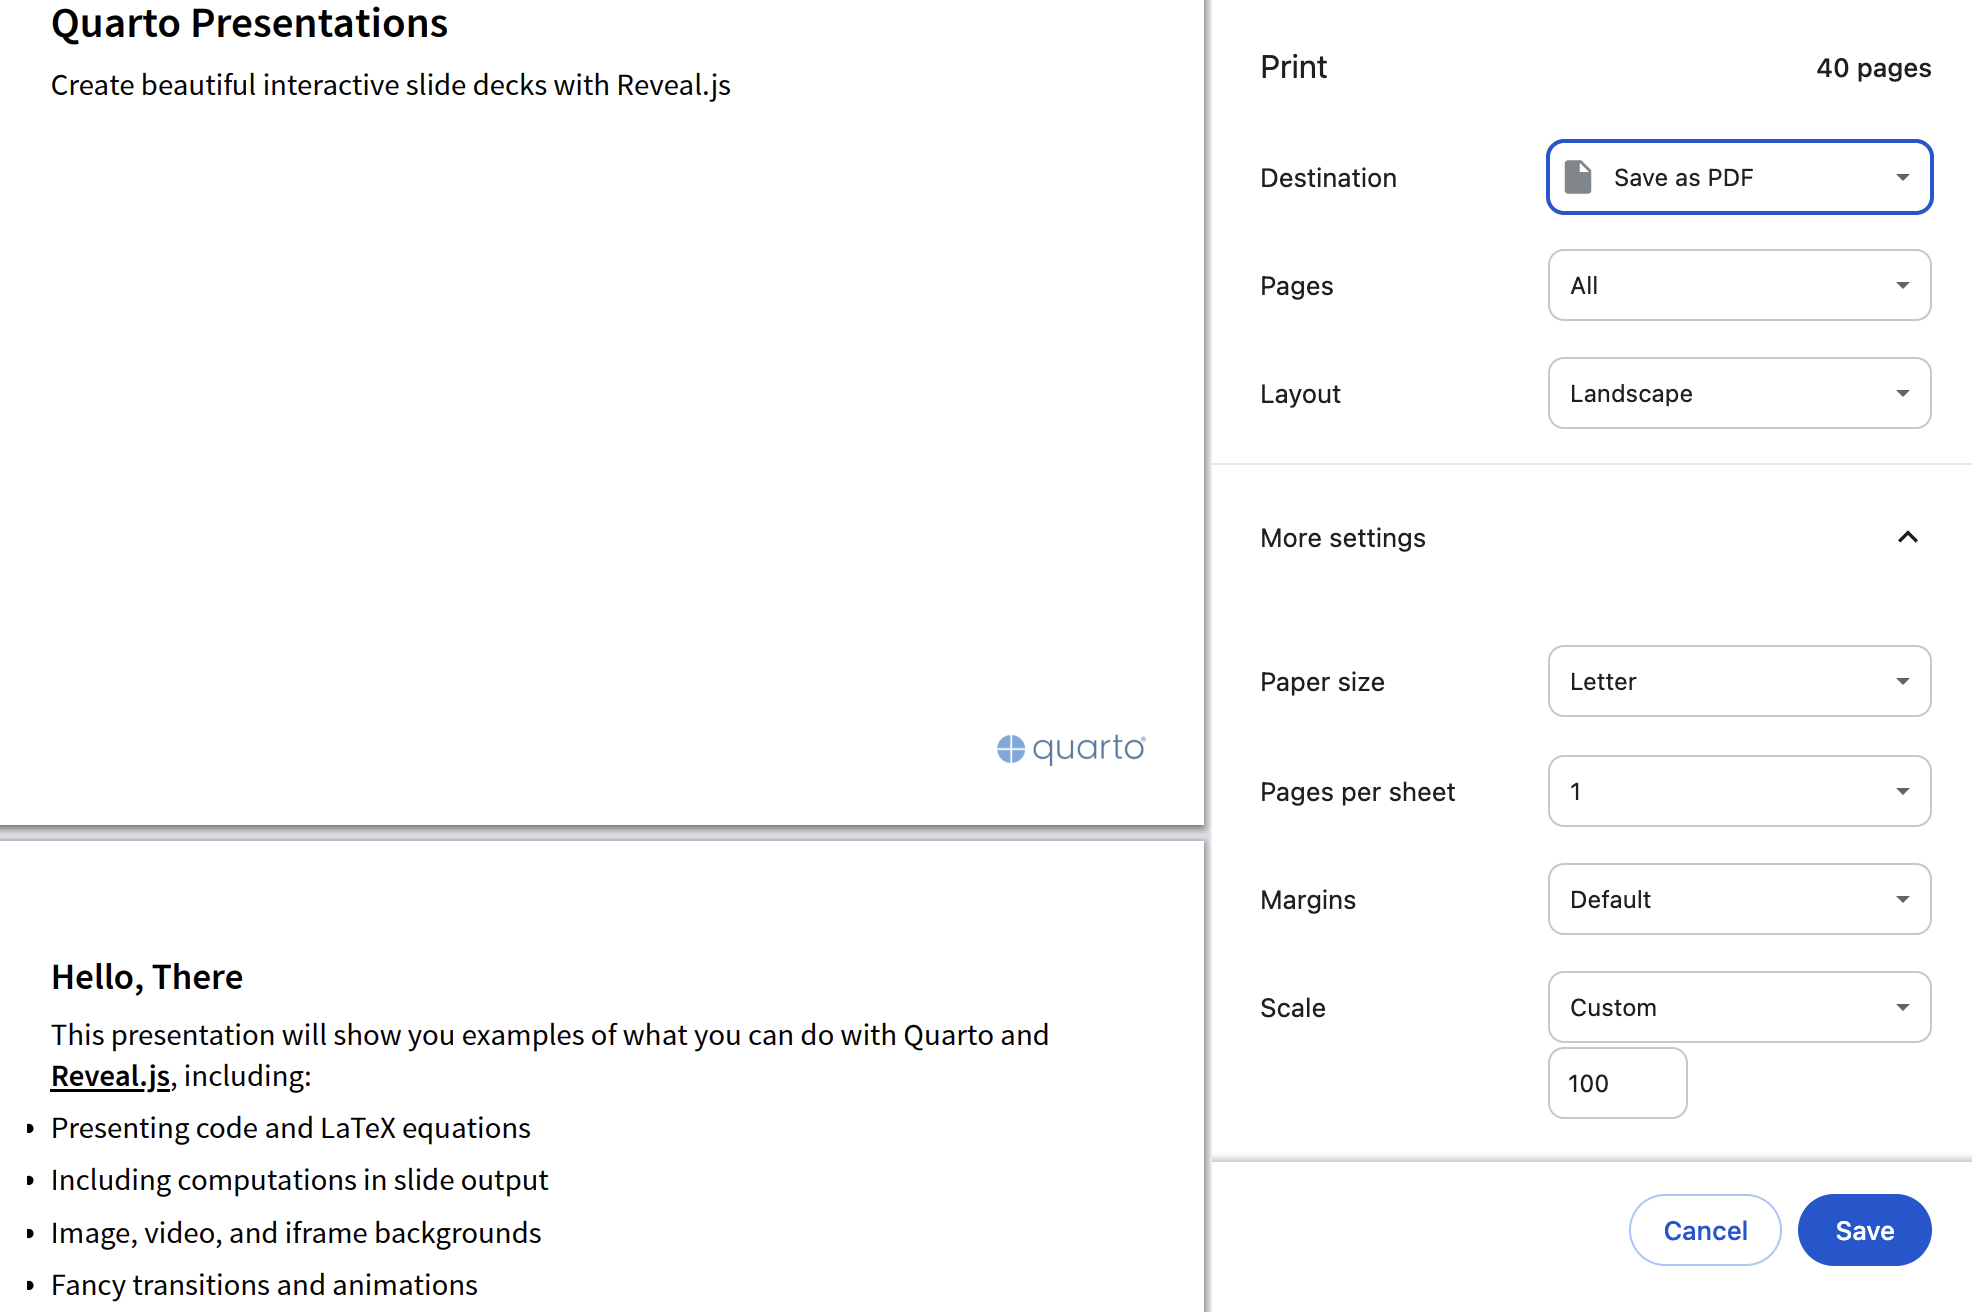
\includegraphics[keepaspectratio]{presentation/images/clipboard-1451207711.png}}

A PDF presentation should have only one slide per page, but putting
multiple slides on one page may be convenient if we want to read the
slides instead of presenting them.

\pandocbounded{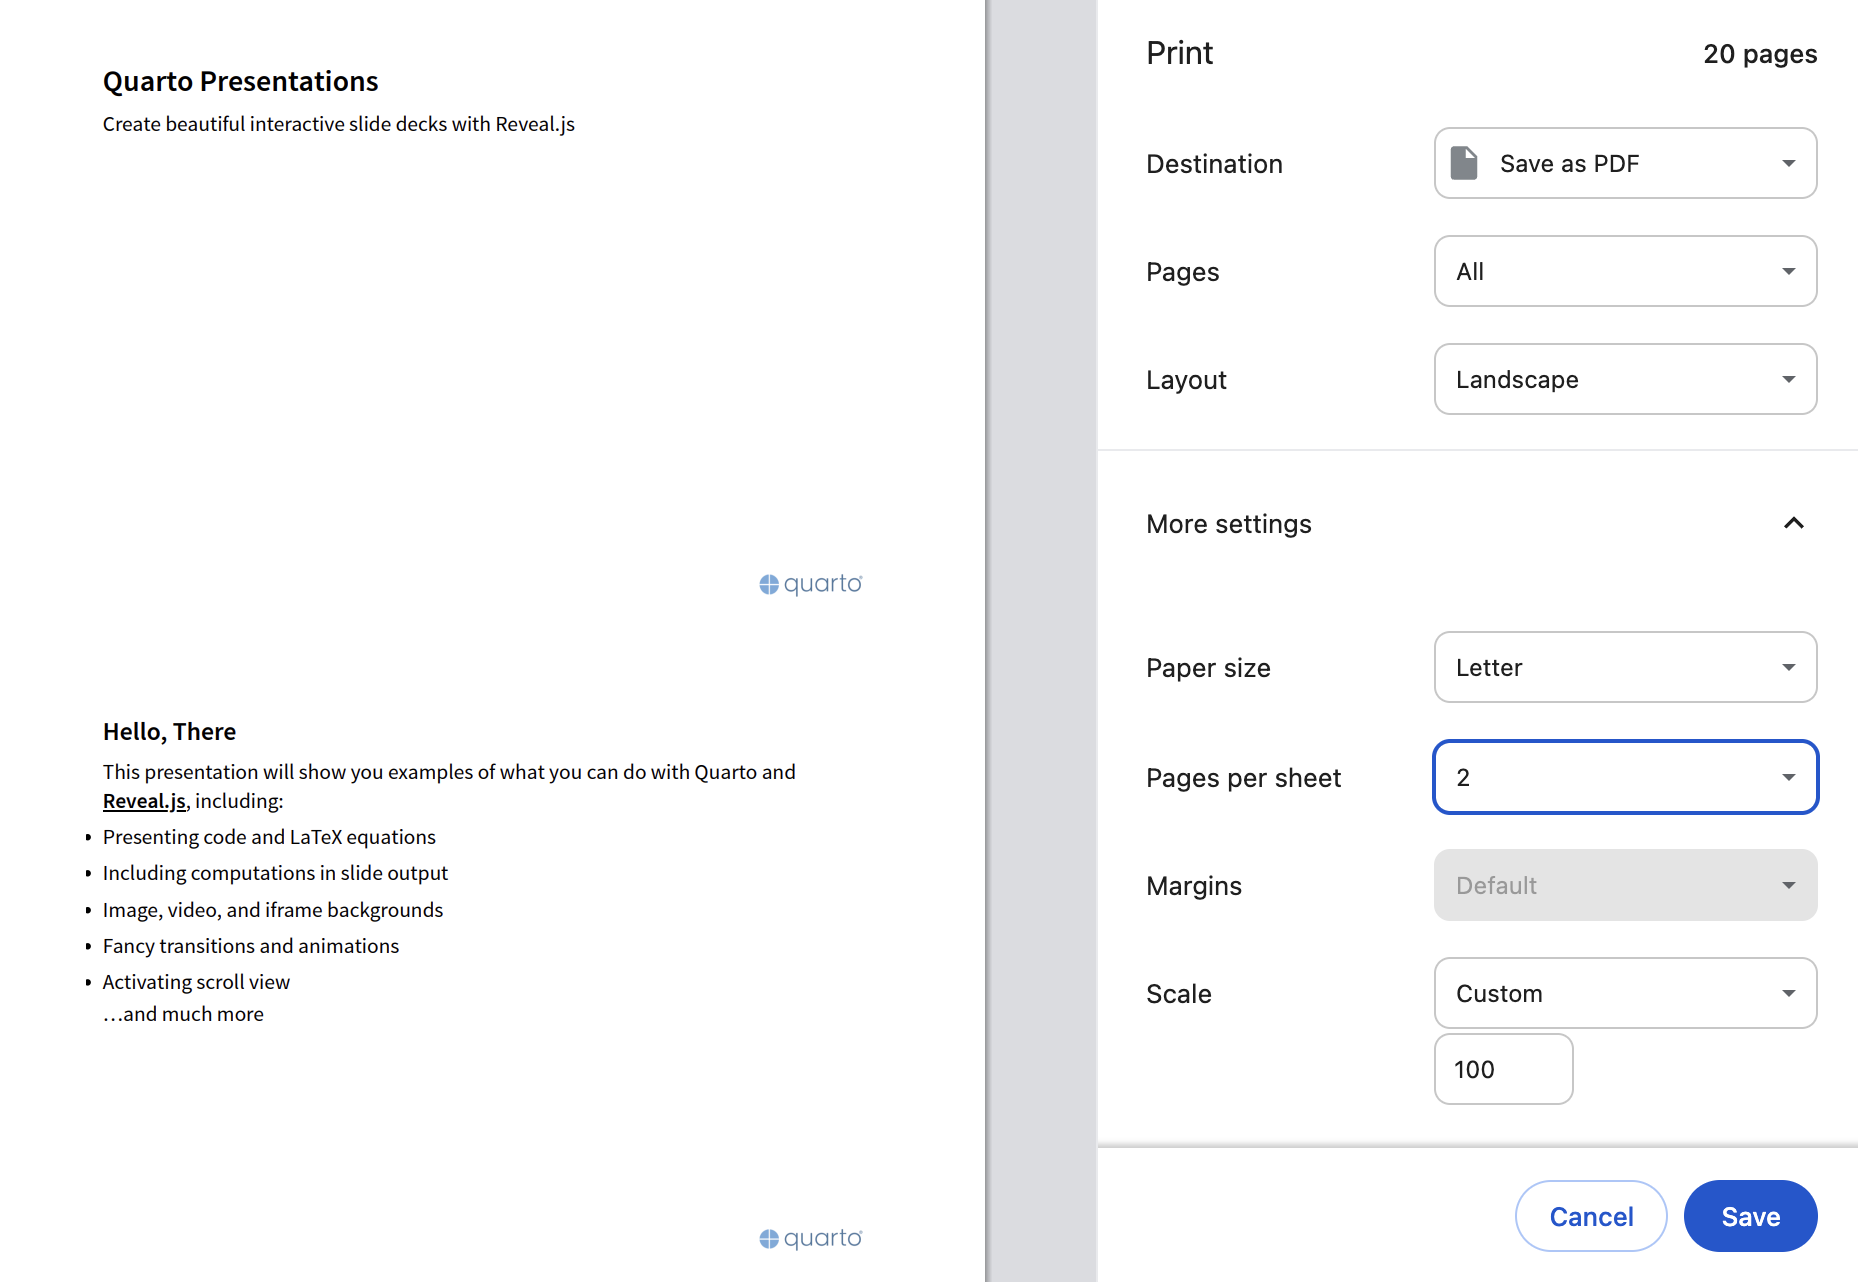
\includegraphics[keepaspectratio]{presentation/images/clipboard-4067504015.png}}

For best results, I suggest following the PDF export instructions in the
\href{https://revealjs.com}{RevealJS} documentation:
\url{https://revealjs.com/pdf-export/}.

PDF files are ubiquitous and it is good to know that you can generate
one with nothing more than a web browser whenever necessary, but HTML
files can do many things that PDF files simply cannot.

The HTML presentation below demonstrates all of the features described
in its slides, many of which are not active in the PDF presentation
beneath it.

Instead of embedding your presentation in a webpage as shown above, you
can view it in its own browser tab in \href{demo/}{HTML} or
\href{demo/demo.pdf}{PDF} format.

To edit a presentation, you can modify the plain text of the associated
qmd file in a \href{https://en.wikipedia.org/wiki/Text_editor}{text
editor} or work with a
\href{https://en.wikipedia.org/wiki/WYSIWYG}{WYSIWYG} version via the
\href{https://docs.posit.co/ide/user/ide/guide/documents/visual-editor.html}{Visual
Mode} in RStudio, VSCode, Codespaces, or Positron.

When you want to update the presentation on your website, all you have
to do is add, commit, and push your changes. It may take some time for
your site to update after you push changes. You can see the status and
logs of all of your website builds in the Actions tab of your repo on
\textless github.com\textgreater.




\end{document}
